%\RequirePackage[l2tabu,orthodox]{nag} % Раскомментировав, можно в логе получать рекомендации относительно правильного использования пакетов и предупреждения об устаревших и нерекомендуемых пакетах
% Формат А4, 14pt (ГОСТ Р 7.0.11-2011, 5.3.6)
\documentclass[a4paper,14pt]{extreport}

%%% Проверка используемого TeX-движка %%%
\usepackage{iftex}
\newif\ifxetexorluatex   % определяем новый условный оператор (http://tex.stackexchange.com/a/47579/79756)
\ifXeTeX
    \xetexorluatextrue
\else
    \ifLuaTeX
        \xetexorluatextrue
    \else
        \xetexorluatexfalse
    \fi
\fi

%%% Поля и разметка страницы %%%
\usepackage{pdflscape}                              % Для включения альбомных страниц
\usepackage{geometry}                               % Для последующего задания полей

%%% Математические пакеты %%%
\usepackage{amsthm,amsfonts,amsmath,amssymb,amscd}  % Математические дополнения от AMS
\usepackage{mathtools}                              % Добавляет окружение multlined

%%%% Установки для размера шрифта 14 pt %%%%
%% Формирование переменных и констант для сравнения (один раз для всех подключаемых файлов)%%
%% должно располагаться до вызова пакета fontspec или polyglossia, потому что они сбивают его работу
\newlength{\curtextsize}
\newlength{\bigtextsize}
\setlength{\bigtextsize}{13.9pt}

\makeatletter
%\show\f@size                                       % неплохо для отслеживания, но вызывает стопорение процесса, если документ компилируется без команды  -interaction=nonstopmode 
\setlength{\curtextsize}{\f@size pt}
\makeatother

%%% Кодировки и шрифты %%%
\ifxetexorluatex
    \usepackage{polyglossia}                        % Поддержка многоязычности (fontspec подгружается автоматически)
\else
    \RequirePDFTeX                                  % tests for PDFTEX use and throws an error if a different engine is being used
   %%% Решение проблемы копирования текста в буфер кракозябрами
%    \input glyphtounicode.tex
%    \input glyphtounicode-cmr.tex %from pdfx package
%    \pdfgentounicode=1
    \usepackage{cmap}                               % Улучшенный поиск русских слов в полученном pdf-файле
    \defaulthyphenchar=127                          % Если стоит до fontenc, то переносы не впишутся в выделяемый текст при копировании его в буфер обмена
    \usepackage[T2A]{fontenc}                       % Поддержка русских букв
    \usepackage[utf8]{inputenc}                     % Кодировка utf8
    \usepackage[english, russian]{babel}            % Языки: русский, английский
    \IfFileExists{pscyr.sty}{\usepackage{pscyr}}{}  % Красивые русские шрифты
\fi

%%% Оформление абзацев %%%
\usepackage{indentfirst}                            % Красная строка

%%% Цвета %%%
\usepackage[dvipsnames,usenames]{color}
\usepackage{colortbl}
%\usepackage[dvipsnames, table, hyperref, cmyk]{xcolor} % Вероятно, более новый вариант, вместо предыдущих двух строк. Конвертация всех цветов в cmyk заложена как удовлетворение возможного требования типографий. Возможно конвертирование и в rgb.

%%% Таблицы %%%
\usepackage{longtable}                              % Длинные таблицы
\usepackage{multirow,makecell,array}                % Улучшенное форматирование таблиц
\usepackage{booktabs}                               % Возможность оформления таблиц в классическом книжном стиле (при правильном использовании не противоречит ГОСТ)

%%% Общее форматирование
\usepackage{soulutf8}                               % Поддержка переносоустойчивых подчёркиваний и зачёркиваний
\usepackage{icomma}                                 % Запятая в десятичных дробях


%%% Гиперссылки %%%
\usepackage{hyperref}

%%% Изображения %%%
\usepackage{graphicx}                               % Подключаем пакет работы с графикой

%%% Списки %%%
\usepackage{enumitem}

%%% Подписи %%%
\usepackage{caption}                                % Для управления подписями (рисунков и таблиц) % Может управлять номерами рисунков и таблиц с caption %Иногда может управлять заголовками в списках рисунков и таблиц
\usepackage{subcaption}                             % Работа с подрисунками и подобным

%%% Интервалы %%%
\usepackage[onehalfspacing]{setspace}               % Опция запуска пакета правит не только интервалы в обычном тексте, но и формульные

%%% Счётчики %%%
\usepackage[figure,table]{totalcount}               % Счётчик рисунков и таблиц
\usepackage{totcount}                               % Пакет создания счётчиков на основе последнего номера подсчитываемого элемента (может требовать дважды компилировать документ)
\usepackage{totpages}                               % Счётчик страниц, совместимый с hyperref (ссылается на номер последней страницы). Желательно ставить последним пакетом в преамбуле

%%% Продвинутое управление групповыми ссылками (пока только формулами) %%%
\ifxetexorluatex
    \usepackage{cleveref}                           % cleveref корректно считывает язык из настроек polyglossia
\else
    \usepackage[russian]{cleveref}                  % cleveref имеет сложности со считыванием языка из babel. Такое решение русификации вывода выбрано вместо определения в documentclass из опасности что-то лишнее передать во все остальные пакеты, включая библиографию.
\fi
\creflabelformat{equation}{#2#1#3}                  % Формат по умолчанию ставил круглые скобки вокруг каждого номера ссылки, теперь просто номера ссылок без какого-либо дополнительного оформления

  % Пакеты общие для диссертации и автореферата
%%% Колонтитулы %%%
\usepackage{fancyhdr}

%%% Прикладные пакеты %%% 
\usepackage{calc}               % Пакет для расчётов параметров, например длины
%\usepackage{etoolbox}          % ради функции patchcmd для управления списком литературы

\usepackage {interfaces-base}   % Набор базовых интерфейсов к некоторым пакетам, конкретные реализации загружаются в стиле

%%% Заголовки %%%
\usepackage{titlesec}           % Пакет настройки шрифтов заголовков в тексте

%%% Оглавление %%%
\usepackage{tocloft}

%%% Счётчики %%%
\usepackage{chngcntr}           % оперативная перенастройка счётчиков         % Пакеты для диссертации
\usepackage{tabularx,tabulary}  %таблицы с автоматически подбирающейся шириной столбцов

% Листинги с исходным кодом программ
\usepackage{fancyvrb}
\usepackage{listings}

% Плавающие окружения. во многом лучше пакета float
\usepackage{floatrow}

% Русская традиция начертания греческих букв
%\usepackage{upgreek} % прямые греческие ради русской традиции        % Пакеты для специфических пользовательских задач
\newcommand{\angstrom}{\mbox{\normalfont\AA}}
%\usepackage[pdftex]{lscape}
\usepackage{lineno}
%\linenumbers

%%%%%%%%%%%%%%%%%%%%%%%%%%%%%%%%%%%%%%%%%%%%%%%%%%%%%%
%%%% Файл упрощённых настроек шаблона диссертации %%%%
%%%%%%%%%%%%%%%%%%%%%%%%%%%%%%%%%%%%%%%%%%%%%%%%%%%%%%

%%%        Подключение пакетов                 %%%
\usepackage{ifthen}                 % добавляет ifthenelse
%%% Инициализирование переменных, не трогать!  %%%
\newcounter{intvl}
\newcounter{otstup}
\newcounter{contnumeq}
\newcounter{contnumfig}
\newcounter{contnumtab}
\newcounter{pgnum}
\newcounter{bibliosel}
\newcounter{chapstyle}
\newcounter{headingdelim}
\newcounter{headingalign}
\newcounter{headingsize}
\newcounter{tabcap}
\newcounter{tablaba}
\newcounter{tabtita}
%%%%%%%%%%%%%%%%%%%%%%%%%%%%%%%%%%%%%%%%%%%%%%%%%%

%%% Область упрощённого управления оформлением %%%

%% Интервал между заголовками и между заголовком и текстом
% Заголовки отделяют от текста сверху и снизу тремя интервалами (ГОСТ Р 7.0.11-2011, 5.3.5)
\setcounter{intvl}{3}               % Коэффициент кратности к размеру шрифта

%% Отступы у заголовков в тексте
\setcounter{otstup}{0}              % 0 --- без отступа; 1 --- абзацный отступ

%% Нумерация формул, таблиц и рисунков
\setcounter{contnumeq}{0}           % Нумерация формул: 0 --- пораздельно (во введении подряд, без номера раздела); 1 --- сквозная нумерация по всей диссертации
\setcounter{contnumfig}{0}          % Нумерация рисунков: 0 --- пораздельно (во введении подряд, без номера раздела); 1 --- сквозная нумерация по всей диссертации
\setcounter{contnumtab}{1}          % Нумерация таблиц: 0 --- пораздельно (во введении подряд, без номера раздела); 1 --- сквозная нумерация по всей диссертации

%% Оглавление
\setcounter{pgnum}{1}               % 0 --- номера страниц никак не обозначены; 1 --- Стр. над номерами страниц (дважды компилировать после изменения)

%% Библиография
\setcounter{bibliosel}{1}           % 0 --- встроенная реализация с загрузкой файла через движок bibtex8; 1 --- реализация пакетом biblatex через движок biber

%% Текст и форматирование заголовков
\setcounter{chapstyle}{1}           % 0 --- разделы только под номером; 1 --- разделы с названием "Глава" перед номером
\setcounter{headingdelim}{1}        % 0 --- номер отделен пропуском в 1em или \quad; 1 --- номера разделов и приложений отделены точкой с пробелом, подразделы пропуском без точки; 2 --- номера разделов, подразделов и приложений отделены точкой с пробелом.

%% Выравнивание заголовков в тексте
\setcounter{headingalign}{0}        % 0 --- по центру; 1 --- по левому краю

%% Размеры заголовков в тексте
\setcounter{headingsize}{0}         % 0 --- по ГОСТ, все всегда 14 пт; 1 --- пропорционально изменяющийся размер в зависимости от базового шрифта

%% Подпись таблиц
\setcounter{tabcap}{0}              % 0 --- по ГОСТ, номер таблицы и название разделены тире, выровнены по левому краю, при необходимости на нескольких строках; 1 --- подпись таблицы не по ГОСТ, на двух и более строках, дальнейшие настройки: 
%Выравнивание первой строки, с подписью и номером
\setcounter{tablaba}{2}             % 0 --- по левому краю; 1 --- по центру; 2 --- по правому краю
%Выравнивание строк с самим названием таблицы
\setcounter{tabtita}{1}             % 0 --- по левому краю; 1 --- по центру; 2 --- по правому краю

%%% Цвета гиперссылок %%%
% Latex color definitions: http://latexcolor.com/
\definecolor{linkcolor}{rgb}{0.9,0,0}
\definecolor{citecolor}{rgb}{0,0.6,0}
\definecolor{urlcolor}{rgb}{0,0,1}
%\definecolor{linkcolor}{rgb}{0,0,0} %black
%\definecolor{citecolor}{rgb}{0,0,0} %black
%\definecolor{urlcolor}{rgb}{0,0,0} %black               % Упрощённые настройки шаблона

%%% Переопределение именований, чтобы можно было и в преамбуле использовать %%%
\renewcommand{\chaptername}{Глава}
\renewcommand{\appendixname}{Приложение} % (ГОСТ Р 7.0.11-2011, 5.7)
       % Переопределение именований, чтобы можно было и в преамбуле использовать
% Новые переменные, которые могут использоваться во всём проекте
\newcommand{\authorbibtitle}{Публикации автора}
\newcommand{\fullbibtitle}{Список литературы} % (ГОСТ Р 7.0.11-2011, 4)
  % Новые переменные, которые могут использоваться во всём проекте

%%% Основные сведения %%%
\newcommand{\thesisAuthor}             % Диссертация, ФИО автора
{%
    \texorpdfstring{% \texorpdfstring takes two arguments and uses the first for (La)TeX and the second for pdf
        {Ярославцев Алексей Алексеевич}% так будет отображаться на титульном листе или в тексте, где будет использоваться переменная
    }{%
        Ярославцев, Алексей Алексеевич% эта запись для свойств pdf-файла. В таком виде, если pdf будет обработан программами для сбора библиографических сведений, будет правильно представлена фамилия.
    }%
}
\newcommand{\thesisUdk}                % Диссертация, УДК
{\todo{xxx.xxx}}
\newcommand{\thesisTitle}              % Диссертация, название
{\texorpdfstring{{\textbf{ВЛИЯНИЕ ЛОКАЛЬНОГО ОКРУЖЕНИЯ МЕДИ НА МАГНИТНЫЕ И ТРАНСПОРТНЫЕ СВОЙСТВА СОЕДИНЕНИЙ ГРУППЫ ТЕТРАЭДРИТА-ТЕННАНТИТА}}}{Название диссертационной работы}}

%ВЛИЯНИЕ ИЗОВАЛЕТНОГО ЗАМЕЩЕНИЯ В СОЕДИНЕНИЯХ Cu\textsubscript{12}V\textsubscript{4}VI\textsubscript{13} (V~=~As,~Sb И VI~=~S,~Se) НА МАГНИТНЫЕ И ТРАНСПОРТНЫЕ СВОЙСТВА

\newcommand{\thesisSpecialtyNumber}    % Диссертация, специальность, номер
{\texorpdfstring{{01.03.08}}{XX.XX.XX}}
\newcommand{\thesisSpecialtyTitle}     % Диссертация, специальность, название
{\texorpdfstring{{Физика конденсированного состояния}}{Название специальности}}
\newcommand{\thesisDegree}             % Диссертация, научная степень
{{кандидата физико-математических наук}}
\newcommand{\thesisCity}               % Диссертация, город защиты
{{Москва}}
\newcommand{\thesisYear}               % Диссертация, год защиты
{{2021}}
\newcommand{\thesisOrganization}       % Диссертация, организация
{{Федеральное государственное бюджетное научное учреждение «Технологический институт сверхтвердых и новых углеродных материалов», (ФГБНУ ТИСНУМ)}}

\newcommand{\thesisInOrganization}       % Диссертация, организация в предложном падеже: Работа выполнена в ...
{{Федеральном государственном бюджетном научном учреждении «Технологический институт сверхтвердых и новых углеродных материалов» (ФГБНУ ТИСНУМ).}}

\newcommand{\supervisorFio}            % Научный руководитель, ФИО
{Буга Сергей Геннадьевич}
\newcommand{\supervisorRegalia}        % Научный руководитель, регалии
{доктор физико-математических наук, доцент}

\newcommand{\opponentOneFio}           % Оппонент 1, ФИО
{\todo{Фамилия Имя Отчество}}
\newcommand{\opponentOneRegalia}       % Оппонент 1, регалии
{\todo{доктор физико-математических наук, профессор}}
\newcommand{\opponentOneJobPlace}      % Оппонент 1, место работы
{\todo{Не очень длинное название для места работы}}
\newcommand{\opponentOneJobPost}       % Оппонент 1, должность
{\todo{старший научный сотрудник}}

\newcommand{\opponentTwoFio}           % Оппонент 2, ФИО
{\todo{Фамилия Имя Отчество}}
\newcommand{\opponentTwoRegalia}       % Оппонент 2, регалии
{\todo{кандидат физико-математических наук}}
\newcommand{\opponentTwoJobPlace}      % Оппонент 2, место работы
{\todo{Основное место работы c длинным длинным длинным длинным названием}}
\newcommand{\opponentTwoJobPost}       % Оппонент 2, должность
{\todo{старший научный сотрудник}}

\newcommand{\leadingOrganizationTitle} % Ведущая организация, дополнительные строки
{\todo{Федеральное государственное бюджетное образовательное учреждение высшего профессионального образования с~длинным длинным длинным длинным названием}}

\newcommand{\defenseDate}              % Защита, дата
{\todo{DD mmmmmmmm YYYY~г.~в~XX часов}}
\newcommand{\defenseCouncilNumber}     % Защита, номер диссертационного совета
{\todo{NN}}
\newcommand{\defenseCouncilTitle}      % Защита, учреждение диссертационного совета
{\todo{Название учреждения}}
\newcommand{\defenseCouncilAddress}    % Защита, адрес учреждение диссертационного совета
{\todo{Адрес}}

\newcommand{\defenseSecretaryFio}      % Секретарь диссертационного совета, ФИО
{\todo{Фамилия Имя Отчество}}
\newcommand{\defenseSecretaryRegalia}  % Секретарь диссертационного совета, регалии
{\todo{д-р~физ.-мат. наук}}            % Для сокращений есть ГОСТы, например: ГОСТ Р 7.0.12-2011 + http://base.garant.ru/179724/#block_30000

\newcommand{\synopsisLibrary}          % Автореферат, название библиотеки
{\todo{Название библиотеки}}
\newcommand{\synopsisDate}             % Автореферат, дата рассылки
{\todo{DD mmmmmmmm YYYY года}}

\newcommand{\keywords}%                 % Ключевые слова для метаданных PDF диссертации и автореферата
{}      % Основные сведения
%%% Макет страницы %%%
% Выставляем значения полей (ГОСТ 7.0.11-2011, 5.3.7)
\geometry{a4paper,top=2cm,bottom=2cm,left=2.5cm,right=1cm}

%%% Кодировки и шрифты %%%
\ifxetexorluatex
    \setmainlanguage[babelshorthands=true]{russian}  % Язык по-умолчанию русский с поддержкой приятных команд пакета babel
    \setotherlanguage{english}                       % Дополнительный язык = английский (в американской вариации по-умолчанию)
    \ifXeTeX
        \defaultfontfeatures{Ligatures=TeX,Mapping=tex-text}
    \else
        \defaultfontfeatures{Ligatures=TeX}
    \fi
    \setmainfont{Times New Roman}
    \newfontfamily\cyrillicfont{Times New Roman}
    \setsansfont{Arial}
    \newfontfamily\cyrillicfontsf{Arial}
    \setmonofont{Courier New}
    \newfontfamily\cyrillicfonttt{Courier New}
\else
    \IfFileExists{pscyr.sty}{\renewcommand{\rmdefault}{ftm}}{}
\fi

%%% Интервалы %%%
%linespread-реализация ближе к реализации полуторного интервала в ворде.
%setspace реализация заточена под шрифты 10, 11, 12pt, под остальные кегли хуже, но всё же ближе к типографской классике. 
%\linespread{1.3}                    % Полуторный интервал (ГОСТ Р 7.0.11-2011, 5.3.6)

%%% Выравнивание и переносы %%%
\sloppy                             % Избавляемся от переполнений
\clubpenalty=10000                  % Запрещаем разрыв страницы после первой строки абзаца
\widowpenalty=10000                 % Запрещаем разрыв страницы после последней строки абзаца

%%% Подписи %%%
\captionsetup{%
singlelinecheck=off,                % Многострочные подписи, например у таблиц
skip=2pt,                           % Вертикальная отбивка между подписью и содержимым рисунка или таблицы определяется ключом
justification=centering,            % Центрирование подписей, заданных командой \caption
}

%%% Рисунки %%%
\DeclareCaptionLabelSeparator*{emdash}{~--- }             % (ГОСТ 2.105, 4.3.1)
\captionsetup[figure]{labelsep=emdash,font=onehalfspacing,position=bottom}

%%% Таблицы %%%
\ifthenelse{\equal{\thetabcap}{0}}{%
    \newcommand{\tabcapalign}{\raggedright}  % по левому краю страницы или аналога parbox
}

\ifthenelse{\equal{\thetablaba}{0} \AND \equal{\thetabcap}{1}}{%
    \newcommand{\tabcapalign}{\raggedright}  % по левому краю страницы или аналога parbox
}

\ifthenelse{\equal{\thetablaba}{1} \AND \equal{\thetabcap}{1}}{%
    \newcommand{\tabcapalign}{\centering}    % по центру страницы или аналога parbox
}

\ifthenelse{\equal{\thetablaba}{2} \AND \equal{\thetabcap}{1}}{%
    \newcommand{\tabcapalign}{\raggedleft}   % по правому краю страницы или аналога parbox
}

\ifthenelse{\equal{\thetabtita}{0} \AND \equal{\thetabcap}{1}}{%
    \newcommand{\tabtitalign}{\raggedright}  % по левому краю страницы или аналога parbox
}

\ifthenelse{\equal{\thetabtita}{1} \AND \equal{\thetabcap}{1}}{%
    \newcommand{\tabtitalign}{\centering}    % по центру страницы или аналога parbox
}

\ifthenelse{\equal{\thetabtita}{2} \AND \equal{\thetabcap}{1}}{%
    \newcommand{\tabtitalign}{\raggedleft}   % по правому краю страницы или аналога parbox
}

\DeclareCaptionFormat{tablenocaption}{\tabcapalign #1\strut}        % Наименование таблицы отсутствует
\ifthenelse{\equal{\thetabcap}{0}}{%
    \DeclareCaptionFormat{tablecaption}{\tabcapalign #1#2#3}
    \captionsetup[table]{labelsep=emdash}                       % тире как разделитель идентификатора с номером от наименования
}{%
    \DeclareCaptionFormat{tablecaption}{\tabcapalign #1#2\par%  % Идентификатор таблицы на отдельной строке
        \tabtitalign{#3}}                                       % Наименование таблицы строкой ниже
    \captionsetup[table]{labelsep=space}                        % пробельный разделитель идентификатора с номером от наименования
}
\captionsetup[table]{format=tablecaption,singlelinecheck=off,font=onehalfspacing,position=top,skip=0pt}  % многострочные наименования и прочее
\DeclareCaptionLabelFormat{continued}{Продолжение таблицы~#2}

%%% Подписи подрисунков %%%
\renewcommand{\thesubfigure}{\asbuk{subfigure}}           % Буквенные номера подрисунков
\captionsetup[subfigure]{font={normalsize},               % Шрифт подписи названий подрисунков (не отличается от основного)
    labelformat=brace,                                    % Формат обозначения подрисунка
    justification=centering,                              % Выключка подписей (форматирование), один из вариантов            
}
%\DeclareCaptionFont{font12pt}{\fontsize{12pt}{13pt}\selectfont} % объявляем шрифт 12pt для использования в подписях, тут же надо интерлиньяж объявлять, если не наследуется
%\captionsetup[subfigure]{font={font12pt}}                 % Шрифт подписи названий подрисунков (всегда 12pt)

%%% Настройки гиперссылок %%%
\ifLuaTeX
    \hypersetup{
        unicode,                % Unicode encoded PDF strings
    }
\fi

\hypersetup{
    linktocpage=true,           % ссылки с номера страницы в оглавлении, списке таблиц и списке рисунков
%    linktoc=all,                % both the section and page part are links
%    pdfpagelabels=false,        % set PDF page labels (true|false)
    plainpages=false,           % Forces page anchors to be named by the Arabic form  of the page number, rather than the formatted form
    colorlinks,                 % ссылки отображаются раскрашенным текстом, а не раскрашенным прямоугольником, вокруг текста
    linkcolor={linkcolor},      % цвет ссылок типа ref, eqref и подобных
    citecolor={citecolor},      % цвет ссылок-цитат
    urlcolor={urlcolor},        % цвет гиперссылок
%    hidelinks,                  % Hide links (removing color and border)
    pdftitle={\thesisTitle},    % Заголовок
    pdfauthor={\thesisAuthor},  % Автор
    pdfsubject={\thesisSpecialtyNumber\ \thesisSpecialtyTitle},      % Тема
%    pdfcreator={Создатель},     % Создатель, Приложение
%    pdfproducer={Производитель},% Производитель, Производитель PDF
    pdfkeywords={\keywords},    % Ключевые слова
    pdflang={ru},
}

%%% Шаблон %%%
\DeclareRobustCommand{\todo}{\textcolor{red}}       % решаем проблему превращения названия цвета в результате \MakeUppercase, http://tex.stackexchange.com/a/187930/79756 , \DeclareRobustCommand protects \todo from expanding inside \MakeUppercase
\setlength{\parindent}{2.5em}                       % Абзацный отступ. Должен быть одинаковым по всему тексту и равен пяти знакам (ГОСТ Р 7.0.11-2011, 5.3.7).

%%% Списки %%%
% Используем дефис для ненумерованных списков (ГОСТ 2.105-95, 4.1.7)
\renewcommand{\labelitemi}{\normalfont\bfseries{--}} 
\setlist{nosep,%                                    % Единый стиль для всех списков (пакет enumitem), без дополнительных интервалов.
    labelindent=\parindent,leftmargin=*%            % Каждый пункт, подпункт и перечисление записывают с абзацного отступа (ГОСТ 2.105-95, 4.1.8)
}
    % Стили общие для диссертации и автореферата
%%% Изображения %%%
\graphicspath{{images/}{Dissertation/images/}}         % Пути к изображениям

\LoadInterface {titlesec}                   % Подгружаем интерфейсы для дополнительных опций управления некоторыми пакетами

%%% Блок управления параметрами для выравнивания заголовков в тексте %%%
\newlength{\otstuplen}
\setlength{\otstuplen}{\theotstup\parindent}
\ifthenelse{\equal{\theheadingalign}{0}}{% выравнивание заголовков в тексте
    \newcommand{\hdngalign}{\filcenter}                % по центру
    \newcommand{\hdngaligni}{\hfill\hspace{\otstuplen}}% по центру
}{%
    \newcommand{\hdngalign}{\filright}                 % по левому краю
    \newcommand{\hdngaligni}{\hspace{\otstuplen}}      % по левому краю
} % В обоих случаях вроде бы без переноса, как и надо (ГОСТ Р 7.0.11-2011, 5.3.5)

%%% Оглавление %%%
\renewcommand{\cftchapdotsep}{\cftdotsep}                % отбивка точками до номера страницы начала главы/раздела
\renewcommand{\cfttoctitlefont}{\hdngaligni\fontsize{14pt}{16pt}\selectfont\bfseries}% вместе со следующей строкой
\renewcommand{\cftaftertoctitle}{\hfill}                 % устанавливает заголовок по центру
\setlength{\cftbeforetoctitleskip}{-1.4\curtextsize}     % Поскольку этот заголовок всегда является первым на странице, то перед ним отделять пустым тройным интервалом не следует. Независимо от основного шрифта, в этом случае зануление (почти) происходит при -1.4\curtextsize.
\setlength{\cftaftertoctitleskip}{\theintvl\curtextsize} % Если считаем Оглавление заголовком, то выставляем после него тройной интервал через наше определённое значение

%% Переносить слова в заголовке не допускается (ГОСТ Р 7.0.11-2011, 5.3.5). Заголовки в оглавлении должны точно повторять заголовки в тексте (ГОСТ Р 7.0.11-2011, 5.2.3). Прямого указания на запрет переносов в оглавлении нет, но по той же логике невнесения искажений в смысл, лучше в оглавлении не переносить:
\cftsetrmarg{2.55em plus1fil}                       %To have the (sectional) titles in the ToC, etc., typeset ragged right with no hyphenation
\renewcommand{\cftchappagefont}{\normalfont}        % нежирные номера страниц у глав в оглавлении
\renewcommand{\cftchapleader}{\cftdotfill{\cftchapdotsep}}% нежирные точки до номеров страниц у глав в оглавлении
%\renewcommand{\cftchapfont}{}                       % нежирные названия глав в оглавлении

\ifthenelse{\theheadingdelim > 0}{%
    \renewcommand\cftchapaftersnum{.\ }   % добавляет точку с пробелом после номера раздела в оглавлении
}{%
\renewcommand\cftchapaftersnum{\quad}     % добавляет \quad после номера раздела в оглавлении
}
\ifthenelse{\theheadingdelim > 1}{%
    \renewcommand\cftsecaftersnum{.\ }    % добавляет точку с пробелом после номера подраздела в оглавлении
    \renewcommand\cftsubsecaftersnum{.\ } % добавляет точку с пробелом после номера подподраздела в оглавлении
}{%
\renewcommand\cftsecaftersnum{\quad}      % добавляет \quad после номера подраздела в оглавлении
\renewcommand\cftsubsecaftersnum{\quad}   % добавляет \quad после номера подподраздела в оглавлении
}

\ifthenelse{\equal{\thepgnum}{1}}{%
    \addtocontents{toc}{~\hfill{Стр.}\par}% добавить Стр. над номерами страниц
}

%%% Оформление названий глав %%%
%% настройки заголовка списка рисунков
\renewcommand{\cftloftitlefont}{\hdngaligni\fontsize{14pt}{16pt}\selectfont\bfseries}% вместе со следующей строкой
\renewcommand{\cftafterloftitle}{\hfill}                                             % устанавливает заголовок по центру
\setlength{\cftbeforeloftitleskip}{-1.5\curtextsize}     % Поскольку этот заголовок всегда является первым на странице, то перед ним отделять пустым тройным интервалом не следует. Независимо от основного шрифта, в этом случае зануление (почти) происходит при -1.5\curtextsize.
\setlength{\cftafterloftitleskip}{\theintvl\curtextsize} % выставляем после него тройной интервал через наше определённое значение

%% настройки заголовка списка таблиц
\renewcommand{\cftlottitlefont}{\hdngaligni\fontsize{14pt}{16pt}\selectfont\bfseries}% вместе со следующей строкой
\renewcommand{\cftafterlottitle}{\hfill}                                             % устанавливает заголовок по центру
\setlength{\cftbeforelottitleskip}{-1.5\curtextsize}     % Поскольку этот заголовок всегда является первым на странице, то перед ним отделять пустым тройным интервалом не следует. Независимо от основного шрифта, в этом случае зануление (почти) происходит при -1.5\curtextsize.
\setlength{\cftafterlottitleskip}{\theintvl\curtextsize} % выставляем после него тройной интервал через наше определённое значение

\ifnum\curtextsize>\bigtextsize     % Проверяем условие использования базового шрифта 14 pt
\setlength{\headheight}{17pt}       % Исправляем высоту заголовка
\else
\setlength{\headheight}{15pt}       % Исправляем высоту заголовка
\fi

%%% Колонтитулы %%%
% Порядковый номер страницы печатают на середине верхнего поля страницы (ГОСТ Р 7.0.11-2011, 5.3.8)
\makeatletter
\let\ps@plain\ps@fancy              % Подчиняем первые страницы каждой главы общим правилам
\makeatother
\pagestyle{fancy}                   % Меняем стиль оформления страниц
\fancyhf{}                          % Очищаем текущие значения
\fancyhead[C]{\thepage}             % Печатаем номер страницы на середине верхнего поля
\renewcommand{\headrulewidth}{0pt}  % Убираем разделительную линию

%%% Оформление заголовков глав, разделов, подразделов %%%
%% Работа должна быть выполнена ... размером шрифта 12-14 пунктов (ГОСТ Р 7.0.11-2011, 5.3.8). То есть не должно быть надписей шрифтом более 14. Так и поставим.
%% Эти установки будут давать одинаковый результат независимо от выбора базовым шрифтом 12 пт или 14 пт
\titleformat{\chapter}[block]                                % default display;  hang = with a hanging label. (Like the standard \section.); block = typesets the whole title in a block (a paragraph) without additional formatting. Useful in centered titles
        {\hdngalign\fontsize{14pt}{16pt}\selectfont\bfseries}% 
        %\fontsize{<size>}{<skip>} % второе число ставим 1.2*первое, чтобы адекватно отрабатывали команды по расчёту полуторного интервала (домножая разные комбинации коэффициентов на этот)
        {\thechapter\cftchapaftersnum}                       % Заголовки в оглавлении должны точно повторять заголовки в тексте (ГОСТ Р 7.0.11-2011, 5.2.3).
        {0em}% отступ от номера до текста
        {}%

\titleformat{\section}[block]                                % default hang;  hang = with a hanging label. (Like the standard \section.); block = typesets the whole title in a block (a paragraph) without additional formatting. Useful in centered titles
        {\hdngalign\fontsize{14pt}{16pt}\selectfont\bfseries}% 
        %\fontsize{<size>}{<skip>} % второе число ставим 1.2*первое, чтобы адекватно отрабатывали команды по расчёту полуторного интервала (домножая разные комбинации коэффициентов на этот)
        {\thesection\cftsecaftersnum}                        % Заголовки в оглавлении должны точно повторять заголовки в тексте (ГОСТ Р 7.0.11-2011, 5.2.3).
        {0em}% отступ от номера до текста
        {}%

\titleformat{\subsection}[block]                             % default hang;  hang = with a hanging label. (Like the standard \section.); block = typesets the whole title in a block (a paragraph) without additional formatting. Useful in centered titles
        {\hdngalign\fontsize{14pt}{16pt}\selectfont\bfseries}% 
        %\fontsize{<size>}{<skip>} % второе число ставим 1.2*первое, чтобы адекватно отрабатывали команды по расчёту полуторного интервала (домножая разные комбинации коэффициентов на этот)
        {\thesubsection\cftsubsecaftersnum}                  % Заголовки в оглавлении должны точно повторять заголовки в тексте (ГОСТ Р 7.0.11-2011, 5.2.3).
        {0em}% отступ от номера до текста
        {}%

\ifthenelse{\equal{\thechapstyle}{1}}{%
    \sectionformat{\chapter}{% Параметры заголовков разделов в тексте
        label=\chaptername\ \thechapter\cftchapaftersnum,
        labelsep=0em,
    }
    %% Следующие две строки: будет вписано слово Глава перед каждым номером раздела в оглавлении   
    \renewcommand{\cftchappresnum}{\chaptername\ }
    \setlength{\cftchapnumwidth}{\widthof{\cftchapfont\cftchappresnum\thechapter\cftchapaftersnum}}
}%

%% Интервалы между заголовками
% На эти величины titlespacing множит через *
\beforetitleunit=\curtextsize% привязались к нашему размеру шрифта
\aftertitleunit=\curtextsize% привязались к нашему размеру шрифта

% Счётчик intvl и длина \otstup определены в файле setup
\titlespacing{\chapter}{\theotstup\parindent}{-1.7em}{*\theintvl}       % Заголовки отделяют от текста сверху и снизу тремя интервалами (ГОСТ Р 7.0.11-2011, 5.3.5). Поскольку название главы всегда является первым на странице, то перед ним отделять пустым тройным интервалом не следует. Независимо от основного шрифта, в этом случае зануление происходит при -1.7em.
\titlespacing{\section}{\theotstup\parindent}{*\theintvl}{*\theintvl}
\titlespacing{\subsection}{\theotstup\parindent}{*\theintvl}{*\theintvl}
\titlespacing{\subsubsection}{\theotstup\parindent}{*\theintvl}{*\theintvl}

%%% Блок дополнительного управления размерами заголовков
\ifthenelse{\equal{\theheadingsize}{1}}{% Пропорциональные заголовки и базовый шрифт 14 пт
    \renewcommand{\cfttoctitlefont}{\hdngaligni\Large\bfseries} % Исправляем размер заголовка оглавления
    \setlength{\cftbeforetoctitleskip}{-1.2\curtextsize}        % Исправляем вертикальный отступ перед заголовком оглавления
    \renewcommand{\cftloftitlefont}{\hdngaligni\Large\bfseries} % Исправляем размер заголовка списка рисунков
    \setlength{\cftbeforeloftitleskip}{-1.4\curtextsize}        % Исправляем вертикальный отступ перед заголовком списка рисунков
    \renewcommand{\cftlottitlefont}{\hdngaligni\Large\bfseries} % Исправляем размер заголовка списка таблиц 
    \setlength{\cftbeforelottitleskip}{-1.4\curtextsize}        % Исправляем вертикальный отступ перед заголовком списка таблиц
    \sectionformat{\chapter}{% Параметры заголовков разделов в тексте
        format=\hdngalign\Large\bfseries, % Исправляем размер заголовка
        top-=0.4em,                       % Исправляем вертикальный отступ перед заголовком
    }
    \sectionformat{\section}{% Параметры заголовков подразделов в тексте
        format=\hdngalign\large\bfseries, % Исправляем размер заголовка
    }
}

\ifthenelse{\equal{\theheadingsize}{1}\AND \curtextsize < \bigtextsize}{% Пропорциональные заголовки и базовый шрифт 14 пт
    \sectionformat{\chapter}{% Параметры заголовков разделов в тексте
        top-=0.2em, % Исправляем вертикальный отступ перед заголовком
    }
}

%%% Счётчики %%%

%% Упрощённые настройки шаблона диссертации: нумерация формул, таблиц, рисунков
\ifthenelse{\equal{\thecontnumeq}{1}}{%
    \counterwithout{equation}{chapter} % Убираем связанность номера формулы с номером главы/раздела
}
\ifthenelse{\equal{\thecontnumfig}{1}}{%
    \counterwithout{figure}{chapter}   % Убираем связанность номера рисунка с номером главы/раздела
}
\ifthenelse{\equal{\thecontnumtab}{1}}{%
    \counterwithout{table}{chapter}    % Убираем связанность номера таблицы с номером главы/раздела
}


%%http://www.linux.org.ru/forum/general/6993203#comment-6994589 (используется totcount)
\makeatletter
\def\formbytotal#1#2#3#4#5{%
    \newcount\@c
    \@c\totvalue{#1}\relax
    \newcount\@last
    \newcount\@pnul
    \@last\@c\relax
    \divide\@last 10
    \@pnul\@last\relax
    \divide\@pnul 10
    \multiply\@pnul-10
    \advance\@pnul\@last
    \multiply\@last-10
    \advance\@last\@c
    \total{#1}~#2%
    \ifnum\@pnul=1#5\else%
    \ifcase\@last#5\or#3\or#4\or#4\or#4\else#5\fi
    \fi
}
\makeatother

\AtBeginDocument{
%% регистрируем счётчики в системе totcounter
    \regtotcounter{totalcount@figure}
    \regtotcounter{totalcount@table}       % Если иным способом поставить в преамбуле то ошибка в числе таблиц
    \regtotcounter{TotPages}               % Если иным способом поставить в преамбуле то ошибка в числе страниц
}           % Стили для дLaTeX-шаблон для русской кандидатской диссертации и её автореферата.

% для вертикального центрирования ячеек в tabulary
\def\zz{\ifx\[$\else\aftergroup\zzz\fi}
\def\zzz{\setbox0\lastbox
\dimen0\dimexpr\extrarowheight + \ht0-\dp0\relax
\setbox0\hbox{\raise-.5\dimen0\box0}%
\ht0=\dimexpr\ht0+\extrarowheight\relax
\dp0=\dimexpr\dp0+\extrarowheight\relax 
\box0
}



\lstdefinelanguage{Renhanced}%
{keywords={abbreviate,abline,abs,acos,acosh,action,add1,add,%
        aggregate,alias,Alias,alist,all,anova,any,aov,aperm,append,apply,%
        approx,approxfun,apropos,Arg,args,array,arrows,as,asin,asinh,%
        atan,atan2,atanh,attach,attr,attributes,autoload,autoloader,ave,%
        axis,backsolve,barplot,basename,besselI,besselJ,besselK,besselY,%
        beta,binomial,body,box,boxplot,break,browser,bug,builtins,bxp,by,%
        c,C,call,Call,case,cat,category,cbind,ceiling,character,char,%
        charmatch,check,chol,chol2inv,choose,chull,class,close,cm,codes,%
        coef,coefficients,co,col,colnames,colors,colours,commandArgs,%
        comment,complete,complex,conflicts,Conj,contents,contour,%
        contrasts,contr,control,helmert,contrib,convolve,cooks,coords,%
        distance,coplot,cor,cos,cosh,count,fields,cov,covratio,wt,CRAN,%
        create,crossprod,cummax,cummin,cumprod,cumsum,curve,cut,cycle,D,%
        data,dataentry,date,dbeta,dbinom,dcauchy,dchisq,de,debug,%
        debugger,Defunct,default,delay,delete,deltat,demo,de,density,%
        deparse,dependencies,Deprecated,deriv,description,detach,%
        dev2bitmap,dev,cur,deviance,off,prev,,dexp,df,dfbetas,dffits,%
        dgamma,dgeom,dget,dhyper,diag,diff,digamma,dim,dimnames,dir,%
        dirname,dlnorm,dlogis,dnbinom,dnchisq,dnorm,do,dotplot,double,%
        download,dpois,dput,drop,drop1,dsignrank,dt,dummy,dump,dunif,%
        duplicated,dweibull,dwilcox,dyn,edit,eff,effects,eigen,else,%
        emacs,end,environment,env,erase,eval,equal,evalq,example,exists,%
        exit,exp,expand,expression,External,extract,extractAIC,factor,%
        fail,family,fft,file,filled,find,fitted,fivenum,fix,floor,for,%
        For,formals,format,formatC,formula,Fortran,forwardsolve,frame,%
        frequency,ftable,ftable2table,function,gamma,Gamma,gammaCody,%
        gaussian,gc,gcinfo,gctorture,get,getenv,geterrmessage,getOption,%
        getwd,gl,glm,globalenv,gnome,GNOME,graphics,gray,grep,grey,grid,%
        gsub,hasTsp,hat,heat,help,hist,home,hsv,httpclient,I,identify,if,%
        ifelse,Im,image,\%in\%,index,influence,measures,inherits,install,%
        installed,integer,interaction,interactive,Internal,intersect,%
        inverse,invisible,IQR,is,jitter,kappa,kronecker,labels,lapply,%
        layout,lbeta,lchoose,lcm,legend,length,levels,lgamma,library,%
        licence,license,lines,list,lm,load,local,locator,log,log10,log1p,%
        log2,logical,loglin,lower,lowess,ls,lsfit,lsf,ls,machine,Machine,%
        mad,mahalanobis,make,link,margin,match,Math,matlines,mat,matplot,%
        matpoints,matrix,max,mean,median,memory,menu,merge,methods,min,%
        missing,Mod,mode,model,response,mosaicplot,mtext,mvfft,na,nan,%
        names,omit,nargs,nchar,ncol,NCOL,new,next,NextMethod,nextn,%
        nlevels,nlm,noquote,NotYetImplemented,NotYetUsed,nrow,NROW,null,%
        numeric,\%o\%,objects,offset,old,on,Ops,optim,optimise,optimize,%
        options,or,order,ordered,outer,package,packages,page,pairlist,%
        pairs,palette,panel,par,parent,parse,paste,path,pbeta,pbinom,%
        pcauchy,pchisq,pentagamma,persp,pexp,pf,pgamma,pgeom,phyper,pico,%
        pictex,piechart,Platform,plnorm,plogis,plot,pmatch,pmax,pmin,%
        pnbinom,pnchisq,pnorm,points,poisson,poly,polygon,polyroot,pos,%
        postscript,power,ppoints,ppois,predict,preplot,pretty,Primitive,%
        print,prmatrix,proc,prod,profile,proj,prompt,prop,provide,%
        psignrank,ps,pt,ptukey,punif,pweibull,pwilcox,q,qbeta,qbinom,%
        qcauchy,qchisq,qexp,qf,qgamma,qgeom,qhyper,qlnorm,qlogis,qnbinom,%
        qnchisq,qnorm,qpois,qqline,qqnorm,qqplot,qr,Q,qty,qy,qsignrank,%
        qt,qtukey,quantile,quasi,quit,qunif,quote,qweibull,qwilcox,%
        rainbow,range,rank,rbeta,rbind,rbinom,rcauchy,rchisq,Re,read,csv,%
        csv2,fwf,readline,socket,real,Recall,rect,reformulate,regexpr,%
        relevel,remove,rep,repeat,replace,replications,report,require,%
        resid,residuals,restart,return,rev,rexp,rf,rgamma,rgb,rgeom,R,%
        rhyper,rle,rlnorm,rlogis,rm,rnbinom,RNGkind,rnorm,round,row,%
        rownames,rowsum,rpois,rsignrank,rstandard,rstudent,rt,rug,runif,%
        rweibull,rwilcox,sample,sapply,save,scale,scan,scan,screen,sd,se,%
        search,searchpaths,segments,seq,sequence,setdiff,setequal,set,%
        setwd,show,sign,signif,sin,single,sinh,sink,solve,sort,source,%
        spline,splinefun,split,sqrt,stars,start,stat,stem,step,stop,%
        storage,strstrheight,stripplot,strsplit,structure,strwidth,sub,%
        subset,substitute,substr,substring,sum,summary,sunflowerplot,svd,%
        sweep,switch,symbol,symbols,symnum,sys,status,system,t,table,%
        tabulate,tan,tanh,tapply,tempfile,terms,terrain,tetragamma,text,%
        time,title,topo,trace,traceback,transform,tri,trigamma,trunc,try,%
        ts,tsp,typeof,unclass,undebug,undoc,union,unique,uniroot,unix,%
        unlink,unlist,unname,untrace,update,upper,url,UseMethod,var,%
        variable,vector,Version,vi,warning,warnings,weighted,weights,%
        which,while,window,write,\%x\%,x11,X11,xedit,xemacs,xinch,xor,%
        xpdrows,xy,xyinch,yinch,zapsmall,zip},%
    otherkeywords={!,!=,~,$,*,\%,\&,\%/\%,\%*\%,\%\%,<-,<<-},%
    alsoother={._$},%
    sensitive,%
    morecomment=[l]\#,%
    morestring=[d]",%
    morestring=[d]'% 2001 Robert Denham
}%

%решаем проблему с кириллицей в комментариях (в pdflatex) https://tex.stackexchange.com/a/103712/79756
\lstset{extendedchars=true,literate={Ö}{{\"O}}1
    {Ä}{{\"A}}1
    {Ü}{{\"U}}1
    {ß}{{\ss}}1
    {ü}{{\"u}}1
    {ä}{{\"a}}1
    {ö}{{\"o}}1
    {~}{{\textasciitilde}}1
    {а}{{\selectfont\char224}}1
    {б}{{\selectfont\char225}}1
    {в}{{\selectfont\char226}}1
    {г}{{\selectfont\char227}}1
    {д}{{\selectfont\char228}}1
    {е}{{\selectfont\char229}}1
    {ё}{{\"e}}1
    {ж}{{\selectfont\char230}}1
    {з}{{\selectfont\char231}}1
    {и}{{\selectfont\char232}}1
    {й}{{\selectfont\char233}}1
    {к}{{\selectfont\char234}}1
    {л}{{\selectfont\char235}}1
    {м}{{\selectfont\char236}}1
    {н}{{\selectfont\char237}}1
    {о}{{\selectfont\char238}}1
    {п}{{\selectfont\char239}}1
    {р}{{\selectfont\char240}}1
    {с}{{\selectfont\char241}}1
    {т}{{\selectfont\char242}}1
    {у}{{\selectfont\char243}}1
    {ф}{{\selectfont\char244}}1
    {х}{{\selectfont\char245}}1
    {ц}{{\selectfont\char246}}1
    {ч}{{\selectfont\char247}}1
    {ш}{{\selectfont\char248}}1
    {щ}{{\selectfont\char249}}1
    {ъ}{{\selectfont\char250}}1
    {ы}{{\selectfont\char251}}1
    {ь}{{\selectfont\char252}}1
    {э}{{\selectfont\char253}}1
    {ю}{{\selectfont\char254}}1
    {я}{{\selectfont\char255}}1
    {А}{{\selectfont\char192}}1
    {Б}{{\selectfont\char193}}1
    {В}{{\selectfont\char194}}1
    {Г}{{\selectfont\char195}}1
    {Д}{{\selectfont\char196}}1
    {Е}{{\selectfont\char197}}1
    {Ё}{{\"E}}1
    {Ж}{{\selectfont\char198}}1
    {З}{{\selectfont\char199}}1
    {И}{{\selectfont\char200}}1
    {Й}{{\selectfont\char201}}1
    {К}{{\selectfont\char202}}1
    {Л}{{\selectfont\char203}}1
    {М}{{\selectfont\char204}}1
    {Н}{{\selectfont\char205}}1
    {О}{{\selectfont\char206}}1
    {П}{{\selectfont\char207}}1
    {Р}{{\selectfont\char208}}1
    {С}{{\selectfont\char209}}1
    {Т}{{\selectfont\char210}}1
    {У}{{\selectfont\char211}}1
    {Ф}{{\selectfont\char212}}1
    {Х}{{\selectfont\char213}}1
    {Ц}{{\selectfont\char214}}1
    {Ч}{{\selectfont\char215}}1
    {Ш}{{\selectfont\char216}}1
    {Щ}{{\selectfont\char217}}1
    {Ъ}{{\selectfont\char218}}1
    {Ы}{{\selectfont\char219}}1
    {Ь}{{\selectfont\char220}}1
    {Э}{{\selectfont\char221}}1
    {Ю}{{\selectfont\char222}}1
    {Я}{{\selectfont\char223}}1
    {і}{{\selectfont\char105}}1
    {ї}{{\selectfont\char168}}1
    {є}{{\selectfont\char185}}1
    {ґ}{{\selectfont\char160}}1
    {І}{{\selectfont\char73}}1
    {Ї}{{\selectfont\char136}}1
    {Є}{{\selectfont\char153}}1
    {Ґ}{{\selectfont\char128}}1
}

% Ширина текста минус ширина надписи 999
\newlength{\twless}
\newlength{\lmarg}
\setlength{\lmarg}{\widthof{999}}   % ширина надписи 999
\setlength{\twless}{\textwidth-\lmarg}


\lstset{ %
%    language=R,                     %  Язык указать здесь, если во всех листингах преимущественно один язык, в результате часть настроек может пойти только для этого языка
    numbers=left,                   % where to put the line-numbers
    numberstyle=\fontsize{12pt}{14pt}\selectfont\color{Gray},  % the style that is used for the line-numbers
    firstnumber=2,                  % в этой и следующей строках задаётся поведение нумерации 5, 10, 15...
    stepnumber=5,                   % the step between two line-numbers. If it's 1, each line will be numbered
    numbersep=5pt,                  % how far the line-numbers are from the code
    backgroundcolor=\color{white},  % choose the background color. You must add \usepackage{color}
    showspaces=false,               % show spaces adding particular underscores
    showstringspaces=false,         % underline spaces within strings
    showtabs=false,                 % show tabs within strings adding particular underscores
    frame=leftline,                 % adds a frame of different types around the code
    rulecolor=\color{black},        % if not set, the frame-color may be changed on line-breaks within not-black text (e.g. commens (green here))
    tabsize=2,                      % sets default tabsize to 2 spaces
    captionpos=t,                   % sets the caption-position to top
    breaklines=true,                % sets automatic line breaking
    breakatwhitespace=false,        % sets if automatic breaks should only happen at whitespace
%    title=\lstname,                 % show the filename of files included with \lstinputlisting;
    % also try caption instead of title
    basicstyle=\fontsize{12pt}{14pt}\selectfont\ttfamily,% the size of the fonts that are used for the code
%    keywordstyle=\color{blue},      % keyword style
    commentstyle=\color{ForestGreen}\emph,% comment style
    stringstyle=\color{Mahogany},   % string literal style
    escapeinside={\%*}{*)},         % if you want to add a comment within your code
    morekeywords={*,...},           % if you want to add more keywords to the set
    inputencoding=utf8,             % кодировка кода
    xleftmargin={\lmarg},           % Чтобы весь код и полоска с номерами строк была смещена влево, так чтобы цифры не вылезали за пределы текста слева
} 

%http://tex.stackexchange.com/questions/26872/smaller-frame-with-listings
% Окружение, чтобы листинг был компактнее обведен рамкой, если она задается, а не на всю ширину текста
\makeatletter
\newenvironment{SmallListing}[1][]
{\lstset{#1}\VerbatimEnvironment\begin{VerbatimOut}{VerbEnv.tmp}}
{\end{VerbatimOut}\settowidth\@tempdima{%
        \lstinputlisting{VerbEnv.tmp}}
    \minipage{\@tempdima}\lstinputlisting{VerbEnv.tmp}\endminipage}    
\makeatother


\DefineVerbatimEnvironment% с шрифтом 12 пт
{Verb}{Verbatim}
{fontsize=\fontsize{12pt}{14pt}\selectfont}

\RawFloats[figure,table]            % Отмена установок пакета floatrow для всех флотов (плавающих окружений) выбранных типов или подтипов. А то будто мы зря задавали настройки подписей рисунков и таблиц. 

\DeclareNewFloatType{ListingEnv}{
    placement=htb,
    within=chapter,
    fileext=lol,
    name=Листинг,
}

\captionsetup[ListingEnv]{
    format=tablecaption,
    labelsep=space,                 % Точка после номера листинга задается значением period
    singlelinecheck=off,
    font=onehalfspacing,
    position=top,
}


\floatsetup[ListingEnv]{
    style=plaintop,
    captionskip=4pt,
}

\captionsetup[lstlisting]{
    format=tablecaption,
    labelsep=space,                 % Точка после номера листинга задается значением period
    singlelinecheck=off,
    font=onehalfspacing,
    position=top,
}

\renewcommand{\lstlistingname}{Листинг}

%Общие счётчики окружений листингов
%http://tex.stackexchange.com/questions/145546/how-to-make-figure-and-listing-share-their-counter
% Если смешивать плавающие и не плавающие окружения, то могут быть проблемы с нумерацией
\makeatletter
\AtBeginDocument{%
    \let\c@ListingEnv\c@lstlisting
    \let\theListingEnv\thelstlisting
    \let\ftype@lstlisting\ftype@ListingEnv % give the floats the same precedence
}
\makeatother

% значок С++ — используйте команду \cpp
\newcommand{\cpp}{%
    C\nolinebreak\hspace{-.05em}%
    \raisebox{.2ex}{+}\nolinebreak\hspace{-.10em}%
    \raisebox{.2ex}{+}%
}


%%% Русская традиция начертания математических знаков
%\renewcommand{\le}{\ensuremath{\leqslant}}
%\renewcommand{\leq}{\ensuremath{\leqslant}}
%\renewcommand{\ge}{\ensuremath{\geqslant}}
%\renewcommand{\geq}{\ensuremath{\geqslant}}
%\renewcommand{\emptyset}{\varnothing}

%%% Русская традиция начертания греческих букв (греческие буквы вертикальные, через пакет upgreek)
%\renewcommand{\epsilon}{\ensuremath{\upvarepsilon}}   %  русская традиция записи
%\renewcommand{\phi}{\ensuremath{\upvarphi}}
%%\renewcommand{\kappa}{\ensuremath{\varkappa}}
%\renewcommand{\alpha}{\upalpha}
%\renewcommand{\beta}{\upbeta}
%\renewcommand{\gamma}{\upgamma}
%\renewcommand{\delta}{\updelta}
%\renewcommand{\varepsilon}{\upvarepsilon}
%\renewcommand{\zeta}{\upzeta}
%\renewcommand{\eta}{\upeta}
%\renewcommand{\theta}{\uptheta}
%\renewcommand{\vartheta}{\upvartheta}
%\renewcommand{\iota}{\upiota}
%\renewcommand{\kappa}{\upkappa}
%\renewcommand{\lambda}{\uplambda}
%\renewcommand{\mu}{\upmu}
%\renewcommand{\nu}{\upnu}
%\renewcommand{\xi}{\upxi}
%\renewcommand{\pi}{\uppi}
%\renewcommand{\varpi}{\upvarpi}
%\renewcommand{\rho}{\uprho}
%%\renewcommand{\varrho}{\upvarrho}
%\renewcommand{\sigma}{\upsigma}
%%\renewcommand{\varsigma}{\upvarsigma}
%\renewcommand{\tau}{\uptau}
%\renewcommand{\upsilon}{\upupsilon}
%\renewcommand{\varphi}{\upvarphi}
%\renewcommand{\chi}{\upchi}
%\renewcommand{\psi}{\uppsi}
%\renewcommand{\omega}{\upomega}
          % Стили для специфических пользовательских задач
%%% Библиография. Общие настройки для двух способов её подключения %%%


%%% Выбор реализации %%%
\ifthenelse{\equal{\thebibliosel}{0}}{%
    %%% Реализация библиографии встроенными средствами посредством движка bibtex8 %%%

%%% Пакеты %%%
\usepackage{cite}                                   % Красивые ссылки на литературу


%%% Стили %%%
\bibliographystyle{BibTeX-Styles/utf8gost71u}    % Оформляем библиографию по ГОСТ 7.1 (ГОСТ Р 7.0.11-2011, 5.6.7)

\makeatletter
\renewcommand{\@biblabel}[1]{#1.}   % Заменяем библиографию с квадратных скобок на точку
\makeatother
%% Управление отступами между записями
%% требует etoolbox 
%% http://tex.stackexchange.com/a/105642
% \patchcmd\thebibliography
% {\labelsep}
% {\labelsep\itemsep=5pt\parsep=0pt\relax}
% {}
% {\typeout{Couldn't patch the command}}

%%% Список литературы с красной строки (без висячего отступа) %%%
%\patchcmd{\thebibliography} %может потребовать включения пакета etoolbox
%  {\advance\leftmargin\labelsep}
%  {\leftmargin=0pt%
%   \setlength{\labelsep}{\widthof{\ }}% Управляет длиной отступа после точки
%   \itemindent=\parindent%
%   \addtolength{\itemindent}{\labelwidth}% Сдвигаем правее на величину номера с точкой
%   \advance\itemindent\labelsep%
%  }
%  {}{}

%%% Цитирование %%%
\renewcommand\citepunct{;\penalty\citepunctpenalty%
    \hskip.13emplus.1emminus.1em\relax}                % Разделение ; при перечислении ссылок (ГОСТ Р 7.0.5-2008)


%%% Создание команд для вывода списка литературы %%%
\newcommand*{\insertbibliofull}{
\bibliography{biblio/othercites,biblio/authorpapersVAK,biblio/authorpapers,biblio/authorconferences}         % Подключаем BibTeX-базы % После запятых не должно быть лишних пробелов — он "думает", что это тоже имя пути
}

\newcommand*{\insertbiblioauthor}{
\bibliography{biblio/authorpapersVAK,biblio/authorpapers,biblio/authorconferences}         % Подключаем BibTeX-базы % После запятых не должно быть лишних пробелов — он "думает", что это тоже имя пути
}

\newcommand*{\insertbiblioother}{
\bibliography{biblio/othercites}         % Подключаем BibTeX-базы
}


%% Счётчик использованных ссылок на литературу, обрабатывающий с учётом неоднократных ссылок
%% Требуется дважды компилировать, поскольку ему нужно считать актуальный внешний файл со списком литературы
\newtotcounter{citenum}
\def\oldcite{}
\let\oldcite=\bibcite
\def\bibcite{\stepcounter{citenum}\oldcite}
  % Встроенная реализация с загрузкой файла через движок bibtex8
}{
    %%% Реализация библиографии пакетами biblatex и biblatex-gost с использованием движка biber %%%

\usepackage{csquotes} % biblatex рекомендует его подключать. Пакет для оформления сложных блоков цитирования.

%%% Загрузка пакета с основными настройками %%%
\usepackage[%
backend=biber,% движок
bibencoding=utf8,% кодировка bib файла
sorting=none,% настройка сортировки списка литературы
style=gost-numeric,% стиль цитирования и библиографии (по ГОСТ)
minnames=1,
maxnames=10,
movenames=false,
language=autobib,% получение языка из babel/polyglossia, default: autobib % если ставить autocite или auto, то цитаты в тексте с указанием страницы, получат указание страницы на языке оригинала
autolang=other,% многоязычная библиография
clearlang=true,% внутренний сброс поля language, если он совпадает с языком из babel/polyglossia
defernumbers=true,% нумерация проставляется после двух компиляций, зато позволяет выцеплять библиографию по ключевым словам и нумеровать не из большего списка
sortcites=true,% сортировать номера затекстовых ссылок при цитировании (если в квадратных скобках несколько ссылок, то отображаться будут отсортированно, а не абы как)
%doi=false,% Показывать или нет ссылки на DOI
%isbn=false,% Показывать или нет ISBN
]{biblatex}

% 
% \bibliographystyle{BibTeX-Styles/ugost2008mod}
% 
% \makeatletter
% \renewcommand{\@biblabel}[1]{#1.}   % Заменяем библиографию с квадратных скобок на точку
% \makeatother


%http://tex.stackexchange.com/a/141831/79756
%There is a way to automatically map the language field to the langid field. The following lines in the preamble should be enough to do that.
%This command will copy the language field into the langid field and will then delete the contents of the language field. The language field will only be deleted if it was successfully copied into the langid field.
\DeclareSourcemap{ %модификация bib файла перед тем, как им займётся biblatex 
    \maps{
        \map{% перекидываем значения полей language в поля langid, которыми пользуется biblatex
            \step[fieldsource=language, fieldset=langid, origfieldval, final]
            \step[fieldset=language, null]
        }
        \map{% перекидываем значения полей numpages в поля pagetotal, которыми пользуется biblatex
            \step[fieldsource=numpages, fieldset=pagetotal, origfieldval, final]
            \step[fieldset=pagestotal, null]
        }
        \map{% если в поле medium написано "Электронный ресурс", то устанавливаем поле media. которым пользуется biblatex в значение eresource
            \step[fieldsource=medium,
            match=\regexp{Электронный\s+ресурс},
            final]
            \step[fieldset=media, fieldvalue=eresource]
        }
        \map[overwrite]{% стираем значения всех полей issn
            \step[fieldset=issn, null]
        }
        \map[overwrite]{% стираем значения всех полей abstract, поскольку ими не пользуемся, а там бывают "неприятные" латеху символы
            \step[fieldsource=abstract]
            \step[fieldset=abstract,null]
        }
        \map[overwrite]{ % переделка формата записи даты
            \step[fieldsource=urldate,
            match=\regexp{([0-9]{2})\.([0-9]{2})\.([0-9]{4})},
            replace={$3-$2-$1$4}, % $4 вставлен исключительно ради нормальной работы программ подсветки синтаксиса, которые некорректно обрабатывают $ в таких конструкциях
            final]
        }
        \map[overwrite]{ % добавляем ключевые слова, чтобы различать источники
            \perdatasource{biblio/othercites.bib}
            \step[fieldset=keywords, fieldvalue={biblioother,bibliofull}]
        }
        \map[overwrite]{ % добавляем ключевые слова, чтобы различать источники
            \perdatasource{biblio/authorpapersVAK.bib}
            \step[fieldset=keywords, fieldvalue={biblioauthorvak,biblioauthor,bibliofull}]
        }
        \map[overwrite]{ % добавляем ключевые слова, чтобы различать источники
            \perdatasource{biblio/authorpapers.bib}
            \step[fieldset=keywords, fieldvalue={biblioauthornotvak,biblioauthor,bibliofull}]
        }
        \map[overwrite]{ % добавляем ключевые слова, чтобы различать источники
            \perdatasource{biblio/authorconferences.bib}
            \step[fieldset=keywords, fieldvalue={biblioauthorconf,biblioauthor,bibliofull}]
        }
%        \map[overwrite]{% стираем значения всех полей series
%            \step[fieldset=series, null]
%        }
        \map[overwrite]{% перекидываем значения полей howpublished в поля organization для типа online
            \step[typesource=online, fieldsource=howpublished, fieldset=organization, origfieldval, final]
            \step[fieldset=howpublished, null]
        }
        % Так отключаем [Электронный ресурс]
%        \map[overwrite]{% стираем значения всех полей media=eresource
%            \step[fieldsource=media,
%            match={eresource},
%            final]
%            \step[fieldset=media, null]
%        }
    }
}

%%% Правка записей типа thesis, чтобы дважды не писался автор
%\DeclareBibliographyDriver{thesis}{%
%  \usebibmacro{bibindex}%
%  \usebibmacro{begentry}%
%  \usebibmacro{heading}%
%  \newunit
%  \usebibmacro{author}%
%  \setunit*{\labelnamepunct}%
%  \usebibmacro{thesistitle}%
%  \setunit{\respdelim}%
%  %\printnames[last-first:full]{author}%Вот эту строчку нужно убрать, чтобы автор диссертации не дублировался
%  \newunit\newblock
%  \printlist[semicolondelim]{specdata}%
%  \newunit
%  \usebibmacro{institution+location+date}%
%  \newunit\newblock
%  \usebibmacro{chapter+pages}%
%  \newunit
%  \printfield{pagetotal}%
%  \newunit\newblock
%  \usebibmacro{doi+eprint+url+note}%
%  \newunit\newblock
%  \usebibmacro{addendum+pubstate}%
%  \setunit{\bibpagerefpunct}\newblock
%  \usebibmacro{pageref}%
%  \newunit\newblock
%  \usebibmacro{related:init}%
%  \usebibmacro{related}%
%  \usebibmacro{finentry}}


%\newbibmacro{string+doi}[1]{% новая макрокоманда на простановку ссылки на doi
%    \iffieldundef{doi}{#1}{\href{http://dx.doi.org/\thefield{doi}}{#1}}}
%
%\renewcommand*{\mkgostheading}[1]{\usebibmacro{string+doi}{#1}} % ссылка на doi с авторов. стоящих впереди записи
%\renewcommand*{\mkgostheading}[1]{#1} % только лишь убираем курсив с авторов
%\DeclareFieldFormat{title}{\usebibmacro{string+doi}{#1}} % ссылка на doi с названия работы
%\DeclareFieldFormat{journaltitle}{\usebibmacro{string+doi}{#1}} % ссылка на doi с названия журнала
% Убрать тире из разделителей элементов в библиографии:
%\renewcommand*{\newblockpunct}{%
%    \addperiod\space\bibsentence}%block punct.,\bibsentence is for vol,etc.

%%% Возвращаем запись «Режим доступа» %%%
%\DefineBibliographyStrings{english}{%
%    urlfrom = {Mode of access}
%}
%\DeclareFieldFormat{url}{\bibstring{urlfrom}\addcolon\space\url{#1}}

%%% Set low penalties for breaks at uppercase letters and lowercase letters
%\setcounter{biburllcpenalty}{500} %управляет разрывами ссылок после маленьких букв RTFM biburllcpenalty
%\setcounter{biburlucpenalty}{3000} %управляет разрывами ссылок после больших букв, RTFM biburlucpenalty

%%% Список литературы с красной строки (без висячего отступа) %%%
%\defbibenvironment{bibliography} % переопределяем окружение библиографии из gost-numeric.bbx пакета biblatex-gost
%  {\list
%     {\printtext[labelnumberwidth]{%
%	\printfield{prefixnumber}%
%	\printfield{labelnumber}}}
%     {%
%      \setlength{\labelwidth}{\labelnumberwidth}%
%      \setlength{\leftmargin}{0pt}% default is \labelwidth
%      \setlength{\labelsep}{\widthof{\ }}% Управляет длиной отступа после точки % default is \biblabelsep
%      \setlength{\itemsep}{\bibitemsep}% Управление дополнительным вертикальным разрывом между записями. \bibitemsep по умолчанию соответствует \itemsep списков в документе.
%      \setlength{\itemindent}{\bibhang}% Пользуемся тем, что \bibhang по умолчанию принимает значение \parindent (абзацного отступа), который переназначен в styles.tex
%      \addtolength{\itemindent}{\labelwidth}% Сдвигаем правее на величину номера с точкой
%      \addtolength{\itemindent}{\labelsep}% Сдвигаем ещё правее на отступ после точки
%      \setlength{\parsep}{\bibparsep}%
%     }%
%      \renewcommand*{\makelabel}[1]{\hss##1}%
%  }
%  {\endlist}
%  {\item}

%%% Подключение файлов bib %%%
\addbibresource{biblio/othercites.bib}
\addbibresource{biblio/authorpapersVAK.bib}
\addbibresource{biblio/authorpapers.bib}
\addbibresource{biblio/authorconferences.bib}


%% Счётчик использованных ссылок на литературу, обрабатывающий с учётом неоднократных ссылок
%http://tex.stackexchange.com/a/66851/79756
%\newcounter{citenum}
\newtotcounter{citenum}
\makeatletter
\defbibenvironment{counter} %Env of bibliography
  {\setcounter{citenum}{0}%
  \renewcommand{\blx@driver}[1]{}%
  } %what is doing at the beginining of bibliography. In your case it's : a. Reset counter b. Say to print nothing when a entry is tested.
  {} %Здесь то, что будет выводиться командой \printbibliography. \thecitenum сюда писать не надо
  {\stepcounter{citenum}} %What is printing / executed at each entry.
\makeatother
\defbibheading{counter}{}



\newtotcounter{citeauthorvak}
\makeatletter
\defbibenvironment{countauthorvak} %Env of bibliography
{\setcounter{citeauthorvak}{0}%
    \renewcommand{\blx@driver}[1]{}%
} %what is doing at the beginining of bibliography. In your case it's : a. Reset counter b. Say to print nothing when a entry is tested.
{} %Здесь то, что будет выводиться командой \printbibliography. Обойдёмся без \theciteauthorvak в нашей реализации
{\stepcounter{citeauthorvak}} %What is printing / executed at each entry.
\makeatother
\defbibheading{countauthorvak}{}

\newtotcounter{citeauthornotvak}
\makeatletter
\defbibenvironment{countauthornotvak} %Env of bibliography
{\setcounter{citeauthornotvak}{0}%
    \renewcommand{\blx@driver}[1]{}%
} %what is doing at the beginining of bibliography. In your case it's : a. Reset counter b. Say to print nothing when a entry is tested.
{} %Здесь то, что будет выводиться командой \printbibliography. Обойдёмся без \theciteauthornotvak в нашей реализации
{\stepcounter{citeauthornotvak}} %What is printing / executed at each entry.
\makeatother
\defbibheading{countauthornotvak}{}

\newtotcounter{citeauthorconf}
\makeatletter
\defbibenvironment{countauthorconf} %Env of bibliography
{\setcounter{citeauthorconf}{0}%
    \renewcommand{\blx@driver}[1]{}%
} %what is doing at the beginining of bibliography. In your case it's : a. Reset counter b. Say to print nothing when a entry is tested.
{} %Здесь то, что будет выводиться командой \printbibliography. Обойдёмся без \theciteauthorconf в нашей реализации
{\stepcounter{citeauthorconf}} %What is printing / executed at each entry.
\makeatother
\defbibheading{countauthorconf}{}

\newtotcounter{citeauthor}
\makeatletter
\defbibenvironment{countauthor} %Env of bibliography
{\setcounter{citeauthor}{0}%
    \renewcommand{\blx@driver}[1]{}%
} %what is doing at the beginining of bibliography. In your case it's : a. Reset counter b. Say to print nothing when a entry is tested.
{} %Здесь то, что будет выводиться командой \printbibliography. Обойдёмся без \theciteauthor в нашей реализации
{\stepcounter{citeauthor}} %What is printing / executed at each entry.
\makeatother
\defbibheading{countauthor}{}





%%% Создание команд для вывода списка литературы %%%
\newcommand*{\insertbibliofull}{
\printbibliography[keyword=bibliofull,section=0]
\printbibliography[heading=counter,env=counter,keyword=bibliofull,section=0]
}

\newcommand*{\insertbiblioauthor}{
\printbibliography[keyword=biblioauthor,section=1,title=\authorbibtitle]
\printbibliography[heading=counter,env=counter,keyword=biblioauthor,section=1]
}

\newcommand*{\insertbiblioother}{
\printbibliography[keyword=biblioother]
\printbibliography[heading=counter,env=counter,keyword=biblioother]
}

    % Реализация пакетом biblatex через движок biber
}
% Настройки библиографии из внешнего файла (там же выбор: встроенная или на основе biblatex)

%%% Управление компиляцией отдельных частей диссертации %%%
% Необходимо сначала иметь полностью скомпилированный документ, чтобы все
% промежуточные файлы были в наличии
% Затем, для вывода отдельных частей можно воспользоваться командой \includeonly
% Ниже примеры использования команды:
%
%\includeonly{part2}
%\includeonly{contents,appendix,conclusion}
%
% Если все команды закомментированы, то документ будет выведен в PDF файл полностью    % Управление компиляцией отдельных частей диссертации
\begin{document}

%%% Переопределение именований %%%
\renewcommand{\alsoname}{см. также}
\renewcommand{\seename}{см.}
\renewcommand{\headtoname}{вх.}
\renewcommand{\ccname}{исх.}
\renewcommand{\enclname}{вкл.}
\renewcommand{\pagename}{Стр.}
\renewcommand{\partname}{Часть}
\renewcommand{\abstractname}{Аннотация}
\renewcommand{\contentsname}{Оглавление} % (ГОСТ Р 7.0.11-2011, 4)
\renewcommand{\figurename}{Рисунок} % (ГОСТ Р 7.0.11-2011, 5.3.9)
\renewcommand{\tablename}{Таблица} % (ГОСТ Р 7.0.11-2011, 5.3.10)
\renewcommand{\indexname}{Предметный указатель}
\renewcommand{\listfigurename}{Список рисунков}
\renewcommand{\listtablename}{Список таблиц}
\renewcommand{\refname}{\fullbibtitle}
\renewcommand{\bibname}{\fullbibtitle}
                   % Переопределение именований

% Структура диссертации (ГОСТ Р 7.0.11-2011, 4)
% Титульный лист (ГОСТ Р 7.0.11-2001, 5.1)
\thispagestyle{empty}%
\begin{center}%
\MakeUppercase{\thesisOrganization}
\end{center}%
%
\vspace{0pt plus4fill} %число перед fill = кратность относительно некоторого расстояния fill, кусками которого заполнены пустые места
\begin{flushright}%
На правах рукописи

\textsl {УДК \thesisUdk}
\end{flushright}%
%
\vspace{0pt plus6fill} %число перед fill = кратность относительно некоторого расстояния fill, кусками которого заполнены пустые места
\begin{center}%
{\large \thesisAuthor}
\end{center}%
%
\vspace{0pt plus1fill} %число перед fill = кратность относительно некоторого расстояния fill, кусками которого заполнены пустые места
\begin{center}%
\textbf {\large \thesisTitle}

\vspace{0pt plus2fill} %число перед fill = кратность относительно некоторого расстояния fill, кусками которого заполнены пустые места
{%\small
Специальность \thesisSpecialtyNumber~---

<<\thesisSpecialtyTitle>>
}

\vspace{0pt plus2fill} %число перед fill = кратность относительно некоторого расстояния fill, кусками которого заполнены пустые места
Диссертация на соискание учёной степени

\thesisDegree
\end{center}%
%
\vspace{0pt plus4fill} %число перед fill = кратность относительно некоторого расстояния fill, кусками которого заполнены пустые места
\begin{flushright}%
Научный руководитель:

\supervisorRegalia

\supervisorFio
\end{flushright}%
%
\vspace{0pt plus4fill} %число перед fill = кратность относительно некоторого расстояния fill, кусками которого заполнены пустые места
\begin{center}%
{\thesisCity~--- \thesisYear}
\end{center}%
\newpage
           % Титульный лист
% Оглавление (ГОСТ Р 7.0.11-2011, 5.2)
\tableofcontents
        % Оглавление
\chapter*{Введение}							% Заголовок
\addcontentsline{toc}{chapter}{Введение}	% Добавляем его в оглавление

\newcommand{\actuality}{}
\newcommand{\aim}{\textbf{Целью}}
\newcommand{\tasks}{\textbf{задачи}}
\newcommand{\defpositions}{\textbf{Основные положения, выносимые на~защиту:}}
\newcommand{\novelty}{\textbf{Научная новизна:}}
\newcommand{\influence}{\textbf{Научная и практическая значимость}}
\newcommand{\reliability}{\textbf{Степень достоверности}}
\newcommand{\probation}{\textbf{Апробация работы.}}
\newcommand{\contribution}{\textbf{Личный вклад.}}
\newcommand{\publications}{\textbf{Публикации.}}

{\actuality} В настоящее время известно большое количество исследований магнетизма и сверхпроводимости соединений с атомами переходных металлов\cite{Slocombe_2015}.
Неорганические соединения, включающие в себя атомы с 3d\textsuperscript{9} электронной оболочкой и обладающие несимметричной поверхностью Ферми, такие как  керамические соединения купратов, тонкопленочные структуры  и монокристаллы с атомами интерметаллидов, представляют интерес для исследований и обладают практической ценностью как функциональные материалы.

Одним из актуальных исследований является работа \cite{Blandy_2018}, в которой экспериментально показано возникновение антиферромагнитного упорядочения в слоистой структуре Sr\textsubscript{2}CuO\textsubscript{2}Cu\textsubscript{2}S\textsubscript{2} на атомах меди Cu\textsuperscript{+} и Cu\textsuperscript{2+}.
Так, например, в работе, посвященной сверхпроводящим купратам\cite{Comin_2015}, отмечается высокая вероятность возникновения спин-флуктуационного механизма, который приводит к искажению поверхности Ферми и возникновению d\textsubscript{x\textsubscript{2}-y\textsubscript{2}}-симметрии параметра порядка вблизи атомов меди.
Наблюдаемые искажения приводят к возникновению переменной валентности на атомах меди и обусловлены особенностями кристаллической структуры: переходный металл находится в слоях между полиэдрами разной конфигурации, а образованные полиэдрами пустоты заполняются стабилизирующими структуру катионами.
Таким образом, создаются структурные комбинации, которые приводят к возникновению сложной электронной структуры.


Другими перспективными для исследования неорганическими материалами, в которых наблюдается переменная валентность на атомах одного сорта, являются соединения солей из группы тетраэдрита-теннантита.
В основе этих соединений лежит лавесовский полиэдр: усеченный тетраэдр (Рис.~\ref{img:figure1}).
Полиэдр сформирован 6 атомами меди, которые располагаются  в центре рёбер не усеченного тетраэдра.
Сформированный лавесовский полиэдр окружен тетраэдрическими комплексами, направленными в одну сторону.
  В такой структуре тетраэдритов и теннантитов, ввиду ян-тейллоровского искажения,   наблюдается сдвиг атомов меди из идеального положения, который приводит к  перекрытию электронных орбиталей атомов меди и формирует особенную электронную структуру.
Высокая чувствительность электронной структуры к расстоянию между атомами меди и чувствительность к окружению лавесовского полиэдра  делает соединения из группы тетраэдрита--теннантита  интересными для исследований и прикладных применений.

В современной литературе эти соединения рассматриваются как функциональные материалы для термоэлектриков ввиду их низкой теплопроводности, вызванной наличием изолированных комплексов в структуре.
Некоторые соединения из этой группы обладают магнитными свойствами, которые возникают благодаря сложным ионно--ковалентным связям. В некоторых работах отмечается возможное магнитное упорядочение в соединениях теннантита и тетраэдрита.
Также преимущественно сульфосоли являются индикаторами золотосодержащих руд, потребность в которых высока.

В данной работе представлено исследование влияния изовалентного замещения в соединениях Cu\textsubscript{12}As\textsubscript{4}S\textsubscript{13}, Cu\textsubscript{12}Sb\textsubscript{4}S\textsubscript{13}, Cu\textsubscript{3}AsSe\textsubscript{3} и Cu\textsubscript{3}SbSe\textsubscript{3} на транспортные и магнитные свойства этих соединений.
Также в работе приведено рентгеноструктурное исследование соединения  Cu\textsubscript{12}As\textsubscript{4}S\textsubscript{13} в диапазоне температур от 85 до 293~К.  Помимо полученных фундаментальных результатов данная работа вносит вклад в развитие современного материаловедения и дополняет существующие представления о механизмах формирования физических свойств.

 \aim\ данного исследования является определение положения атомов меди в синтетическом теннантите
 Cu\textsubscript{12}As\textsubscript{4}S\textsubscript{13}, изучение на его примере особенностей формирования лавесовского полиэдра и влияния изовалентного замещения на магнитные и транспортные свойства соединений из группы тетраэдрита--теннантита на примере соединений  Cu\textsubscript{12}As\textsubscript{4}S\textsubscript{13}, Cu\textsubscript{12}Sb\textsubscript{4}S\textsubscript{13}, Cu\textsubscript{3}AsSe\textsubscript{3} и Cu\textsubscript{3}SbSe\textsubscript{3}.

Для~достижения поставленной цели необходимо было решить следующие основные {\tasks}:
\begin{enumerate}
  \item Исследование положения атомов меди методами монокристальной	 рентгеновской дифрактометрии, высокоразрешающей микроскопии и комбинационного рассеяния света в монокристаллическом образце синтетического теннантита Cu\textsubscript{12}As\textsubscript{4}S\textsubscript{13} в диапазоне температур от 85 до 300~К.
  \item Измерение зависимостей теплоёмкости образцов Cu\textsubscript{12}As\textsubscript{4}S\textsubscript{13} и Cu\textsubscript{3}AsSe\textsubscript{3} и магнитной восприимчивости  образцов Cu\textsubscript{12}As\textsubscript{4}S\textsubscript{13}, Cu\textsubscript{12}Sb\textsubscript{4}S\textsubscript{13}, Cu\textsubscript{3}AsSe\textsubscript{3} и Cu\textsubscript{3}SbSe\textsubscript{3} в диапазонах температур от 2  до 350~К методами сканирующей дифференциальной калориметрии и магнитометрии.

\end{enumerate}

\defpositions
\begin{enumerate}
\item Показано, что синтетический теннантит Сu\textsubscript{12}As\textsubscript{4}S\textsubscript{13} обладает неэквивалентным  окружением атомов меди в позициях Cu21 и Cu2 и в элементарной ячейке содержится 12 атомов меди.
\item Неэквивалентные позиции атомов меди Cu21 и Cu2 в синтетическом теннантите приводят к разным химическим потенциалам структуры, которые, возможно, являются движущей силой для возникновения позиции Cu21.
\item В синтетическом теннантите Сu\textsubscript{12}As\textsubscript{4}S\textsubscript{13} обнаружен фазовый переход второго рода при температуре 124~К методами рентгеноструктурного анализа, сканирующей дифференциальной калориметрии и магнитометрии.
\item В соединениях синтетических теннантита Сu\textsubscript{12}As\textsubscript{4}S\textsubscript{13} и мгриита Cu\textsubscript{3}AsSe\textsubscript{3} экспериментально выявлены низкоэнергетических фононных моды, наличие которых обусловлено  ассиметричной связью As(CuS\textsubscript{3})As.
\item Показано, что изовалентное замещение Cu--(As,Sb)--S приводит к изменению локального окружения атомов меди и приводит к понижению температуры Нееля с $\approx$124 К до $\approx$84 К.

\end{enumerate}

\novelty
\begin{enumerate}
\item Уточнена структурная формула синтетического теннантита Сu\textsubscript{12}As\textsubscript{4}S\textsubscript{13}.
\item По результатам рентгеноструктурного анализа, анализа спектра комбинационного рассеяния света и квантовомеханических расчётов синтетического теннантита Сu\textsubscript{12}As\textsubscript{4}S\textsubscript{13} обнаружено влияние ассиметричной связи As(CuS\textsubscript{3})As на размягчение фононных мод в структуре синтетического теннантита Сu\textsubscript{12}As\textsubscript{4}S\textsubscript{13}.
\item В соединении  синтетического теннантита Сu\textsubscript{12}As\textsubscript{4}S\textsubscript{13} обнаружен фазовый переход второго рода
 при 124~К методами рентгеноструктурного анализа, сканирующей дифференциальной калориметрии и магнитометрии.
\item Методами сканирующей дифференциальной калориметрии и спектроскопии комбинационного рассеяния света обнаружены низкоэнергетические фононные моды для соединений из группы тетраэдритов-теннантитов в диапазоне от 5 до 40~мэВ.
\item Обнаружено влияние изовалентного замещения в Cu--(As,Sb)--S и  Cu--(As,Sb)--Se на значения температурных диапазонов  особых магнитных состояний.
\end{enumerate}

\influence\ заключается в уникальных научных данных, которые выявляют связь наблюдаемых физических характеристик с особенностями кристаллической структуры.
Результаты структурных и спектроскопических исследований показывают причины возникновения низкой теплопроводности и позволяют осознанно производить поиск новых функциональных соединений с характерными тетраэдритами в структуре. Результаты квантовомеханических расчётов показывают причины возникновения переменной валентности в структуре синтетического теннантита и делают соединения группы тетраэдрита--теннантита интересными с точки зрения изучения магнитных свойств.
Температурные зависимости магнитной восприимчивости изовалентных аналогов синтетического теннантита и температурные исследования структуры синтетического теннантита могут быть использованы для планирования дальнейших исследований магнитных фазовых превращений в соединениях группы тетраэдрита--теннантита.

\reliability\ полученных результатов обеспечивается комплексными
исследованиями материалов  методами рентгеновской монокристальной дифрактометрии, электронной просвечивающей микроскопии, калориметрии, исследованием намагниченности и транспортных свойств и применением современного оборудования
сертифицированного в соответствии с российскими и международными стандартами.
Достоверность и высокое качество полученных результатов
подтверждается публикациями материалов работы в рецензируемых научных журналах из перечня ВАК, а также докладами на российских и международных
конференциях.
Часть полученных результатов воспроизводит результаты, ранее полученные другими авторами.

\probation\
Основные результаты работы докладывались~на российских и международных конференциях:
\begin{itemize}
\item  XXV Российская молодежная научная конференция, посвященная 95"~летию основания Уральского университета, <<Проблемы теоретической и экспериментальной химии>>, 22"--~24 апреля 2015, г. Екатеринбург;
\item Вторая Всероссийская молодежная научно-техническая конференция с международным участием <<Инновации в материаловедении>>, 1"--~4 июня 2015, г. Москва;
\item Международная Конференция, посвященная 80"~летию чл."~кор. РАН И.К. Камилова, <<Фазовые переходы, критические и нелинейные явления в конденсированных средах>>,  20"--~28 августа 2015, г. Челябинск;
\item ХII Российская ежегодная конференция молодых научных сотрудников и аспирантов <<Физико-химия и технология неорганических материалов>>, 13"--~16 октября 2015, г. Москва;
\item III Всероссийская научная молодежная конференция
<<Актуальные проблемы нано- и микроэлектроники>>, с 30 октября по 4 декабря 2015, г.~Уфа;
\item III Международная молодёжная научная конференция: Физика. Технологии. Инновации ФТИ"--~2016, 16"--~20 мая 2016, г. Екатеринбург;
\item Международная конференция молодых ученых, работающих в области углеродных материалов, с 30 мая по 1 июня 2017, г. Троицк, г. Москва;
\item Cедьмая международная конференция <<Кристаллофизика и деформационное поведение перспективных материалов>>, посвященная памяти профессора С.С. Горелика, c 2"--~5 октября 2017, г. Москва.
\end{itemize}


%и самостоятельно сформулировал \textcolor{red}{научную проблему --- проблему чего}
\contribution\ В диссертации представлены результаты, полученные лично соискателем, либо при его личном участии. Автор диссертации принимал непосредственное участие в выборе используемых методик. В работах по теме диссертации, выполненных с соавторами, автору диссертации принадлежит постановка целей и задач, анализ, обработка и обобщение полученных результатов экспериментов. Автором использованы алгоритмы обработки данных, на основе которых получены два свидетельства о государственной регистрации программ для электронно-вычислительных машин №~2018664257 от 14.11.2018 и №~2018664530 от 19.11.2018.

%\publications\ Основные результаты по теме диссертации изложены в ХХ печатных изданиях~\cite{Sokolov,Gaidaenko,Lermontov,Management},
%Х из которых изданы в журналах, рекомендованных ВАК~\cite{Sokolov,Gaidaenko},
%ХХ --- в тезисах докладов~\cite{Lermontov,Management}.

\ifthenelse{\equal{\thebibliosel}{0}}{% Встроенная реализация с загрузкой файла через движок bibtex8
    \publications\ Основные результаты по теме диссертации изложены в XX печатных изданиях,
    X из которых изданы в журналах, рекомендованных ВАК,
    X "--- в тезисах докладов.%
}{% Реализация пакетом biblatex через движок biber
%Сделана отдельная секция, чтобы не отображались в списке цитированных материалов
    \begin{refsection}%
        \printbibliography[heading=countauthornotvak, env=countauthornotvak, keyword=biblioauthornotvak, section=1]%
        \printbibliography[heading=countauthorvak, env=countauthorvak, keyword=biblioauthorvak, section=1]%
        \printbibliography[heading=countauthorconf, env=countauthorconf, keyword=biblioauthorconf, section=1]%
        \printbibliography[heading=countauthor, env=countauthor, keyword=biblioauthor, section=1]%
        \publications\ Опубликовано 16 работ в печатных изданиях, в том числе 8 работ в журналах, рекомендованных ВАК. Основные результаты по теме диссертации изложены в 12 %\arabic{citeauthor}
 печатных изданиях\nocite{vakbibl9,vakbibl8,vakbibl2,vakbibl1,vakbibl7,vakbibl5,vakbibl6,vakbibl4}, %,,conf8,conf7,conf6,conf5,conf4,conf3,conf2,conf1
       4 %\arabic{citeauthorvak}
из которых изданы в журналах, рекомендованных ВАК,
%\nocite{vakbibl2,vakbibl1,vakbibl7}, %,vakbibl5,vakbibl4,\arabic{citeauthorconf}
8 "--- в тезисах докладов.
%\nocite{conf8,conf7,conf6,conf5,conf4,conf3,conf2,conf1}.
    \end{refsection}
}
%При использовании пакета \verb!biblatex! для автоматического подсчёта
%количества публикаций автора по теме диссертации, необходимо
%их здесь перечислить с использованием команды \verb!\nocite!.
 % Характеристика работы по структуре во введении и в автореферате не отличается (ГОСТ Р 7.0.11, пункты 5.3.1 и 9.2.1), потому её загружаем из одного и того же внешнего файла, предварительно задав форму выделения некоторым параметрам

\textbf{Объем и структура работы.} Диссертация состоит из~введения, четырёх глав, заключения и~двух приложений.
%% на случай ошибок оставляю исходный кусок на месте, закомментированным
%Полный объём диссертации составляет  \ref*{TotPages}~страницу с~\totalfigures{}~рисунками и~\totaltables{}~таблицами. Список литературы содержит \total{citenum}~наименований.
%
Полный объём диссертации составляет \formbytotal{TotPages}{страниц}{у}{ы}{} 
с~\formbytotal{totalcount@figure}{рисунк}{ом}{ами}{ами}
и~\formbytotal{totalcount@table}{таблиц}{ей}{ами}{ами}. Список литературы содержит  
\formbytotal{citenum}{наименован}{ие}{ия}{ий}.
    % Введение
\chapter{Особенности кристаллической структуры соединений из группы тетраэдрита"--~теннантита и их транспортные свойства (литературный обзор)} \label{chapt1}

Непрерывное развитие техники предъявляет новые требования к различным функциональным материалам, в частности, во многих случаях требуются необычные сочетания их физических свойств.
Такие задачи требуют проведения углубленных экспериментальных и теоретических исследований. Например, большой интерес в физике конденсированного состояния представляют узкощелевые полупроводники и топологические изоляторы в качестве базовых материалов в новых типах сенсоров и преобразователях сигналов. К таким типам материалов относятся, например термоэлектрики.
Основной способ модификации свойств термоэлектрических материалов заключается в легировании примесными атомами. Относительно новый способ~--- наноструктурирование термоэлектриков, для создания низкой теплопроводности. Третий способ создания термоэлектрических материалов основывается на создании стеклоподобной теплопроводности за счёт наличия в кристаллической структуре обособленных комплексов атомов. Одними из таких перспективных функциональных материалов, обладающих стеклопододной теплопроводностью, являются соединения из группы тетраэдрита"--~теннантита с обшей структурной формулой (Cu\textsuperscript{+},Fe,Ag,Zn)\textsubscript{10}(Cu\textsuperscript{2+})\textsubscript{2}(As,Sb)\textsubscript{4}(S,Se)\textsubscript{13}.

Соединения группы тетраэдрита"--~теннантита также называют блеклыми рудами или сульфосолями. В минералогии эти соединения уже более 250 лет используются как индикаторы условий рудообразования. Кристаллическая структура соединений группы тетраэдрита"--~теннантита описывается кубической плотноупакованной решеткой с расположением катионов в лавесовских полиэдрах. Такая структура близка к сфалеритовой, но с параметром ячейки вдвое большим, чем у последней. Своё название эта структура получила благодаря тусклому блеску на изломе.

Соединения ряда тетраэдрит--теннантит, согласно принятой классификации в минералогии\cite{Molo2008}, относят к большой семье из подтипа сульфосолей класса халькогенидов, выделенных по химическим особенностям.
Понятие сульфосолей включает в себя широкий класс соединений (имеются ввиду минералы), содержащих трёхвалентные атомы As, Sb, Bi и, за редким исключением, четырехвалентный атом Te.
Подразумевается, что катионы As\textsuperscript{3+}, Sb\textsuperscript{3+}, Bi\textsuperscript{3+} и Te\textsuperscript{4+} связаны с катионом или катионами Me.
Причем анион  S\textsuperscript{2-} может быть заменён на Se\textsuperscript{2-} или Te\textsuperscript{2-}. Таким образом, общая зарядовая формула сульфосолей имеет следующий вид:

\begin{equation}
  \label{eq:equation1}
  (Me^+,Me^{'2+},etc.)_{x}[(Bi, Sb,As)^{3+}, Te^{4+}]_{y}[(S,Se,Te)^{(2-)}]_{z}.
\end{equation}

Важно отметить, что отличительной особенностью сульфосолей является электронное взаимодействие между катионами, например As\textsuperscript{3+}, Sb\textsuperscript{3+}, Bi\textsuperscript{3+} ввиду их ассиметричного расположения. Такая отличительная особенность структуры выделяет соединения с общей структурной формулой  \eqref{eq:equation1} в особую группу в классе халькогенидов. Данная классификация была введена по аналогии с существующей классификацией оксидов, как для (As\textsuperscript{3+}O\textsubscript{3})\textsuperscript{3$-$}, так и для (As\textsuperscript{5+}O\textsubscript{4})\textsuperscript{3$-$}\cite{Nowacki1969}.

В общем случае соединения ряда тетраэдрит--теннантит описываются структурной формулой:

\begin{equation}
  \label{eq:equation2}
      \begin{multlined}
      (Cu^{1+},Ag,Tl,Au)_{10}(Zn,Fe,Cu^{2+},Hg,Cd,Pb,Mn,Ni,Co,Sn)_{2}\times \\
      \times(As,Sb,Bi,Te,Ge,In)_{4}(S,Se)_{13}.
      \end{multlined}
\end{equation}
\newpage

%\newpage
%============================================================================================================================

\section{Структурные особенности соединений тетраэдрита и теннантита  и их связь с транспортными свойствами} \label{sect1_1}

 Структура тетраэдрита впервые была описана Полингом и Нейманом  \cite{Pauling1934} и уточнена в работах \cite{Wuensch1963,Wuensch1964,Belov1969,Kaplunnik1980}.
 В современной литературе встречается два вида структурной формулы Cu(I)\textsubscript{6}Cu(II)\textsubscript{6}[(As,Sb)S\textsubscript{3}]S\textsubscript{4}\cite{Johnson1986} и Cu$_{10-x}^{+}$Cu$_{2+x}^{2+}$(As,Sb)$_{4}^{3+}$S$_{13}^{2-}$ \cite{Friese2008,makovicky2005crystal,Foit2001} (группа симметрии I$\overline{\! 4}$3m).
Данные соединения являются наиболее изученными, и их описания широко представлены в литературе. Структуры соединений тетраэдрита~--теннантита представляют собой тетраэдрические комплексы  CuVI\textsubscript{4}, где VI = S, Se, ориентированные в пространстве в одну сторону (Рис. \ref{img:figure1}а). Такое упорядочение тетраэдрических комплексов создаёт пустоты между ними, которые имеют форму усеченных тетраэдров (<<лавесовские полиэдры>>). <<Лавесовские полиэдры>> изображены на рисунке~\ref{img:figure1}б). В полученных усеченных тетраэдрах помещается по шесть атомов меди (Рис. \ref{img:figure1}в), каждый из которых окружен тремя атомами серы\cite{Makovicky_2006}.

\begin{figure}[pt!]
  \begin{minipage}[ht]{0.99\linewidth}\centering
    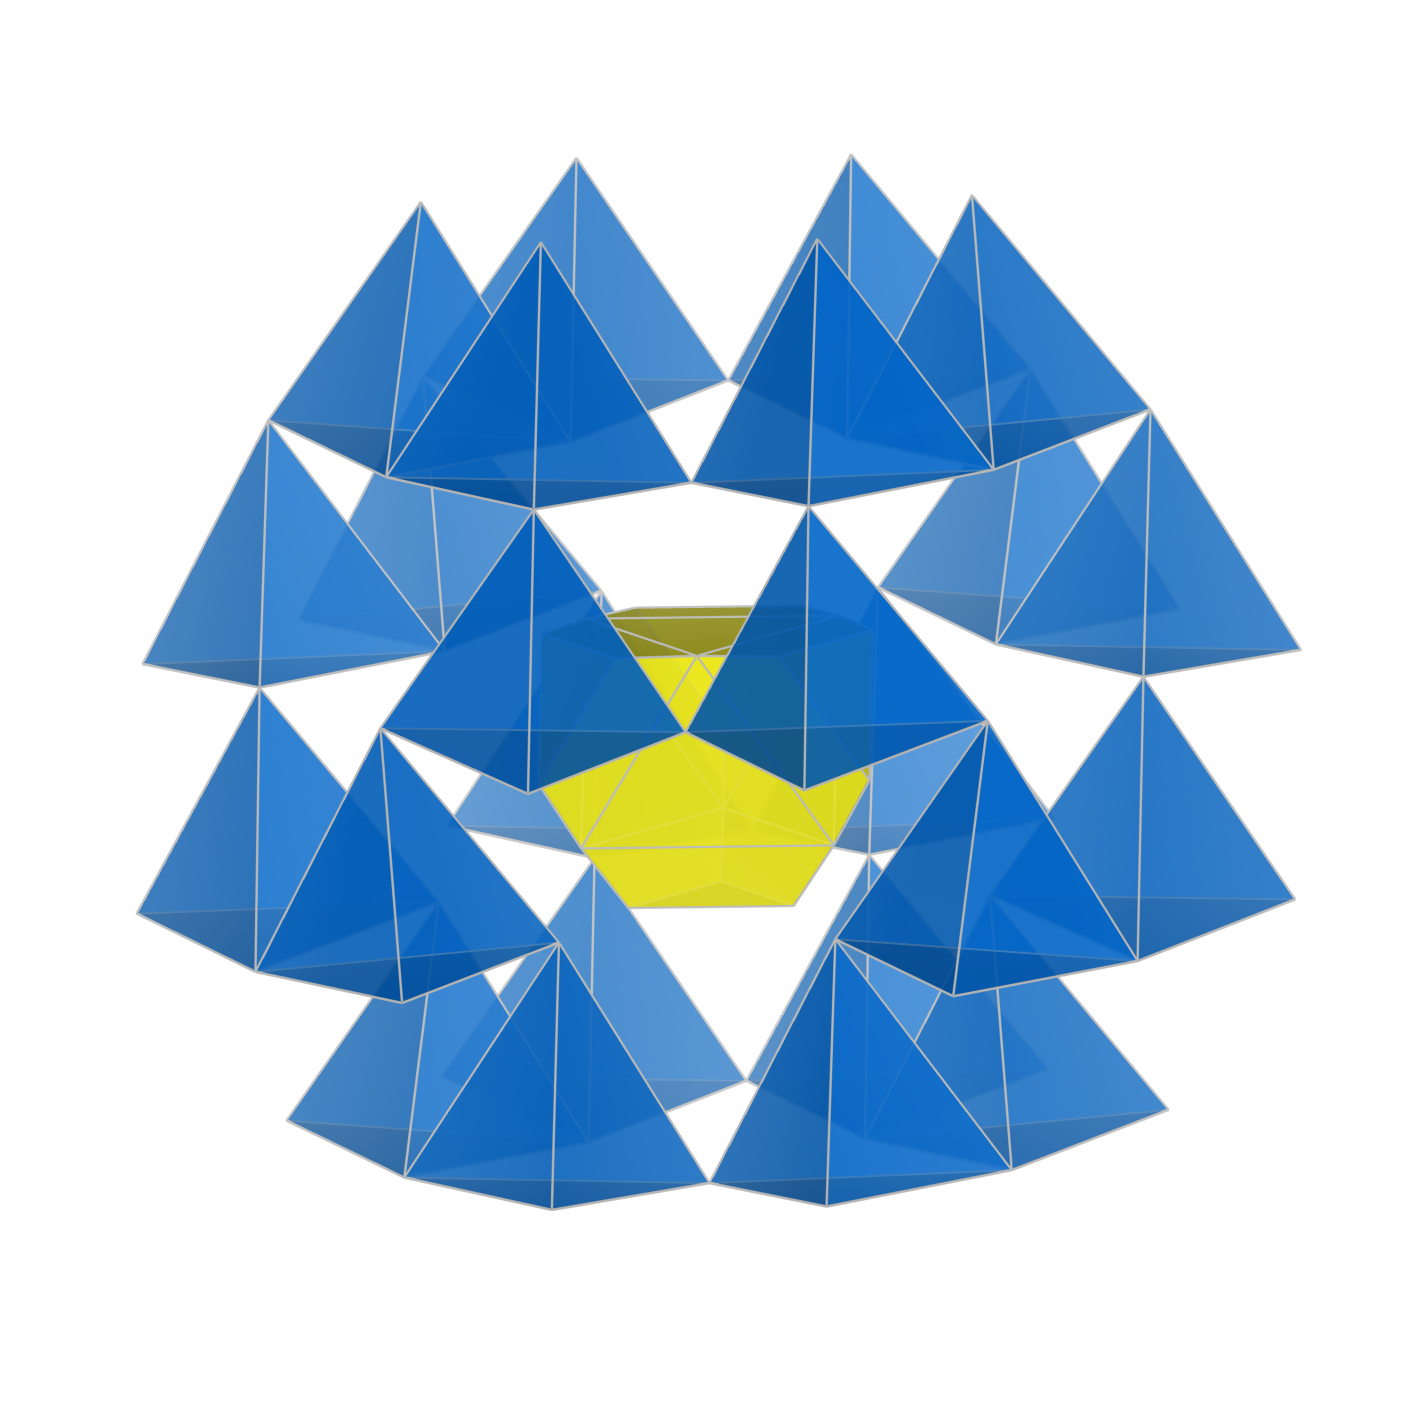
\includegraphics[width=0.6\linewidth]{2_cu12as4s13_crys_st_b} \\ а)
  \end{minipage}
  \vfill
  \begin{minipage}[ht]{0.99\linewidth}\centering
    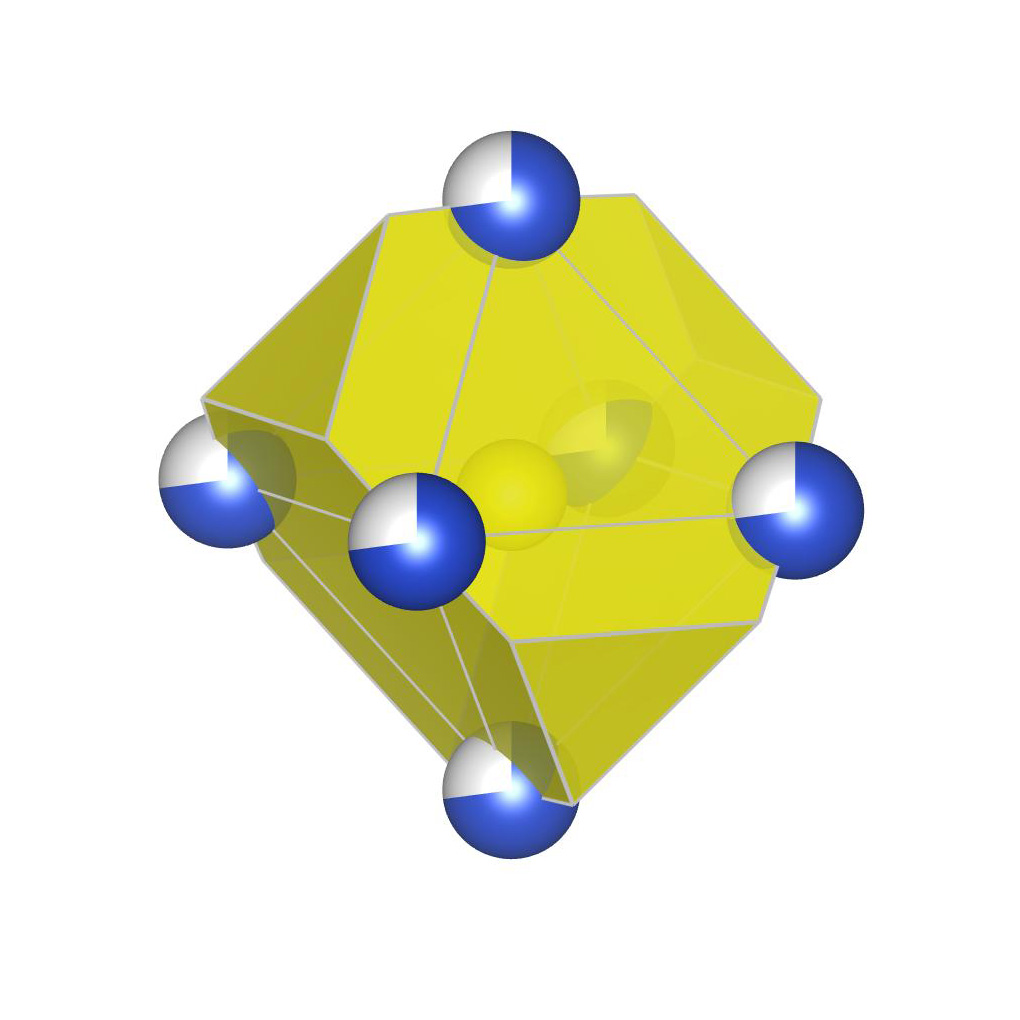
\includegraphics[width=0.6\linewidth]{3_cu12as4s13_crys_st_d} \\ б)
  \end{minipage}

      \caption[Кристаллическая структура халькогенида на примере синтетического теннантита Cu\textsubscript{12}As\textsubscript{4}S\textsubscript{13}]{Кристаллическая структура халькогенида на примере синтетического теннантита Cu\textsubscript{12}As\textsubscript{4}S\textsubscript{13}}
    \label{img:figure1}
\end{figure}

Структуры соединений тетраэдрита и теннантита являются близкими к структурам сфалерита или халькопирита\cite{Pauling1934}.
Если увеличить структуру сфалерита ZnS вдвое по ребру, то элементарная ячейка будет содержать в восемь раз больше атомов: 32 катиона Zn\textsuperscript{2+} и 32 аниона S\textsuperscript{2+}. Заменяя часть металлических катионов Zn\textsuperscript{2+} катионами полуметалла X\textsuperscript{3+} и оставляя часть катионов одновалентными X\textsuperscript{+}, получаем состав A$^{+}_{24}$X$^{3+}_{8}$S$^{2-}_{32}$. Удаление восьми анионов S\textsuperscript{2-} создает характерные для тетраэдрита комплексы полуметаллов [X$^{3+}$S$^{2-}_{3}$]. Получившиеся элементы пространства образуют форму тетраэдров, соответствующую пустым октантам сфалеритовой ячейки. На месте восьми анионов S\textsuperscript{2-} находятся атомы полуметалла  X\textsuperscript{3+}, которые создают  электронные пары. Таким образом, получается, что половина всех ионов A\textsuperscript{+} вблизи тетраэдров находится без полноценного окружения, координация по анионам S\textsuperscript{2-} равна двум, координация полуметаллов трём. Другая половина ионов A\textsuperscript{+} обладает четверной координацией, которая осталась как у сфалерита. Далее в центр из двух пустых тетраэдров обратной ориентации, где находятся неподелённые электронные пары, вводится дополнительный анион S\textsuperscript{2-}. Введение дополнительного аниона повышает S\textsuperscript{2-}  координацию половины атомов A\textsuperscript{+} до трех. После введения 2S\textsuperscript{2-} необходимо скомпенсировать заряд катионной части на четыре единицы, для чего четыре трёхкоординированных катиона A\textsuperscript{+} заменяются на A\textsuperscript{2+}. Получается, что общий состав тетраэдрита может быть выражен

\begin{equation}
  \label{eq:equation3}
  A^+_{20}A^{2+}_4[X^{3+}S^{2-}_{3}]^{3-}_{8}S_2.
\end{equation}



В литературе широко обсуждаются возможные методы построения структуры тетраэдрита. Авторы \cite{Koch_1981} рассматривают структуру тетраэдритов на основе кубически инвариантного комплекса  \textit{W*}. Этот комплекс находится около идеальных тетраэдров и обладает с ними общими вершинами.
Авторы статьи детально обсуждают соединения тетраэдрита и теннантита с точки зрения гомогенных или негомогенных структур в контексте W*(4t\textsubscript{c}) и (F$^{''}_{2}$-I(4t)) решеток.
Если рассматривается структура W*, то возможная максимальная симметричная группа для этой структуры~--- Im3m. В этом случае вершины располагаются в позиции 24(h) xx0 с $x = \frac{1}{4}\sqrt{2} = 0.3536$, центры этих вершин будут располагаться в 12(d) $\frac{1}{4}\frac{1}{2}0$.
В настоящее время таких структур не найдено, что оставляет открытым вопрос расположения атомов в элементарной ячейке тетраэдрита.
Также известно, что значение  z в позиции 24(g) xxz для силикатных структур лежит в диапазоне 0.025~$<$~z~$<$~0.085, в то время как этот же параметр для соединений со структурой тетраэдрита лежит в диапазоне 0.135~$<$~z~$<$~0.165.
Исходя из описанного выше, авторы приходят к мнению, что соединения из группы тетрадаэдрита и теннантита, относящиеся к I$\overline{\!4}$3m, могут быть описаны двумя разными гомогенными решетками W*(4t\textsubscript{c}) и (F$^{''}_{2}-$I(4t)), наследованными от силикатных структур.


Авторами работы \cite{Johnson1986} рассмотрено 1271 образцов натурального  и 295 синтетических образов тетраэдрита. Данная работа проведена с целью изучения механизмов замещения элементов Ag, Fe, Zn, Hg, Cd, As, Te, Bi в структуре тетраэдрита. Исследование показало, что на структурную формулу могут приходиться от четырех до десяти атомов Cu,  до четырех атомов Ag и не более двух атомов Fe, Zn, Hg. Возможно полное замещение между атомами As и Sb при неизменном составе атомов S в элементарной ячейке.
По данным авторов, описать замещение атомами Pb, Bi и Cd не представлялось возможным ввиду малого количества данных. Структуры с замещенными атомами Co, Ni, Mn и Au не обнаружены. Предложена общая формула (Cu,Ag)\textsubscript{6}Cu\textsubscript{4}(Fe,Zn,Cu,Hg,Cd)\textsubscript{2}(As,Sb,Bi,Te)\textsubscript{4}(S,Se)\textsubscript{13}. Размер элементарной ячейки возрастает с увеличением атомного номера допируемых элементов, за исключением тетраэдритов содержащих Ag. Атомы Ag и As обладают низкой тенденцией к взаимодействию, что подтверждается графиками замещения для Fe от As, Zn от Ag, Hg от Cu. Для объяснения этих механизмов используется модель предложенная Джонсоном \cite{johnson1983brillouin}. Эта модель заключается в анализе распределения заряда свободных электронов в структуре. Анализ показывает, что структура предсказывает наличие соединений со структурными формулами  Cu\textsubscript{14}Sb\textsubscript{4}S\textsubscript{13}~--- Cu\textsubscript{12}Sb\textsubscript{4.67}S\textsubscript{13}.

Этими же авторами \cite{Johnson1988} обсуждается кристаллохимия тетраэдритов, и предлагается общая формула \textsuperscript{IV}M(I)\textsubscript{6}\textsuperscript{III}M(II)\textsubscript{6}[\textsuperscript{III}X\textsuperscript{IV}Y\textsubscript{3}]\textsuperscript{VI}Z\textsubscript{4} (M(1) $=$ Cu, Fe, Zn, Mn, Hg, Cd; M(2) $=$ Cu, Ag; X $=$ Sb, As, Bi, Te; Y и Z $=$ S,Se)  для описания структуры тетраэдрита. Эта структура вводится по аналогии с содалитовой структурой с тетраэдрами M(1)Y\textsubscript{4}, которые содержат октаэдры ZM(2)\textsubscript{6}. Такое описание структуры приводит к увеличению связей между M(1)--Y и X--Y. Искажение решетки тетраэдра обуславлено влиянием изменения длины связи M(1)--Y и более сильным влиянием от изменения связи X--Y. Также отмечается влияние температуры и давления синтеза на кристаллографические особенности соединений. В заключении работы авторы делают вывод, что предложенная модель имеет ограничения при построении диаграммы P--T--X и необходимы дальнейшие исследования.

Вариации строения кристаллической структуры и полиморфизм в системе Cu--Sb--S при температуре ниже 400\textsuperscript{$\circ$}С рассматривается в исследовании \cite{Tatsuka_1977}. Основной результат работы заключается том, что тэтраэдрит стабилен при температуре 95\textsuperscript{$\circ$}С со структурной формулой Cu\textsubscript{12+x}Sb\textsubscript{4+y}S\textsubscript{13}, где 0.11~$\leqslant$~X~$\leqslant$~1.77 и 0.03~$\leqslant$~Y~$\leqslant$~0.3. Авторы установили, что ниже 95\textsuperscript{$\circ$}С соединение тетраэдрита образует две несмешиваемых фазы, которые описываются структурой тетраэдрита. Образование фаз быстрое и обратимое. Исследования структуры получившихся фаз показывают, что различие структуры двух фаз заключается в особенностях распределений позиций меди. Трансформация из одной фазы в другую происходит даже при добавлении лишнего атома меди или серы, в том числе и при комнатной температуре. Отмечается, что при комнатной температуре могут обнаруживаться фазы со структурными формулами Cu\textsubscript{12}Sb\textsubscript{4}S\textsubscript{13} и Cu\textsubscript{14}Sb\textsubscript{4}S\textsubscript{13}. Две эти фазы образуются на основе Cu\textsubscript{3}Sb\textsubscript{0,99}S\textsubscript{3}, с параметром ячейки a~$=$~20.848~$\pm$~0.006~$\angstrom$ и имеют название псевдотетраэдрит. Фаза псевдотетраэдрита стабильна до 350\textsuperscript{$\circ$}С и при более высокой температуре трансформируется в фазы тетраэдрита. Выше температуры 361\textsuperscript{$\circ$}С появляется высокотемпературная фаза Cu\textsubscript{3}SbS\textsubscript{3}. Превращение из фазы Cu\textsubscript{12}Sb\textsubscript{4}S\textsubscript{13} в Cu\textsubscript{14}Sb\textsubscript{4}S\textsubscript{13} и обратно объясняется мобильностью атомов меди в структуре.

На особенности формирования фаз система Cu--As--S исследовалась методами дифференциального термического и рентгенофазового анализов в работе \cite{Kurz_1989}. Установлено наличие квазибинарных соединений Cu\textsubscript{2}S--As, As--Cu\textsubscript{3}AsS\textsubscript{3}, Cu\textsubscript{3}S--Cu\textsubscript{2}S и Cu\textsubscript{2}S--As\textsubscript{2}S\textsubscript{3}. Также обнаружено два близких соединения Cu\textsubscript{6}As\textsubscript{4}S\textsubscript{9} и Cu\textsubscript{4}As\textsubscript{2}S\textsubscript{5}. Данные соединения и Cu\textsubscript{24}As\textsubscript{12}S\textsubscript{31} относятся к структуре производной от сфалеритовой, и находятся в области гомогенности соединения Cu\textsubscript{4}As\textsubscript{2}S\textsubscript{5} на фазовой диаграмме для системы  Cu--As--S. Отмечается наличие двух модификаций для соединения Cu\textsubscript{3}AsS\textsubscript{3}, низкотемпературная фаза которого известна как теннантит. Высокотемпературная фаза получается закалкой. Некоторые данные показывают, что соединения Cu\textsubscript{5}AsS\textsubscript{4} подобны минералу стефаниту Ag\textsubscript{5}SbS\textsubscript{4}. Соединения получены спеканием в кварцевых ампулах в вакууме. Часть структурных исследований была проведена на монокристальном дифрактометре Enraf--Nonius CAD 4. В настоящей диссертационной работе детально описываются особенности получения описанных выше фаз.

В статье \cite{Makovicky1995} обсуждается полиморфная фаза Cu\textsubscript{3}SbS\textsubscript{3}. Автором предложена модель  структуры в триклинной сингонии (группа симметрии P2\textsubscript{1}/c). Параметры ячейки a~$=$~7.814(1)~$\angstrom$, b~$=$~10.242(1)~$\angstrom$, c~$=$~13.273(1)~$\angstrom$, $\beta$~$=$~90.29(1)\textsuperscript{$\circ$} c Z~$=$~8. Атом Sb находится в треугольной пирамидальной координации в окружении призм, созданных вследствие двойникования из-за ряда атомов~S ((11$\overline{\!2}$2)\textsubscript{hcp}). Длина связи Sb--S лежит в диапазоне от 2.26 до 2.47~$\angstrom$. Большинство атомов в позиции Cu обладают тройной координацией с длиной связи для Cu--S в диапазоне от 2.26 до 2.31~$\angstrom$. Позиция Cu4 обладает тройной или четверной координацией с длиной связи для Cu--S в диапазоне от 2.40 до 2.46~$\angstrom$. Отмечается, что P2\textsubscript{1}/c--скиннерит является низкотемпературной модификацией Cu\textsubscript{3}SbS\textsubscript{3}. Разница в особенностях расположения атомов меди в структурах P2\textsubscript{1}/c--скиннерит и P2\textsubscript{1}2\textsubscript{1}2\textsubscript{1}/c--виттихенит связывается с различным размером полиэдров Sb и Bi соответсвенно.

Авторами \cite{Pfitzner1998a} продолжена классификация фаз соединения Cu\textsubscript{3}SbS\textsubscript{3}. Определена кристаллическая структура $\alpha$--Cu\textsubscript{3}SbS\textsubscript{3} при 493 К и 403 К методами монокристальной дифрактометрии. Высокотемпературная фаза, которая стабильна при температурах выше 394~К, кристаллизуется в орторомбическую кристаллическую решётку: параметры ячейки a~$=$~7.808(1)~$\angstrom$, b~$=$~10.252(2)~$\angstrom$, c~$=$~6.587(2)~$\angstrom$,  c Z~$=$~4, группа симметрии P\textsubscript{nma} (номер 62). Для данного соединения определено распределение атомов меди в тетраэдре [SbS\textsubscript{3}]\textsuperscript{3-}.  Атомы меди располагаются между пятью позициями с тройной или четверной координацией и пустых октаэдров S\textsubscript{6}.  Методами порошковой дифрактометрии при температуре 223~K определена кристаллическая структура $\gamma$--Cu\textsubscript{3}SbS\textsubscript{3}. Низкотемпературная фаза кристаллизуется в орторомбическую кристаллическую решётку: параметры ячейки a~$=$~7.884(1)~$\angstrom$, b~$=$~10.221(1)~$\angstrom$, c~$=$~6.624(1)~$\angstrom$,  c Z~$=$~4, группа симметрии P2\textsubscript{1}2\textsubscript{1}2\textsubscript{1}. Исследованные образцы получены спеканием в эвакуированных ампулах из соединений Cu\textsubscript{2}S и Sb\textsubscript{2}S\textsubscript{3} при температуре 853~К. Методика получения описана в работе \cite{Pfitzner_1994}. Отмечается, что структура высокотемпературной фазы определена на образце,  который использовался для определения структуры фазы $\beta$--Cu\textsubscript{3}SbS\textsubscript{3}. Обработка данных с монокристального эксперимента проводилась в JANA96, а с порошкового~---~в FULLPROF. Авторы отмечают, что структура для $\gamma$--Cu\textsubscript{3}SbS\textsubscript{3} получена методом Ритвельда с начальной структурой Cu\textsubscript{3}BiS\textsubscript{3}. Размер параметра кристаллической решетки для Cu\textsubscript{12}Sb\textsubscript{4}S\textsubscript{13} при температуре 223~К брался для определения особенностей структуры Cu\textsubscript{12+x}Sb\textsubscript{4}S\textsubscript{13}. Далее авторы проводят рассуждения о возможных вариантах расположения атомов меди в структуре, основываясь на  функции распределения электронной плотности. Атомы меди в позиции Cu(1) и Cu(2) находятся вне октаэдров S\textsubscript{6}. Атом меди в позиции Cu(3) располагается на гранях октаэдра  S\textsubscript{6}. Отмечается, что расстояние между атомами в позиции Cu(1) и Cu(2)~---2.099(9)~$\angstrom$, между  Cu(1) и Cu(3)~---1.266(9)~$\angstrom$, а между Cu(2) и Cu(3)~---1.93(1)~$\angstrom$. Полученные данные говорят о возможном нахождении атомов меди во всех трех позициях Cu(1), Cu(2) и Cu(3). Также авторы замечают, что структура Cu\textsubscript{3}SbS\textsubscript{3} не может быть описана в моноклинной сингонии. Высокотемпературная модификация имеет разориентировку как минимум вокруг пяти различных позиций, а уменьшение расстояния между атомами меди, необходимое для возникновения связи d\textsuperscript{10}--d\textsuperscript{10} оболочек путём введения дополнительного атома меди и аниона, может привести к появлению сверхрешётки, но дальнейших данных по этому предположению в статье нет.


В работе \cite{Makovicky2005} представлено первое исследование структуры монокристаллического образца минерала теннантит. Формула теннантита по результатом исследования авторов является Cu\textsubscript{12.5}As\textsubscript{0.98}Sb\textsubscript{0.02}S\textsubscript{13}. Исследование проведено на образце с линейными размерами 108$\times$72$\times$54~мкм\textsuperscript{3} при комнатной температуре и Mo K\textsubscript{$\alpha$} излучении на дифрактометре Bruker SMART CCD. Параметры ячейки определены по 1068 рефлексам (I~$>$~8$\sigma$\textsubscript{I}) с помощью программного обеспечения SMART и SAINT. Образец проиндицирован в кубической сингонии I$\overline{\!4}$3m с размером ребра кристаллической ячейки 10.1756(9)~$\angstrom$ c R--фактором 0.072. Авторы отмечают, что основная часть позиций атомов полностью заселена и являлась фиксированной при дальнейшем уточнении структуры. Обнаружено, что позиции меди Cu2A и Cu2B не полностью заселены, и установлена корреляция между фактором смещения и заселенностью атомов в этих позициях. Между двумя атомами в позиции Cu2B находится один атом в позиции Cu2A, такое расположение образует ярко выраженные эллипсоиды, расположенные вдоль линии, соединяющей Cu2A и Cu2B.  По мнению авторов, такое расположение атомов подтверждает возможное статистическое распределение и движение атомов меди  по этим позициям. Заселенность позиций атомов Cu2A и Cu2B составляет 75 и 17~\% соответственно. Таким образом, почти в каждой позиции Cu2A находится атом меди. Данные структурного и химического анализа показывают, что могут существовать ситуации, при которых два атома меди будут находиться в позиции  Cu2B. Авторы отмечают, что проводили уточнение структуры в группе симметрии P1 и утроенной элементарной ячейки, и получили тот же результат, что и при уточнении в кубической симметрии. Рассуждения о частичной заселенности показывают, что в структуре не может находится вакантных позиций в лавесовском полиэдре.



В работе \cite{Nasonova2016} исследована структура низкотемпературной фазы синтетического тетраэдрита Cu\textsubscript{12}Sb\textsubscript{4}S\textsubscript{13}. Структура соединения получена методами порошкового рентгенофазового анализа в диапазоне температур от 10 до 293 К. Установлено, что при температуре около 90 К происходит фазовый переход типа металл--полупроводник,  смещение атома серы вдоль поверхности октаэдра Cu\textsubscript{6} и сдвиг атома меди вдоль треугольника S\textsubscript{3}, которые связаны с двумя независимыми позициями атомов серы и резким увеличением расстояния между Cu--Sb. Отмечается, что фазовый переход значительно влияет на транспортные свойства соединения: зарегистрировано резкое возрастание электрического сопротивления. Предположение о предсказании сверхструктуры не подтверждено \cite{Tanaka2015}.
Низкая теплопроводность, по мнению авторов, является следствием наличия квазилокализованных атомов меди, которые приводят к размягчению кристаллической решетки с повышением температуры.
Исследуемые образцы синтетического тетраэдрита были получены стандартным ампульным методом в стехиометрическом соотношении 12:4:13 в кварцевых ампулах под давлением 2$\times$10\textsuperscript{-2}~Торр. Ампулы нагревались до 973~К и отжигались в течение трех часов при этой температуре, после медленно охлаждались до 823~К в течение 30 часов, остывали при выключенной печи до комнатной температуры. Полученные спёки перетерались в агатовой ступке и были спресованы в таблетки под давлением 80--100~бар при комнатной температуре. Полученные таблетки отжигались в вакуумированных ампулах при 773~К в течение 25~часов. Структурные исследования были проведены на канале ID22 Европейского синхротронного источника с энергией $\lambda$~=~0.41066~$\angstrom$, с шагом 10~К в диапазоне температур от 10 до 150~К и с шагом 15~К в диапазоне температур от 150 до 240~К. Авторы отмечают, что все позиции атомов серы в соединениях Cu\textsubscript{12}Sb\textsubscript{4}S\textsubscript{13} и Cu\textsubscript{12}Sb\textsubscript{4}S\textsubscript{12.8} полностью заселены, за исключением позиции Cu(2). Для этих соединений установлены различные коэффициенты атомарных смещений 0.0102(4) и 0.0125(3) для позиции атома S(1), 0.016(2) и 0.019(2) для позиций атома S(2) и размер ребра элементарной ячейки 10.33051(2) и 10.33344(1)~$\angstrom$ соответсвенно для Cu\textsubscript{12}Sb\textsubscript{4}S\textsubscript{13} и Cu\textsubscript{12}Sb\textsubscript{4}S\textsubscript{12.8}. Ввиду близкого расположения позиций атомов Cu(2) для уточнения структуры при низких температурах взята структура Cu\textsubscript{12}Sb\textsubscript{4}S\textsubscript{13}  при комнатной температуре. С понижением температуры до фазового перехода кристаллическая ячейка уменьшается, но после фазового перехода размер кристаллической ячейки перестает уменьшаться с понижением температуры и показывает локальный максимум при 40~К. Этот фазовый переход вызван изменением положения атомов в позиции Cu(2). Так, максимальное и минимальное расстояние между позициями атома Cu(2) изменяется в три раза, а максимальное расстояния между позициями атомов Cu(2) и Sb(1) возникает при температуре соответствующей локальному максимуму размера кристаллической ячейки при 40~К. Ниже температуры фазового перехода возникает волна зарядовой плотности (или упорядочение зарядов Cu\textsuperscript{$+$}Cu\textsuperscript{$2+$} на атомах меди) за счет изменения позиций атомов меди Cu(2). Авторами исследованы транспортные свойства полученных соединений. Благодаря полученным ими данным была найдена характеристическая температура Дебая, возникающая ввиду наличия квазилокализованных фононных мод в кристаллической решетке. Авторы отмечают, что полученные ими данные для характеристических температур Эйнштейна отличаются от опубликованных в литературе данных\cite{Lara-Curzio2014}.

В работе \cite{Friese2008} проведено исследование синтетических тетраэдрита и теннантита, доппированного железом при температурах 25 и 250\textsuperscript{$\circ$}С. Исследованные соединения обладают структурной формулой Cu\textsubscript{12-x}Fe\textsubscript{x}(As,Sb)\textsubscript{4}S\textsubscript{13}, где  x~$=$~0.10 и 1.23 для теннантита  и  x~$=$~0.61 и 1.83~Fe для тетраэдрита.
 Увеличение количества атомов железа в структуре и теннантита, и тетраэдрита приводят к увеличению расстояния между Cu1--S и Cu2--S, где Cu1~---~позиция замещения для атома Fe. Позиция Cu2 определена как сдвоенная позиция. Расстояние Cu2--Cu2 составляет 0.56 и 0.65~$\angstrom$ для тетраэдрита и теннантита соответсвенно. С увеличением температуры параметр ребра кристаллической решетки увеличивается на 0.02--0.04~$\angstrom$, а в среднем межатомное расстояние увеличивается на 0.01~$\angstrom$. Полученное значение коэффициентов термического расширения для доппированных соединений такое жк, как и для недоппированных.
 В работе авторы детально обсуждают особенности распределения меди. Отмечается, что наблюдается смещение центра позиции Cu2 с повышением температуры. Расстояние Cu2--Cu2 в доппированных соединениях принимает типичное для сульфосолей расстояние при температуре 250\textsuperscript{$\circ$}С. Особенности распределения меди в тетраэдрите и теннантите разные:
межплоскостная плотность в теннантите выше, чем в тетраэдрите. Определенная разница в кристаллографических особенностях для исследованных образцов объясняется уменьшением зарядовой плотности в лавесовском полиэдре.
\newpage

\section{Структурные особенности соединений Cu\textsubscript{3}AsSe\textsubscript{3} и Cu\textsubscript{3}SbSe\textsubscript{3}} \label{sect1_2}

Данные о кристаллической структуре Cu\textsubscript{3}AsSe\textsubscript{3} и Cu\textsubscript{3}SbSe\textsubscript{3} в литературе немногочисленны.

Впервые минерал мгриит (Cu, Fe)\textsubscript{3}AsSe\textsubscript{3} описан в работе \cite{Dymlcov_1983}. Исследуемый образец представлял из себя шлиф породы, в котором обнаружены вкрапления исследуемой фазы. Твердость исследуемого образца была в диапазоне от 287 до 379~кг/мм\textsuperscript{2}. Для сравнения: твердость теннантита лежит в диапазоне от 350 до 425~кг/мм\textsuperscript{2}. Количественный элементный анализ выявил формулу Cu\textsubscript{2.92}Fe\textsubscript{0.16}As\textsubscript{0.98}Se\textsubscript{2.96}. Рентгеноструктурный анализ проведен на характеристическом излучении Fe k\textsubscript{$\alpha$} на образцах диаметром 0.2 и 0.3~мм. Соединение обладает кубической сингонией и относится к группе симметрии Pd3M с параметром решетки a~$=$5.530$\pm$0.005~$\angstrom$, V~$=$169.48$\pm$0.005~$\angstrom^{3}$. Расчётная плотность составила 4.9~г/см$^{3}$.

В работе \cite{Majid_1987} рассмотрены трёхкомпонентные соединения, которые образуются в системе Cu--As\textsubscript{2}Se\textsubscript{3}. Основные результаты представлены в таблице \ref{tbl2}. Все соединения проиндицированы в кубической сингонии. Исследуемые образцы получены из особо чистых компонент в стехиометрическом соотношении ампульным методом.

\begin{table} [htbp]%
    \centering
	\caption{Сводная таблица кристаллических фаз, образованных в системе Cu--As\textsubscript{2}Se\textsubscript{3}\cite{Majid_1987}}%
	\label{tbl2}% label всегда желательно идти после caption
    \renewcommand{\arraystretch}{1.5}
	\begin{tabular}{@{}@{\extracolsep{20pt}}llll@{}}
        \toprule     %%% верхняя линейка
    	Соединение& Параметр эл. яч., $\angstrom$&Объем эл. яч., $\angstrom^{3}$& Плотность, г/см\textsuperscript{3}	\\
        \midrule
    	Cu\textsubscript{3}AsSe\textsubscript{2} 	& 5.513$\pm$0.004	 & 167.47												&5.88	\\ \hline
    	Cu\textsubscript{3}AsSe\textsubscript{4} 	& 5.530$\pm$0.005	 						& 169.11												&5.75		\\ \hline
    	Cu\textsubscript{3}AsSe\textsubscript{3} 	& 5.758$\pm$0.009	 						& 190.87												&4.45		\\ \hline

        \bottomrule
	\end{tabular}%
\end{table}

В статьях \cite{39_Demb_1970,40_Demb_1971} опубликованы результаты исследования твердых растворов в системе Cu\textsubscript{2}Se\textsubscript{3}--As\textsubscript{2}Se\textsubscript{3}. Отмечается, что в исследуемых твёрдых растворах при температуре 733~К образуется соединение Cu\textsubscript{3}AsSe\textsubscript{3}. Предполагается, что структура соединения обладает тетрагональной симметрией.
В работе \cite{39_Demb_1970} подробнее исследовалась система Cu\textsubscript{2}Se\textsubscript{3}--As\textsubscript{2}Se\textsubscript{3}. Результаты исследования показывают, что соединение Cu\textsubscript{3}AsSe\textsubscript{3} существует в интервале температур от 696 до 769~К, и реакция эвтектического распада медленно происходит  при температуре 393~К. В работе \cite{bab_1982} соединение Cu\textsubscript{3}AsSe\textsubscript{3} проиндицировано в кубической сингонии с параметром решетки a~$=$10.11$\pm$0.01~$\angstrom$.


В работе \cite{31_Whitfield_1980} описано соединение Cu\textsubscript{3}SbSe\textsubscript{3}. Исследуемый образец получен спеканием соединений Cu\textsubscript{2}Se и Sb\textsubscript{2}S\textsubscript{3} в стехиометрических пропорциях ампульным методом при температуре 720~К в течение 48~часов. После обжига полученный образец был закалён при T~$=$273~K в воде со льдом. Соединение обладает ромбической структурой и пространственной группой P\textsubscript{nma} с параметрами элементарной ячейки a~$=$7.97~$\angstrom$, b~$=$10.61~$\angstrom$ и c~$=$6.83~$\angstrom$, которая аналогична структурам соединений,  Cu\textsubscript{3}SbS\textsubscript{3} и  Cu\textsubscript{3}BiS\textsubscript{3}.


Отдельно стоит отметить, что широко обсуждаются механизмы и условия синтеза сложных халькогенидов. Основные результаты представлены в работах \cite{Sis_Frost2002,sis_karup59new,sis_Mueller2002,sis_Mueller2003,sis_Raghavan2004,sis_seal1990tetrahedrite,sis_Skinner1972,sis_Taras_Bryndzia_1988,sis_Tomkins2006,sis1_1347-4065-8-4-443,sis1_BALAZ1995375,sis1_Braga2008,sis1_Pfitzner:se0205,sis1_WELLER2017794}.
\newpage


\section{Физические свойства трёхкомпонентных соединений меди} \label{sect1_3}

Термоэлектрические и магнитные свойства в сложных халькогенидах связываются с особенностью распределения меди в <<лавесовских полиэдрах>>  и разориентировкой тетраэдрических комплексов в структуре. Так, например, аномально низкая теплопроводность связывается с ангармоническими тепловыми колебаниями в позиции атомов меди\cite{Mishra2017}, которые обуславливают аномально низкую теплопроводность. А изменение электронной структуры и, как следствие, изменение магнитных свойств, связываются с трансформацией комплексов  Cu\textsubscript{6}(S,Se)\textsubscript{12} при понижении температуры\cite{Gainov2008}. В тоже время опубликованные данные о механизмах формирования физических свойств различны, существует несколько мнений о механизмах низкотемпературных фазовых превращений.


В статье \cite{Lai_2015} обсуждается связь влияния особенностей распределения меди в кристаллической структуре тетраэдрита Cu\textsubscript{12}Sb\textsubscript{4}S\textsubscript{13} или (Cu12d)\textsubscript{12}(Cu12e)\textsubscript{12}(Sb8c)\textsubscript{8}(S2a)\textsubscript{2}(S24g)\textsubscript{24} на его транспортные свойства. Показана связь между локальной асимметрией связей и термоэлектрическими свойствами.
По мнению авторов, локальная асимметрия связей создаёт дополнительные связи, которые выявлены в пятиатомной структуре Sb[CuS\textsubscript{3}]Sb. Такие ассиметричные связи способствуют появлению мод, которые квазилокализованы и ангармоничны и обладают низкой фононной частотой и большой амплитудой. Подобные связи объясняют природу низкой теплопроводности в тетраэдритах. Авторы отмечают, что энергия таких мод составляет $\approx$~4 мэВ, что соответсвует волновому числу 33~см\textsuperscript{-1}.

Авторы работы \cite{Lara-Curzio2014} рассматривают особенности теплоёмкости в натуральных и синтетических образцах тэтраэдритов. Теплоёмкость природных  Cu\textsubscript{12$-$x}(Fe,Zn,Ag)\textsubscript{x}(Sb,As)\textsubscript{4}S\textsubscript{13} и синтетических Cu\textsubscript{12$-$x}Zn\textsubscript{x}(Sb,As)\textsubscript{4}S\textsubscript{13}, при x~$=$~0,1,2, образцов измерена в диапазоне от 2 до 380~К. Установлено, что полученные зависимости теплоёмкости хорошо описываются моделью Дебая с тремя дополнительными осцилляторами Эйнштейна 12, 32.5 и 97~К соответсвенно. Предполагается, что осцилляторы Эйнштейна появляются ввиду ангармонических тепловых колебаний атомов. Эти колебания возникают при нестабильном перекрытии d-орибитали Cu c p-орбиталью S.
Наличие осцилляторов Эйнштейна, которые обуславливаются ангармоническими тепловыми колебаниями атомов, уменьшает теплопроводность и, как следствие, улучшает термоэлектрические свойства.

В работе \cite{Gainov2008} рассматриваются электрические и магнитные свойства природного теннантита. Исследование проведено методом ядерного квадрупольного резонанса и методом измерения намагниченности в СКВИД магнетрометре. Авторы исследовали перескакивание спинов между комплексами CuS\textsubscript{3} через S\textsubscript{2}. Анализ полученных зависимостей показывает наличие фазового магнитного перехода около 65~К. Магнитная восприимчивость измерена в диапазоне от 2 до 300~К и имеет характерный вид для парамагнетика. Основной вклад в парамагнетизм внесен ионами Fe\textsuperscript{2+}. В обсуждении результатов отмечается высокая чувствительность метода к изоморфным аналогам. Определена энергия активации, которая составляет 65~К. Ниже этой температуры происходит <<вымораживание>> внутренних локальных флуктуаций, которые связываются с необычным поведением квадрупольной частоты меди. Авторами рассматривается вопрос о валентности атомов меди. Отмечается, что локальные флуктуационные поля от Cu\textsuperscript{1+} влияют на осцилляции Cu\textsuperscript{2+}, наиболее значимое влияние оказывают атомы первой координационной сферы. Тогда получается, что Cu\textsuperscript{2+} находятся в кластере Cu\textsubscript{6}S\textsubscript{13}. Это предположение вводится по аналогии с данными из работы\cite{Pattrick1993}, где кластер [Fe\textsubscript{3}S\textsubscript{4}]\textsuperscript{0} сравнивается с Cu\textsubscript{6}S\textsubscript{13} и предполагается наличие обменного взаимодействия.  Также рассматриваются деформация кристаллической структуры и изменение локального электронного окружения в контексте наличия эффекта Яна--Теллера, связанного с  Cu\textsuperscript{2+}.

Авторы работы \cite{DiBenedetto2002} провели исследование 130  природных образцов тетраэдритов из Природного музея Флоренции методами электронной растровой микроскопии, рентгенофазового порошкового анализа, дифференциального термического анализа, электронного парамагнитного резонанса и методом СКВИД магнитометрии. Исследования электронного парамагнитного резонанса и магнитной восприимчивости проведены на выборочных образцах. Во всех образцах найдено небольшое количество Cu\textsuperscript{2+} и Fe\textsuperscript{2+}. Fe\textsuperscript{3+} обнаружен только в дефектных образцах. Исследования электронного парамагнитного резонанса на отобранных образцах с высокой концентрацией Cu\textsuperscript{2+} показывают сильную анизотропию. Для объяснения анизотропии рассматривается модель несвязанных электронов двух парамагнитных центров, которые почти полностью делокализованы в направлении Cu--S--Cu. В данном направлении образуются мосты, которые в основном образованы p- и d-орбиталями\cite{Albright_2013}. Также рассматриваются зависимости обратной магнитной восприимчивости от температуры с учетом высокотемпературной магнитной модели Гейзенберга. Отмечается наличие антиферромагнитных взаимодействий, а также двухвалентность атомов железа, которые находятся в позициях тетраэдров. Авторы делают вывод, что атомы Cu\textsuperscript{2+}, находятся в образцах, где сумма катионов меньше 12, координационный полиэдр Cu\textsuperscript{2+} разориентирован, наличие взаимодействия между Cu\textsuperscript{2+} говорит о наличии димеров. Обнаружено наличие остаточной намагниченности при температурах ниже фазового перехода. При 4.2~К наблюдается наличие парамагнитных центров.  Измерения электронного парамагнитного резонанса проведены на спектрометрах Bruker~200D и Bruker~ESP380.

Продолжением предыдущей работы является статья \cite{DiBenedetto2005}, в которой исследуются магнитные свойства синтетического тетраэдрита Cu\textsubscript{12}Sb\textsubscript{4}S\textsubscript{13}. Синтетический тетраэдрит исследован методами измерения намагниченности, дифференциальной сканирующей калориметрии и импульсного электронного парамагнитного резонанса для получения данных о распределении атомов Cu\textsuperscript{2+}.
Сильное антиферромагнитное упорядочение, наблюдаемое при комнатной температуре, связано с фазовым переходом при 85~К. Авторами установлено, что атомы Cu\textsuperscript{2+} случайным образом расположены в позиции тетраэдрита M(1). По мнению авторов, такое расположение атомов меди в структуре создает антиферромагнитное взаимодействие. Исследуемые образцы были получены синтезом из бинарных соединений CuS, Cu\textsubscript{2}S, Sb\textsubscript{2}S\textsubscript{3} в среде KCl:LiCl при температуре 400\textsuperscript{$\circ$}С. Образцы аттестованы методам порошкового рентгеноструктурного анализа и анализом на элементный состав. Магнитная восприимчивость была измерена в диапазоне от 2 до 298~К на СКВИД магнитометре в режиме FC при постоянных магнитных полях 2 и 0.1~T. Теплоёмкость измерена на Quantum Design
PPMS в диапазоне температур от 75 до 100~К. В работе приводится литературный обзор по особенностям распределения меди в структуре тетраэдритов. График магнитной восприимчивости имеет отклонение в диапазоне температур от 60 до 100~К. Детальное исследование графика магнитной восприимчивости показывает, что фазовый переход проиходит между 79~К и 86~К. График зависимости теплоёмкости от температуры имеет вид почти линейной зависимости в диапазоне от 85 до 100~К. Полученные зависимости электронного парамагнитного резонанса показывают, что несвязанные электроны Cu\textsuperscript{2+} взаимодействуют с большим количеством протонов и с ядром Sb.



В работе \cite{Levinsky_2015} рассмотрены магнитные и термоэлектрические свойства четырех природных образцов из группы тетраэдрита--теннантита. Интерес к исследованию этих соединений вызван высоким потенциалом их использования как функциональных материалов для термоэлектрических устройств. Все образцы показывают p--тип проводимости с низкой мобильностью. Антиферромагнитное взаимодействие обусловлено наличием атомов Fe\textsuperscript{2+}. Максимальное значение ZT составляет 0.13 при температуре 700~K. Для измерения термоэлектрических свойств образцы были перетерты и дополнительно подготовлены методом плазменного спекания. Исследования магнитных свойств показывают, что  атомы железа в структуре могут находиться в качестве ферромагнитных атомов.

В работе \cite{Suekuni_2013} синтезированы  соединения Cu\textsubscript{12-x}Ni\textsubscript{x}Sb\textsubscript{4}S\textsubscript{13} (где x~$=$~0,~0.5,~1.0,~1.5 и 2.0), и проведено исследование термоэлектрических свойств. Авторы отмечают наличие низкоэнергетичных мод у атомов в позиции Cu(2) находящихся вне CuS\textsubscript{3}. Эти моды понижают теплопроводность ниже 0.5~В\textsuperscript{-1}м\textsuperscript{-1}. Допирование Ni приводит к возрастанию значения ZT. Максимальное значение 0.7 достигнуто при x~$=$~1.5 и температуре 665~К. Образцы были подготовлены ампульным методом. Шихты закладывались в стехиометрическом соотношении, нагревались в вакууме до температуры 973~К и выдерживались в течении 3 часов. Далее в течении 30 часов ампулы обжигались при температуре 823~К и остывали до комнатной температуры. Полученные образцы были измельчены и спрессованы в таблетки, которые обжигались в вакууме при температуре 773~К в течение 25 часов. Отожжённые образцы были повторно измельчены и спечены при температуре 803~К в течении одного часа в аргоне при давлении 60~МПа. Согласно данным рентгеноструктурного анализа атомы в позиции Cu(1) находились в тетраэдрах CuS\textsubscript{4}. Значение параметра кристаллической составляло от 10.319--10.323$\angstrom$, что хорошо согласуется с опубликованными ранее данными. Авторы детально рассматривают амплитуду тепловых колебаний атомов меди. По этой величине авторы определяют температуру Дебая, соответствующую этим колебаниям. Проведены оценки электропроводности по закону Видемана--Франца, из которых установлено, что наблюдается высокое рассеяние на фононах. В заключение авторы отмечают, что высокое значение ZT обеспечивается низким значением решеточной теплопроводности.

Работа \cite{Suekuni2012} посвящена исследованию влияния допирования атомами Mn, Fe, Co, Ni, Cu и Zn на термоэлектрические и магнитные свойства тетраэдрита Cu\textsubscript{12}M\textsubscript{2}Sb\textsubscript{4}S\textsubscript{13}.
Максимальное значение ZT достигается при допировании никелем и составляет 0.15 при температуре 340~К.
Образцы получены стандартным ампульным методов в вакууме. Шихта в стехиометрическом соотношении нагревалась до 973~К, охлаждалась до 823~К в течение 30~часов, после~---охлаждалась в печи до комнатной температуры.
Образцы получены с относительной плотностью 75--85~\%.
Сводные данные для соединений представлены ниже в таблице \ref{tbl1}.
Сделан вывод, что термоэлектрические свойства зависят не только от особенностей фононного рассеяния при внедрении атомов замещения, но также от изменения электронной структуры, которая меняется при допировании.
В заключение авторы отмечают, что термоэлектрические свойства соединения со структурой тетраэдрита чувствительны к допированию. Также эти соединения обладают низкой решеточной проводимостью, соединение синтетического тетраэдрита претерпевает фазовый переход металл--полупроводник при температуре 85~К и имеет аномальный гистерезис при 300~К.


\begin{table} [htbp]%
    \centering
	\caption{Сводная таблица термоэлектрических свойств допированных соединений на основе тетраэдрита\cite{Suekuni2012}}%
	\label{tbl1}% label всегда желательно идти после caption
    \renewcommand{\arraystretch}{1.5}
	\begin{tabular}{@{}@{\extracolsep{20pt}}llll@{}}
        \toprule     %%% верхняя линейка
    	Атом замещения, M& $\angstrom$&мкВ/(K$^2$$\cdot$м)& ZT	\\
        \midrule
    	Mn 	& 10.42(1)	 						& 88												&0.07	\\ \hline
    	Fe		& 10.38(1) 	 						& 7													& 0.01		\\ \hline
    	Co		& 10.35(1) 						   & 37												& 0.03		\\ \hline
    	Ni		& 10.31(1) 							 & 177												& 0.15		\\ \hline
     Cu		& 10.31(1) 							 & 374												& 0.13		\\ \hline
		Zn		& 10.38(1) 							 & 46												& 0.03		\\ \hline
        \bottomrule
	\end{tabular}%
\end{table}


В работе \cite{Lu2013} исследуется влияние допирования в позиции меди в тетраэдрите Cu\textsubscript{12-x}M\textsubscript{x}Sb\textsubscript{4}S\textsubscript{13}, где атомами замещения служат атомы Zn или Fe. Соединения, исследованные в работе, получены стандартным ампульным методом, последующим отжигом и горячим прессованием. При значении x в диапазоне от 0 до 1.5 в соединении Cu\textsubscript{12-x}Zn\textsubscript{x}Sb\textsubscript{4}S\textsubscript{13} электропроводность в соединениях составляет 10\textsuperscript{-5}~Ом$\cdot$м. При значении x равном 1.5 сопротивление возрастает на один порядок в сравнении с беспримесным образцом.  При значении x равном 2 соединение становится изолятором. Различия обусловлены тем, что в работе \cite{Suekuni2012} в исследованных соединениях была примесь другой фазы. Допирование атомами Zn приводит к значительному возрастанию коэффициента Зеебека. Также исследовано влияние допирования атомами Fe в соединении Cu\textsubscript{12-x}Fe\textsubscript{x}Sb\textsubscript{4}S\textsubscript{13}, где x~$=$~0.2,~0.5 и 0.7, на термоэлектрические свойства. Максимальное значение ZT равное 0.8 достигается при x~$=$~0.5. Отмечается, что сопротивление Cu\textsubscript{11}Zn\textsubscript{4}S\textsubscript{13} в три раза больше, чем у Cu\textsubscript{11}FeSb\textsubscript{4}S\textsubscript{13}. Это связано с различием валентности атомов Fe и Zn, которое приводит к изменению концентрации дырок в валентной зоне.

В работе \cite{Heo2014} исследуются тепловые и электрические свойства синтетического тетраэдрита Cu\textsubscript{12}Tn\textsubscript{2}Sb\textsubscript{4}S\textsubscript{13}, где Tn~$=$~Mn, Fe, Co, Ni, Zn и твердого раствора Cu\textsubscript{12-x}Mn\textsubscript{x}Sb\textsubscript{4}S\textsubscript{13}, где 0~$\leq$~x~$\leq$~2. Исследование проводено для определения термоэлектрической эффективности каждого из соединений. По результатом экспериментов установлено, что соединение Cu\textsubscript{12}Sb\textsubscript{4}S\textsubscript{13} обладает самым высоким значением фактора мощности ввиду высокого значения электрической проводимости. Максимальное значение термоэлектрической эффективности из серии соединений Cu\textsubscript{12}Tn\textsubscript{2}Sb\textsubscript{4}S\textsubscript{13} получено для структуры, допированной Mn, и составляет 0.8 при 575~К. Добавление одного атома  Mn на структурную формулу Cu\textsubscript{12}Sb\textsubscript{4}S\textsubscript{13} приводит к значению термоэлектрической эффективности равной 1.13 при 575~К.

Также рассматриваются термоэлектрические свойства для твердых растворов Cu\textsubscript{12}Sb\textsubscript{4}S\textsubscript{13-x}Se\textsubscript{x}, где x~$=$~0,~0.5,~1.0 и 2.0\cite{Lu2016}.
Данная работа направлена на исследование замещения анионов в структуре тетраэдрита.
В работе приведены расчёты методом теории функционала электронной плотности и проведено структурное исследование на линии 11BM  синхротронного источника третьего поколения в Аргоннской национальной лаборатории.
Расчёты показали, что атом Se должен внедряться в позицию 24g тетраэдра.
Допирование атомами Se приводит к уменьшению электрического сопротивления без уменьшения значения ZT.
При x~$=$~1 наблюдается возрастание на 30~\% тепловой мощности в сравнении с Cu\textsubscript{12}Sb\textsubscript{4}S\textsubscript{13}.
Методика получения соединений описана ранее в работах \cite{Lu2013,Lu_2013b,Lu_2013}. По расчётам один допирующий атом Se  добавляет общую энергию 20~мэВ на кристаллическую ячейку, два~--- 30~мэВ.
Допирование третьим атомом Se делает структурную ячейку нейтрально заряженной. Расчёты также предсказывают внедрение атома Se в позицию S(1) при комнатной температуре и выше.
Термоэлектрические свойства для всех образцов имеют одинаковый характер, который согласуется с ранее опубликованными данными.
Как отмечено выше, коэффициент ZT не изменяется несмотря на уменьшение сопротивления в образце.
Увеличение электропроводности наблюдается для соединений с  x~$=$~2 выше температуры 600~K. Особенности увеличения электропроводности выше температуры 600~K подтверждаются теоретическими расчётами.

Исследования ядерного магнитного резонанса, магнитной восприимчивости и проводимости синтетического тетраэдрита Cu\textsubscript{12}Sb\textsubscript{4}S\textsubscript{13} были проведены в работе \cite{Kitagawa2015} до давления 4 ГПа. При давлении выше 1 ГПа возникает магнитное упорядочение. Анализ данных проведен в предположении наличия одно- и двухвалентных атомов меди.


В работе \cite{Kosaka2017} представлено исследование влияния допирования синтетического тетраэдрита. Исследовано замещение в Cu\textsubscript{12-x}M\textsubscript{x}Sb\textsubscript{4}S\textsubscript{13}, атомами Mn, Fe, Co, Ni и Zn. Также исследовано влияние замещения на температуру фазового перехода металл-полупроводник. Кроме того, исследовано замещение атомами Ge и Sn при x~$\leq $~0.6. Показано, что фазовый переход предотвращается ввиду заполнения электронной оболочки меди, подтверждается внедрение допируемых атомов в <<лавесовский>> полиэдр. Внедрение четырёхвалентных атомов вместо одновалентной меди приводит к возрастанию термоэлектрической мощности и возникновению низкой теплопроводности материала. По результатам исследования максимальное значение термоэлектрической добротности составляет 0.65 при температуре 665~К, x~$=$~0.3~$-$~0.5 и при допировании Ge и Se.

Актуальный обзор статей, посвященных термоэлектрическим свойствам,  можно найти по ссылке \cite{Powella}. В работах \cite{ther_10.1007/s11664-016-4893-7,ther_10.1016/j.intermet.2016.08.003,ther_10.1016/j.jallcom.2017.01.187,ther_10.1039/C7RA02564E,ther_10.1039/C7TC00762K,ther_AENM:AENM201200650,ther_C5TC01636C,ther_C6DT00564K,ther_doi:10.1021/acs.chemmater.7b00891,ther_doi:10.1021/acs.inorgchem.7b02128,ther_doi:10.1021/acs.jpcc.7b02068,ther_doi.org/10.1016/j.jssc.2017.01.003,ther_GONCALVES2016209,ther_HARISH2016323,ther_JACE:JACE13838,ther_lu2014effect}  представлены исследования термодинамических свойств сложных халькогенидов при допировании и при разных условиях синтеза.
В работе \cite{Kehoe_2013} рассматривается возможность использования соединений Cu\textsubscript{3}MCh\textsubscript{3} (M~$=$~Sb, Bi; Ch~$=$~S, Se) в фотовольтаике. Проведено моделирование электрофизических свойств соединений.
\newpage

\section{Выводы по Главе 1} \label{sect1_4}

В главе дан обзор литературных данных по структурным, транспортным и магнитным свойствам соединений из группы тетраэдрита-теннантита. Проанализированы особенности строения теннантита и тетраэдрита.

Полиэдр сформирован 6 атомами меди, которые располагаются  в центре рёбер не усеченного тетраэдра.
Сформированный лавесовский полиэдр окружен тетраэдрическими комплексами, направленными в одну сторону.
В такой структуре тетраэдритов и теннантитов, ввиду ян-тейллоровского искажения,  наблюдается сдвиг атомов меди из идеального положения, который приводит к  перекрытию электронных орбиталей атомов меди и формирует особенную электронную структуру.
Высокая чувствительность электронной структуры к расстоянию между атомами меди и чувствительность к окружению лавесовского полиэдра  делает соединения из группы тетраэдрита--теннантита  интересными для исследований и прикладных применений.
Особое внимание уделено особенностям влияния локального окружения меди на формирование тепловых и магнитных свойств.
Отмечается, что данные соединения могут быть перспективными материалами для солнечных батарей. Все материалы являются непрямозонными полупроводниками.
\newpage
           % Глава 1
\chapter{Методы получения экспериментальных образцов и исследований} \label{chapt2}

В литературе широко обсуждаются методы получения синтетических образцов соединений из группы тетраэдрита--теннантита. Один из них позволяет сократить время синтеза и получить образец за одну итерацию --- методом ампульного синтеза из исходных чистых элементов.

Аттестация полученных образцов проводилась общепринятыми и хорошо апробированными методами порошковой дифрактометрии.

Использование методов магнитометрии и измерения теплоёмкости позволяет исследовать физические свойства достаточно малых образцов с  высокой точностью и выявить связь этих свойств с кристалической структурой.
Использованные в работе методики основаны на  измерительном комплексе Physical Property Measurement System (Quantum Design, США), который полностью соответствует всем современным требованиям научных исследований, широко применяется и развивается мировым научным сообществом.
Использование распространенной и современной системы PPMS позволяет сравнивать полученные результаты с ранее опубликованными данными для исследуемых соединений и быть уверенными в достоверности результатов измерений.

\section{Методика синтеза трёхкомпонентных соединений из группы тетраэдрита--теннантита} \label{sect2_1}

Соединения из группы тетраэдрита--теннантита синтезированы из элементарных компонентов.
В качестве исходных материалов применяли реактивы высокой чистоты марки ОСЧ.

\begin{figure}[pt!]
  \begin{minipage}[ht]{0.99\linewidth}\centering
    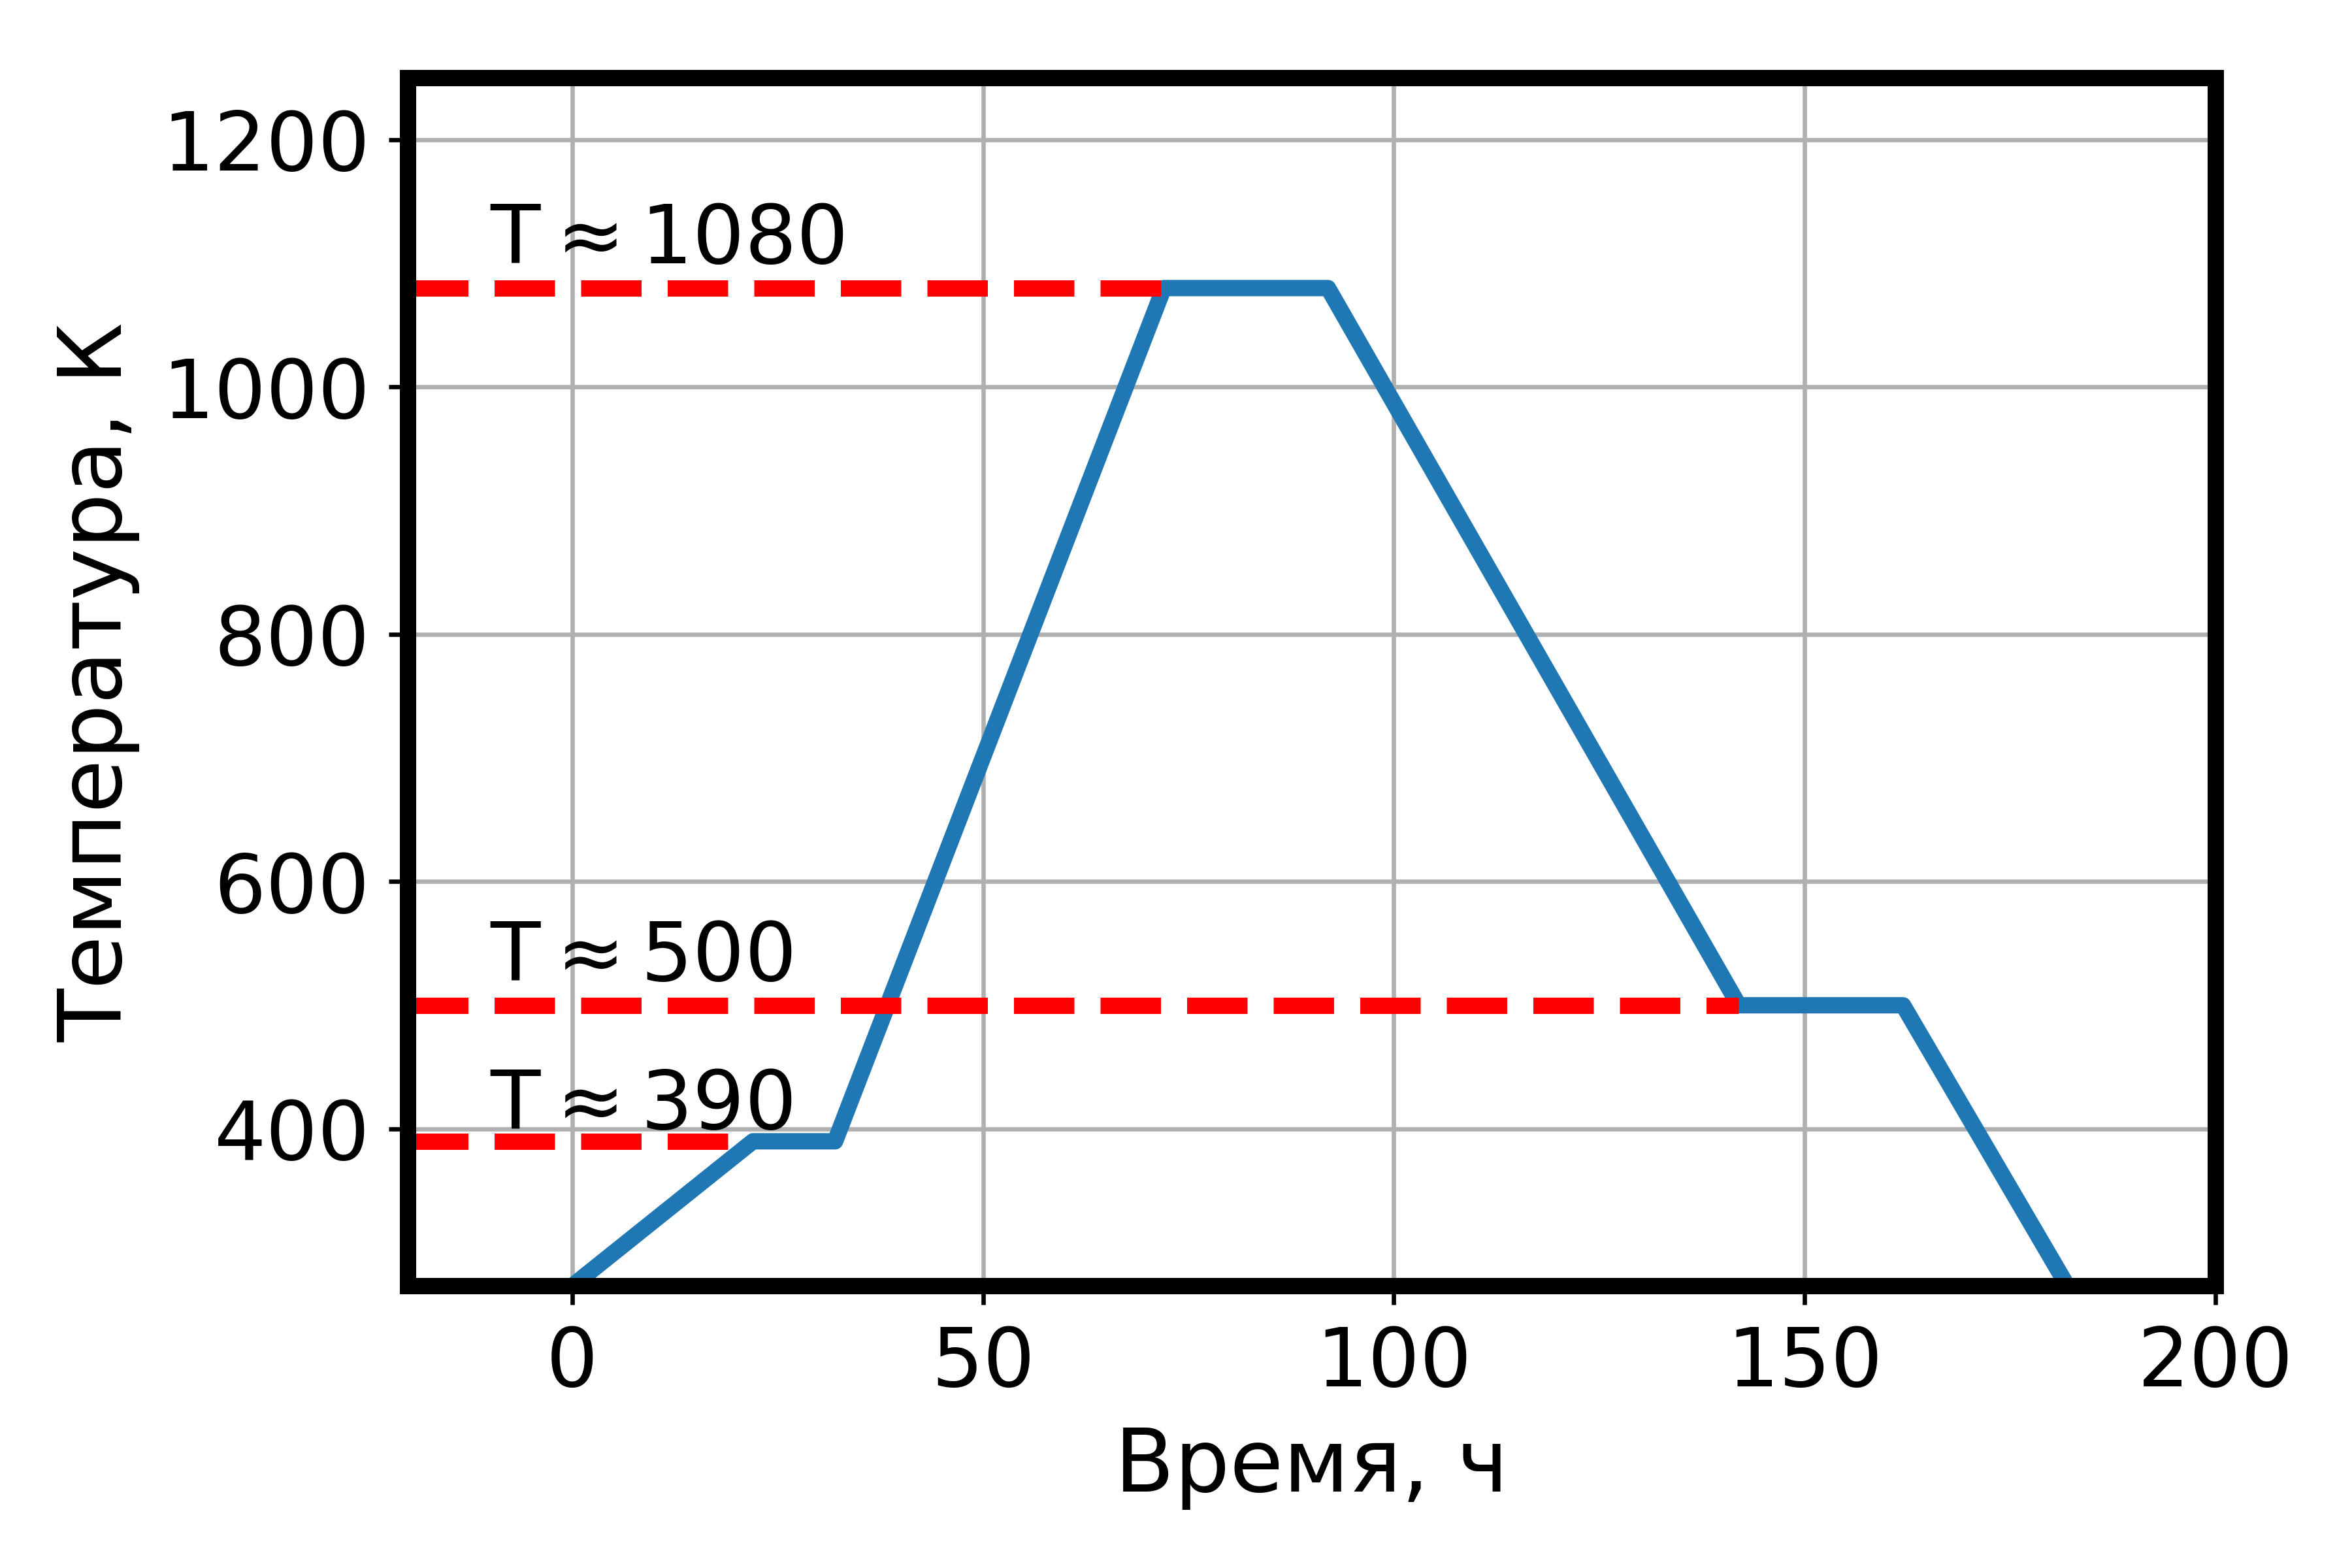
\includegraphics[width=0.99\linewidth]{5_synthesis}
  \end{minipage}
       \caption[Схема температурного режима синтеза соединений Cu\textsubscript{12}As\textsubscript{4}S\textsubscript{13} и Cu\textsubscript{12}Sb\textsubscript{4}S\textsubscript{13}]{Схема температурного режима синтеза соединений Cu\textsubscript{12}As\textsubscript{4}S\textsubscript{13} и Cu\textsubscript{12}Sb\textsubscript{4}S\textsubscript{13}(описание в тексте)}
    \label{img:figure3}
\end{figure}

Синтез соединений проводили в кварцевых ампулах при остаточном давлении 1$\cdot$10$^{-1}$~Па и заполненных обескислороженным аргоном или гелием при давлении 0.5$\cdot$10$^{5}$~Па. Очистку ампул проводили по схеме рекомендованной в \cite{156} с предварительной промывкой, травлением в азотной и фтористоводородной кислотах, промывкой дистиллированной водой и вакуумной сушкой в диапазоне температур от 900 до 1000~К и остаточном давлении 1$\cdot$10$^{-3}$~Па в течение 4--5~часов. Взвешивание исходных компонентов проводили на аналитических весах АВД--200 с точностью $\pm$5$\cdot$10$^{-5}$~г.
С целью компенсации ухода халькогена в газообразную фазу и обеспечения избыточного давления его паров в процессе синтеза навеску серы или селена делали с избытком (0.2--0.5\% по массе).
Для минерала cмитита показано\cite{181}, что избыточное содержание серы в таких количествах не выходит за пределы области гомогенности, но в то же время компенсирует уход халькогена в газообразную фазу и обеспечивает (вместе с давлением гелия или аргона) избыточное давление его паров в процессе синтеза, а также препятствует возникновению микропор в объеме синтезируемого соединения.
Точность определения температуры в~рабочей камере печи соответствовала 0,5~К при 600~К и 1~К при 1100~К (термопара платины и сплав платины с 10~\% родием использовалась для контроля температуры). Синтез проведен в~четыре этапа. Первый "--- медленное нагревание в~печи (10--15~часов) до~температуры, превышающей температуру плавления легколетучего компонента (серы или селена) на~10--30~К; второй "--- поддержание данной температуры 20--30~часов. Третий этап "--- увеличение температуры до~полного плавления образовавшегося в~ампуле вещества в течении 40--50~ч. и поддержание этой температуры постоянной 20--30 ч. Последний, четвертый этап  "--- понижение температуры до 2/3 от температуры плавления и отжиг соединения 30--40~ч.
 Пример схемы температурного режима представлен на рисунке \ref{img:figure3}. Образец Cu\textsubscript{12}As\textsubscript{4}S\textsubscript{13} после спекания дополнительно был подвергнут направленной перекристаллизации в~двухзонной печи по~методу Стокбаргера--Бриджмена. Часть образцов дополнительно была отожженна при~температуре 673 и 773~К в~течении 24~часов.
Перед отжигом образцы были перетерты в ступке и подвергнуты горячему прессованию.

\newpage
%============================================================================================================================
\section{Методы порошковой и монокристальной дифрактометрии} \label{sect2_2}
В этом разделе описаны методы прецизионных дифракционных экспериментов. Все полученные образцы аттестованы на порошковом дифрактометре D8
Advance (Bruker, Германия) на Cu K$\alpha$ излучении.
Характеристическое излучение данного дифрактометра монохроматизируется зеркалом Гёбеля, в нем используются щели Соллера  для формирования нужного геометрического размера пучка рентгеновского излучения. Порошкообразные образцы получены истиранием до гомогенного состояния. Рентгенофазовый анализ проведен методом порошка (Дебая--Шеррера) на образцах, которые  получены истиранием исходных спёченных образцов до гомогенного состояния в ступке. Дифрактограммы  обрабатывались в программном комплексе Jade 6 с использованием реферативной базы pdf2. Три соединения из синтезированных идентифицированы в кубической сингонии, одно --- в тетрагональной сингонии. Данные рентгенофазового анализа представлены в таблице \ref{xray_comp}.


\begin{table} [htbp]
\centering
\caption{Сводная таблица данных рентгенофазового анализа синтезированных соединений}%
	\label{xray_comp}% label всегда желательно идти после caption
    \renewcommand{\arraystretch}{1.5}
	\begin{tabular}{@{}@{\extracolsep{10pt}}llllllll@{}}
 \toprule     %%% верхняя линейка
     & &a,$\angstrom$  & b,$\angstrom$ & c,$\angstrom$  & $\alpha$,\textsuperscript{ $\circ$ }   & $\beta$,\textsuperscript{ $\circ$ } & $\gamma$,\textsuperscript{ $\circ$ }  \\ \midrule
Cu\textsubscript{12}As\textsubscript{4}S\textsubscript{13} & I$\overline{\! 4}$3m &\multicolumn{3}{c}{10.1439}  & \multicolumn{3}{c}{90}  \\ \hline
Cu\textsubscript{3}AsSe\textsubscript{3}                         & F$\overline{\! 4}$3m &\multicolumn{3}{c}{5.53}  & \multicolumn{3}{c}{90}     \\ \hline
Cu\textsubscript{12}Sb\textsubscript{4}S\textsubscript{13}  & I$\overline{\! 4}$3m &\multicolumn{3}{c}{10.30450}&\multicolumn{3}{c}{90}  \\ \hline
Cu\textsubscript{3}SbSe\textsubscript{3} & Pnma & 7.9865 & 10.6138 &6.837& \multicolumn{3}{c}{90} \\ \hline

 \bottomrule
\end{tabular}
\end{table}

Образец, полученный методом направленной перекристаллизации в~двухзонной печи по~методу Стокбаргера"--~Бриджмена, был подвергнут прецизионному дифракционному исследованию на монокристальном дифрактометре Xcalibur с 2d детектором CCD~EOS~S2 (Rigaku Oxford Diffraction). Образцы для измерений имели сферическую форму диаметром от 200 до 300~мкм, изготовленные специальным образом из скола от монокристаллического образца, или скола от пластинки образца толщиной 0.3~мм. Исследование проводилось при температурах 85, 115, 180, 250 и 293~К\cite{Dudka2016}. Температура определялась сенсором, который находился на сопле охлаждающей системы Cobra Plus. Хладагентом служил азот. Расстояние между соплом с хладагентом и образцом составляло 7~мм.

Детектор CCD~EOS~S2 и гониометр были предварительно откалиброваны экспериментально\cite{Dudka2010} с использованием монокристалла Ca\textsubscript{3}TaGa\textsubscript{3}Si\textsubscript{2}O\textsubscript{14}\cite{Dudka2016_b}. Полученная калибровка повысила точность получаемых данных на 10~\%.

Сбор данных, обработка и учет поглощения проводился в программном комплексе  CrysAlisPro. Коррекция поглощения на форму образца проведена интегральным методом Гаусса. Уточнение структуры произведено в программе Jana2000\cite{Dusek2001}.



%Используемая система основана на дифрактометре HUBER--5042, выпущенном в 1999 году, который был модифицирован в 2015--2017 годах. Модификация заключена в оснащении современным компьютером, поддерживающим новые скоростные протоколы передачи данных.
%Обмен данных между дифрактометром и персональным компьютером основан на блоке PCIDCC5--P, который выполняет роль устройства определяющего время и количество импульсов.
%Шаговые моторы дифрактометра управляются через интерфейс стандарта RS232. Вакуум внутри бриллиевых емкостей, где помещается образец, поддерживается турбомолекулярным насосом TPS-compact (Agilent Technologies). Охлаждающая система состоит из двух независимых устройств: охлаждение рентгеновской трубки и гелиового охлаждения образца.
%Программное обеспечение позволяет удалённо управлять измерительным комплексом.



Во время прецизионных  экспериментов использовалось MoK\textsubscript{$\alpha$}"~излучение ($\lambda$ = 0,71069~${\angstrom}$, графитовый монохроматор). Сбор данных проводился c использованием 2D детектора. Максимальное значение составляло $\theta$\textsubscript{max} = 42\textsuperscript{$\circ$}.
Угловые положения образца задавались с точностью 0.001\textsuperscript{$\circ$}.
Исходный R"~фактор усреднения R\textsubscript{уср}(I) составил не более чем 0.054, R/R\textsubscript{w} = 0.033/0.053 и уточнение проведено не менее чем по 11026 рефлексам.
Величины остаточных пиков разностной электронной плотности составили $\pm\Delta$$\rho$ = +2.7/$-$1.6.
Погрешность в параметрах ячейки не превышала 0.0002~{$\angstrom$}.

Дополнительно был проведен эксперимент на CAD4 с точечным детектором при комнатной температуре и на образце в форме сферы. Во время прецизионных экспериментов использовалось AgK\textsubscript{$\alpha$}"~излучение ($\lambda$ = 0,56083~${\angstrom}$, графитовый монохроматор). Сбор данных проводился при использовании точечного детектора по $\theta$/2$\theta$"~сканированию (c $\theta$\textsubscript{max} = 30\textsuperscript{$\circ$}).
Исходный R"~фактор усреднения R\textsubscript{уср}(I) составил не более чем  0.041, R/R\textsubscript{w} = 0.032/0.043 и уточнение проведено по 3509 рефлексам.
Величины остаточных пиков разностной электронной плотности составили $\pm\Delta$$\rho$ = +0.7/$-$0.9.
Погрешность в параметрах ячейки не превышала 0.0002~{$\angstrom$}.

\newpage
%============================================================================================================================
\section{Методы измерения и моделирования теплоёмкости} \label{sect2_4}
\subsection{Экспериментальное измерение теплоёмкости}\label{sect2_4_1}
Теплоёмкость синтезированных соединений измерена при помощи измерительного комплекса PPMS (Quantum Design,
США) в диапазоне температур от 2 до 350 К. Измерения проводились методом релаксации теплового
импульса\cite{Hwang_1997}. Измерительная установка представляет собой автономный комплекс с гелиевым криостатом замкнутого цикла. Данный метод основан на измерении времени релаксации теплового импульса. Преимущество метода заключается в том, что:
\begin{itemize}
\item Метод не критичен к размеру, форме образца и величине $\tau$\textsubscript{1}.

\item Метод позволяет измерять теплоёмкость в адиабатических и неадиабатических циклах в широком диапазоне температур.

\item Теплоёмкость автоматически определяется из прямых измерений  $\tau$\textsubscript{1} и $\tau$\textsubscript{2}.

\item Существует возможность ввести корректировки на учёт погрешности, вызванной нагреванием подложки, на которой находится образец.

\item Тепловое переключение не нужно.

\item Эффекты, связанные с $\tau$\textsubscript{2}, учитываются должным образом.
\end{itemize}


\begin{equation}
  \label{eq:equation2.2}
\begin{cases}
    P(t)=c'\frac{dT'}{dt}+\lambda_{s}(T'-T)+\lambda_{l}(T'-T_{0}) \\
    0 = c\frac{dT}{dt}+\lambda_{s}(T-T')
\end{cases} ,
\end{equation}

где c и T теплоёмкость и температура образца соответственно, с$'$ и T$'$ "--- теплоёмкость и температура держателя образца, P(t) "--- мощность, T\textsubscript{0} "--- температура теплоотвода, $\lambda$\textsubscript{l} "--- значение теплопроводности между теплоотводом и держателем образца, $\lambda$\textsubscript{s} "--- теплопроводность между образцом и держателем образца. Данное представление имеет место только в случае, если нагреватель и сенсор достаточно хорошо прикреплены к держателю образца и теплопроводность образца много больше, чем теплопроводности $\lambda$\textsubscript{l} и $\lambda$\textsubscript{s}.
Также допускается, что $\lambda$\textsubscript{l}, $\lambda$\textsubscript{s}, с и с$'$ температурно независимы от слабого изменения температуры.

Из системы уравнений \ref{eq:equation2.2} исключается T и учитывая, что P(t)~$=$~0 и dt$_{1}^{2}$/dt$^2$~$\cong$~0, получаем:

\begin{equation}
  \label{eq:equation2_4}
\cfrac{сc'}{\lambda_{s}}\cfrac{d^2T_1}{t^2}+\Bigg(c'+c+c\cfrac{\lambda_{l}}{\lambda_{s}}\Bigg)\cfrac{dT_1}{dt}+\lambda_{l}T_l=\lambda_{l}T_0.
\end{equation}


На основе математических преобразований в \cite{Hwang_1997} получаем выражение для теплоёмкости:

\begin{equation}
  \label{eq:equation2_3}
c'+c\cong c'+c\cfrac{\lambda_{l}}{\lambda_{s}}=\cfrac{P(t_{h})}{\frac{dT}{dt}\big|_{t=t_{h}}-\frac{dT}{dt}\big|_{t=t_{b}}}.
\end{equation}

Таким образом, измеряя значения времени регистрации, зная амплитуду теплового импульса и время нагрева, находим значение теплоёмкости исследуемого образца.

Экспериментальная схема измерения теплоёмкости на измерительном комплексе Quantum Design PPMS представлена на рисунке \ref{img:figure2}. Образец (4) помещается на платформу (5), которая висит в вакууме на тонких медных проводах (1). Эти тонкие медные провода служат теплоотводом (2) для теплоты, полученной от нагревателей (3 и 7). Образец крепится специальным гелем (6), обладающим постоянной теплоёмкостью в широком диапазоне температур.
\begin{figure}[ht]
  \begin{minipage}[ht]{0.99\linewidth}\centering
    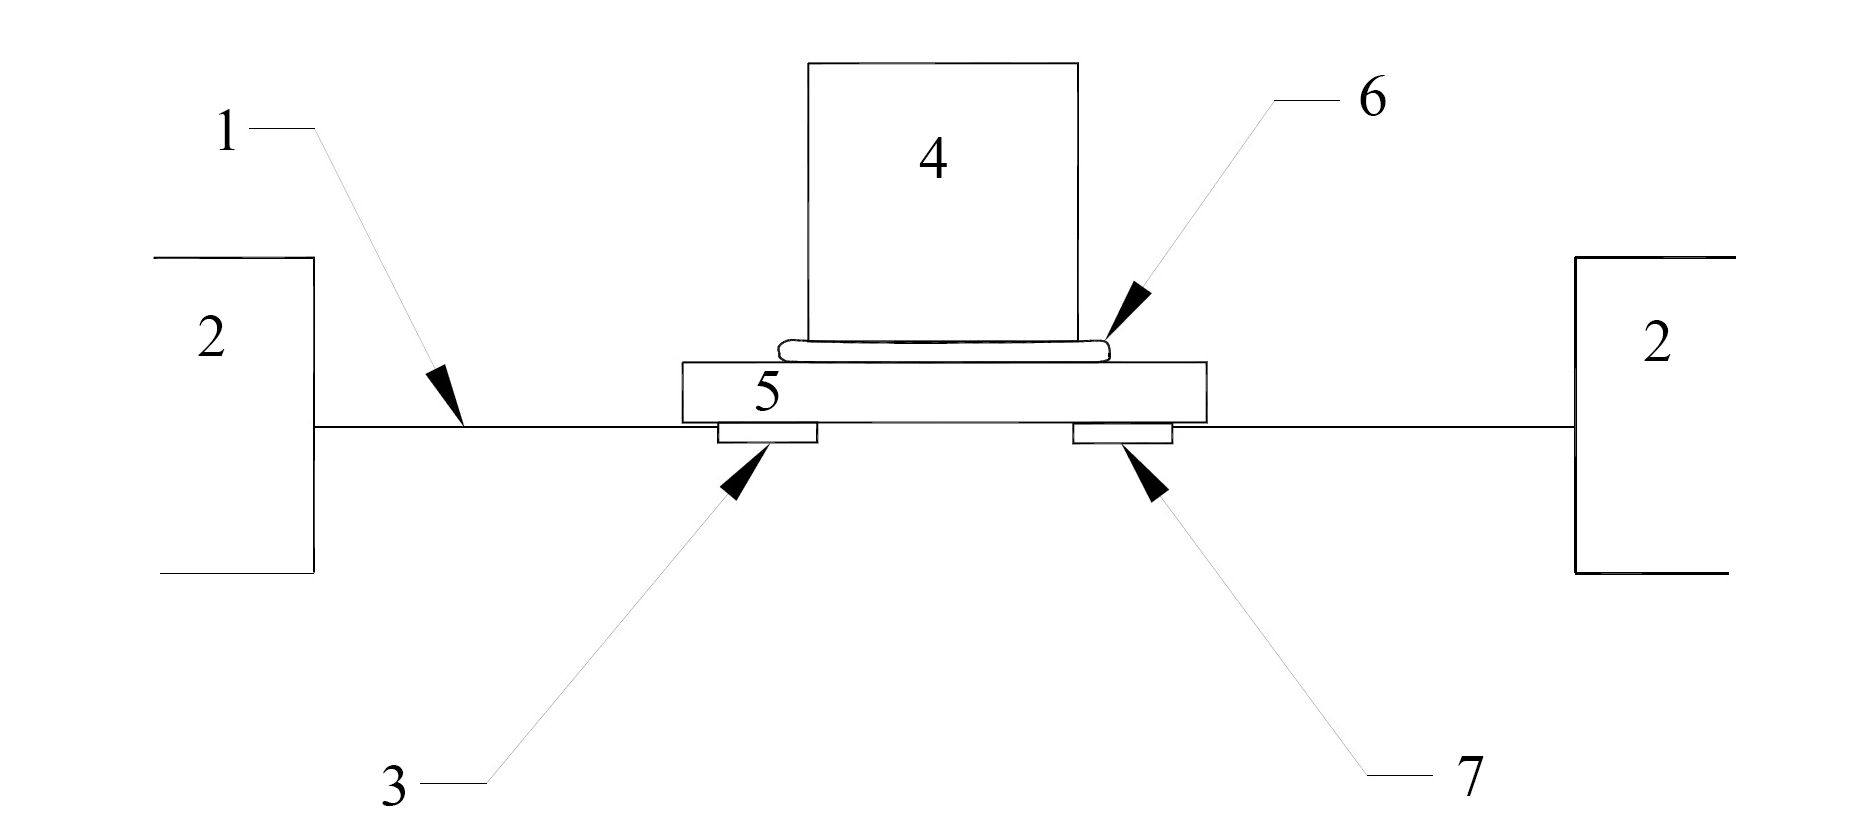
\includegraphics[width=0.99\linewidth]{4_heat_capacity_scheme}
  \end{minipage}
       \caption[Схематическое изображение схемы измерения теплоёмкости на измерительном комплексе Quantum Design PPMS]{Схематическое изображение схемы измерения теплоёмкости на измерительном комплексе Quantum Design PPMS. 1 "--- медные провода, 2 "--- теплоотвод, 3 и 7 "--- нагреватель, 4 "--- образец, 5 "--- платформа образца, 6 "--- теплопроводящий гель (описание дано в тексте)}
    \label{img:figure2}
\end{figure}

\begin{figure}[p!]
  \begin{minipage}[ht]{0.99\linewidth}\centering
    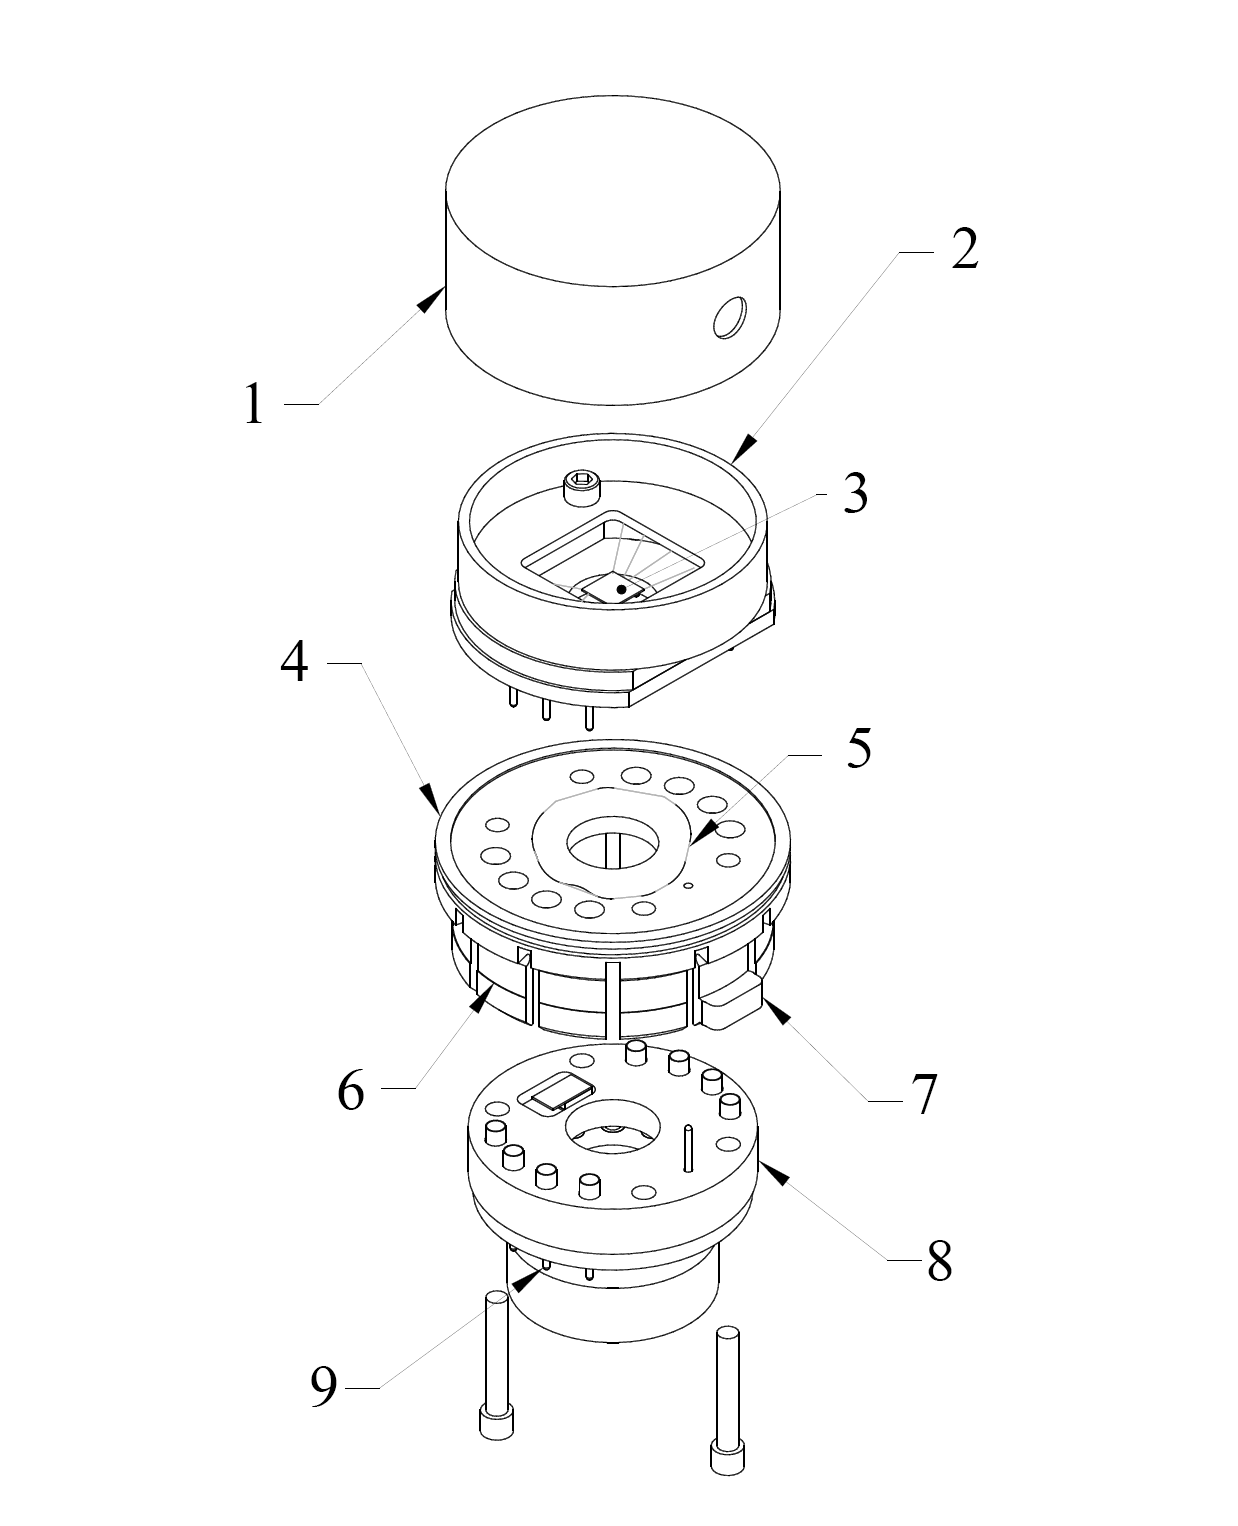
\includegraphics[width=0.99\linewidth]{5_heat_capacity_cell}
  \end{minipage}
       \caption[Схематическое изображение ячейки для измерения теплоёмкости на измерительном комплексе Quantum Design PPMS]{Схематическое изображение ячейки для измерения теплоёмкости на измерительном комплексе Quantum Design PPMS. 1 "--- защитный колпак, 2 "--- основание ячейки, 3 "--- место крепления образца, 4 "--- зажимной патрон, 5 "--- теплопроводящий гель, 6 "--- зажимы, 7 "--- индикатор положения основания ячейки, 8 "--- интерфейс, 9 "--- выходные контакты (описание дано в тексте)}
    \label{img:figure3}
\end{figure}


Описанная выше схема измерения теплоёмкости (рис. \ref{img:figure2}) реализуется в специальной ячейке, которая схематически изображена на рисунке \ref{img:figure3}. Используемая ячейка представляет собой капсулу, которая закрывается медной крышкой (1). Данная крышка выполняет  роль дополнительного теплоотвода. Крышка (1) крепится на основание (2), которое выполняет защитную функцию. На данном основании находится платформа для образца, показанная на \ref{img:figure2}. Основание (2) крепится в зажимной патрон (4), на который нанесен теплопроводящий гель (5). Зажимной патрон и основание с образцом надеваются на интерфейс (8) с помощью зажимов (6). Правильное положение крепления определяется индикатором (7). Через контакты (9) выводятся регистрируемые значения.

\subsection{Моделирование теплоёмкости}\label{sect2_4_2}
Расчётная кривая теплоёмкости получена вычислением функции Дебая с тремя дополнительными осцилляторами Эйнштейна. В теории Дебая предполагается, что атомы в кристаллической решетке являются материальными точками, которые колеблются как гармонические осцилляторы.
Каждый из этих атомов обладает 3N колебательными модами и подчиняется распределению Планка.
Теорией Дебая также предполагалось, что существует зависимость частот упругих колебаний от волнового вектора $\omega$~$=$~$\omega$(K), частота колебаний ограничивается максимальной частотой $\omega$\textsubscript{max}. При описании осцилляторов Эйнштейна подразумевается, что описываемые фононные моды квантуются, и что энергия нулевых колебаний не зависит от температуры.

Расчётная кривая теплоёмкости получена вычислением функции Дебая с тремя дополнительными осцилляторами Эйнштейна. Добавление осцилляторов Эйнштейна обсуждается в описании экспериментальных данных и обуславливает наличие мягких фононных мод в соединениях. Общая формула, по которой проводилось вычисление, имеет вид:

\begin{equation}
  \label{eq:equation2_4}
C_p(T)=9R\cfrac{T^3}{\theta_d^3}\int\limits_0^{\frac{\theta_d}{T}}\frac{e^xx^4}{(e^x-1)^2}dx+3R\sum_{i=1}^3\cfrac{e^{\frac{\theta_{e_i}}{T}}\big(\frac{\theta_{e_i}}{T}\big)^2}{\big(\frac{\theta_{e_i}}{T}-1\big)^2},
\end{equation}

где $\theta$\textsubscript{d} "--- температура Дебая, $\theta$\textsubscript{$e_i$} "--- температура соответствующего осциллятора Эйнштейна.
Осцилляторы Эйнштейна описывают дополнительный вклад в общий фононный спектр в кристаллической решетке.
Для каждого соединения дополнительные осцилляторы Эйнштейна подбирались индивидуально на основании  литературных данных и полученнх экспериментальных результатов.
\newpage
%============================================================================================================================
\section{Просвечивающая электронная микроскопия} \label{sect2_4}

Изображения структуры получены на электронном микроскопе FEI Titan 80--300 в режиме HAADF-STEM  при ускоряющем напряжении 300 кВ.
HAADF режим дает контраст по атомному номеру (зависимость Z\textsuperscript{2}).
Образец приготовлен с помощью системы фокусированного ионного пучка (FIB) на двухлучевом сканирующем микроскопе "--- FEI Helios 600.
Изображения получены при комнатной температуре на ламельке толщиной менее 100~нм в (011) плоскости синтетического теннантита  Cu\textsubscript{12}As\textsubscript{4}S\textsubscript{13}.


Обработка изображений произведена в программном обеспечении atomap\cite{Nord2017}. С помощью программного обеспечения было проведено определение колонок атомов и их эллиптичность. Использовалась версия программы, которая оптимизирована для обработки кубических структур. Дополнительно был учтен дрейф и получены изображения \ref{img:mic}, показывающие величину эллиптичности для рядов атомов в (011) плоскости.

Изображения обработаны по следующему алгоритму:
\begin{itemize}
\item Нахождение колонок на изображении.

\item Вычитание найденных рядов, повторный поиск, введение нескольких решеток с одинокой интенсивностью.

\item Нахождение центров пиков изображения.

\item Анализ формы интенсивности от колонок, нахождение эллиптичности.

\item Учет дрейфа.
\end{itemize}

На рисунке \ref{img:mic1}а) "--- оригинальное изображение, полученное на микроскопе. На рисунке \ref{img:mic1}б) представлено обработанное изображение, на котором отмечены найденные ряды. А на рисунках \ref{img:mic1}в) и \ref{img:mic1}г) изображены значение эллиптичности для  мышьякового и медного рядов (011) плоскости соответственно.
Программно это определяется с помощью подбора оптимальных параметров для системы уравнений:
\begin{figure}[p!]
  \begin{minipage}[ht]{0.5\linewidth}\centering
    
\includegraphics[width=0.7\linewidth]{mic_Figure_10} \\ а)
  \end{minipage}
  \hfill
  \begin{minipage}[ht]{0.5\linewidth}\centering
    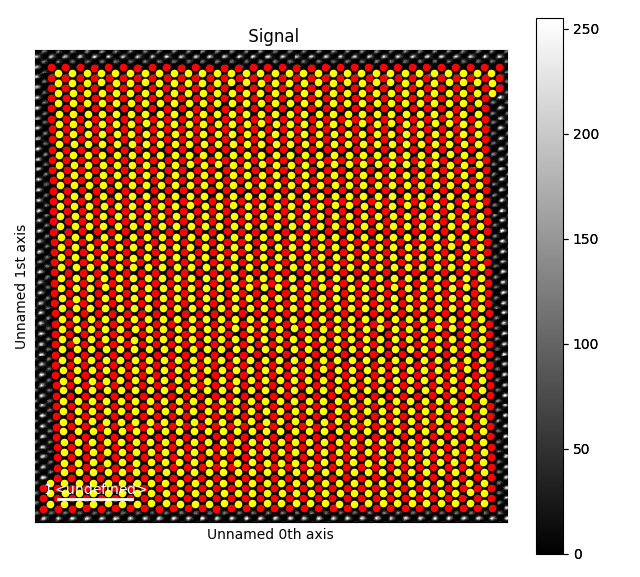
\includegraphics[width=0.9\linewidth]{mic_Figure_10_example} \\ б)
  \end{minipage}
\vfill
  \begin{minipage}[ht]{0.5\linewidth}\centering
    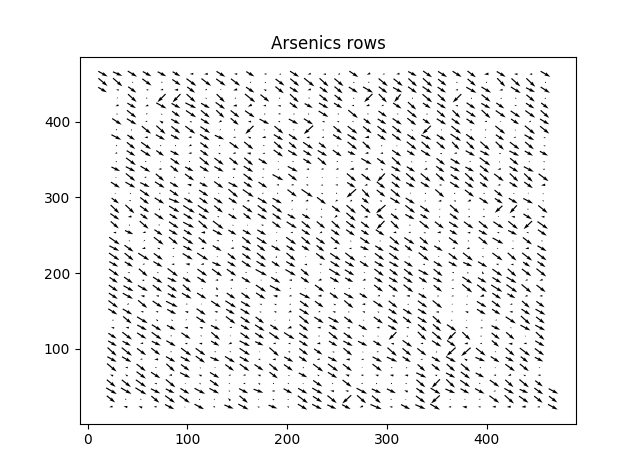
\includegraphics[width=0.9\linewidth]{mic_Figure_10_arsenic_raw} \\ в)
  \end{minipage}
  \hfill
  \begin{minipage}[ht]{0.5\linewidth}\centering
    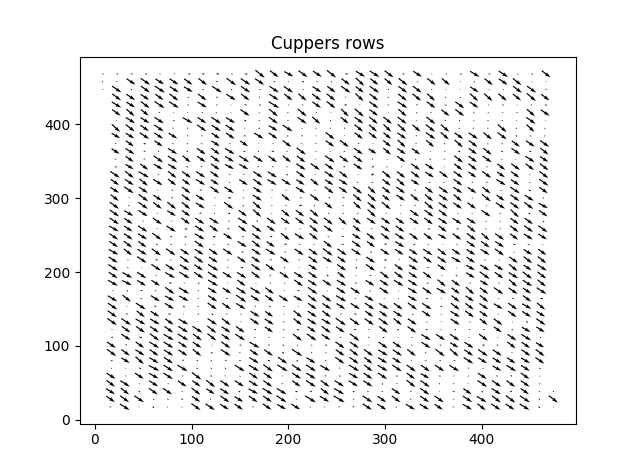
\includegraphics[width=0.9\linewidth]{mic_Figure_10_cupper_raw} \\ г)
  \end{minipage}

      \caption[Изображения структуры в режиме HAADF-STEM (а, б) и эллиптичность рядов мышьяка (в) и меди (г) синтетического теннантита Cu\textsubscript{12}As\textsubscript{4}S\textsubscript{13} в (011) плоскости]{Изображения структуры в режиме HAADF-STEM (а, б) и эллиптичность рядов мышьяка (в) и меди (г) синтетического теннантита Cu\textsubscript{12}As\textsubscript{4}S\textsubscript{13} в  (011) плоскости}
    \label{img:mic1}
\end{figure}

\begin{equation}
  \label{eq:equation_mic}
	\begin{cases}
	I(x,y) = I_0+Aexp(-(a(x-x_0)^2-\\
	\qquad-2b(x-x_0)(y-y_0)+c(y-y_0)^2)) \\
	a=\cfrac{\cos^2\theta}{2\sigma^2_x}+\cfrac{\sin^2\theta}{2\sigma^2_y} \\
	b= - \cfrac{\sin2\theta}{4\sigma^2_x}+\cfrac{\sin2\theta}{4\sigma^2_y}\\
	c= \cfrac{\sin^2\theta}{2\sigma^2_x}+\cfrac{\cos^2\theta}{2\sigma^2_y} \\
	\end{cases},
\end{equation}
где I\textsubscript{0} "--- интенсивность фона, A "--- амплитуда центра пика, x\textsubscript{0} и y\textsubscript{0} "--- координаты центра ряда, $\sigma_x$ и $\sigma_y$ "--- стандартное отклонение, $\theta$ "--- угол поворота эллиптичности столбца.

Эллиптичность определяется по соотношению:
\begin{equation}
  \label{eq:equation_mic2}
\epsilon =
	\begin{cases}
	\cfrac{\sigma_x}{\sigma_y}, если \sigma_x > \sigma_y \\
	\cfrac{\sigma_y}{\sigma_x}, если \sigma_y > \sigma_x
	\end{cases}.
\end{equation}
\newpage
%============================================================================================================================
\section{Квантовомеханические рассчёты} \label{sect2_5}
Квантовомеханические вычисления проводились в рамках теории функционала плотности. Теория функционала плотности основывается на представлении, что электронная структура определяется распределением электронной плотности.
Вычисления проводились с использованием программы VASP (Vienna Ab initio Simulation Package) \cite{Kresse1993,Kresse1994,Kresse1996}.
Эта программа позволяет проводить квантовохимические расчёты из первых принципов (ab initio) на основе функционалов метода локальной электронной плотности и обобщённого градиента в параметризации Пердью"--~Бурке"--~Эрнзерхофа (Perdew"--~Burke"--~Ernzerhof)\cite{Perdew1996}.
Вычисления основаны на методе присоединённых плоских волн, равновесная атомная геометрия зоны Бриллюэна была разбита с помощью метода Монкхоста"--~Пака (Monkhorst"--~Pack) \cite{Monkhorst_1976} на 6$\times$6$\times$6~точек. Величина энергии обрезания в расчёте равнялась 450~эВ. Оптимизация атомной структуры проводилась до тех пор, пока межатомные силы не становились меньше 0.001~эВ/${\angstrom}$.



\newpage
%============================================================================================================================
\section{Измерения намагниченности} \label{sect2_6}
Магнитные свойства образцов измерены с
помощью магнитоизмерительного комплекса
MPMS"--~XL7~EC (Quantum Design, США) с первичным преобразователем на основе СКВИДа (от англ. SQUID, Superconducting Quantum Interference Device "--- сверхпроводящий квантовый интерферометр) в диапазоне температур от 2 до 350 К и в постоянных магнитных полях напряженностью до 70 кЭ. Шаг измерения в диапазоне от $-$5 до 5~кЭ составлял 0.1~Э, при больших полях "--- 1~Э. В измерительном приборе существует возможность перевода сверхпроводящего соленоида в нормальное состояние для стабилизации поля.
Магнитоизмерительный комплекс MPMS--XL7~EC может регистрировать значения магнитного момента до 1$\cdot$10\textsuperscript{-8}~Гс$\cdot$см\textsuperscript{3}.
В базовой комплектации измерительный комплекс позволяет проводить магнитометрические измерения в диапазоне от 1.8 до 400~К.
Абсолютная погрешность измерения температуры составляет не более $\pm$0.5~\% в указанном выше диапазоне температур.
Погрешность измерений магнитного момента для нанокристаллических образцов и образов с постоянными магнитными моментами $\delta$\textsubscript{P~$=$~0.95}~$=$~$\pm$1.0~\%.
Для проведения измерений намагниченности образец крепили на длинную
ленту каптона внутри пластиковой трубочки, размеры которой существенно больше линейных размеров образца и градиентометра второго порядка,
состоящего из четырех измерительных витков.
Вклад от элементов крепления был полностью исключен в процессе измерения. Источником постоянного магнитного поля являлся сверхпроводящий
соленоид на основе соединения Nb\textsubscript{3}Sn.


Магнитная восприимчивость $\chi$ имеет две основные составляющие: диамагнитную, характеризующуюся магнитным моментом, возникающим на заполненных электронных оболочках, и парамагнитную, обусловленную наличием неспаренных электронов. Согласно теории Кюри"--~Вейсса магнитная
восприимчивость может быть описана выражением:

\begin{equation}
  \label{eq:equation2.1}
  \chi = \chi_{dia}+\frac{C}{T - \Theta}.
\end{equation}

Диамагнитная составляющая магнитной восприимчивости $\chi_{dia}$ найдена из графика функции
магнитной восприимчивости от обратной температуры, а температура $\Theta$ "--- из графика функции обратной магнитной восприимчивости от
температуры путём экстраполяции экспериментальной кривой.

\newpage
%============================================================================================================================
\section{Измерение спектров комбинационного рассеяния} \label{sect2_6}

Спектры комбинационного рассеяния получены на спектрометре TRIAX-552, оборудованном охлаждаемым детектором Peltier TE CCD SPEC 10 (Princeton Instruments).
Были использованы: решетка 600 штрихов на мм и 50-кратная линза Mitutoyo M Plan Apo SL50 (числовая апертура 0.42).
Для получения возбуждающей линии использован аргон-ионный лазер с длинной волны 514.5 нм Spectra-Physics Stabilite 2017 и с выходной мощностью от 0.3 до 1~мВт на образце. Калибровка проведена с использованием линии спектра комбинационного рассеяния света 520.5~см\textsuperscript{-1} полированной кремниевой пластины и/или линий спектра комбинационного рассеяния неона.
Для наблюдения спектра комбинационного рассеяния света вблизи возбуждающей линии использовались 3  брэгговских фильтра.

На схеме (Рис. \ref{img:raman}) для получения спектров комбинационного света представлено расположение используемого оборудования. Инструментальная погрешность составила 4~см\textsuperscript{-1}.
\begin{figure}[p!]
  \begin{minipage}[ht]{0.99\linewidth}\centering
    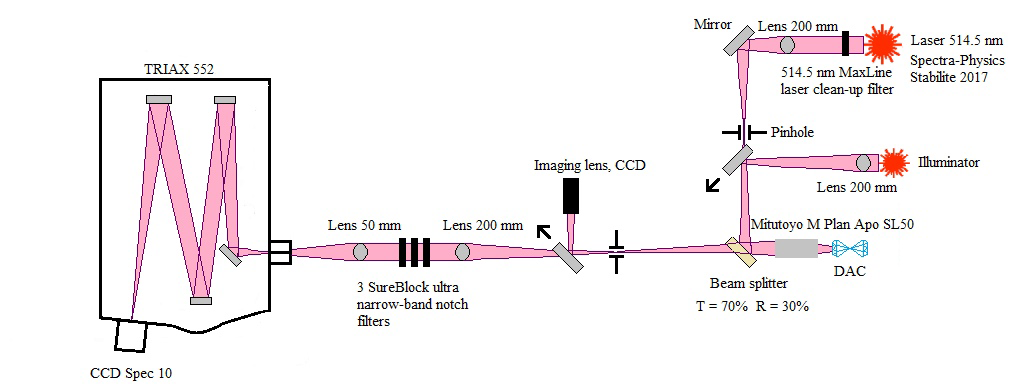
\includegraphics[width=0.99\linewidth]{raman_scheme}
  \end{minipage}


      \caption[Схематическое изображение спектрометра комбинационного рассеяния]{Схематическое изображение спектрометра комбинационного рассеяния}
    \label{img:raman}
\end{figure}
\newpage

\section{Выводы по Главе 2} \label{sect2_7}

В главе описаны основные методы и методики исследования и синтеза соединений для систем Cu--As--S, Cu--Sb--S, Cu--As--Se и Cu--Sb--Se в стехиометрическом соотношении 3:1:3.
А именно: методы порошковой и монокристальной дифрактометрии, измерения и моделирования теплоёмкости, просвечивающей электронной микроскопии и измерения магнитной восприимчивости.

Соединения Cu\textsubscript{12}V\textsubscript{4}VI\textsubscript{13}, где V = As, Sb и VI = S, Se синтезированы в~кварцевых ампулах с инертной средой. В~качестве исходных материалов использованы реактивы высокой чистоты не ниже марки <<особо чистый>>.
Рентгенофазовый анализ осуществлен методом порошка, дифрактограммы  обрабатывались в~программном комплексе Jade~6 с использованием реферативной базы pdf2.
Прецизионное исследование структуры монокристалла теннантита проведено на четырехкружном автоматическом дифрактометре Xcalibur c 2d детектором  CCD~EOS~S2 и с~системой охлаждения Cobra Plus при температурах 85, 115, 180, 250 и 293~K.
Изображения атомных структур получены на электронном микроскопе FEI Titan 80--300 в режиме HAADF-STEM  при ускоряющем напряжении 300 кВ.
Образец приготовлен с помощью системы фокусированного ионного пучка (FIB) на двухлучевом сканирующем микроскопе "--- FEI Helios 600.
Теплоёмкость измерена при помощи измерительного комплекса PPMS (Quantum Design, США) в диапазоне температур от 2 до 350 К. Измерения проводились методом релаксации теплового импульса\cite{Hwang_1997}.
Квантовомеханические вычисления проводились в рамках теории функционала плотности с использованием программы VASP (Vienna Ab initio Simulation Package) \cite{Kresse1993,Kresse1994,Kresse1996}, основанной на методе присоединённых плоских волн.
Спектры комбинационного рассеяния получены на спектрометре TRIAX-552, оборудованном охлаждаемым детектором Peltier TE CCD SPEC 10 (Princeton Instruments).
Магнитные свойства образцов измерены с помощью магнитоизмерительного комплекса MPMS--XL7~EC (Quantum Design, США) с первичным преобразователем на основе СКВИДа в~диапазоне температур от 2 до 350 К и в постоянных магнитных полях напряженностью до 70 кЭ.

\newpage
           % Глава 2
 \chapter{Особенности формирования лавесовского полиэдра на примере синтетического теннантита Cu\textsubscript{12}As\textsubscript{4}S\textsubscript{13}} \label{chapt3}

В данной главе описаны результаты исследования монокристаллического образца синтетического теннантита Cu\textsubscript{12}As\textsubscript{4}S\textsubscript{13} методами монокристальной дифрактометрии в диапазоне температур от 85 до 293~К, просвечивающей микроскопии монокристаллического образца в плоскости (011) и моделирования структур теннантита с разным расположением атомов в лавесовском полиэдре методом первопринципных расчётов.



\section{Рентгеноструктурный анализ синтетического теннантита Cu\textsubscript{12}As\textsubscript{4}S\textsubscript{13} в диапазоне температур от 85 до 293~К} \label{sect3_1}

Исследование монокристаллического образца  Cu\textsubscript{12}As\textsubscript{4}S\textsubscript{13} проведено при температурах 85, 115, 180, 250 и 293~К. Образец обладал сложной формой с линейными размерами от 100 до 300~мкм и являлся сколом от монокристалла.  Результаты дифракционных экспериментов при разных температурах представлены в таблице~\ref{xray1}. С понижением температуры объём элементарной ячейки ожидаемо уменьшается и возрастает значение R-фактора.
Также с~понижением температуры возрастает заселенность позиции Cu2 (pис.~\ref{img:xray}a) и  наблюдается аномальное изменение значения коэффициента атомарного смещения для позиции S2 (pис.~\ref{img:xray}б), которое показывает наличие фазового перехода второго рода в диапазоне от 115 до 180 К.

\begin{landscape}
\begin{table} [htbp]
\centering
\caption{Сводная таблица данных рентгеноструктурных исследований для синтетического теннантита Cu\textsubscript{12}As\textsubscript{4}S\textsubscript{13} при температурах 85, 115, 180, 250 и 293~К}%
	\label{xray1}% label всегда желательно идти после caption
    \renewcommand{\arraystretch}{1.5}
	\begin{tabular}{@{}@{\extracolsep{20pt}}llllll@{}}
 \toprule     %%% верхняя линейка
T, K                       & 85          & 115         & 180         & 250         & 293         \\
   \midrule
a, $\angstrom$                       & 10.1439(2)  & 10.1446(2)  & 10.1463(2)  & 10.1523(2)  & 10.1572(2)  \\ \hline
V, $\angstrom^3$                      & 1043.79(4)      & 1044.01(4)      & 1044.54(4)      & 1046.39(4)      & 1047.91(4)      \\ \hline
Группа симметрии                     &\multicolumn{5}{c}{ I–43m  }                                         \\ \hline
Длина волны, ($\angstrom$) & \multicolumn{5}{c}{Mo K\textsubscript{$\alpha$}, 0.71069 } \\ \hline
Дифрактометр             & \multicolumn{5}{c}{Xcalibur}                                       \\ \hline
Коррекция абсорбции      & \multicolumn{5}{c}{аналитическая (по форме кристалла)} \\ \hline
$\theta_{max}$,\textsuperscript{ $\circ$ }                 &  \multicolumn{5}{c}{42.08 } \\ \hline
R\textsubscript{int}                       & 0.052       & 0.054       & 0.049       & 0.050       & 0.049       \\ \hline
N\textsubscript{ref} , регистрированный           & 11028       & 11029       & 11036       & 11010       & 11026       \\ \hline
I $\geq \sigma$(I)                  & 693         & 691         & 686         & 677         & 667         \\ \hline
N\textsubscript{paf}                       & 36          & 42          & 47          & 47          & 44          \\ \hline
GOF                        & 1.06        & 1.15        & 1.03        & 1.01        & 1.00        \\ \hline
R/R\textsubscript{w}                     & 0.034/0.052 & 0.037/0.056 & 0.031/0.045 & 0.032/0.045 & 0.029/0.038 \\ \hline
$\pm\Delta\rho   $                     & +2.9/–1.8   & +3.5/–1.7   & +2.3/–1.1   & +1.8/–1.1   & +1.7/–1.2   \\ \hline
R\textsubscript{MEM}                     & 0.017/0.021 & 0.016/0.021 & 0.018/0.022 & 0.018/0.022 & 0.019/0.021\\ \hline
 \bottomrule
\end{tabular}
\end{table}
\end{landscape}


\begin{landscape}
\begin{table} [htbp]
\centering
\caption{Сводная таблица положения некоторых атомов и величины параметров их атомного смещения для синтетического теннантита Cu\textsubscript{12}As\textsubscript{4}S\textsubscript{13} при температурах 85, 115, 180, 250 и 293~К}%
	\label{xray2}% label всегда желательно идти после caption
    \renewcommand{\arraystretch}{1.5}
	\begin{tabular}{@{}@{\extracolsep{20pt}}llllll@{}}
 \toprule     %%% верхняя линейка
T, K             	          & 85 	         & 115  	       & 180    	     & 250    	     & 293         \\
   \midrule
Заселенность, Cu(2) & 0.758(3)    & 0.752(3)    	 & 0.703(10)     & 0.686(11)    & 0.679(11)    \\
x, Cu(2)         		 & 0.2173(3)   & 0.2176(3)   	 & 0.2177(4)   	& 0.2176(4)   & 0.2172(5) \\
x, Cu(21)        		 & 0.2123(4)   & 0.2124(4)   	 & 0.2130(10)   & 0.2137(12)   & 0.2149(12)   \\
y, Cu(21)       		 & 0.0777(3)   & 0.0776(4)   	 & 0.0694(19)   & 0.0675(19)   & 0.0662(19)   \\
x, As(1)         		& 0.24271(11)  & 0.24265(12)  	 & 0.24177(10)  & 0.24169(10)  & 0.24162(4)  \\
x. S(1)          		& 0.35734(10) & 0.3575(2) 	 & 0.35734(8)  & 0.35730(8)  & 0.35722(7)  \\
–y, S(1)         		 & 0.11822(7) & 0.11807(14)	 & 0.11850(6) 	& 0.11853(6) & 0.11854(6) \\
U\textsubscript{eq},$ \times$10\textsuperscript{4}, Cu(1)   & 69.8(12)       & 83.1(14)       & 111(3)      	    & 155(3)       & 184(3)      \\
U\textsubscript{eq},$ \times$10\textsuperscript{4}, Cu(2)   & 196(2)   	& 216(3)          & 234(3)         & 295(4)       & 339(5)      \\
U\textsubscript{eq},$ \times$10\textsuperscript{4}, Cu(21)  & 134(8)      	& 174(9)          & 320(30)       & 390(30)     & 420(30)     \\
U\textsubscript{eq},$ \times$10\textsuperscript{4}, As(1)   & 76.4(10)     	& 84.6(10)      & 88.3(8)         & 103.8(8)    & 114.0(7)    \\
U\textsubscript{eq},$ \times$10\textsuperscript{4}, S(1)    & 76.4(15)    	& 80.8(16)      & 79.5(13)        & 97.2(13)    & 111.0(13)   \\
U\textsubscript{eq},$ \times$10\textsuperscript{4}, S(2)    & 175(9)      	& 167(9)         & 133(7)  	     & 139(7)       & 160.7(7)  \\ \hline
 \bottomrule
\end{tabular}
\end{table}
\end{landscape}

Температурное исследование показывает изменение  заселенности в позиции меди Cu21 при понижении температуры (см. \ref{img:structure1}). На рисунке \ref{img:structure2} показано изменение  параметров атомного смещения и расстояния между позициями Cu21--S2.
На Рис. \ref{img:figure2} представлена электронная плотность для расстояния 2 $\angstrom$ от центра ячейки для синтетического теннантита Cu\textsubscript{12}As\textsubscript{4}S\textsubscript{13} (данные получены впервые) и синтетического тетраэдрита Cu\textsubscript{12}Sb\textsubscript{4}S\textsubscript{13} (литературные данные), по которым видно неоднозначное распределение для атомов меди.

\begin{figure}[p!]
  \begin{minipage}[ht]{0.9\linewidth}\centering
    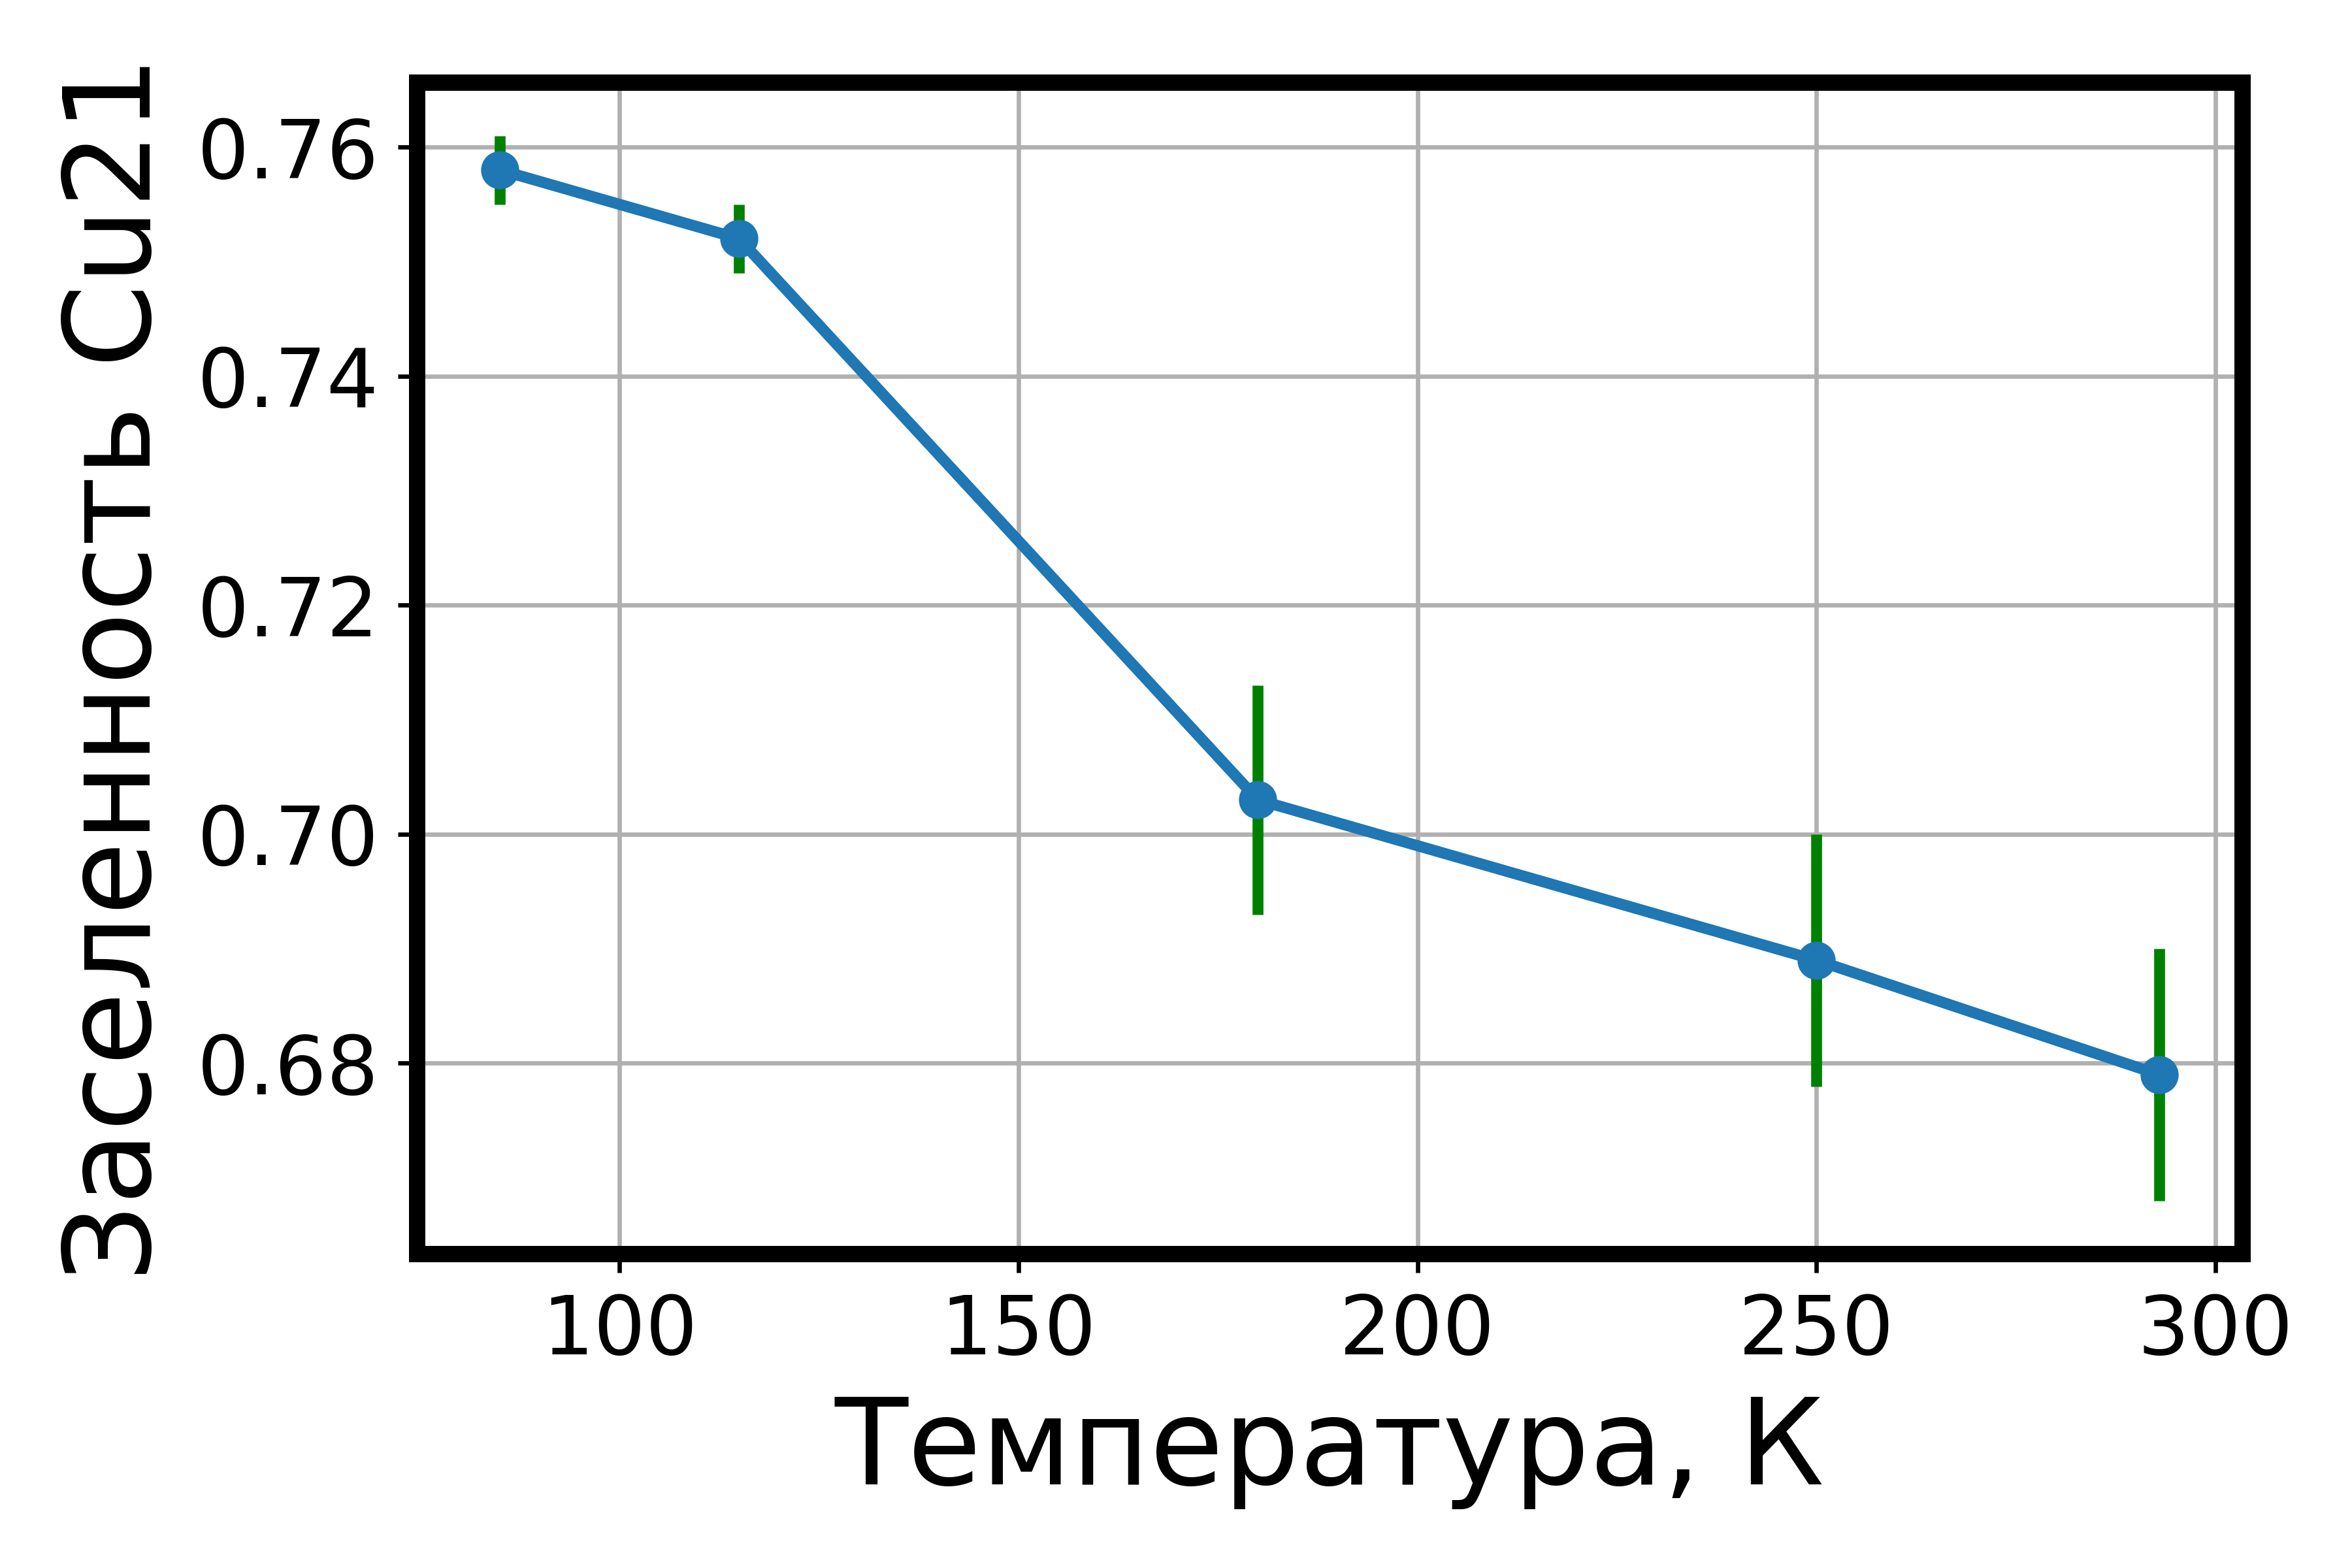
\includegraphics[width=0.9\linewidth]{structure_occCu2} \\ а)
  \end{minipage}
  \vfill
  \begin{minipage}[ht]{0.9\linewidth}\centering
    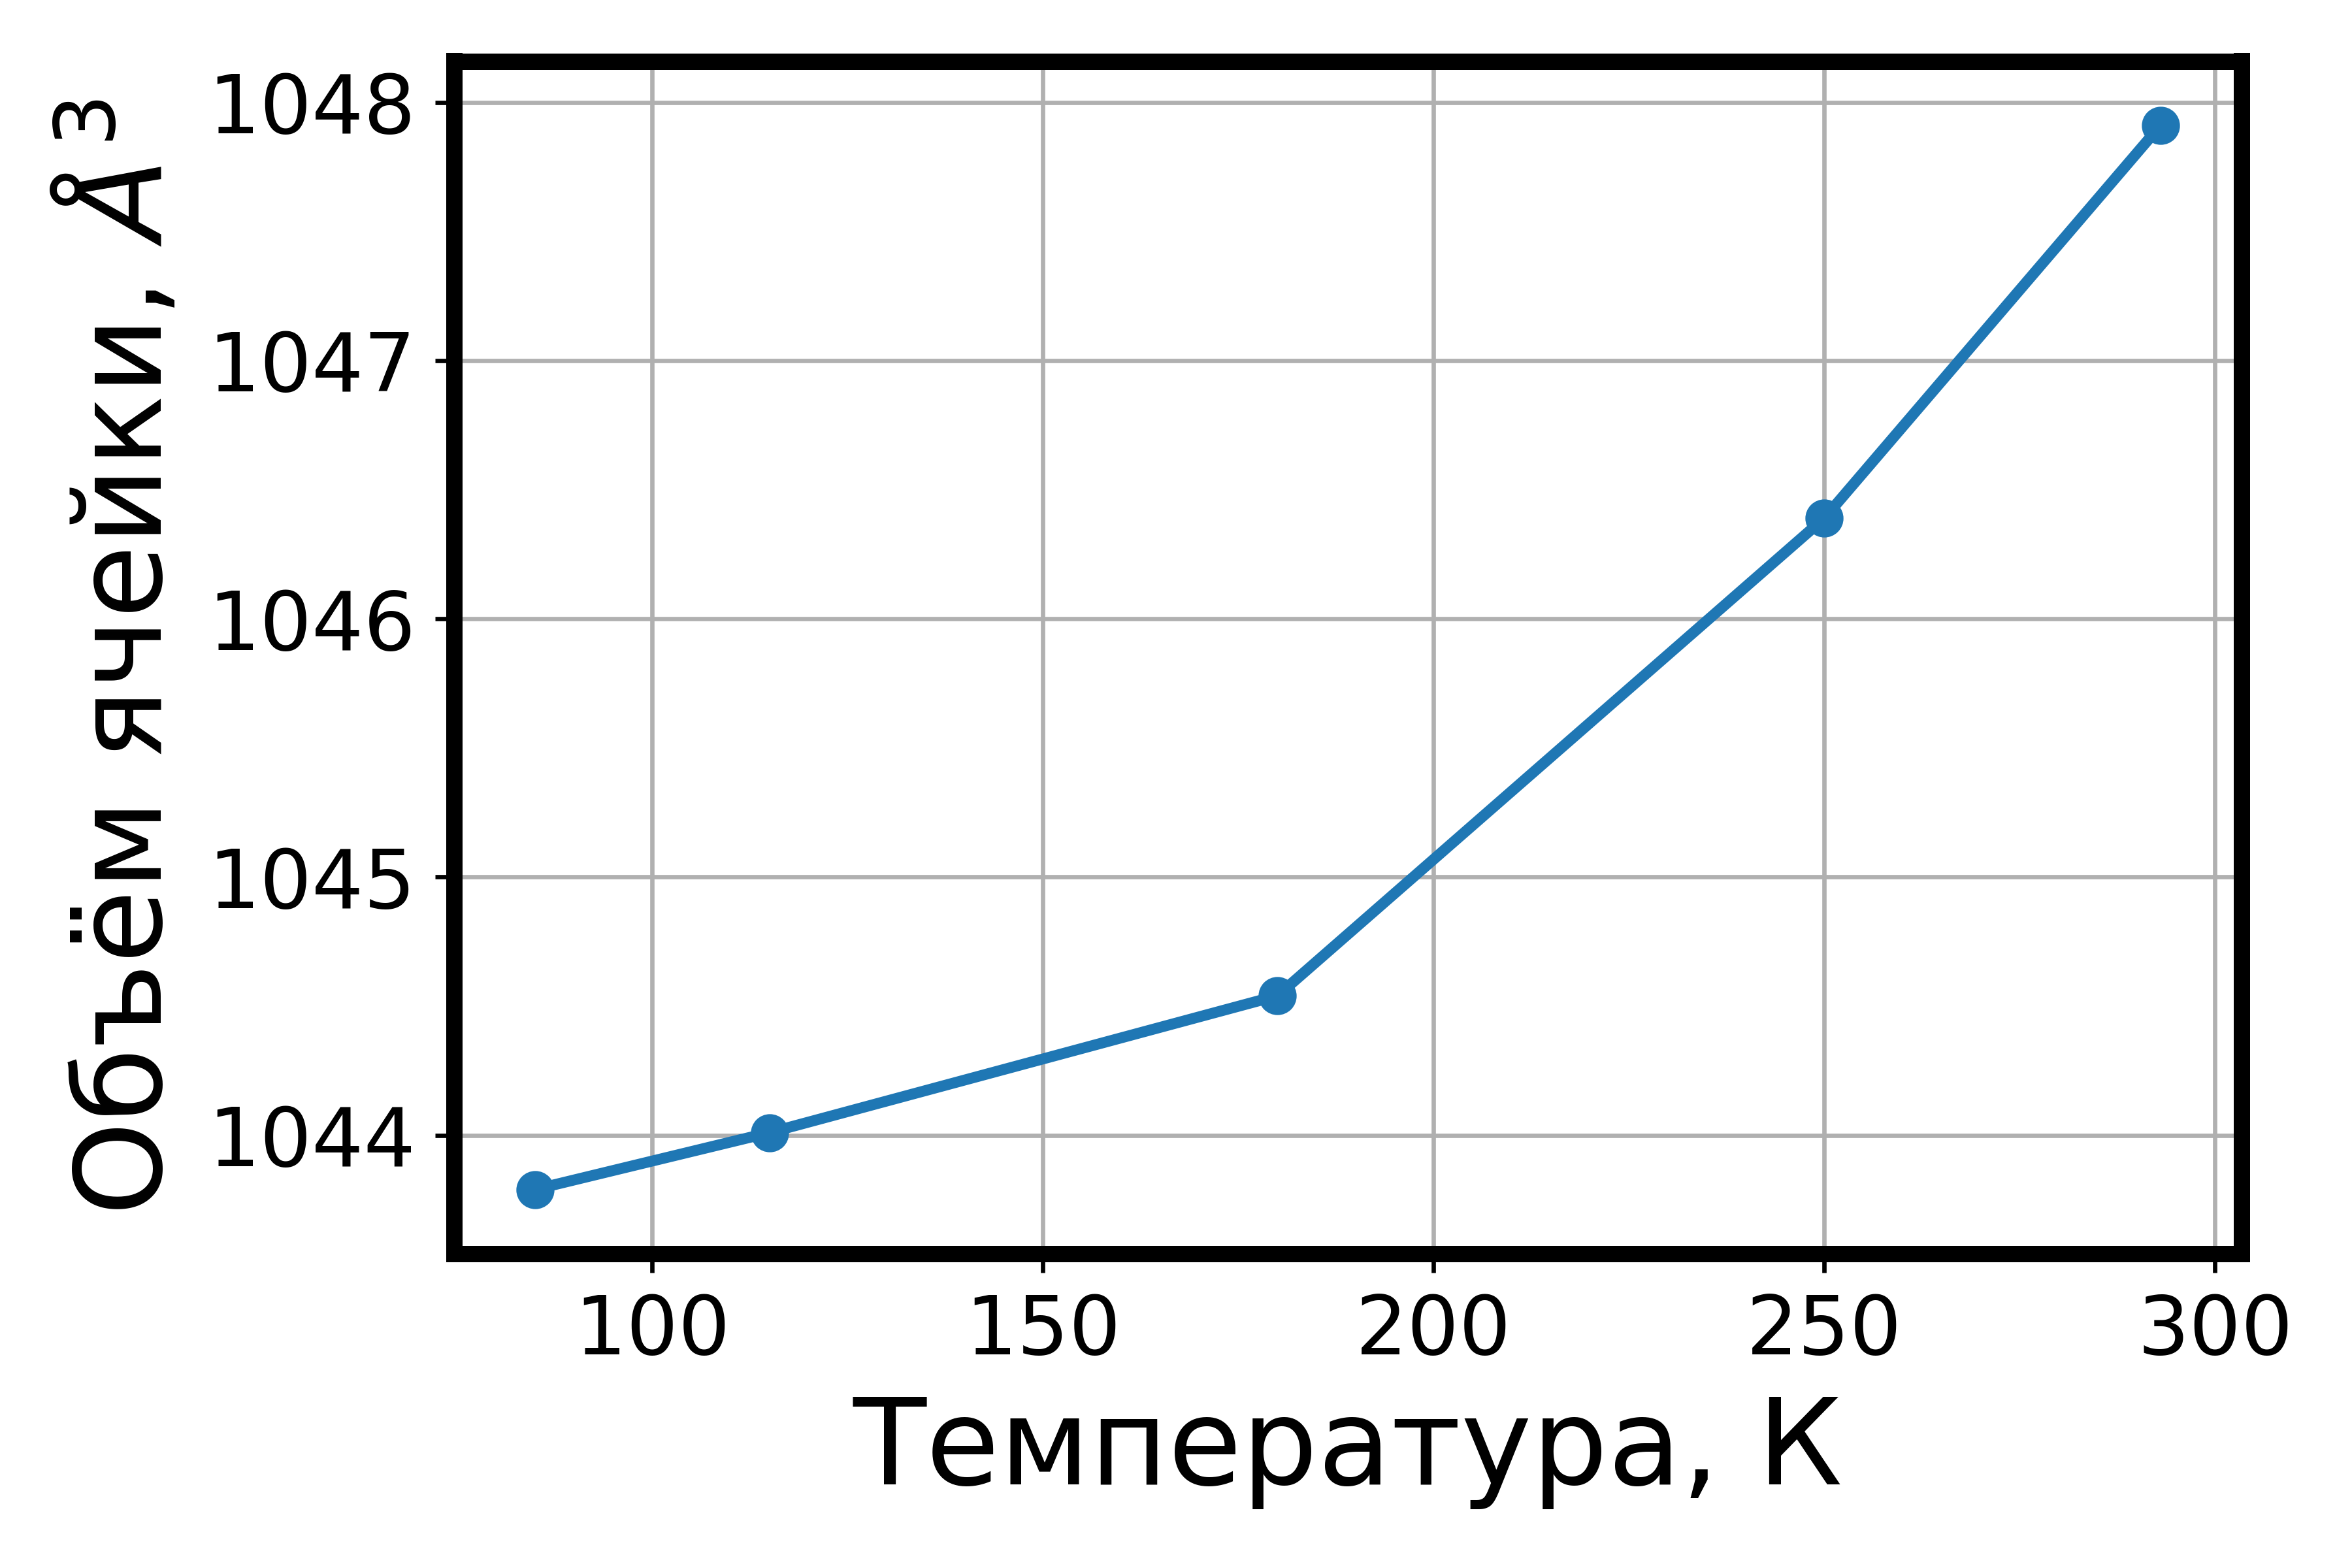
\includegraphics[width=0.9\linewidth]{structure_volume} \\ б)
  \end{minipage}

      \caption[Графики зависимости изменения заселённости для позиции Cu21(а) и объёма кристаллической решетки (б) образца синтетического теннантита Cu\textsubscript{12}As\textsubscript{4}S\textsubscript{13} при температурах 85, 115, 180, 250 и 293~К]{Графики зависимости изменения заселённости для позиции Cu21 (а) и объёма кристаллической решетки(б) образца синтетического теннантита Cu\textsubscript{12}As\textsubscript{4}S\textsubscript{13} при температурах 85, 115, 180, 250 и 293~К}
    \label{img:structure1}
\end{figure}

\begin{figure}[p!]
  \begin{minipage}[ht]{0.9\linewidth}\centering
    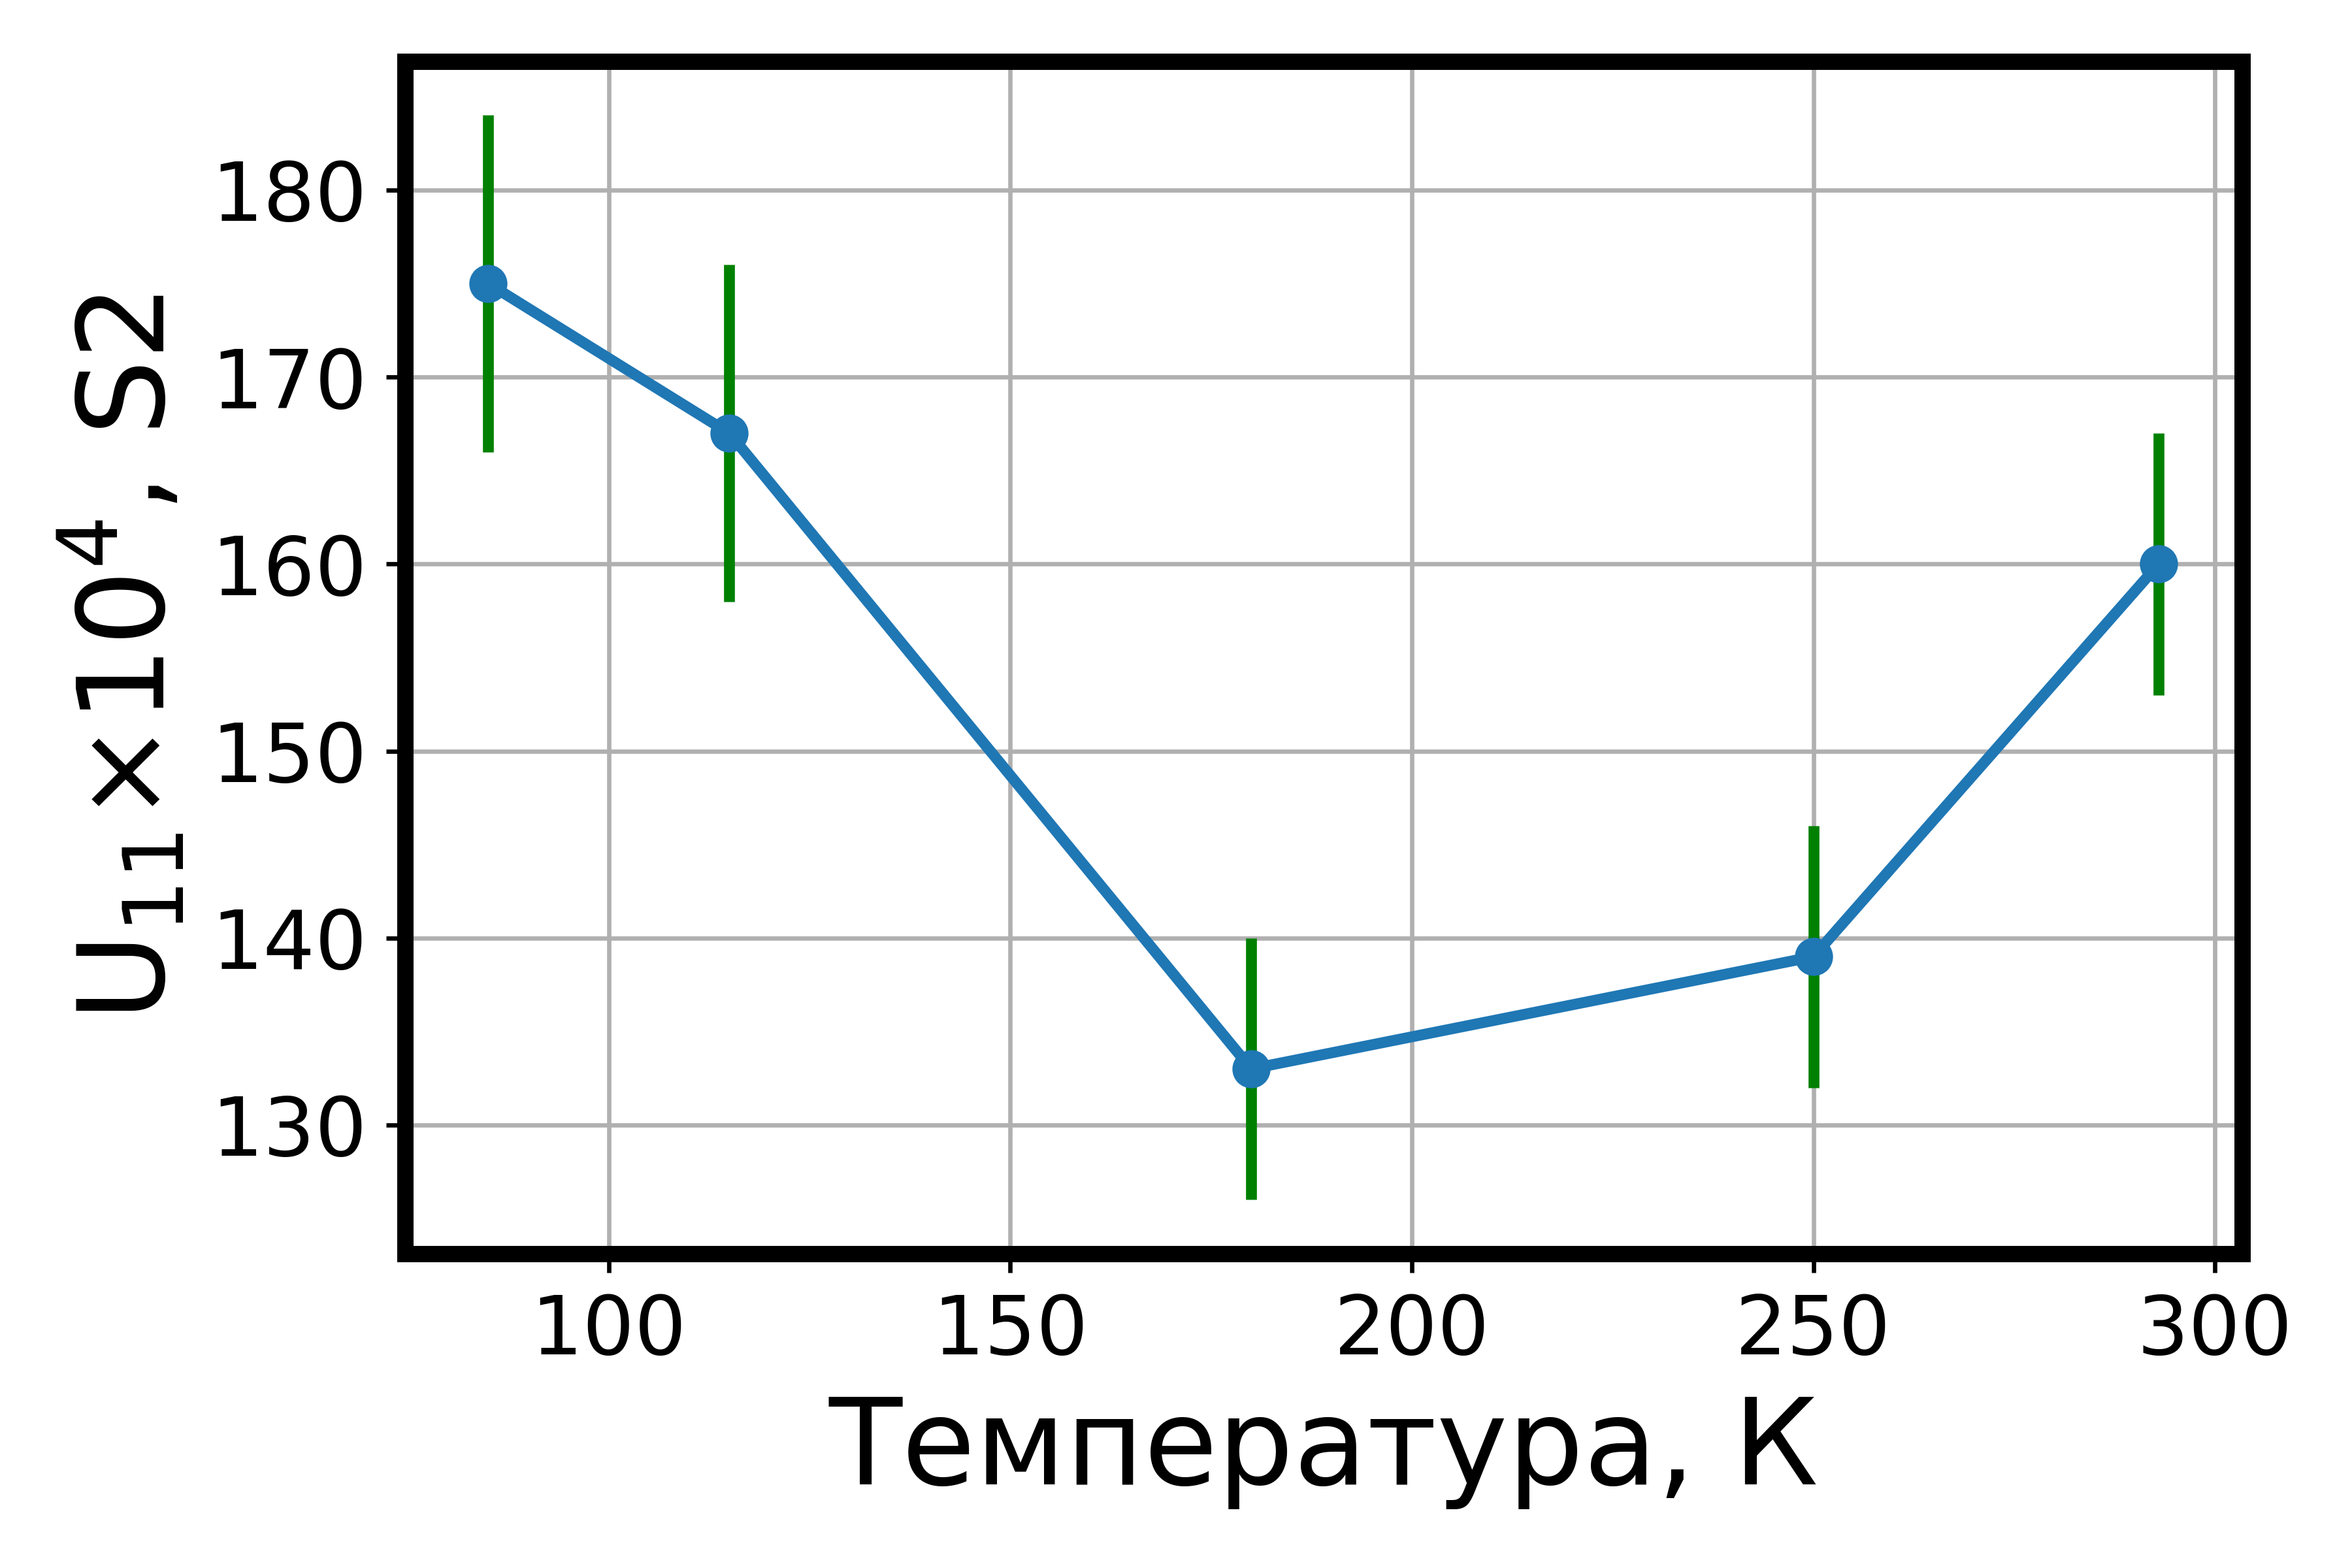
\includegraphics[width=0.9\linewidth]{structure_Ueq} \\ а)
  \end{minipage}
  \vfill
  \begin{minipage}[ht]{0.9\linewidth}\centering
    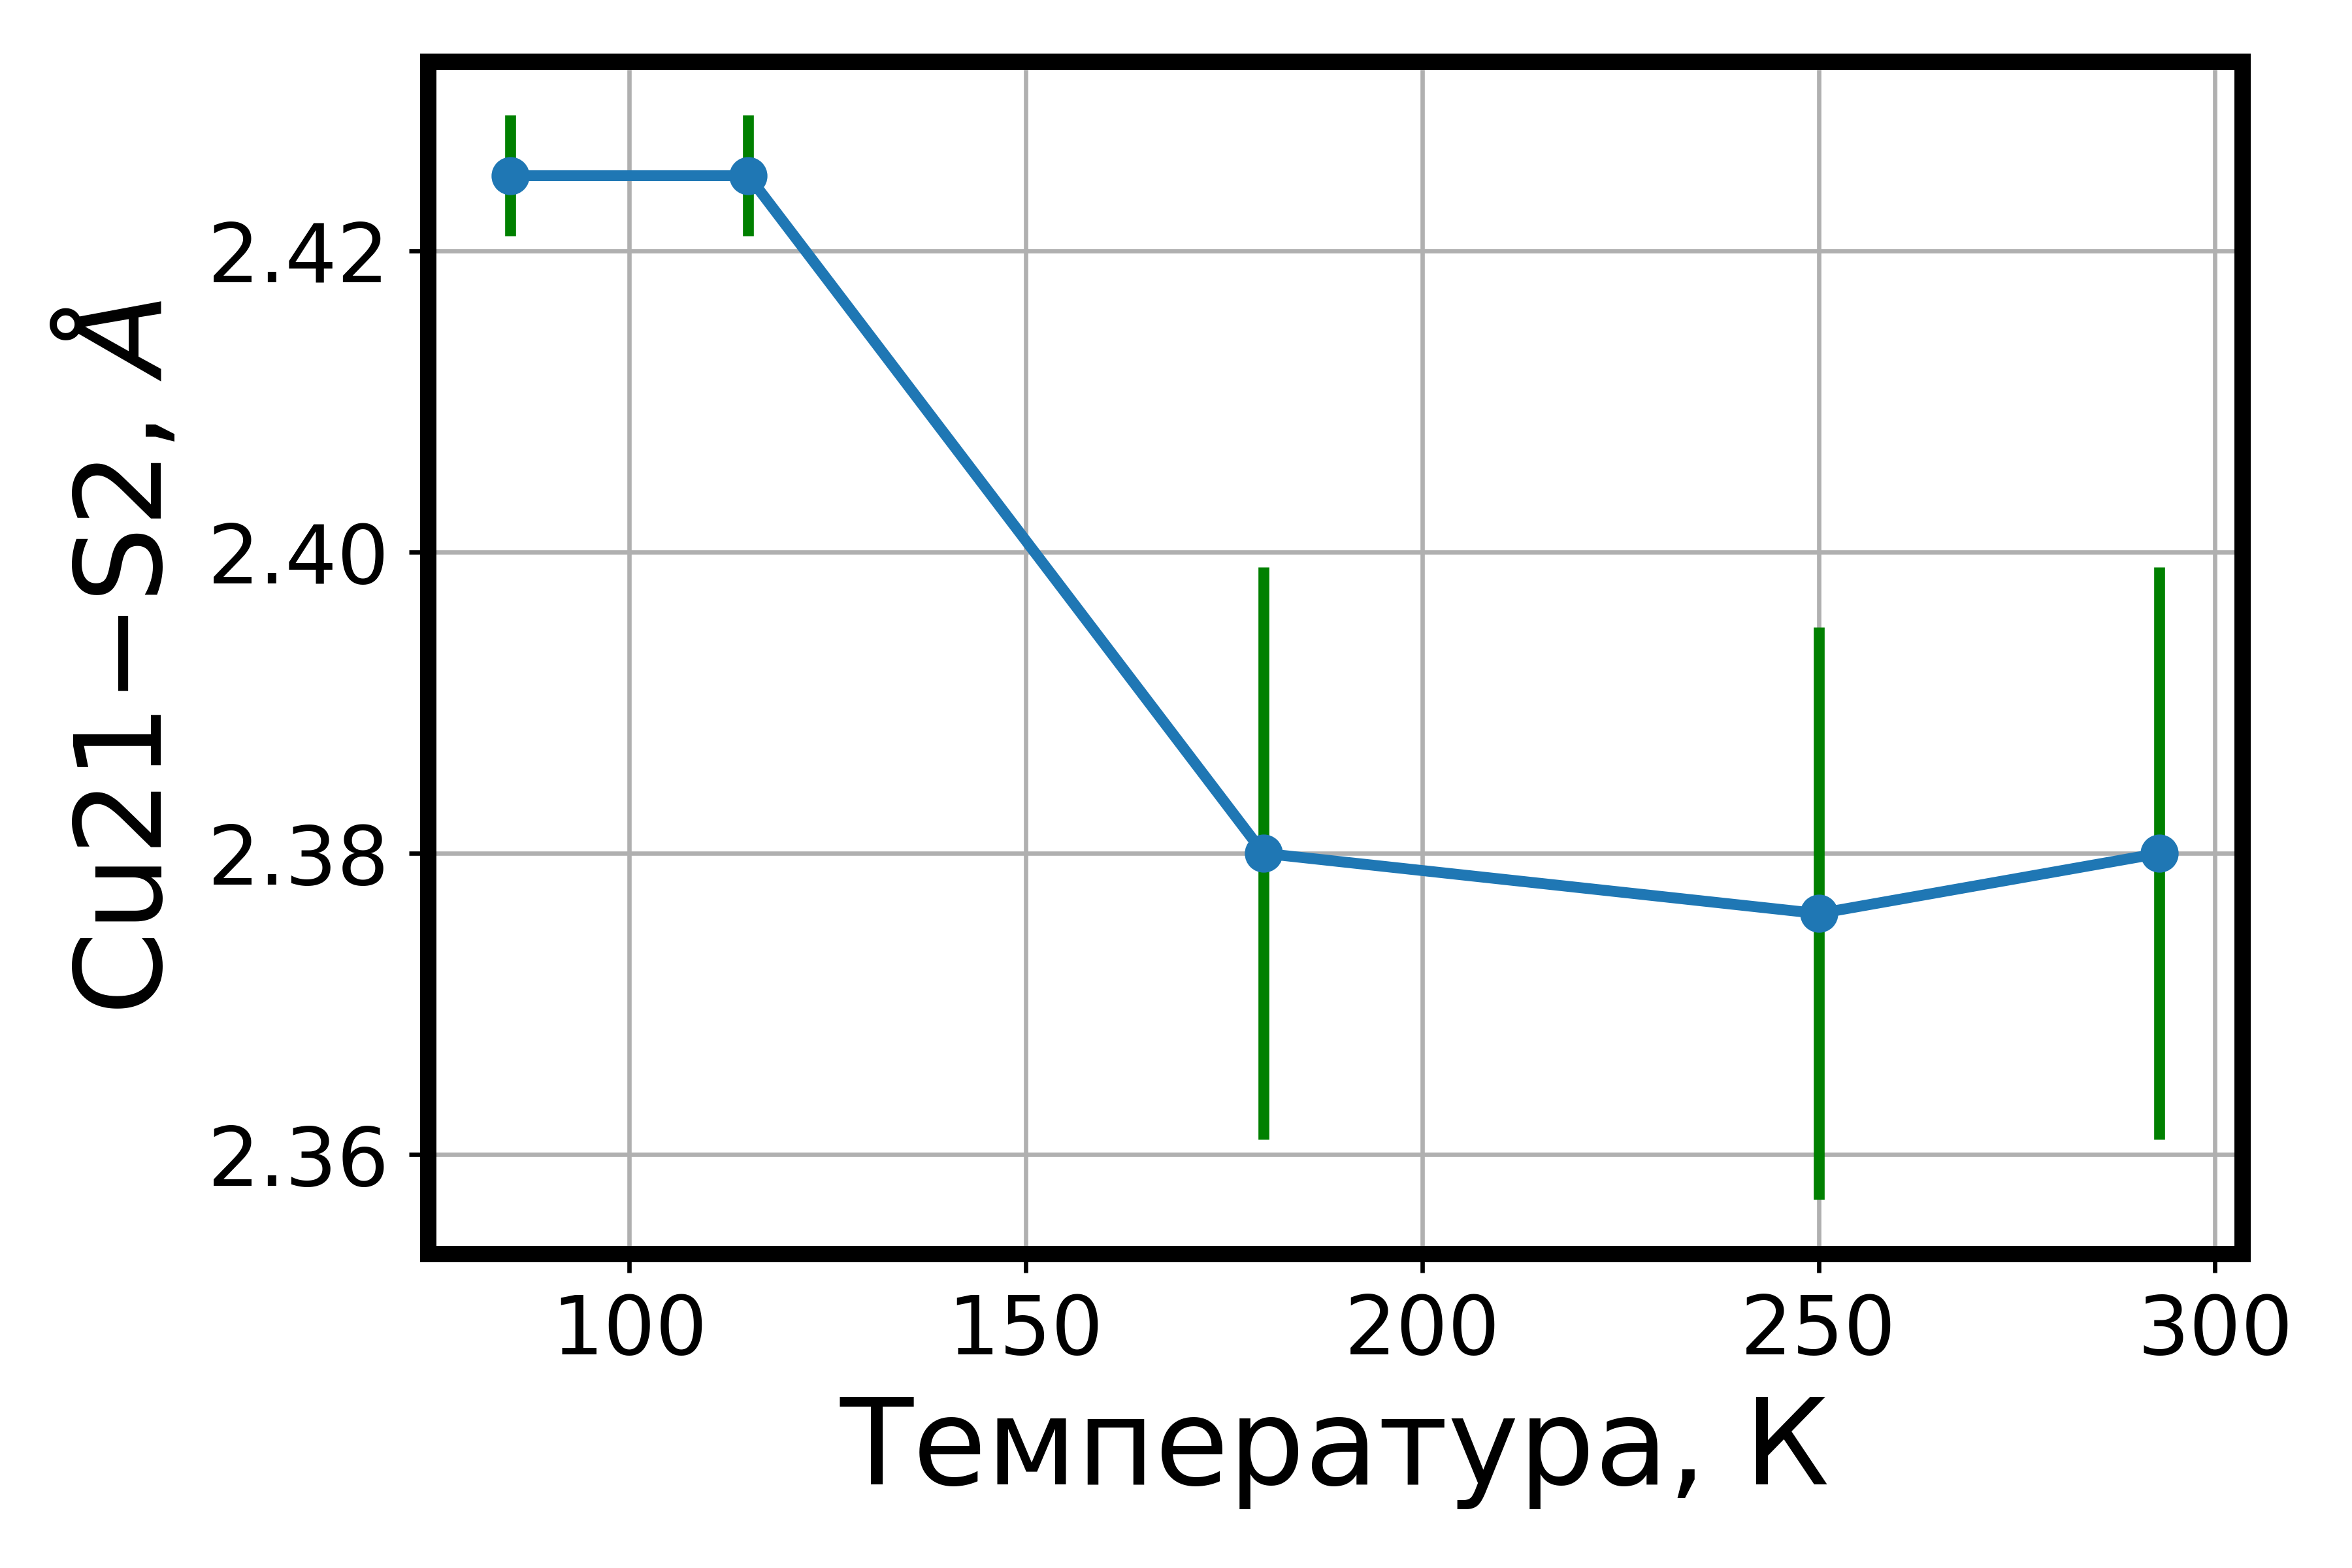
\includegraphics[width=0.9\linewidth]{structure_cu21_s2} \\ б)
  \end{minipage}

      \caption[Графики зависимостей атомарного смещения U\textsubscript{11} (а) и расстояния между позициями Cu21--S2 (б) для образца синтетического теннантита Cu\textsubscript{12}As\textsubscript{4}S\textsubscript{13} при температурах 85, 115, 180, 250 и 293~К]{Графики зависимостей атомарного смещения U\textsubscript{11} (а) и расстояния между позициями Cu21--S2 (б) для образца синтетического теннантита Cu\textsubscript{12}As\textsubscript{4}S\textsubscript{13} при температурах 85, 115, 180, 250 и 293~К}
    \label{img:structure2}
\end{figure}
\newpage

\section{Электронная просвечивающая микроскопия монокристаллического образца синтетического теннантита Cu\textsubscript{12}As\textsubscript{4}S\textsubscript{13} в плоскости (011) } \label{sect3_2}

Исследования особенностей распределения меди в образце проведены при комнатной температуре на образце толщиной менее 100~нм для кристаллографической плоскости (011).
Установлено, что в образце синтетического теннантита Cu\textsubscript{12}As\textsubscript{4}S\textsubscript{13} есть различия значения эллиптичности в рядах меди Cu (Рис. \ref{img:mic}).

\begin{figure}[h!]
  \begin{minipage}[ht]{0.9\linewidth}\centering
    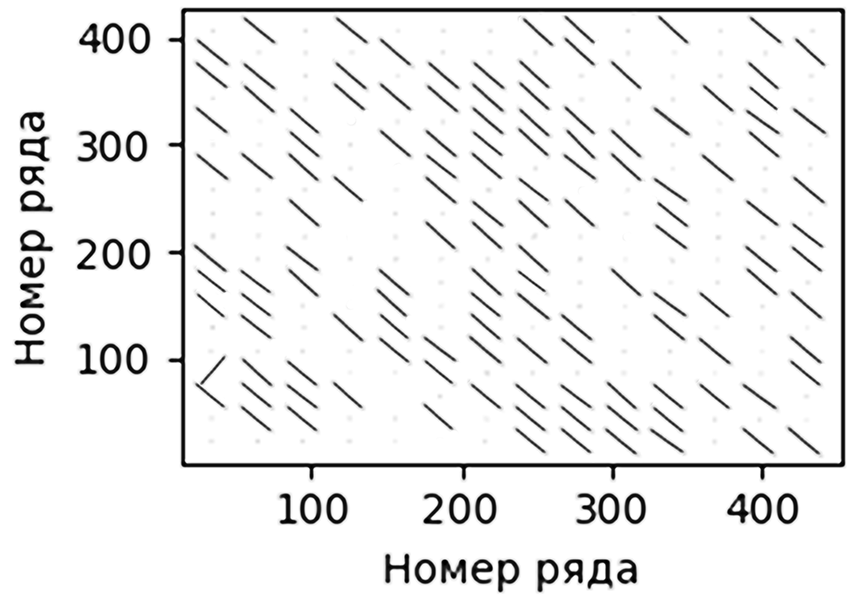
\includegraphics[width=0.7\linewidth]{mic_cupper_raw}
  \end{minipage}

      \caption[Величина и разворот эллиптичности рядов Cu в кристаллографической плоскости (011) синтетического теннантита Cu\textsubscript{12}As\textsubscript{4}S\textsubscript{13}]{Величина и разворот эллиптичности рядов Cu в кристаллографической плоскости (011) синтетического теннантита Cu\textsubscript{12}As\textsubscript{4}S\textsubscript{13}}
    \label{img:mic}
\end{figure}


На рисунке \ref{img:mic2} электронная дифракция для плоскости (011) образца синтетического образца Cu\textsubscript{12}As\textsubscript{4}S\textsubscript{13}.
Дифракция обладает отлично определяемыми пиками, которые хорошо идентифицируются (рис. \ref{img:mic2}(б)).

\begin{figure}[ph!]
\centering
  \begin{minipage}[ht]{0.7\linewidth}\centering
    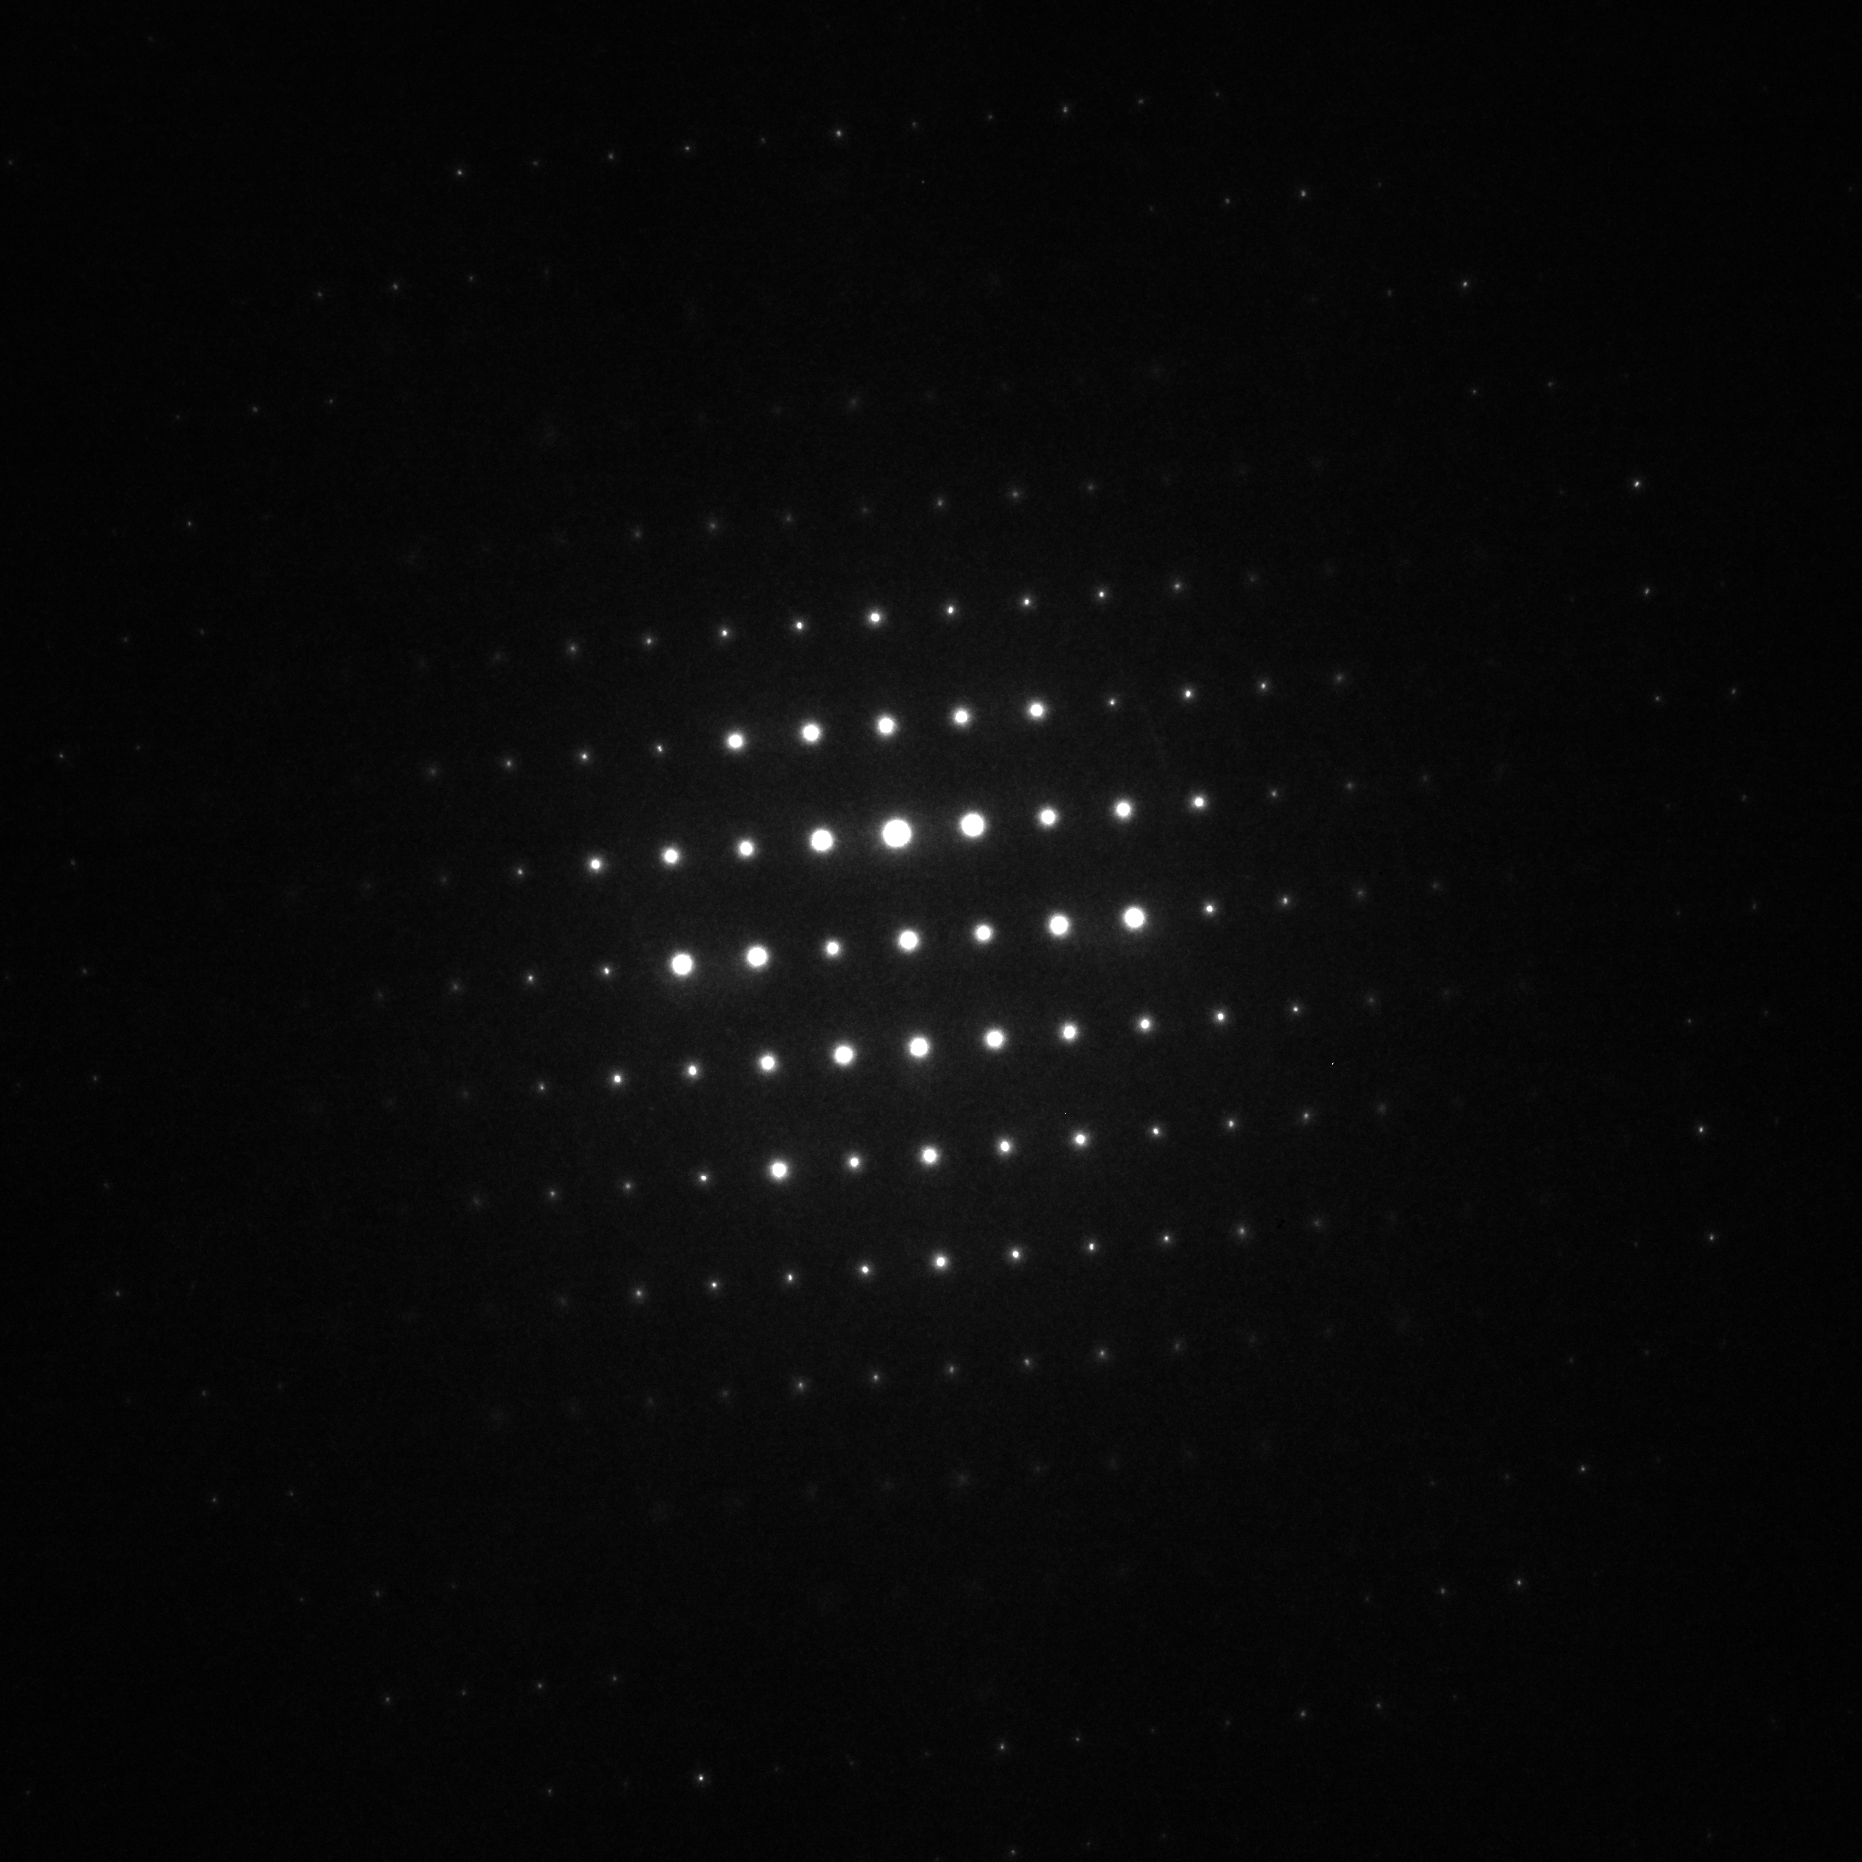
\includegraphics[width=0.9\linewidth]{difr01_el_mic} \\ а)
  \end{minipage}
  \vfill
  \begin{minipage}[ht]{0.7\linewidth}\centering
    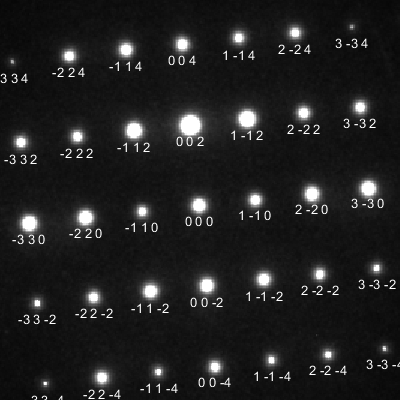
\includegraphics[width=0.9\linewidth]{difr01_el_mic_zone_110} \\ б)
  \end{minipage}
  \caption[Электронная дифракция для плоскости (011) для образца Cu\textsubscript{12}As\textsubscript{4}S\textsubscript{13}. Оригинальное изображение (а) и изображение с отмеченными дифракционными рефлексами (б)]{Электронная дифракция для плоскости (011) для образца Cu\textsubscript{12}As\textsubscript{4}S\textsubscript{13}. Оригинальное изображение (а) и изображение с отмеченными дифракционными рефлексами (б)}
    \label{img:mic2}
\end{figure}

Анализ изображения структуры показывает наличие разной эллиптичности для рядов атомов меди. На рисунке \ref{img:mic} представлено наличие эллиптичности атомов рядов меди с учётом дрейфа для плоскости (011) синтетического теннантита Cu\textsubscript{12}As\textsubscript{4}S\textsubscript{13}.




\newpage



\section{Комбинационное рассеяние света синтетического теннантита Cu\textsubscript{12}As\textsubscript{4}S\textsubscript{13}} \label{sect3_3}

Спектр комбинационного рассеяния для синтетического теннантита обладает низкоэнергетическими модами (Рис. \ref{img:raman1a}).

Спектр комбинационного рассеяния света состоит из следующих пиков: $\nu_{1}$, $\nu_{2}$, $l_{1}$, $l_{2}$ на 374.5, 340, 64, и 122 см\textsuperscript{-1} соответсвенно и широкого пика $\nu_{4}$ на 320 см\textsuperscript{-1}. Пики между 200 и 400 см\textsuperscript{-1} относят к модам от (Sb, As)S\textsubscript{3}\cite{Kharbish2007}. Позиция пика $\nu_{3}$ найдена методом наименьших квардатов с помощью пакета LMFIT.
Результаты моделирования представлены пунктиром на Рис. \ref{raman_25_CuAsS3_rus_components}. 
Определенные по экспериментальным спектрам положения и полуширина пиков ниже 200 см\textsuperscript{-1} для синтетического теннантита составляют 62(14) и 122(24) см\textsuperscript{-1}.  По мнению авторов \cite{Buzatu2017}, эти моды связываны с особенностями динамики кристаллической решетки.

Определение положения  и  полуширины пика проведено с помощью функции псевдо-Фойгта, а фон описывался полиномной функцией.

\begin{figure}[h]
    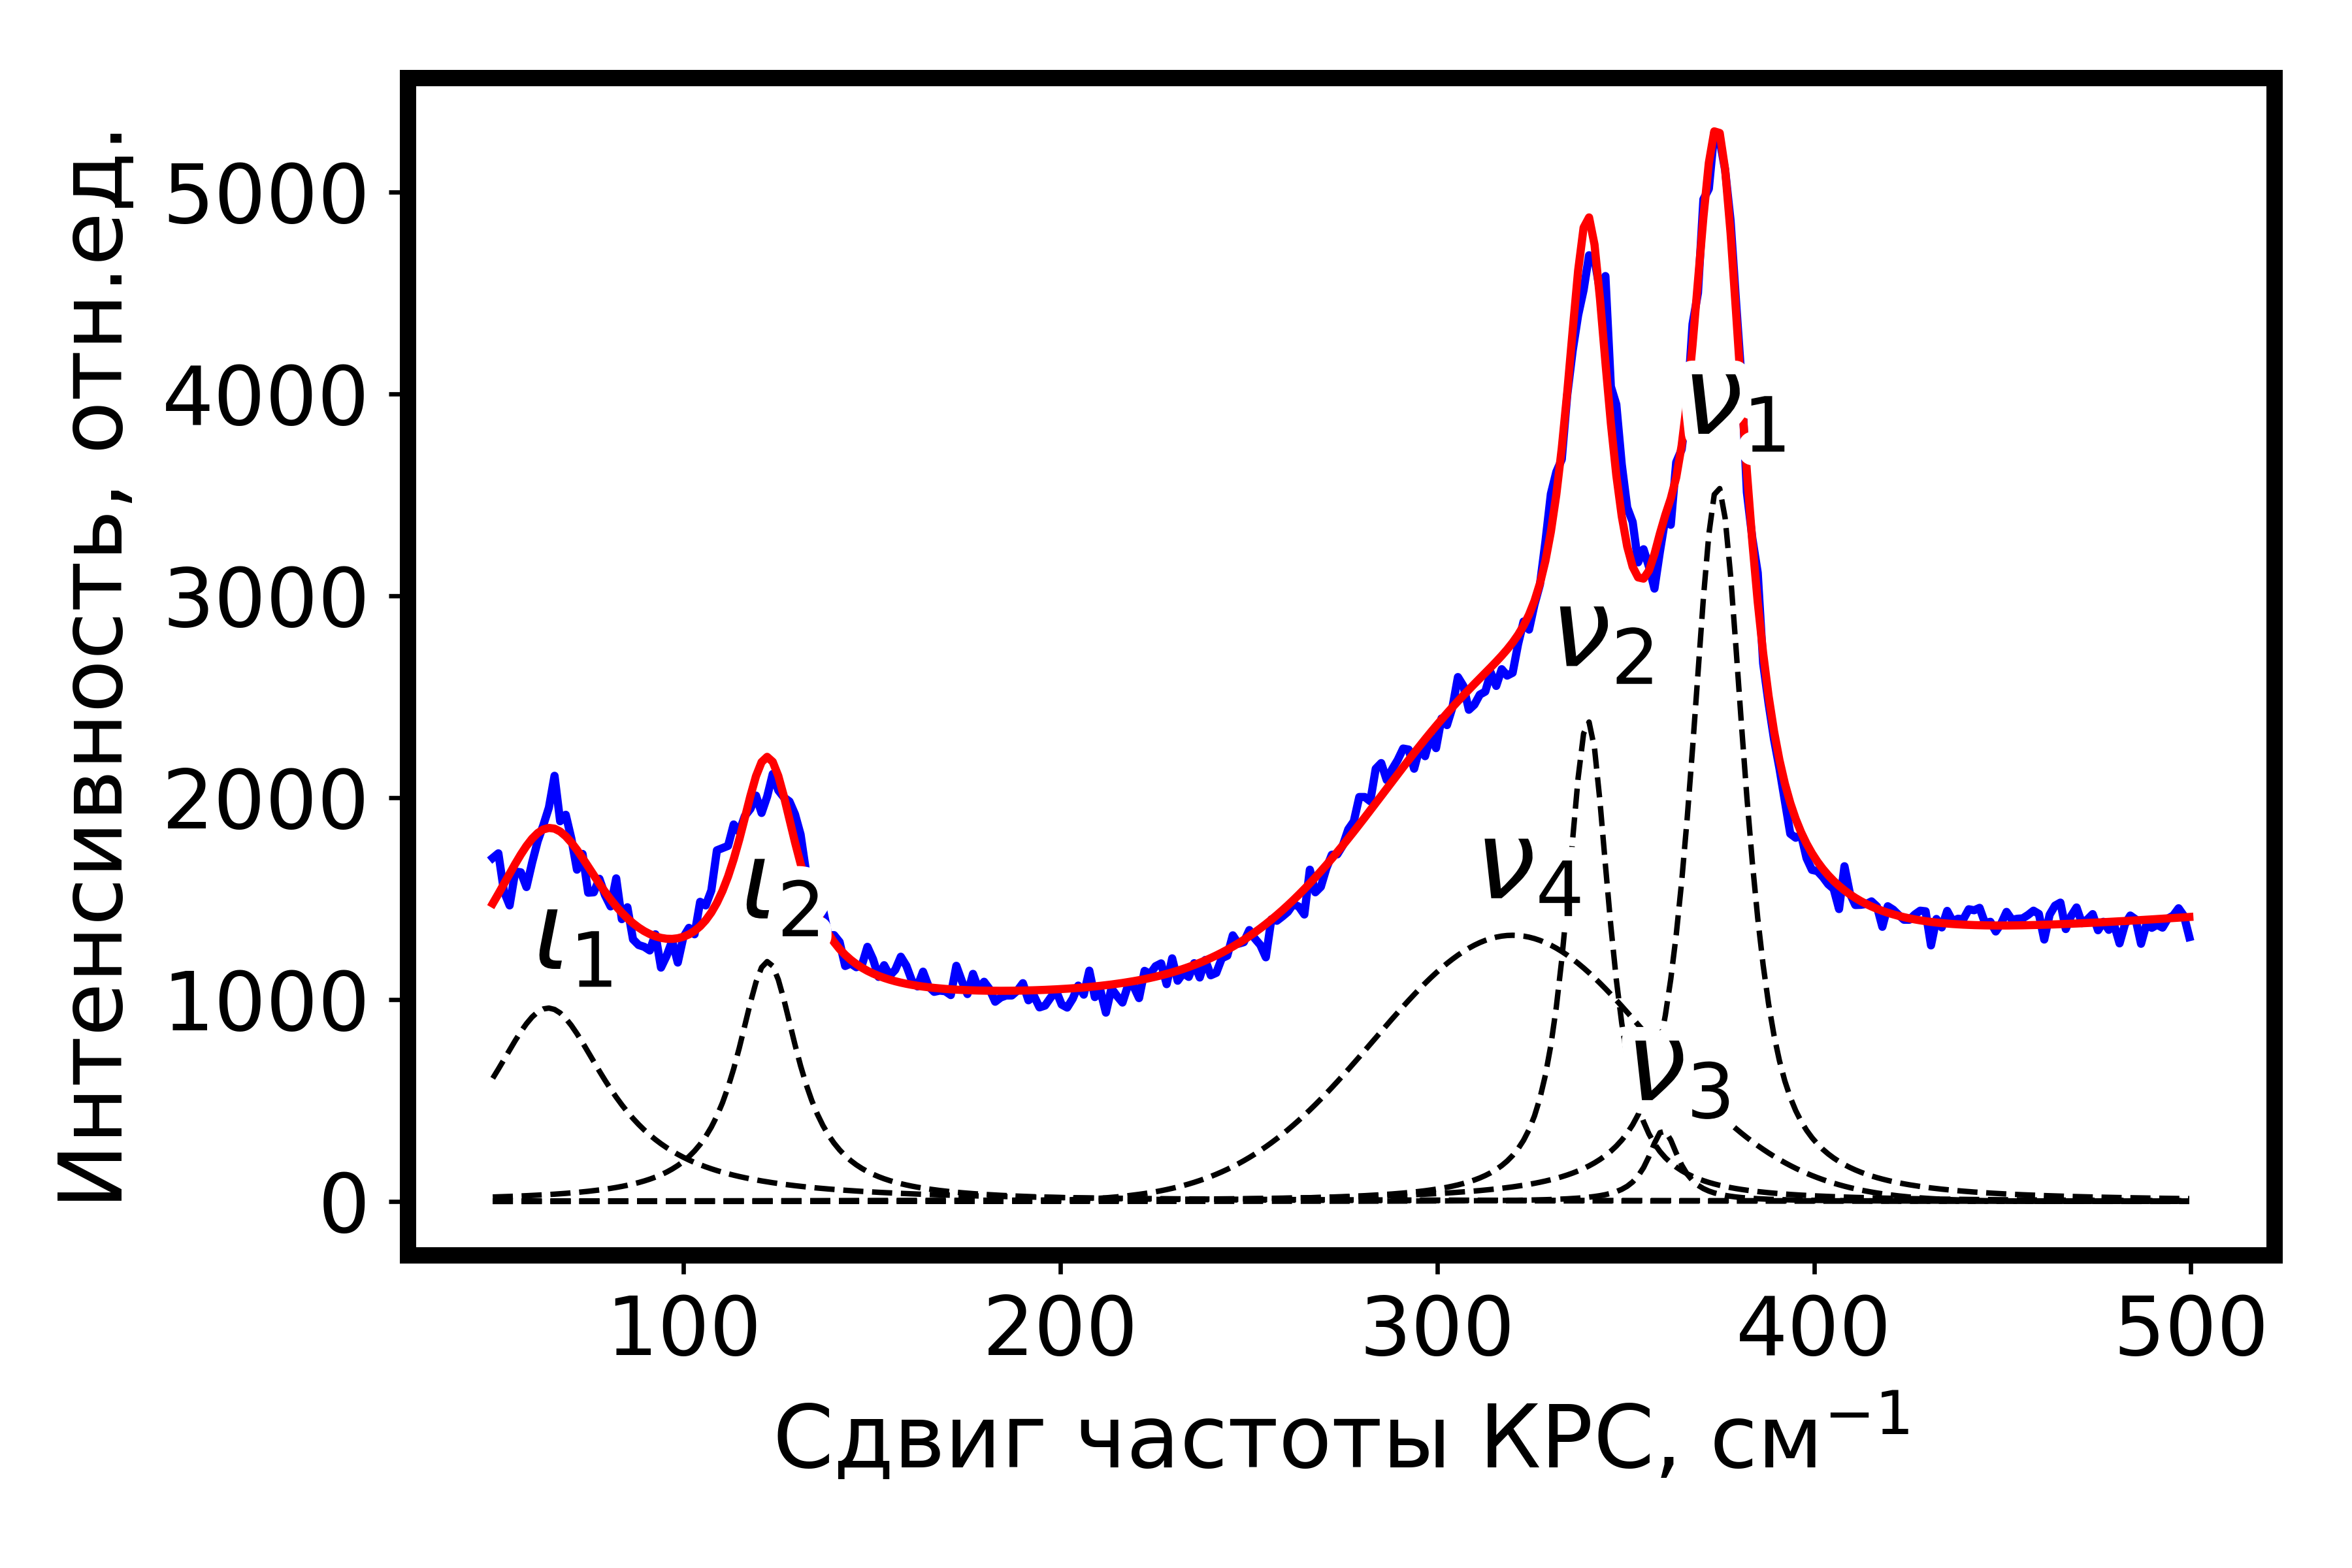
\includegraphics[width=0.9\linewidth]{raman_25_CuAsS3_rus_components}

      \caption[График спектра комбинационного рассеяния синтетического теннатита Cu\textsubscript{12}As\textsubscript{4}S\textsubscript{13}]{График спектра комбинационного рассеяния синтетического теннатита Cu\textsubscript{12}As\textsubscript{4}S\textsubscript{13}}

    \label{img:raman1a}
\end{figure}

\newpage


\section{Квантовомеханические расчёты структур синтетического теннантиа Cu\textsubscript{12}As\textsubscript{4}S\textsubscript{13}} \label{sect3_4}

Для исследования наиболее выгодного положения атомов меди были рассчитаны энергии 20 структур с разным положением атомов меди.
Структуры разделены на две группы: первая --- в лавесовском полиэдре сдвинуты 6 атомов меди (структуры с 1 по 10), вторая --- сдвинуты 3 атома меди в лавесовском полиэдре (структуры с 10 по 19). Изображения рассчитанных структур представлены на рисунках \ref{img:laves1}, \ref{img:laves2}, \ref{img:laves3} и \ref{img:laves4}.
На рисунке \ref{img:th} изображен график со значениями энергий элементарных ячеек для рассчитанных структур. Красной пунктирной линией обозначена энергия исходной структуры.
Экспериментальные структуры, полученные после анализа рентгеноструктурных экспериментов при разных температурах, были рассчитаны с учетом ферромагнитного, антиферромагнитного, парамагнитного (ПМ) и диамагнитного состояний в структурах.
Антиферромагнитное упорядочение в экспериментальной структуре при 85~К энергетически более выгодно, чем ферро- или пара- или диамагнитное состояния. При этом для 293~К ФМ, АФМ, ПМ конфигурации имеют одинаковую (до 4 знака) энергию, что указывает на их одинаковую выгодность.

\begin{figure}[ht!]
  \begin{minipage}[ht]{0.9\linewidth}\centering
    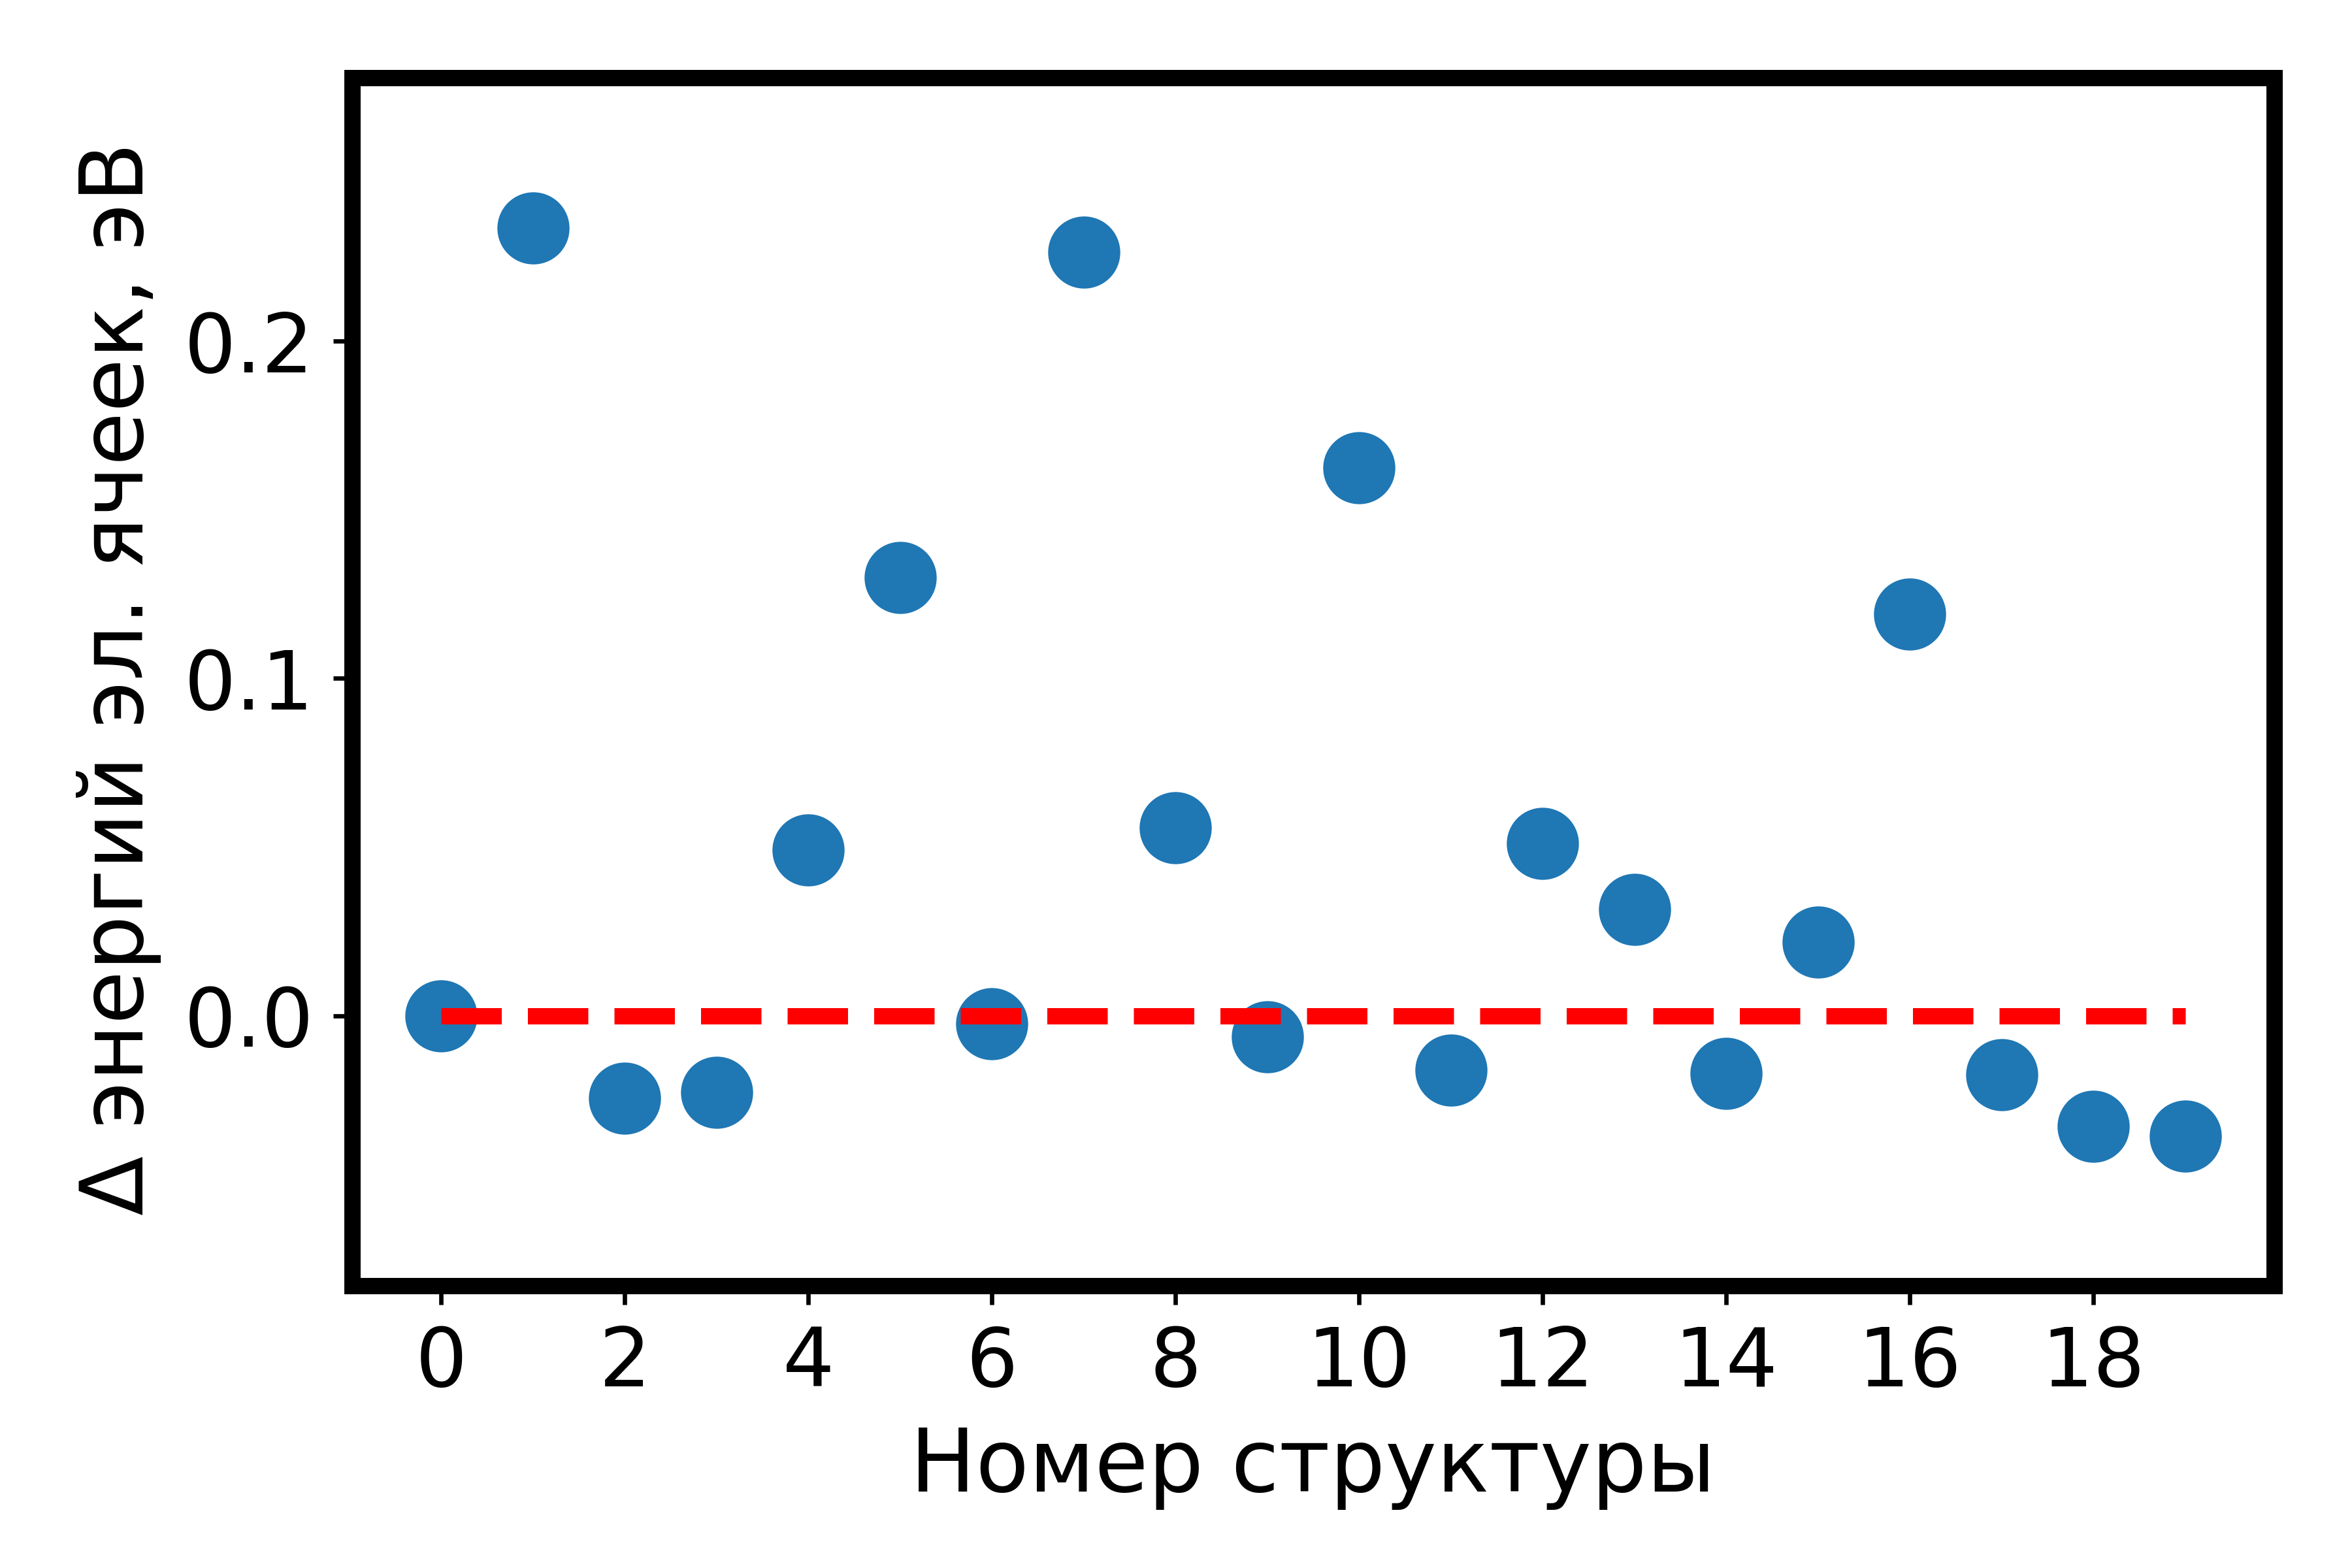
\includegraphics[width=0.7\linewidth]{energy_structure}
  \end{minipage}

      \caption[Сводный график энергий рассчитанных структур относительно энергии исходной структуры с разным расположением атомов в лавесовском полиэдре]{Сводный график энергий рассчитанных структур относительно энергии исходной структуры с разным расположением атомов в лавесовском полиэдре}
    \label{img:th}
\end{figure}

\begin{landscape}
\begin{table} [htbp]
\centering

\caption{Сводная таблица распределения электрических зарядов для рассчитанных структур (варианты с 0 по 9 включительно) с разным расположением атомов меди в лавесовском полиэдре для синтетического теннантита Cu\textsubscript{12}As\textsubscript{4}S\textsubscript{13}}%
	\label{mod_char1}% label всегда желательно идти после caption
    \renewcommand{\arraystretch}{1.5}
	%\resizebox{\textwidth}{!}{
    \begin{tabular}{@{}@{\extracolsep{10pt}}lllllllllll@{}}
      \toprule     %%% верхняя линейка
Atom & Var0          & Var1          & Var2          & Var3          & Var4   & Var5          & Var6          & Var7          & Var8          & Var9              \\  \midrule
Cu1                  & +0.57	                & +0.56	                  & {\bf +0.56 }	& {\bf +0.56 }	& +0.56	& +0.56	                  & +0.56	& +0.56	& +0.56	                  & {\bf +0.56} \\
\multirow{2}{*}{Cu2} & \multirow{2}{*}{+0.49}	& \multirow{2}{*}{+0.47}	& {\bf +0.45 }	& {\bf +0.49 }	& +0.47 & +0.51	                  & +0.49	& +0.49	& +0.49	                  & {\bf +0.50} \\
		                 &		                    &                         & {\bf +0.40 }	& {\bf +0.39 }	& +0.40	& +0.47	                  & +0.39	& +0.39	& +0.45	                  & {\bf +0.46} \\
\multirow{2}{*}{S1}  & -1.41	                & -1.45	                  & {\bf -1.42 }  & {\bf -1.42 }	& -1.39	& \textcolor{red}{-0.76}	& -1.43	& -1.43	& \textcolor{blue}{-0.73}	& \textcolor{blue}{-0.70} \\
                     & -1.47	                & -1.53	                  & {\bf -1.49 }  & {\bf -1.50 }	& -1.47	& \textcolor{red}{-0.92}	& -1.53	& -1.52	& \textcolor{blue}{-1.42}	& \textcolor{blue}{-1.44} \\
S2                   & -0.88	                & -0.85	                  & {\bf -0.78 }  & {\bf -0.82 }	& -0.84	& -0.84	                  & -0.83	& -0.83	& -0.86	                  & {\bf -0.86} \\
\multirow{2}{*}{As}  & \multirow{2}{*}{+2.97}	& +3.05	                  & {\bf +3.12 }	& {\bf +3.15 }	& +3.06	& +0.86	                  & +3.11	& +3.12	& \textcolor{blue}{+2.03}	& \textcolor{blue}{+1.51} \\
	                   &                        & +2.99	                  & {\bf +2.99 }  & {\bf +3.07 }	& +3.11	& +0.93	                  & +3.06	& +3.07	& \textcolor{blue}{+1.53}	& \textcolor{blue}{+0.89} \\
\bottomrule

\end{tabular}
%}
\end{table}
\end{landscape}

\begin{landscape}
\begin{table} [htbp]
\centering
\caption{Сводная таблица распределения электрических зарядов для рассчитанных структур (варианты с 10 по 19 включительно) с разным расположением атомов меди в лавесовском полиэдре для синтетического теннантита Cu\textsubscript{12}As\textsubscript{4}S\textsubscript{13}}%
	\label{mod_char2}% label всегда желательно идти после caption
    \renewcommand{\arraystretch}{1.5}
	\begin{tabular}{@{}@{\extracolsep{10pt}}lllllllllll@{}}

\toprule     %%% верхняя линейка
Atom                         &Var10& Var11& Var12& Var13 & Var14& Var15& Var16& Var17& Var18& Var19          \\ \hline
Cu1                  & +0.56   & 	{\bf +0.56 }           & 	+0.56  & 	+0.56                  & 	{\bf +0.56 }           & 	+0.56                  & 	+0.56                  & 	{\bf +0.56 }           & 	{\bf +0.56 }           & 	{\bf +0.56 } \\
\multirow{2}{*}{Cu2} & +0.48   & 	{\bf +0.51 }           & 	+0.46  & 	+0.51                  & 	{\bf +0.50 }           & 	+0.51                  & 	+0.51                  & 	{\bf +0.51 }           & 	{\bf +0.51 }           & 	{\bf +0.50 } \\
		                 & +0.39   & 	{\bf +0.48 }           & 	+0.45  & 	+0.47                  & 	{\bf +0.46 }           & 	+0.46                  & 	+0.45                  & {\bf +0.46 }            & 	{\bf +0.46 }           & 	{\bf +0.46 } \\
\multirow{2}{*}{S1}  & -1.43   & 	\textcolor{red}{-0.73} & 	-1.42  & 	\textcolor{red}{-0.72} & 	\textcolor{red}{-0.73} & 	\textcolor{red}{-0.73} & 	\textcolor{red}{-0.72} & 	\textcolor{red}{-0.72} & 	\textcolor{red}{-0.74} & 	\textcolor{red}{-0.72} \\
                     & -1.52   & 	\textcolor{red}{-0.76} & 	-1.52  & 	\textcolor{red}{-0.77} & 	\textcolor{red}{-0.76} & 	\textcolor{red}{-0.77} & 	\textcolor{red}{-0.77} & 	\textcolor{red}{-0.77} & 	\textcolor{red}{-0.76} & 	\textcolor{red}{-0.76} \\
S2                   & -0.82   & 	{\bf -0.98}            & 	-0.81  & 	-0.93                  & 	{\bf -0.90 }           & 	-0.94                  & 	-0.90                  & 	{\bf -0.88 }           & 	{\bf -0.91 }           & 	{\bf -0.89 } \\
\multirow{2}{*}{As}  & +3.11   & 	\textcolor{red}{+0.94} & 	+3.07  & \textcolor{red}{+0.94}  & 	\textcolor{red}{+0.94} & 	\textcolor{red}{+0.94} & 	\textcolor{red}{+0.95} & 	\textcolor{red}{+0.95} & 	\textcolor{red}{+0.91} & 	\textcolor{red}{+0.91} \\
	                   & +3.00	 & \textcolor{red}{+0.76}	 & +2.99	 & \textcolor{red}{+0.85}	 & \textcolor{red}{+0.80}	 & \textcolor{red}{+0.84}	 & \textcolor{red}{+0.87}	 & \textcolor{red}{+0.85}	 & \textcolor{red}{+0.85}	 & \textcolor{red}{+0.84} \\
 \bottomrule


\end{tabular}
\end{table}
\end{landscape}

\begin{figure}[p!]
  \begin{minipage}[ht]{0.45\linewidth}\centering
    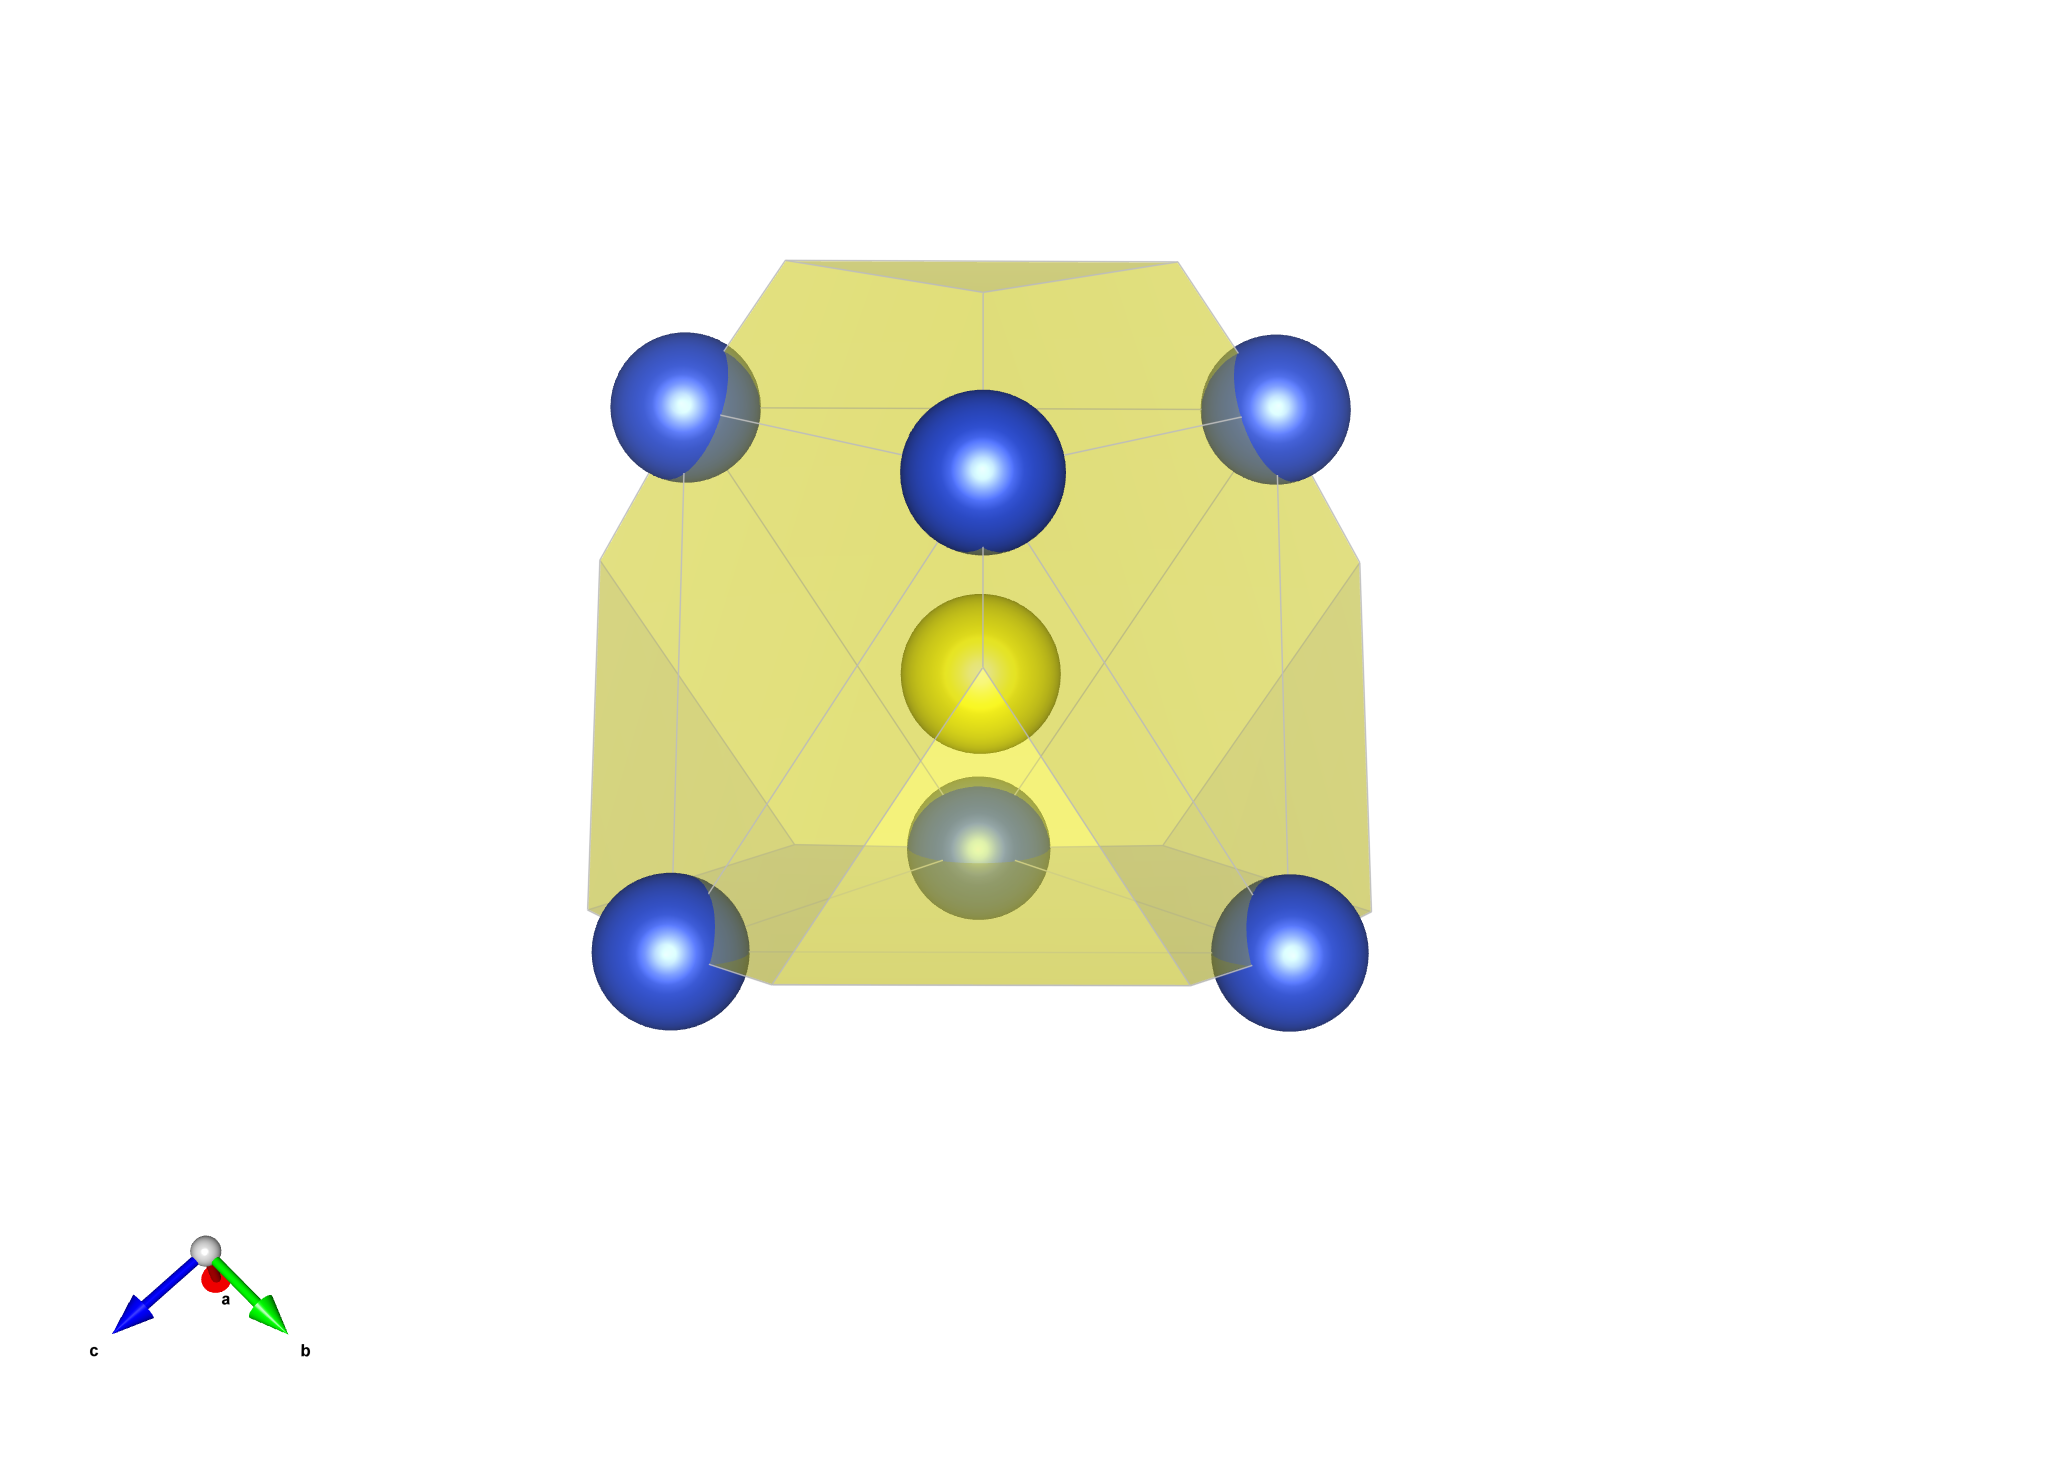
\includegraphics[width=0.9\linewidth]{var_0} \\ а)
  \end{minipage}
						\hfill
 \begin{minipage}[ht]{0.45\linewidth}\centering
    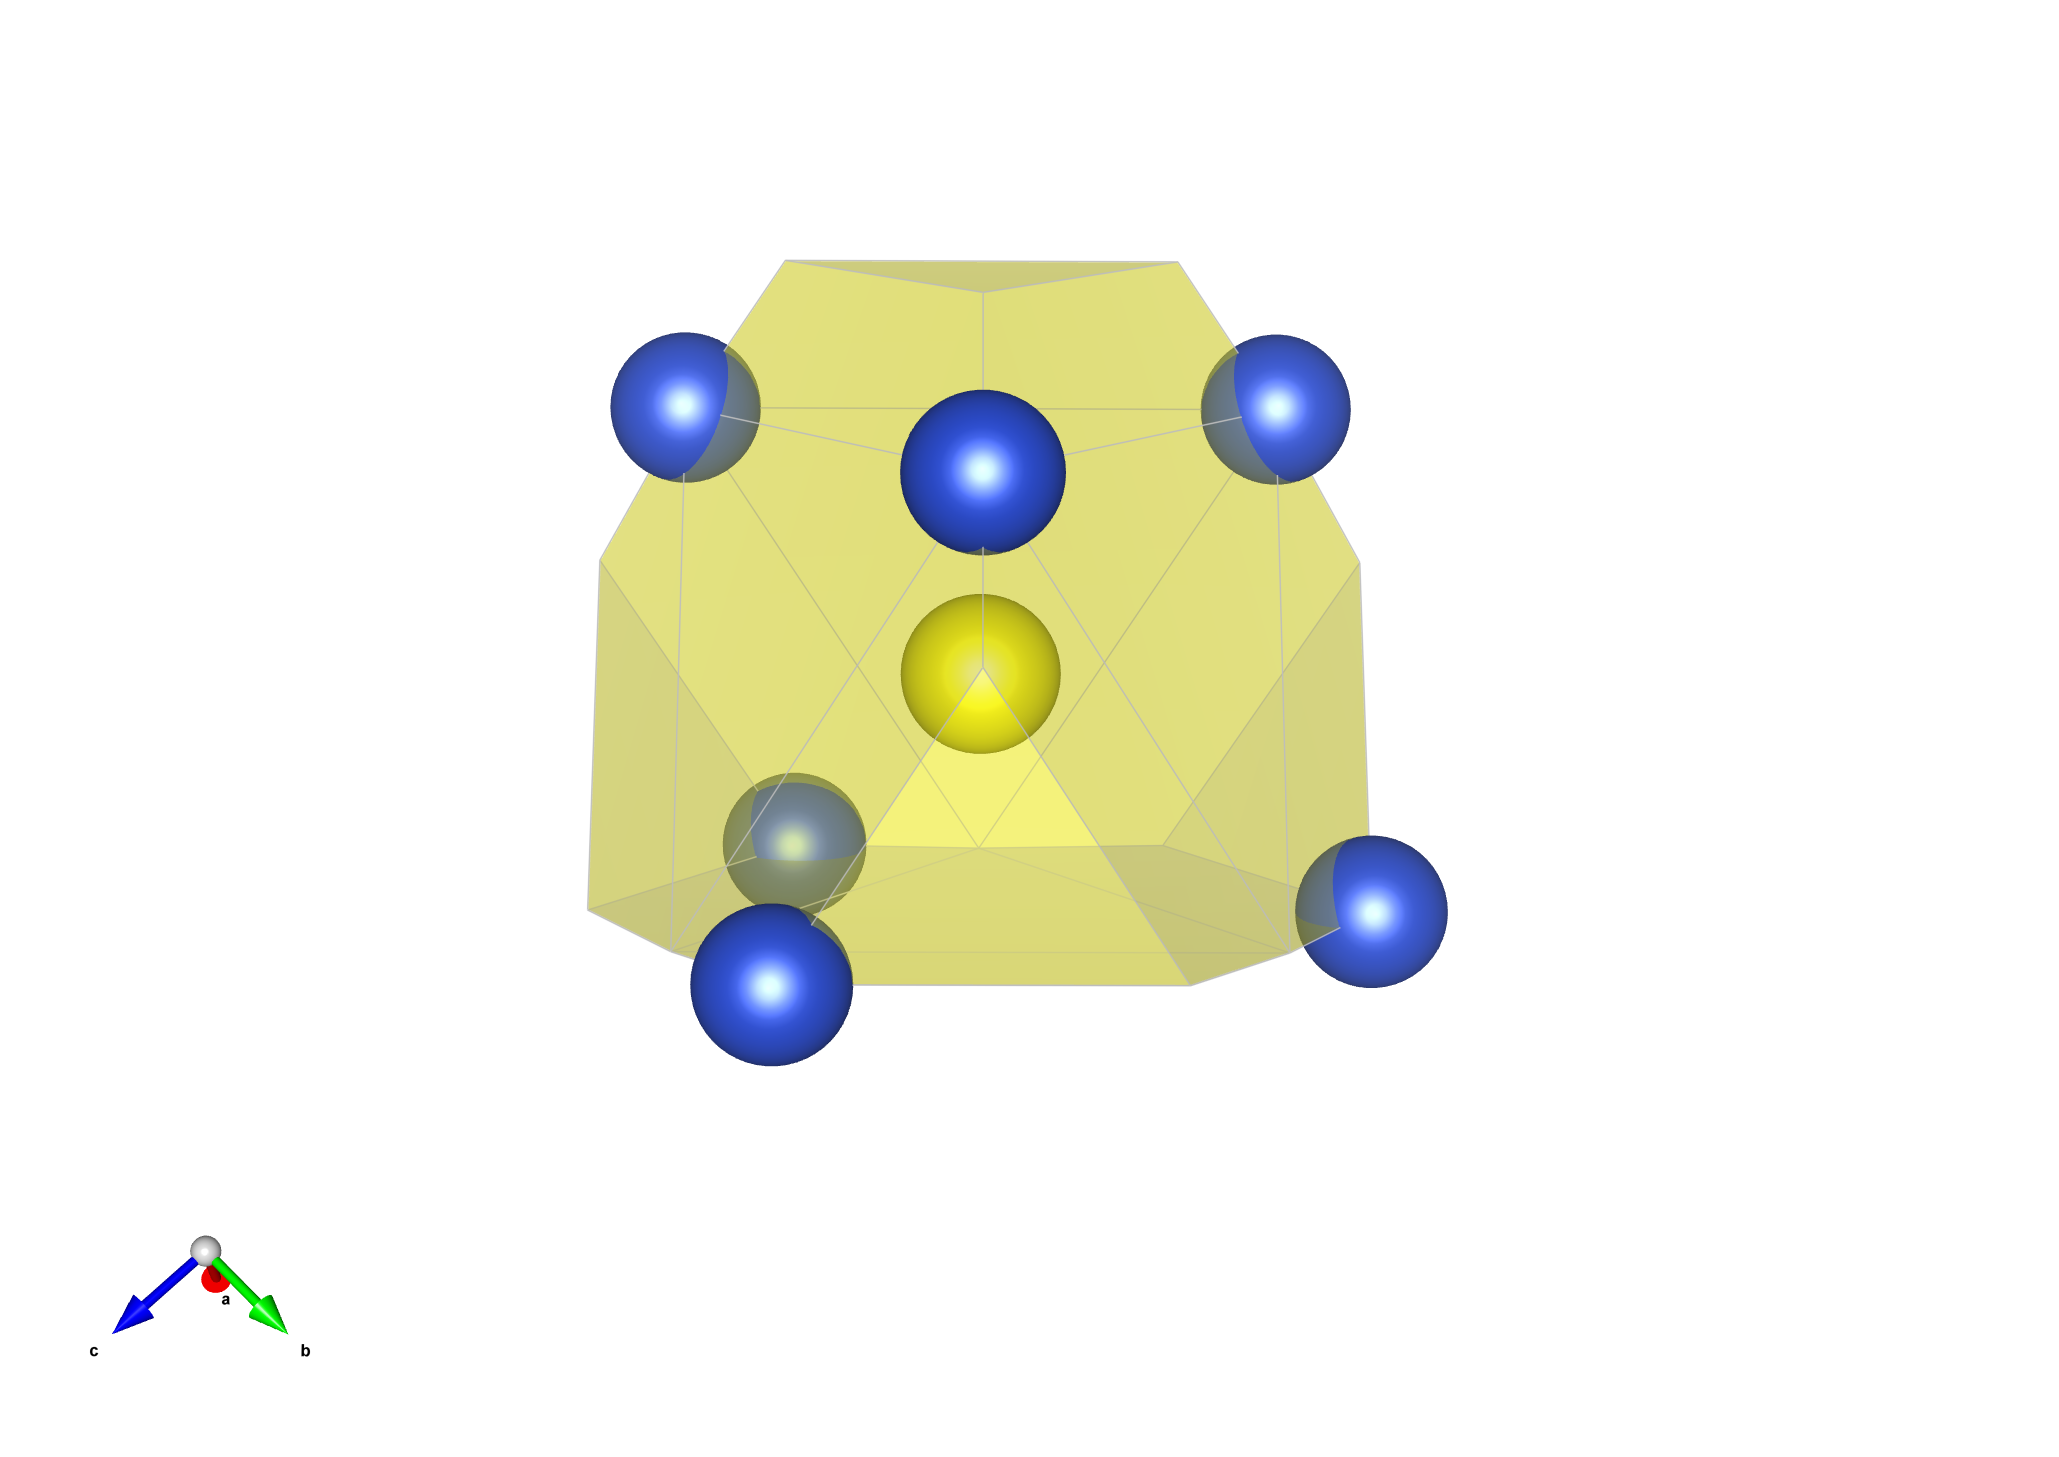
\includegraphics[width=0.9\linewidth]{var_1} \\ б)
  \end{minipage}
\vfill

  \begin{minipage}[ht]{0.45\linewidth}\centering
    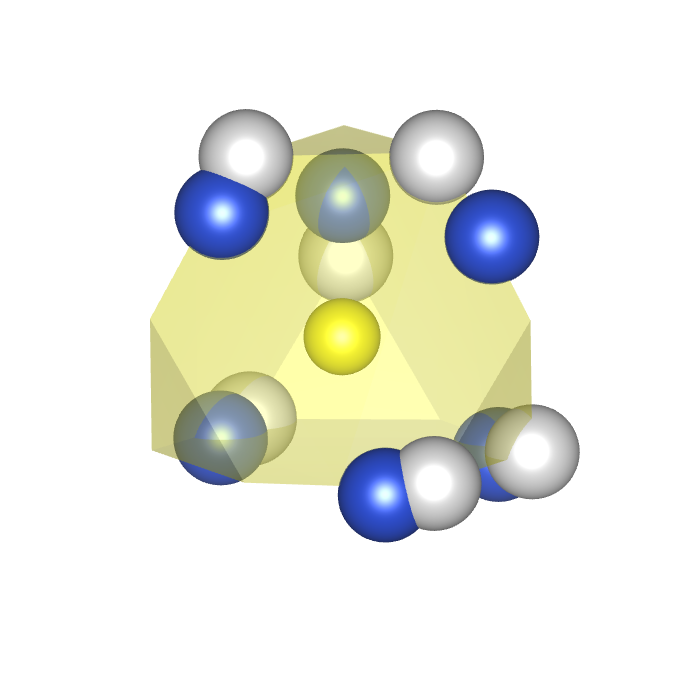
\includegraphics[width=0.9\linewidth]{var_2} \\ в)
  \end{minipage}
						\hfill
 \begin{minipage}[ht]{0.45\linewidth}\centering
    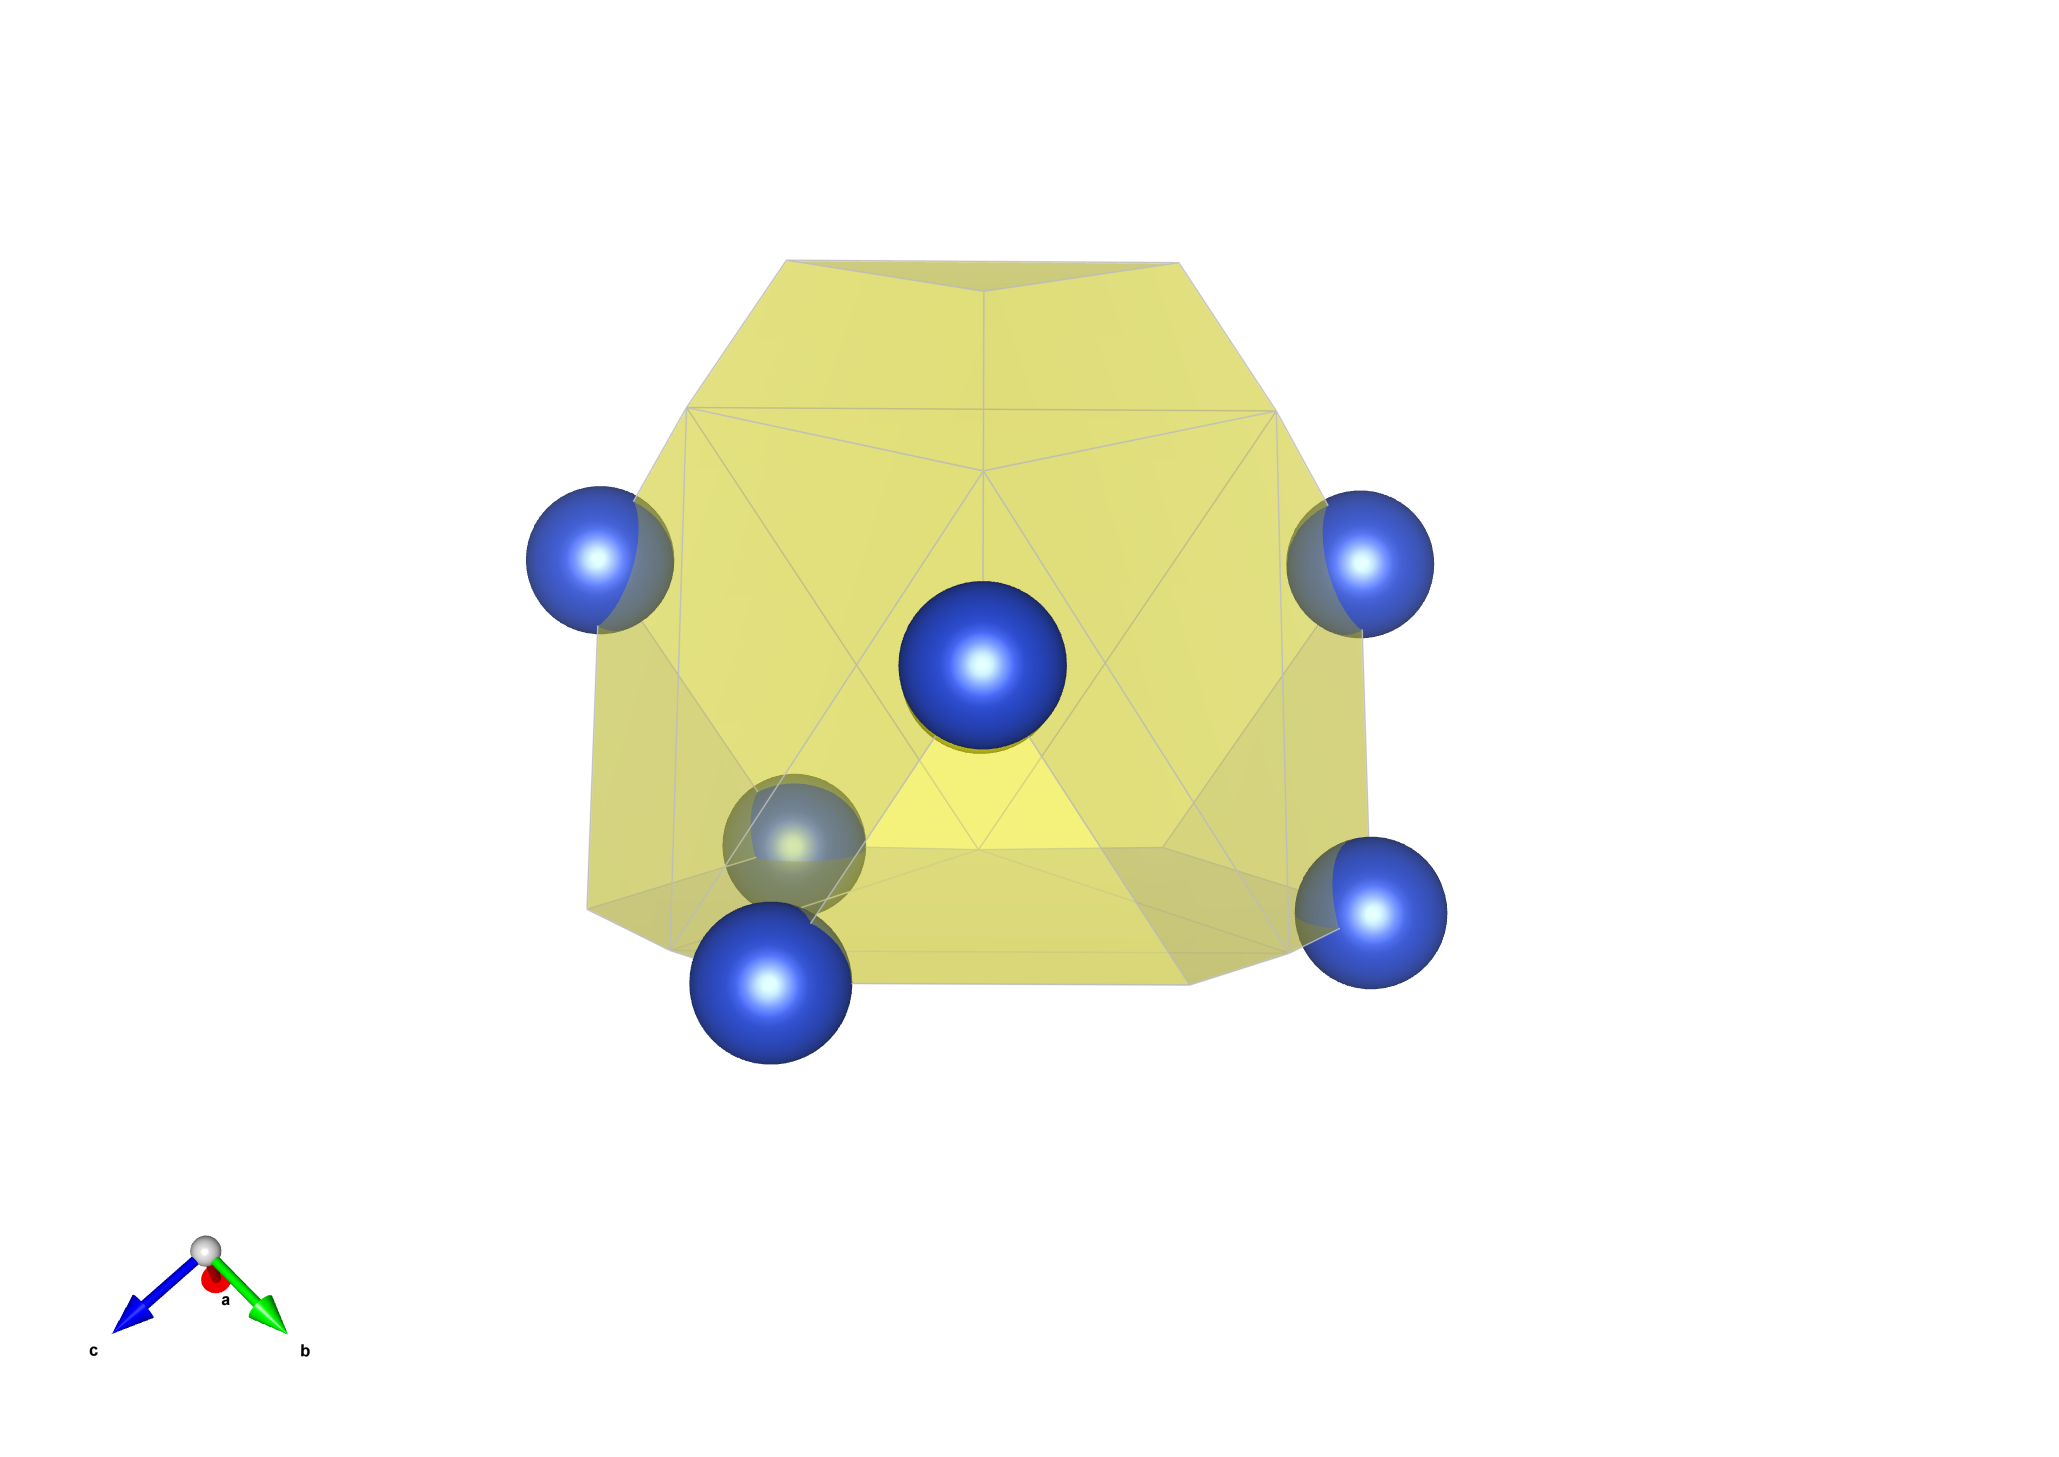
\includegraphics[width=0.9\linewidth]{var_3} \\ г)
  \end{minipage}
\vfill

  \begin{minipage}[ht]{0.45\linewidth}\centering
    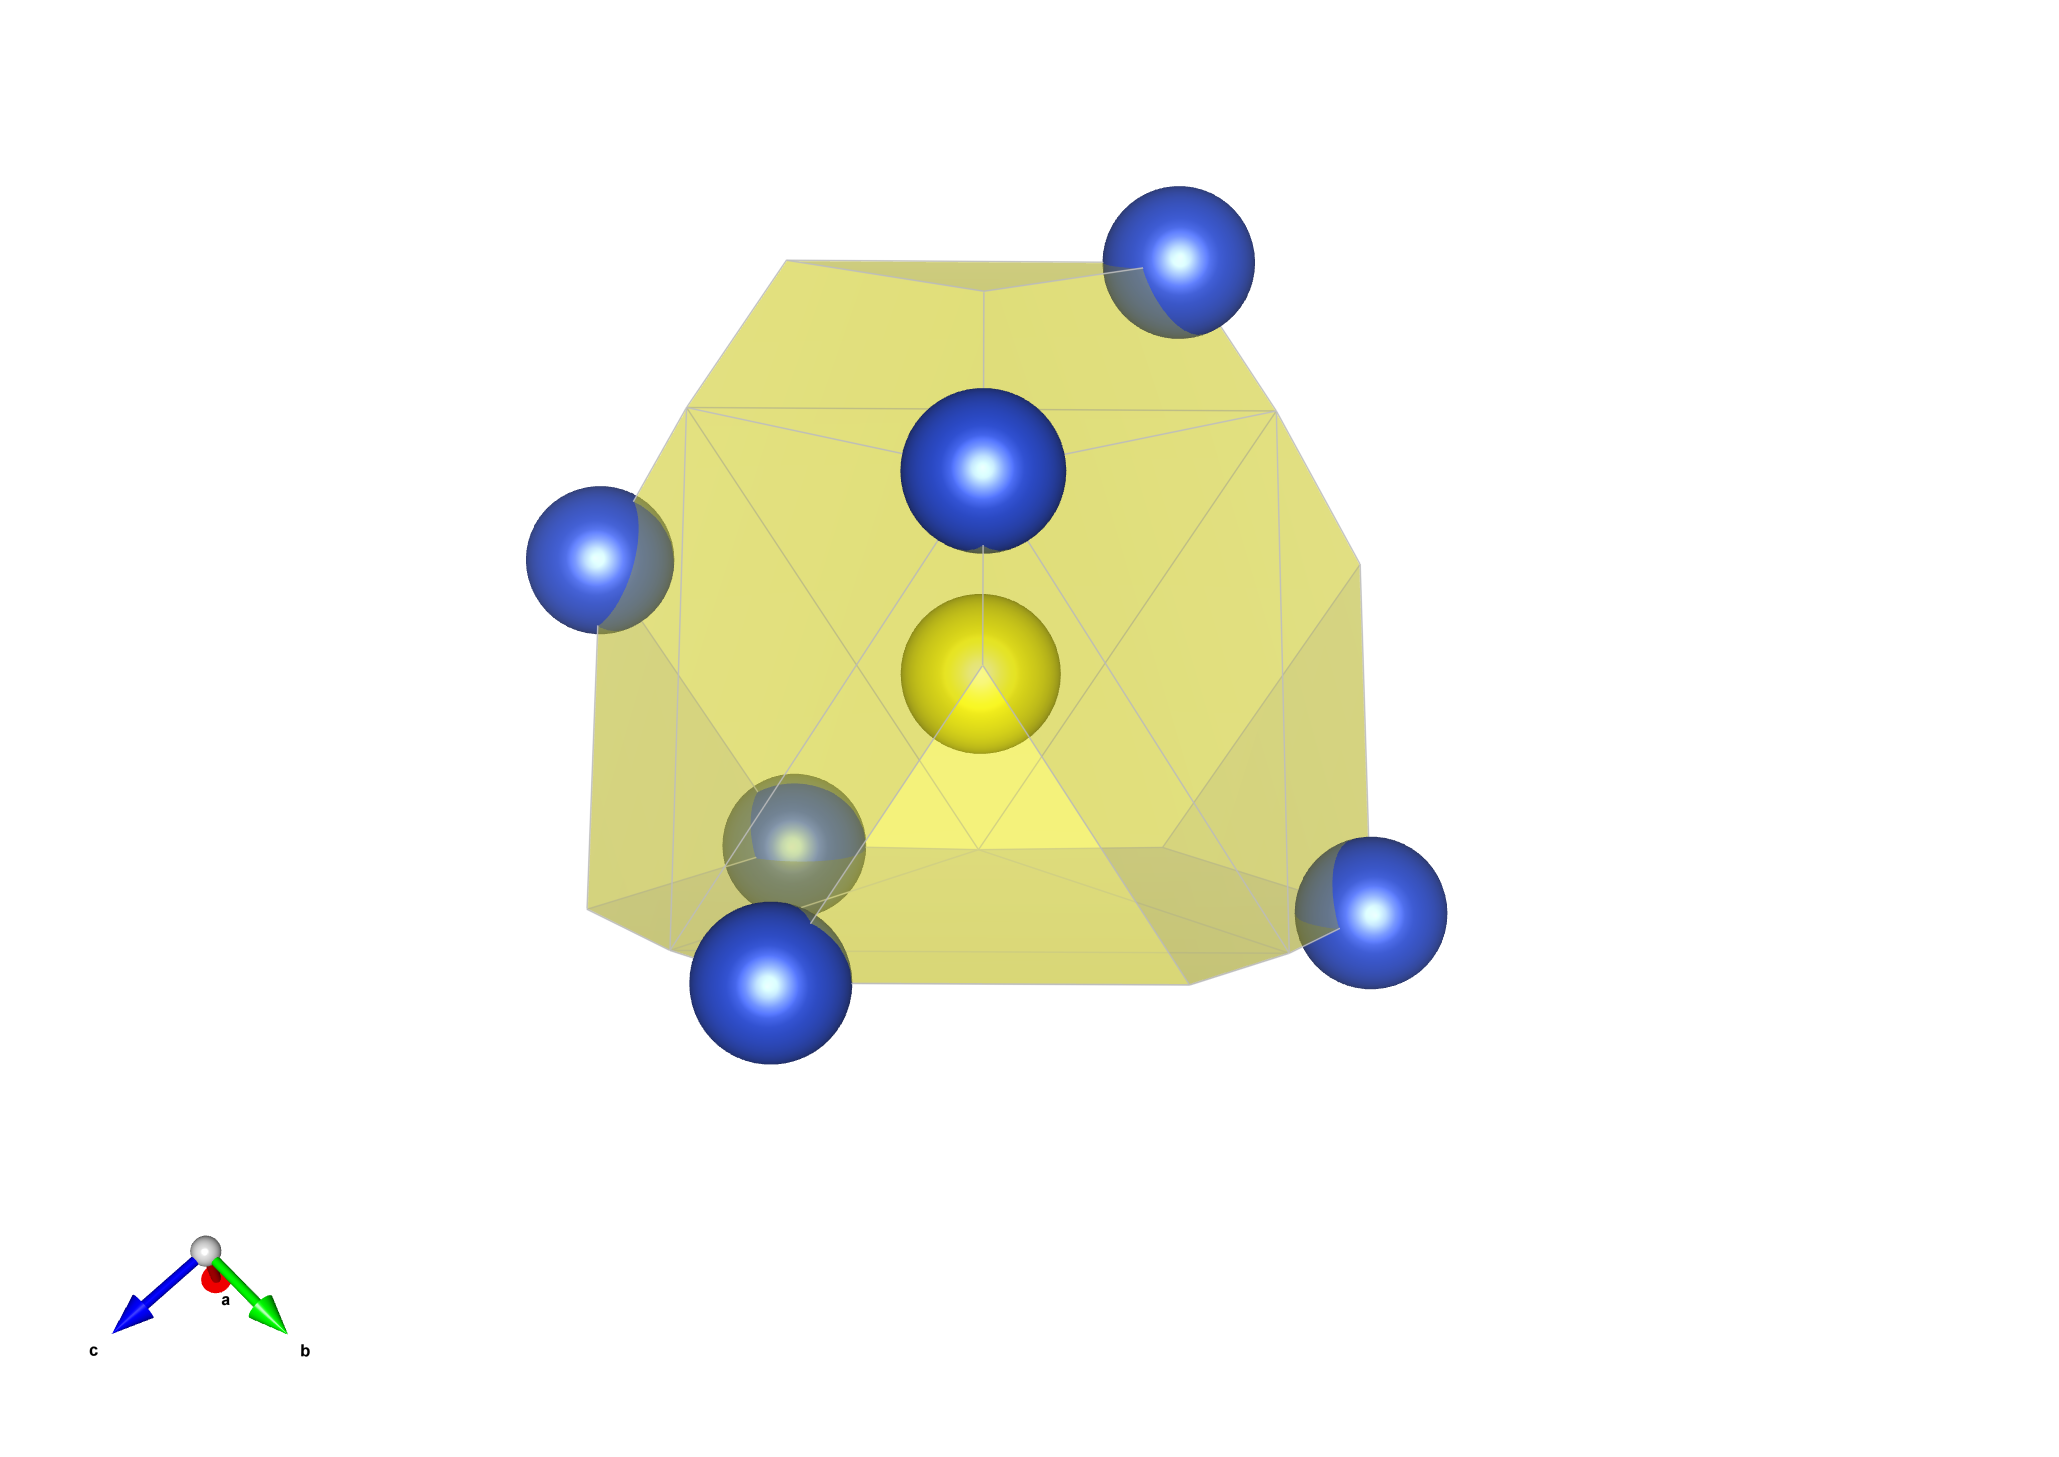
\includegraphics[width=0.9\linewidth]{var_4} \\ д)
  \end{minipage}
						\hfill
 \begin{minipage}[ht]{0.45\linewidth}\centering
    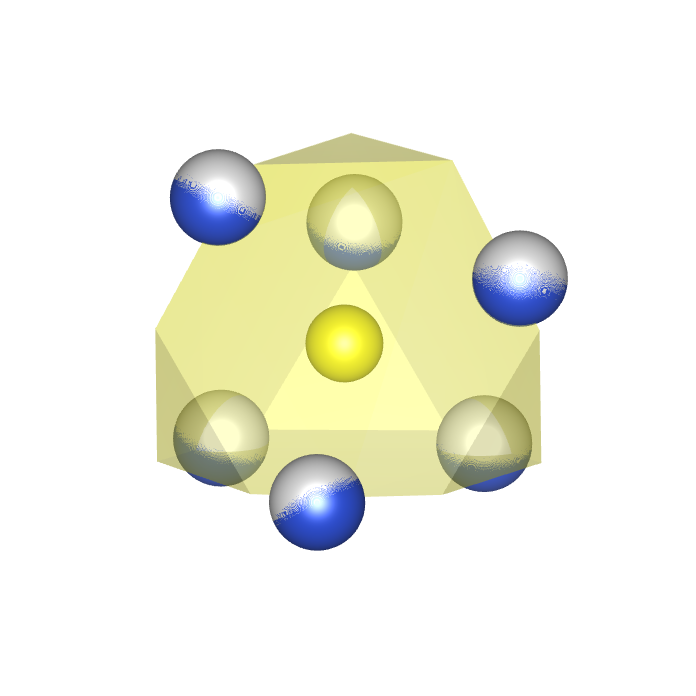
\includegraphics[width=0.9\linewidth]{var_5} \\ е)
  \end{minipage}
      \caption[Изображения лавесовских полиэдров синтетического теннантита Cu\textsubscript{12}As\textsubscript{4}S\textsubscript{13}, для которых рассчитывалась энергия элементарной ячейки. Варианты с 0 по 5 включительно]{Изображения лавесовских полиэдров синтетического теннантита Cu\textsubscript{12}As\textsubscript{4}S\textsubscript{13}, для которых рассчитывалась энергия элементарной ячейки. Варианты с 0 по 5 включительно}
    \label{img:laves1}
\end{figure}

\begin{figure}[p!]
  \begin{minipage}[ht]{0.45\linewidth}\centering
    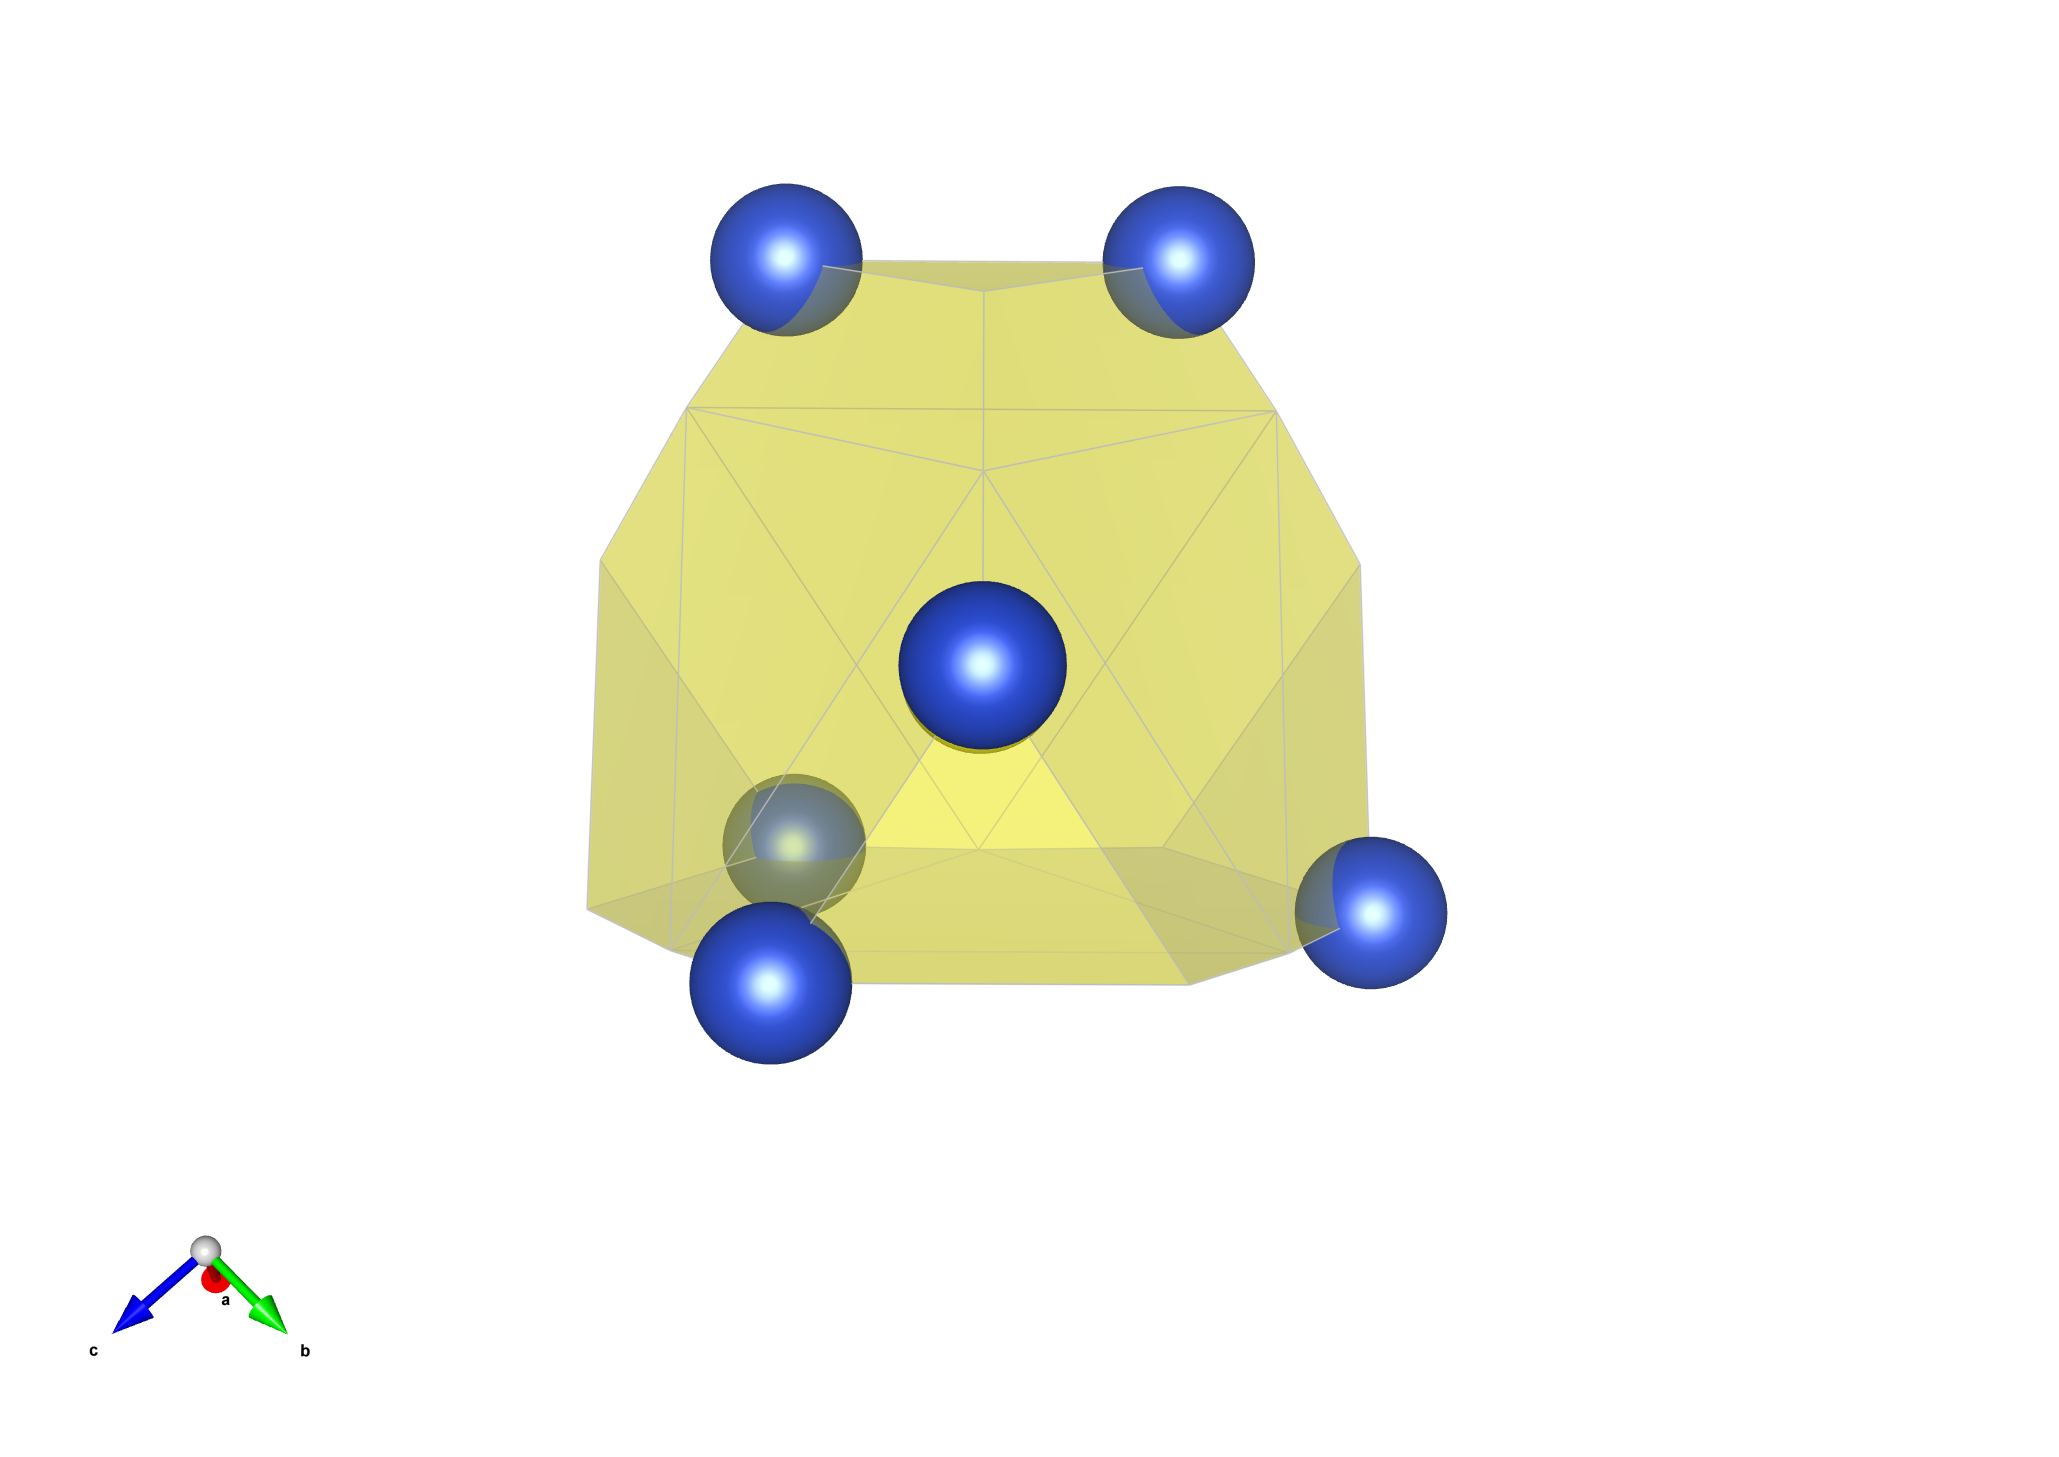
\includegraphics[width=0.9\linewidth]{var_6} \\ а)
  \end{minipage}
						\hfill
 \begin{minipage}[ht]{0.45\linewidth}\centering
    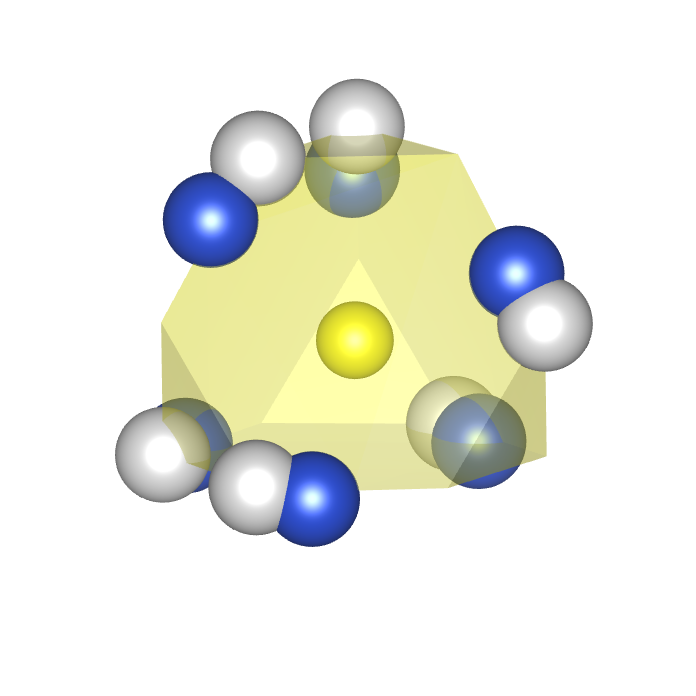
\includegraphics[width=0.9\linewidth]{var_7} \\ б)
  \end{minipage}
\vfill

  \begin{minipage}[ht]{0.45\linewidth}\centering
    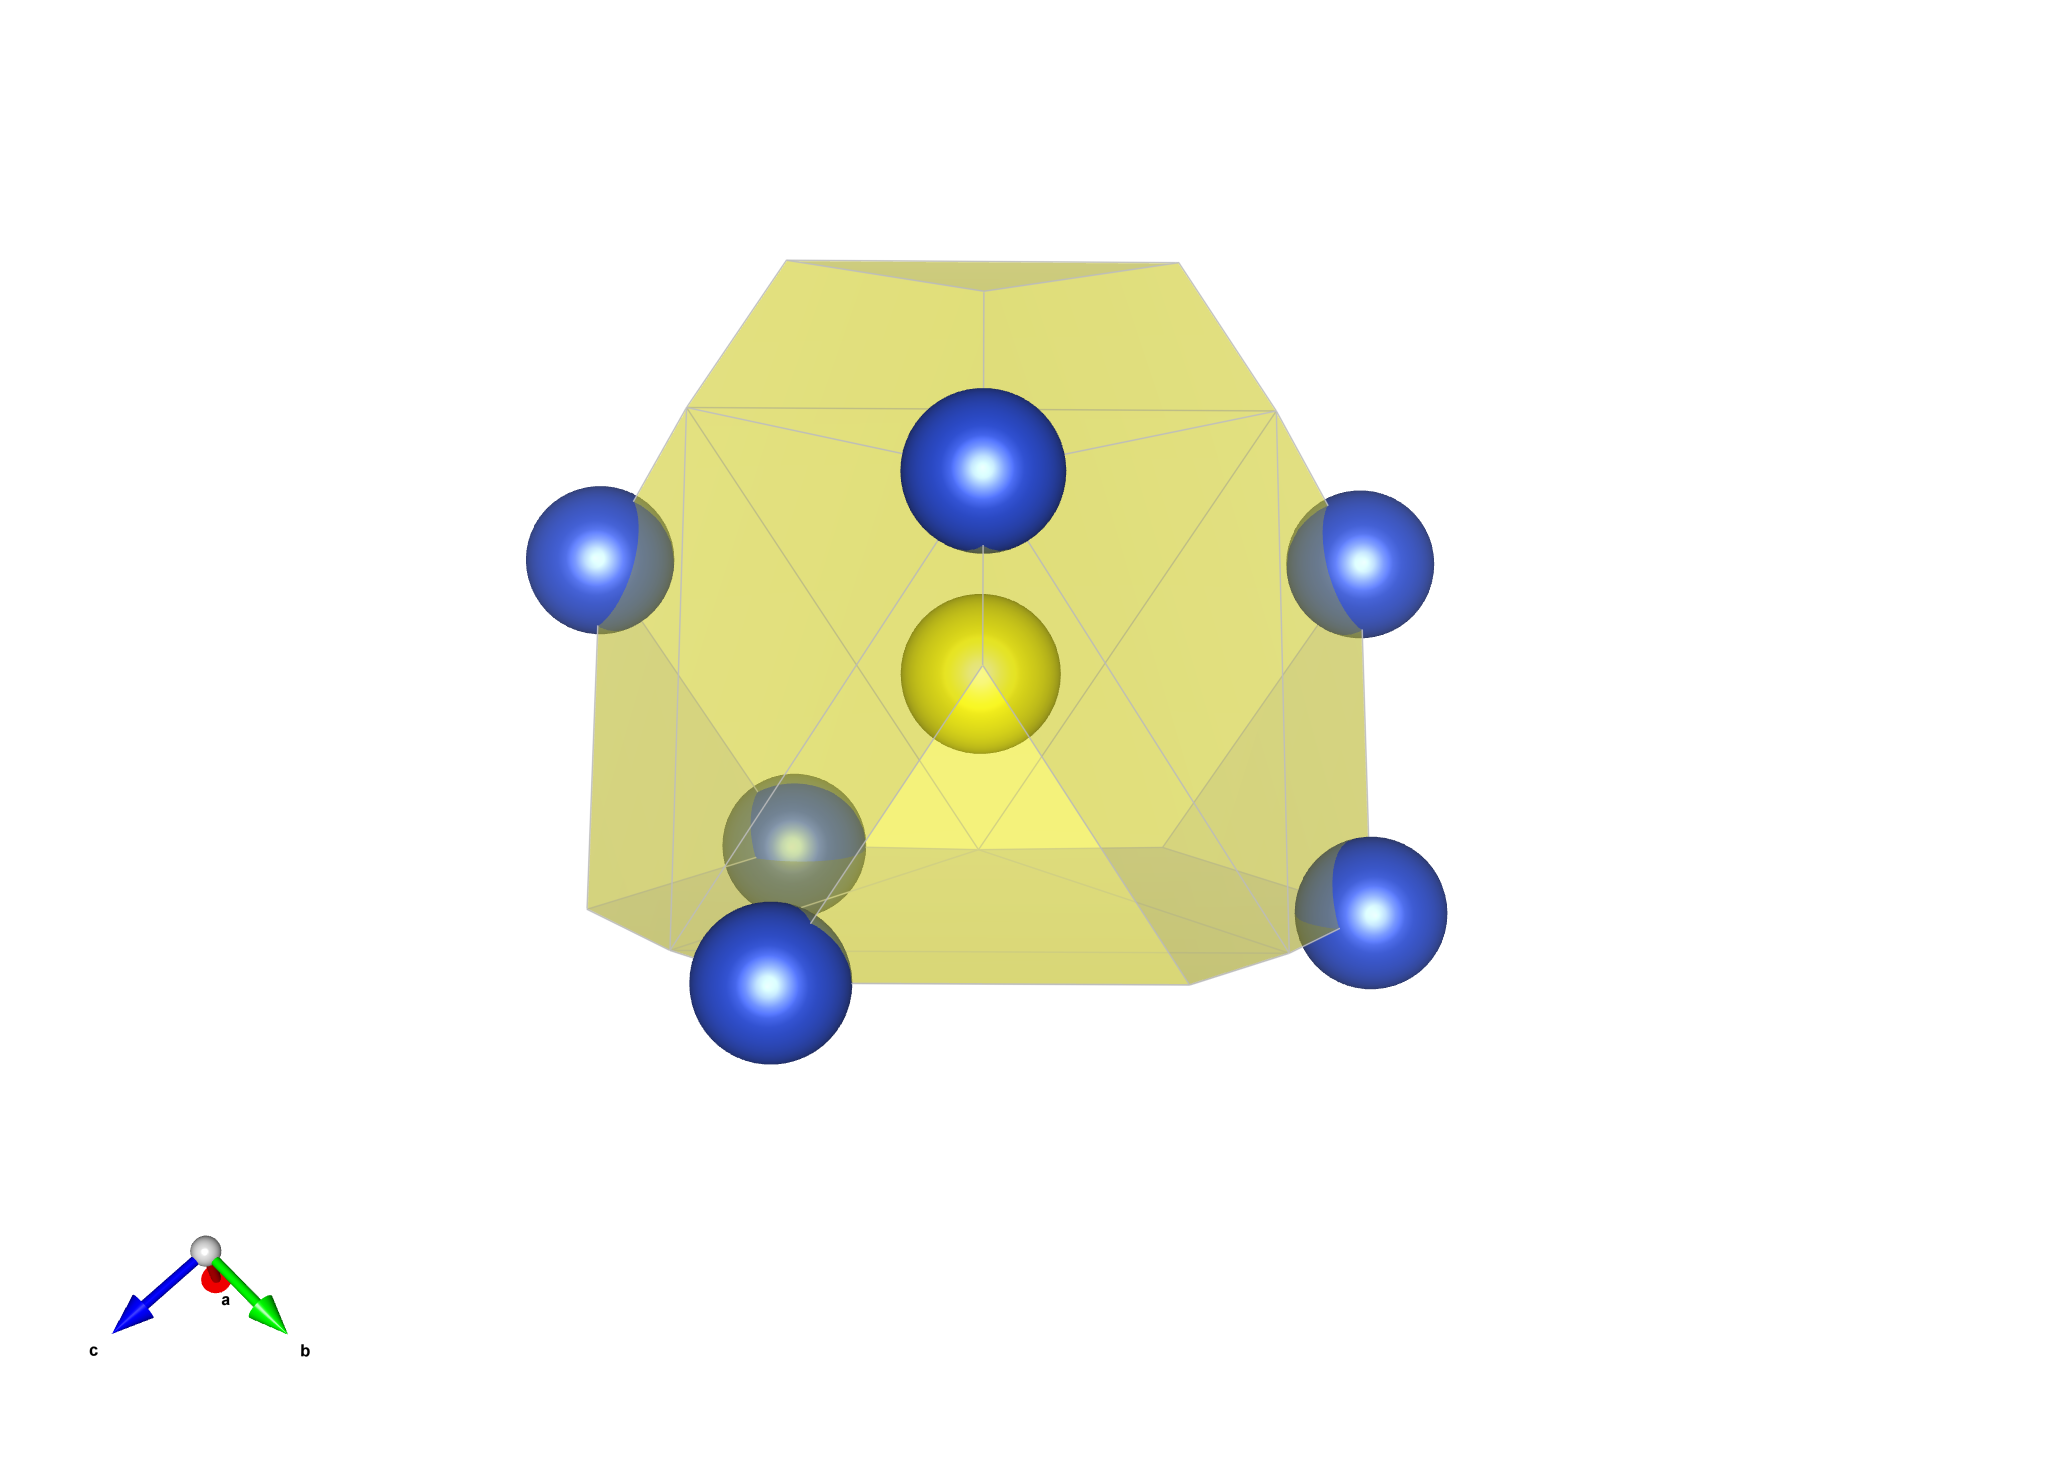
\includegraphics[width=0.9\linewidth]{var_8} \\ в)
  \end{minipage}
						\hfill
 \begin{minipage}[ht]{0.45\linewidth}\centering
    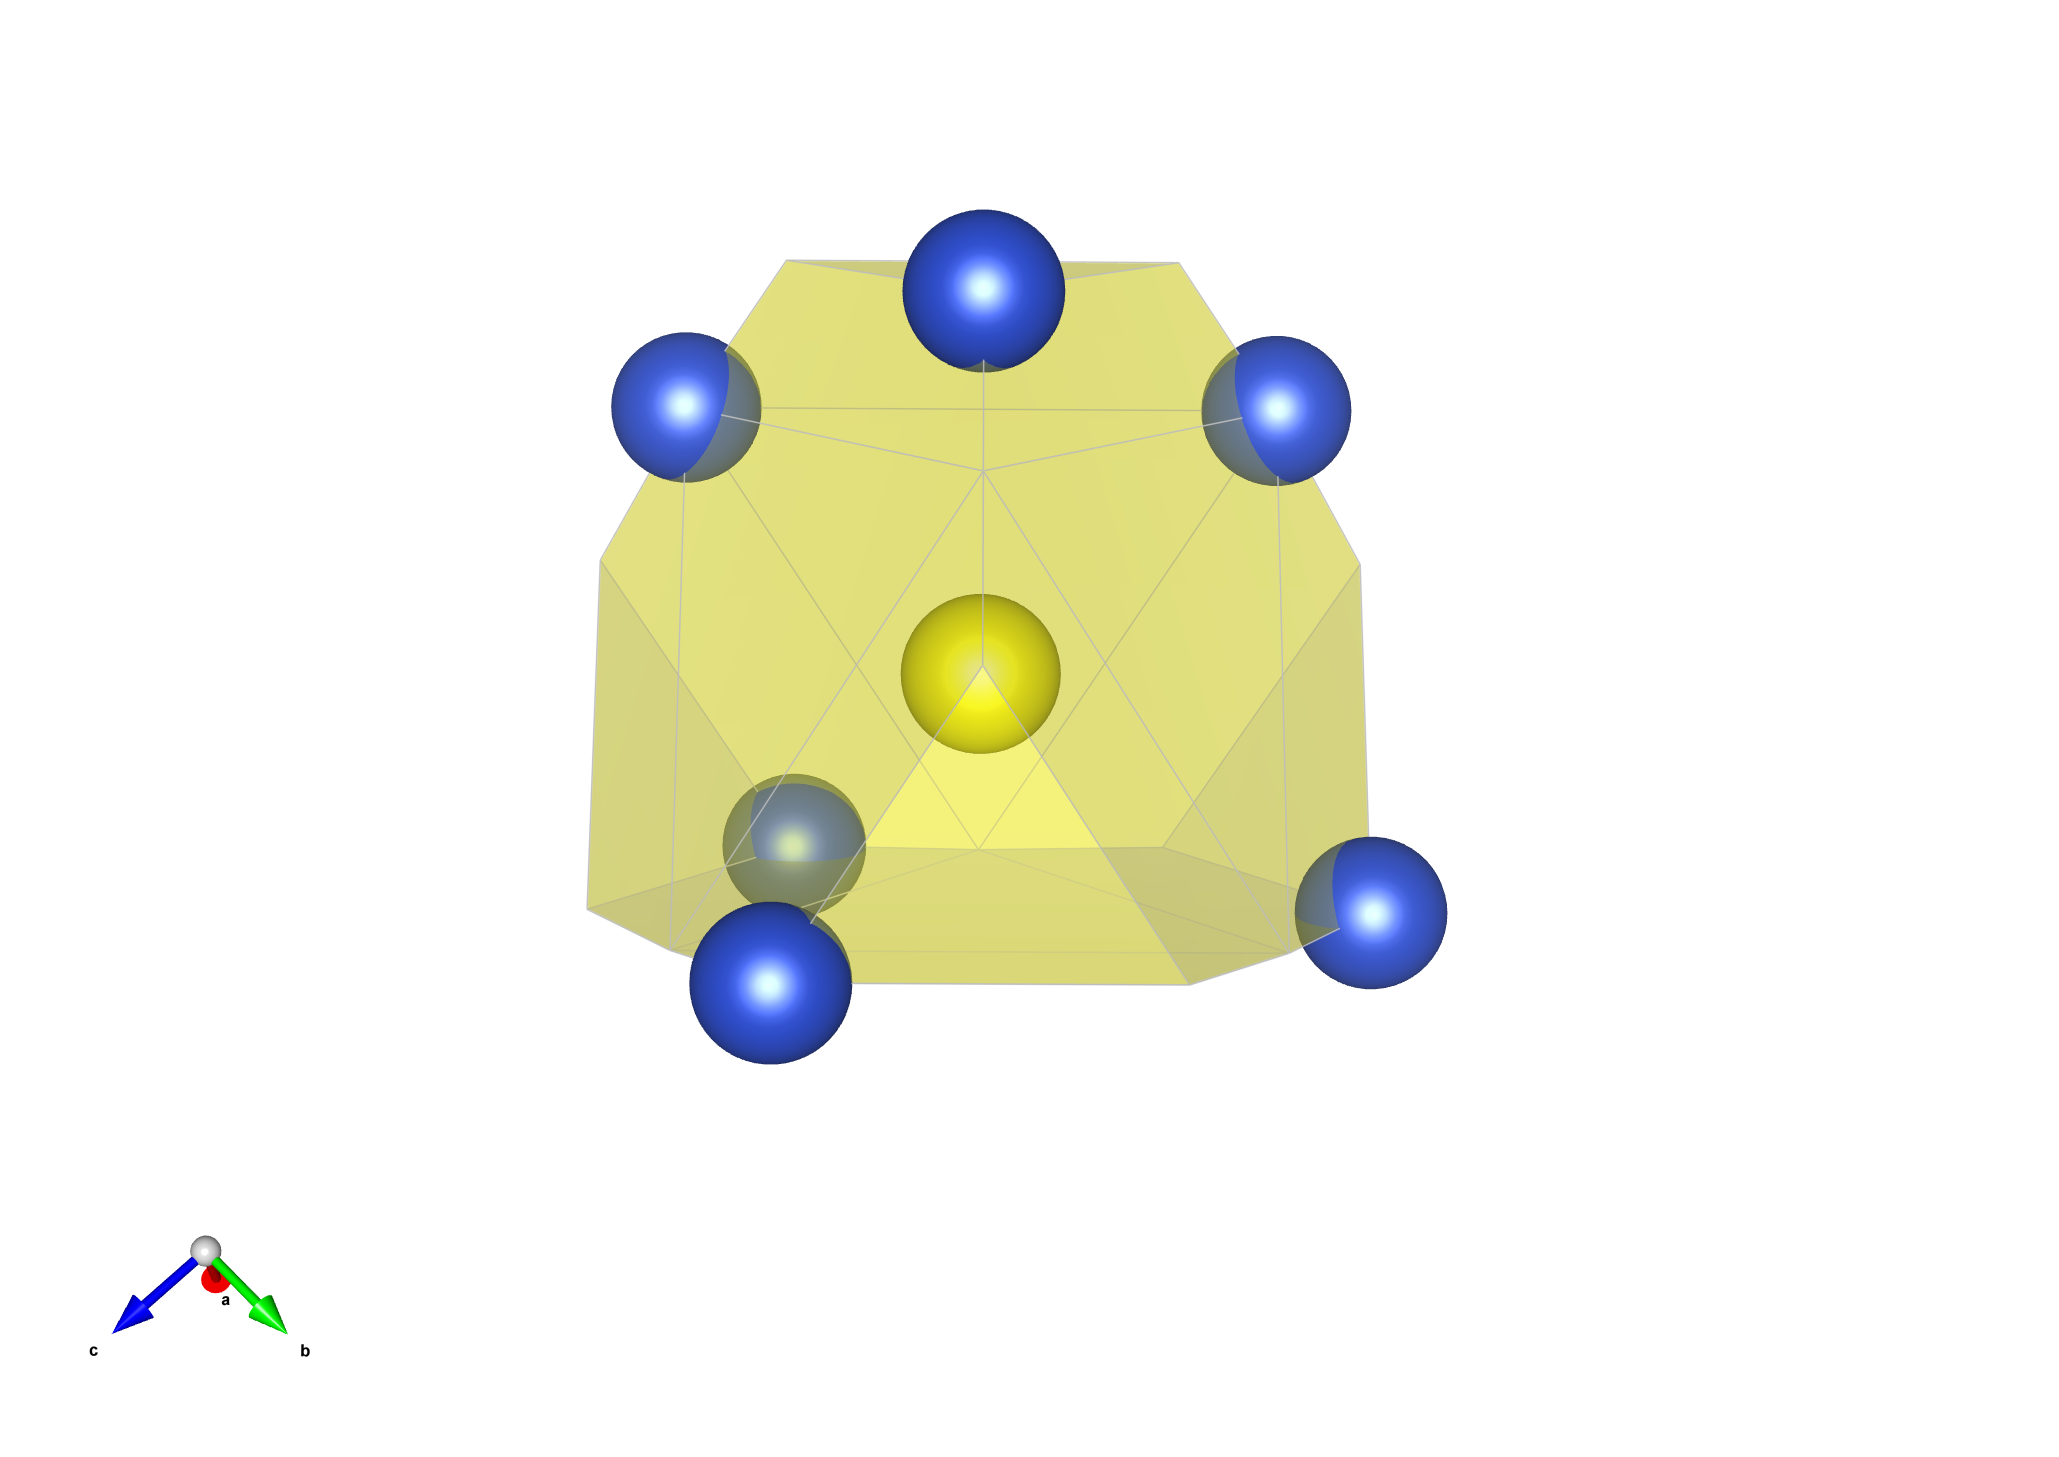
\includegraphics[width=0.9\linewidth]{var_9} \\ г)
  \end{minipage}
\vfill

  \begin{minipage}[ht]{0.45\linewidth}\centering
    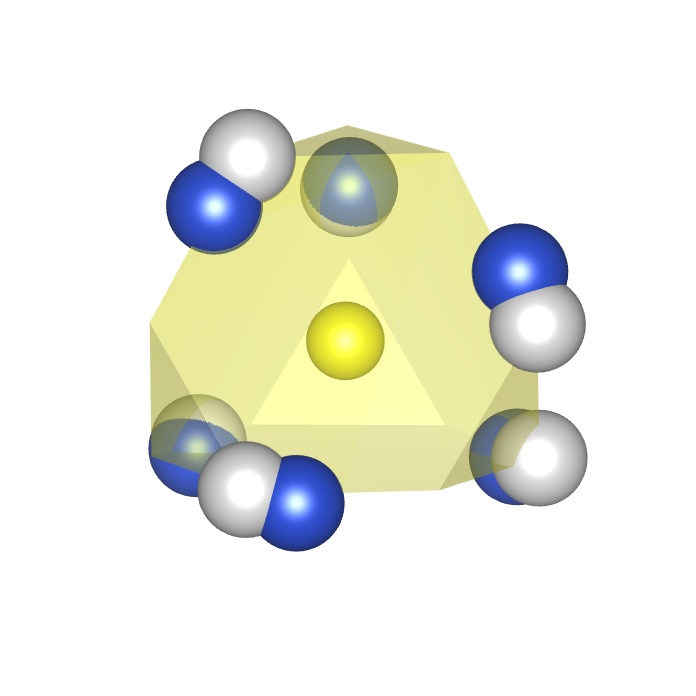
\includegraphics[width=0.9\linewidth]{var_10} \\ д)
  \end{minipage}
						\hfill
 \begin{minipage}[ht]{0.45\linewidth}\centering
    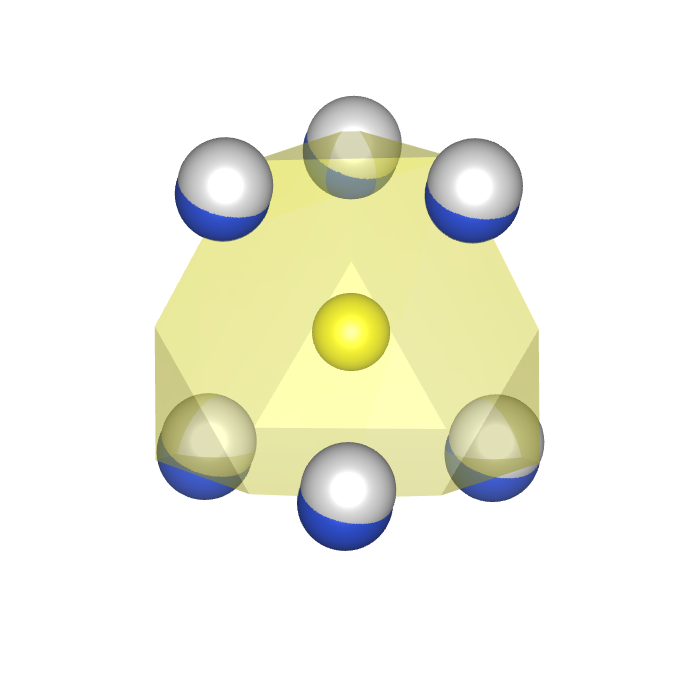
\includegraphics[width=0.9\linewidth]{var_11} \\ е)
  \end{minipage}
      \caption[Изображения лавесовских полиэдров синтетического теннантита Cu\textsubscript{12}As\textsubscript{4}S\textsubscript{13}, для которых рассчитывалась энергия элементарной ячейки. Варианты с 6 по 11 включительно]{Изображения лавесовских полиэдров синтетического теннантита Cu\textsubscript{12}As\textsubscript{4}S\textsubscript{13}, для которых рассчитывалась энергия элементарной ячейки. Варианты с 6 по 11 включительно}
    \label{img:laves2}
\end{figure}



\begin{figure}[p!]
  \begin{minipage}[ht]{0.45\linewidth}\centering
    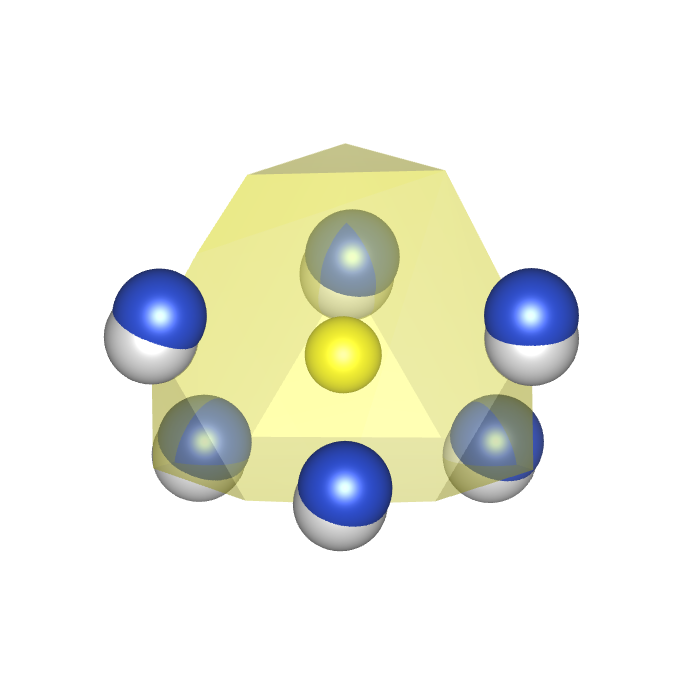
\includegraphics[width=0.9\linewidth]{var_12} \\ а)
  \end{minipage}
\hfill
 \begin{minipage}[ht]{0.45\linewidth}\centering
    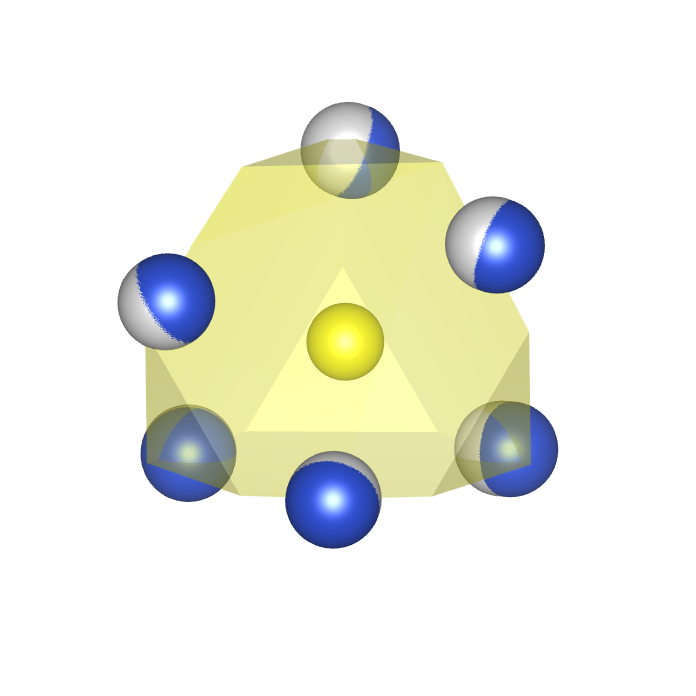
\includegraphics[width=0.9\linewidth]{var_13} \\ б)
  \end{minipage}
\vfill
  \begin{minipage}[ht]{0.45\linewidth}\centering
    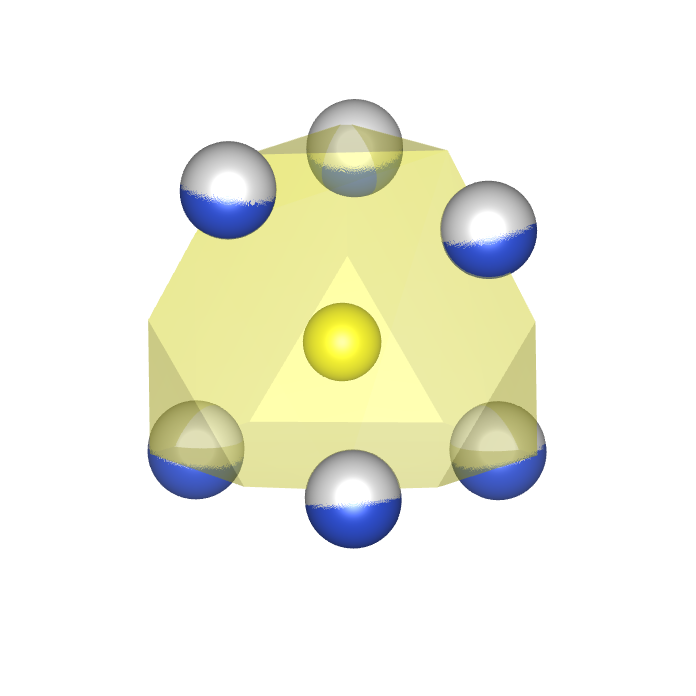
\includegraphics[width=0.9\linewidth]{var_14} \\ в)
  \end{minipage}
	\hfill
 \begin{minipage}[ht]{0.45\linewidth}\centering
    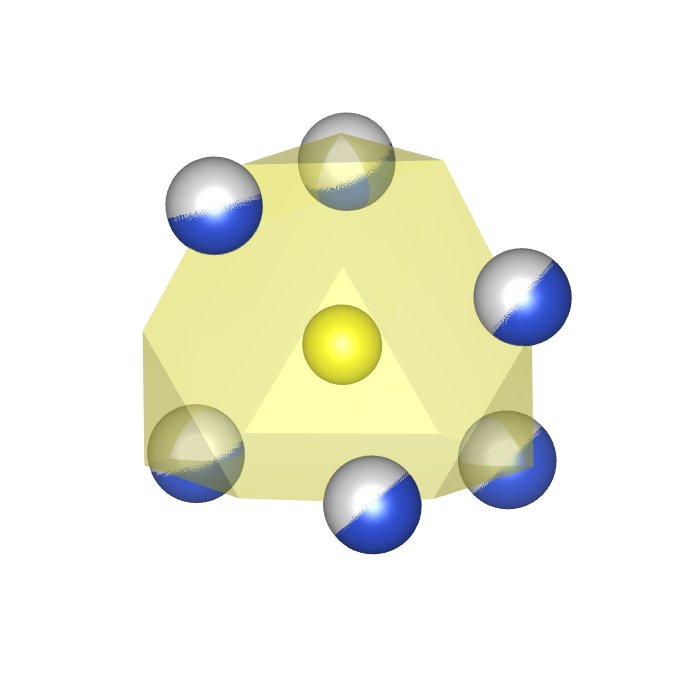
\includegraphics[width=0.9\linewidth]{var_15} \\ г)
  \end{minipage}
\vfill

  \begin{minipage}[ht]{0.45\linewidth}\centering

  \end{minipage}
						\hfill
 \begin{minipage}[ht]{0.45\linewidth}\centering

  \end{minipage}
      \caption[Изображения лавесовских полиэдров синтетического теннантита Cu\textsubscript{12}As\textsubscript{4}S\textsubscript{13}, для которых рассчитывалась энергия элементарной ячейки. Варианты с 12 по 15 включительно]{Изображения лавесовских полиэдров синтетического теннантита Cu\textsubscript{12}As\textsubscript{4}S\textsubscript{13}, для которых рассчитывалась энергия элементарной ячейки. Варианты с 6 по 11 включительно}
    \label{img:laves3}
\end{figure}


\begin{figure}[p!]
  \begin{minipage}[ht]{0.45\linewidth}\centering
    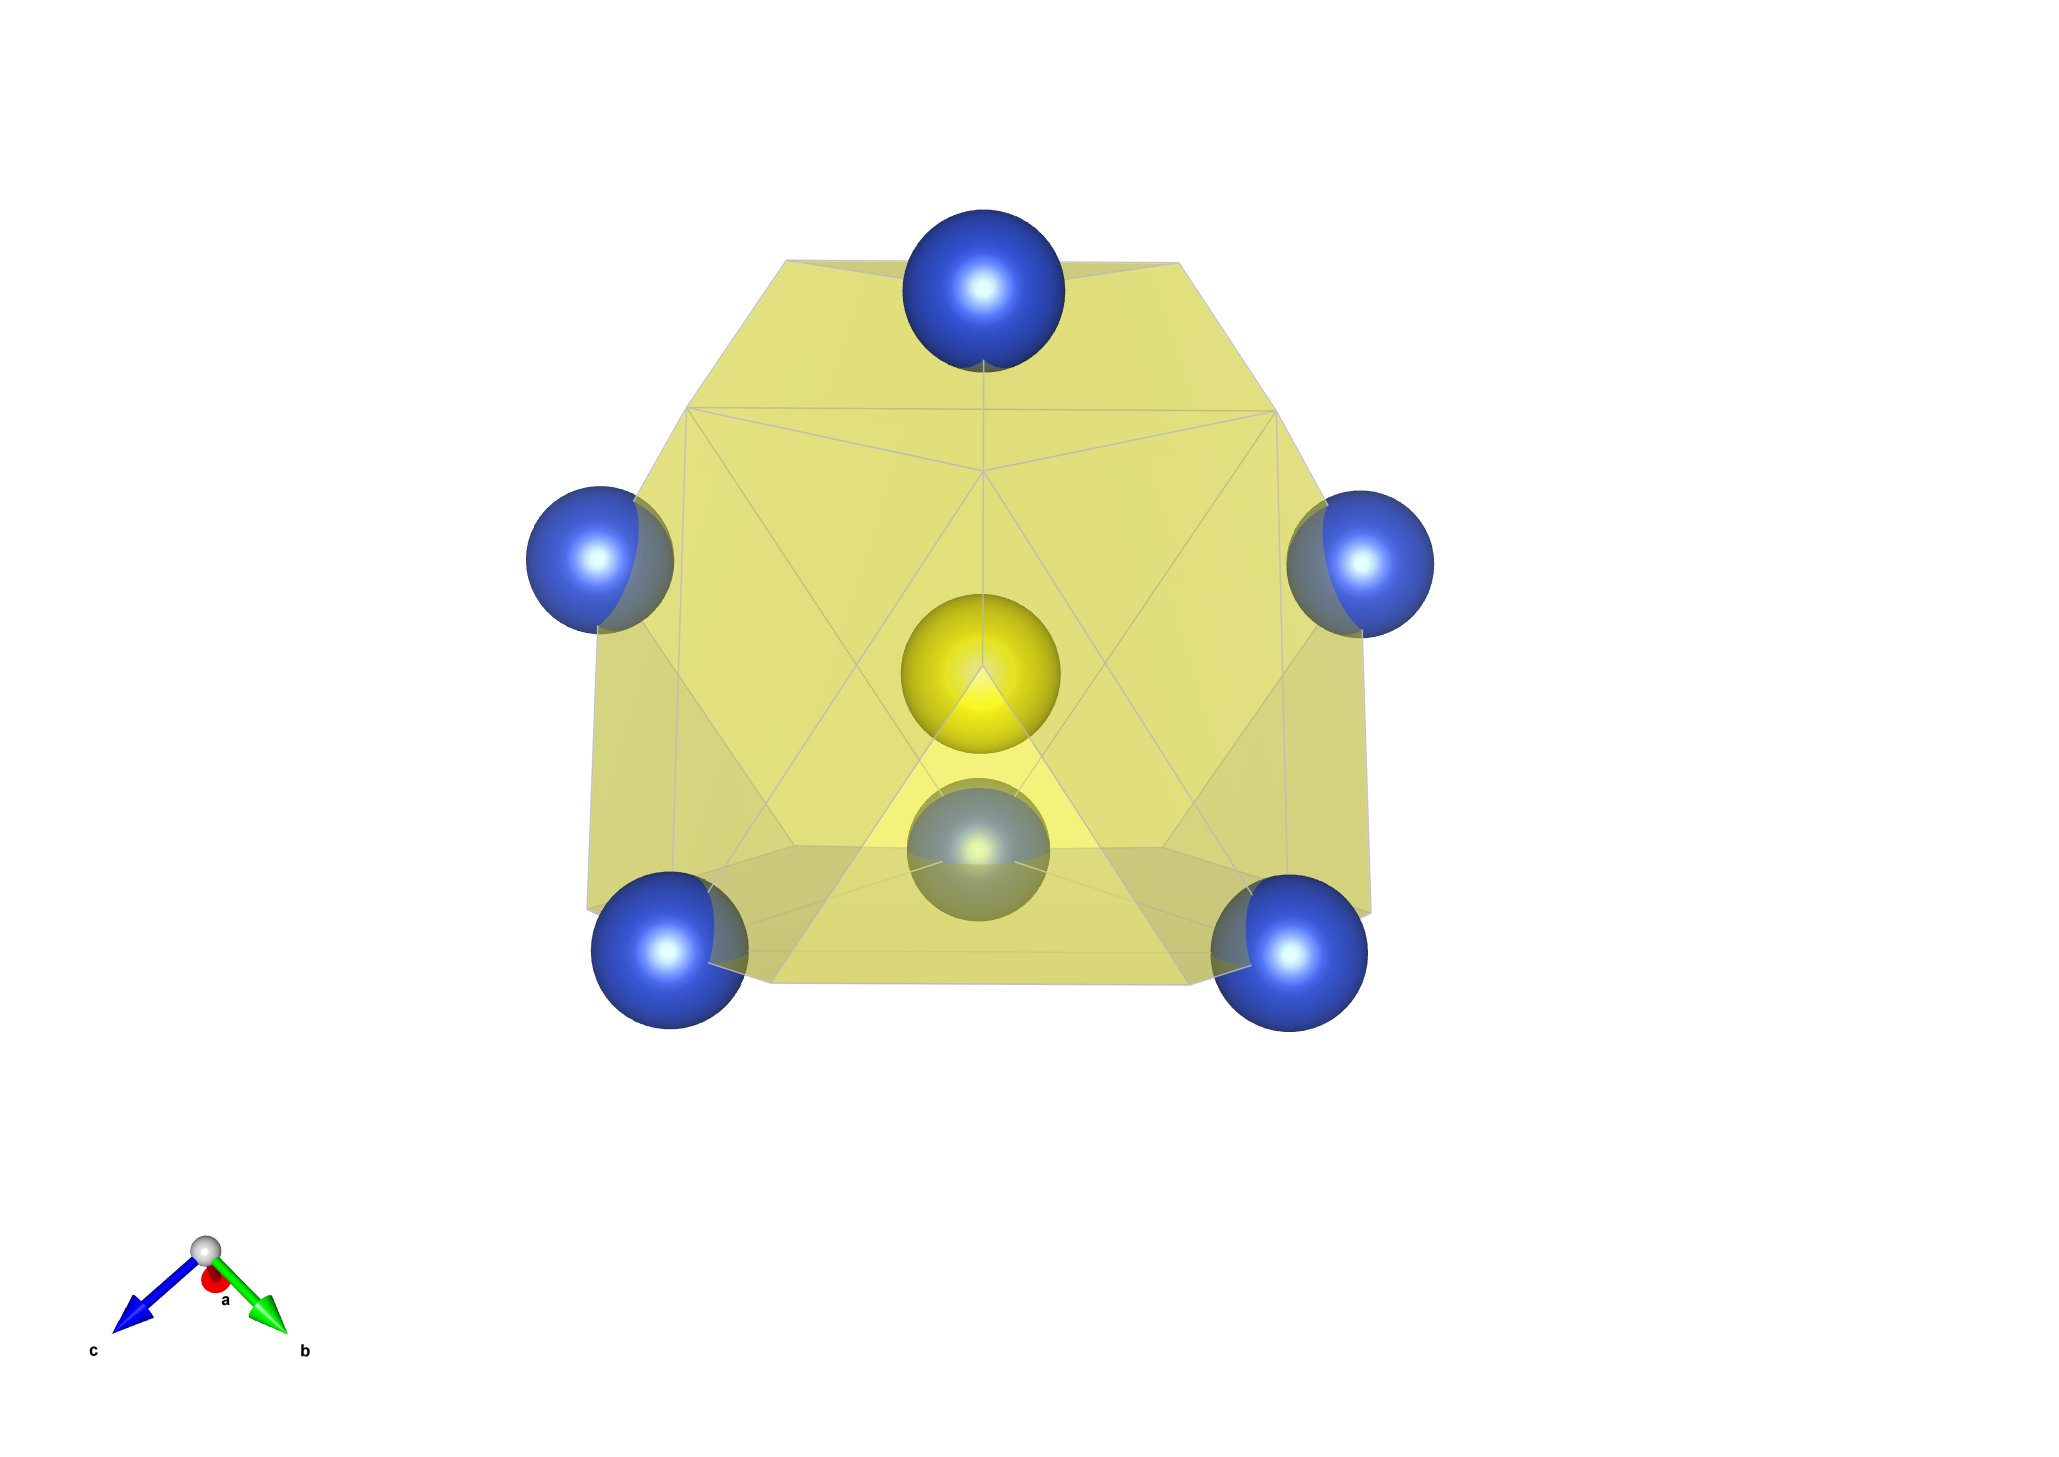
\includegraphics[width=0.9\linewidth]{var_16} \\ а)
  \end{minipage}
						\hfill
 \begin{minipage}[ht]{0.45\linewidth}\centering
    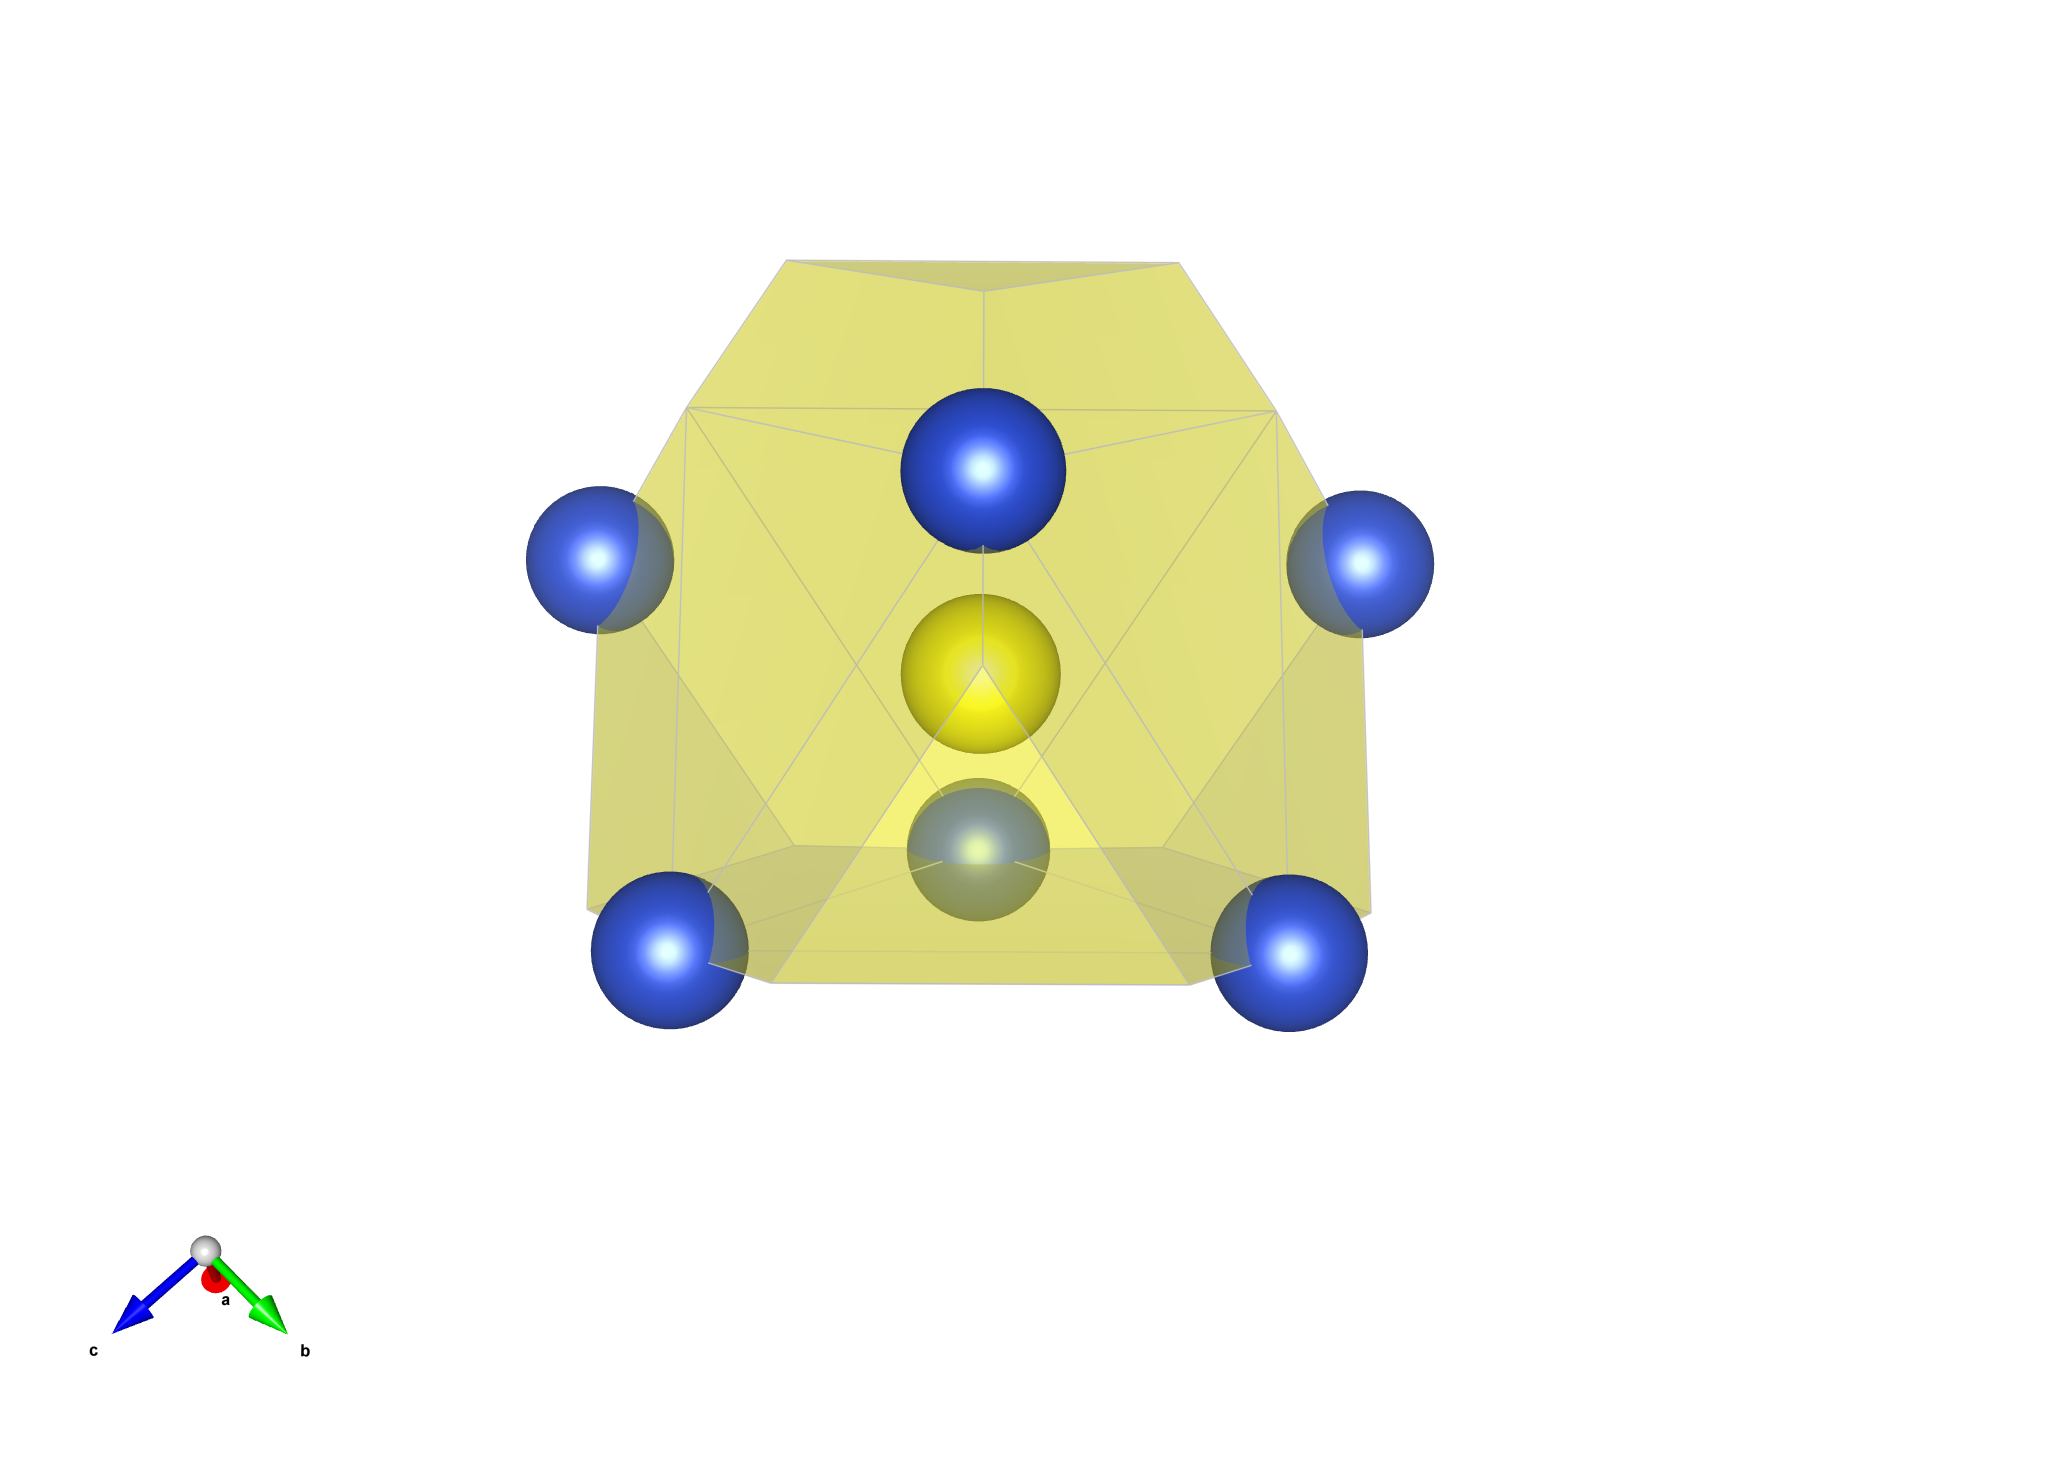
\includegraphics[width=0.9\linewidth]{var_17} \\ б)
  \end{minipage}
\vfill

  \begin{minipage}[ht]{0.45\linewidth}\centering
    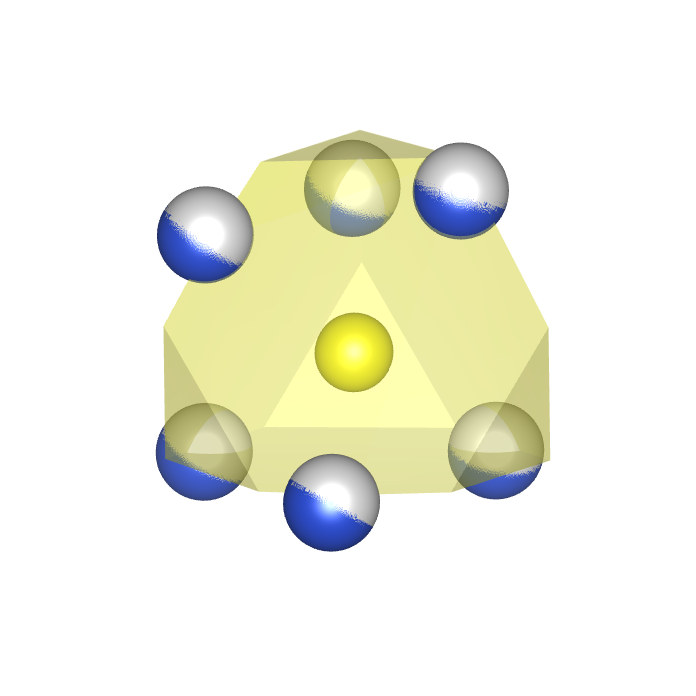
\includegraphics[width=0.9\linewidth]{var_18} \\ в)
  \end{minipage}
						\hfill
 \begin{minipage}[ht]{0.45\linewidth}\centering
    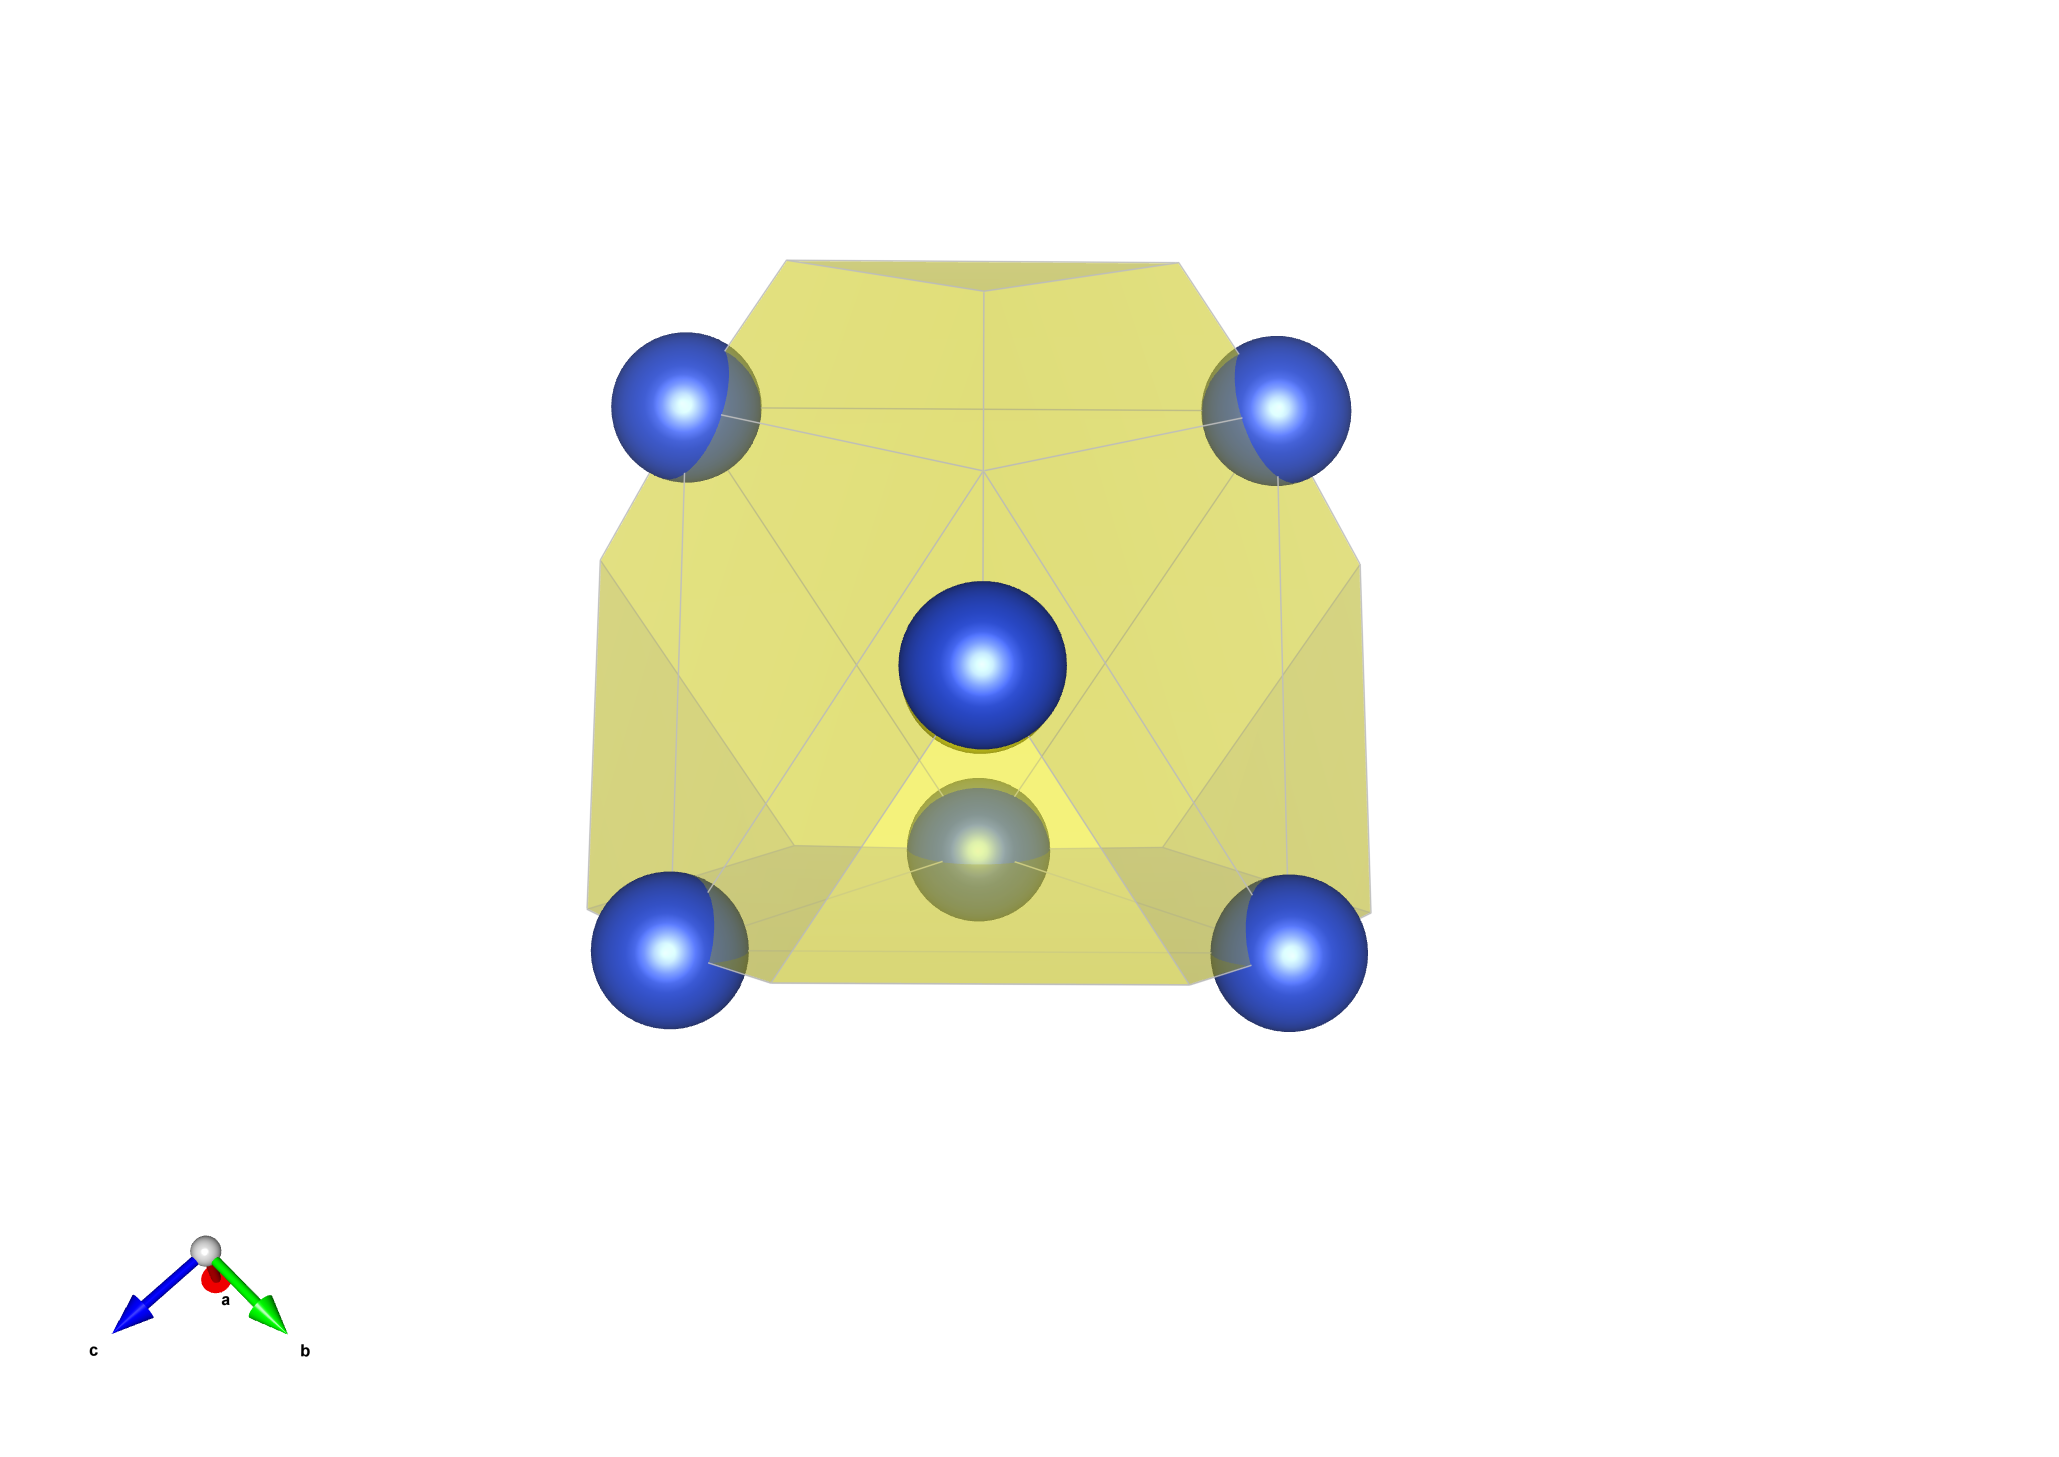
\includegraphics[width=0.9\linewidth]{var_19} \\ г)
  \end{minipage}
\vfill

  \begin{minipage}[ht]{0.45\linewidth}\centering

  \end{minipage}
						\hfill
 \begin{minipage}[ht]{0.45\linewidth}\centering

  \end{minipage}
      \caption[Изображения лавесовских полиэдров синтетического теннантита Cu\textsubscript{12}As\textsubscript{4}S\textsubscript{13}, для которых рассчитывалась энергия элементарной ячейки. Варианты с 16 по 19 включительно]{Изображения лавесовских полиэдров синтетического теннантита Cu\textsubscript{12}As\textsubscript{4}S\textsubscript{13}, для которых рассчитывалась энергия элементарной ячейки. Варианты с 16 по 19 включительно}
    \label{img:laves4}
\end{figure}



\newpage

\clearpage

\section{Особенности формирования лавесовесокого полиэдра} \label{sect3_5}

По результатам рентгеноструктурного анализа монокристаллического образца синтетического теннантита Cu\textsubscript{12}As\textsubscript{4}S\textsubscript{13} при комнатной температуре обнаружено, что значение суммы заселённостей позиций атомов Cu2 и Cu21 составляет 1, а не 1.04 как опубликовано ранее\cite{Makovicky_2006}.
Полученные результаты показывают, что на структурную формулу синтетического теннантита приходится 12 атомов меди, а не 12.5. На HAADF изображении структуры (Рис.~\ref{img:mic3}) в плоскости (011) не обнаружено дислокаций, двойникования и других дефектов структуры.
Таким образом, лавесовский полиэдр состоит из 6 атомов меди.
Разное значение эллиптичности рядов, определенное при анализе плоскости (011) атомарного изображения монокристаллического образца синтетического теннантита Cu\textsubscript{12}As\textsubscript{4}S\textsubscript{13} (Рис.~\ref{img:mic}), говорит в пользу существования позиции меди Cu21 в структуре теннантите, что согласуется с результатами рентгеноструктурного анализа описанного выше. Произвести количественный анализ изображения не удалось.

\begin{figure}[h]
\centering
  \begin{minipage}[ht]{0.7\linewidth}\centering
    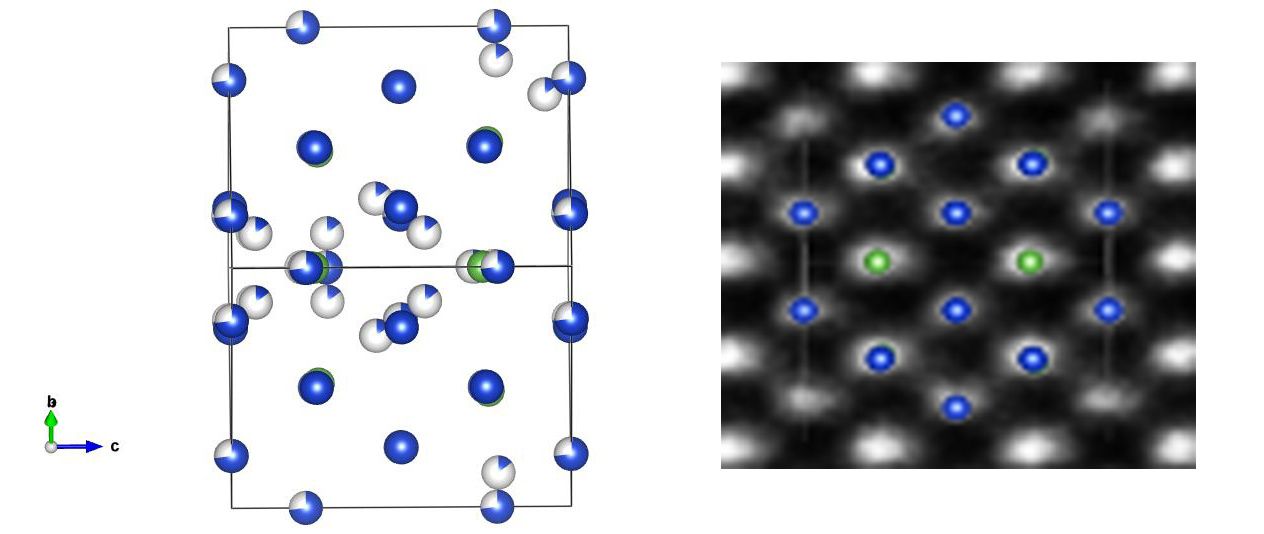
\includegraphics[width=0.9\linewidth]{mic_cu12as4s13_110} \\
  \end{minipage}

  \caption[HAADF изображение и теоретическая форма изображения рядов для образца Cu\textsubscript{12}As\textsubscript{4}S\textsubscript{13}]{HAADF изображение и теоретическая форма изображения рядов для образца Cu\textsubscript{12}As\textsubscript{4}S\textsubscript{13}}
    \label{img:mic3}
\end{figure}

На рисунке~\ref{img:xray} представлены: величина заселённости позиций атома Cu2 и изменение значения коэффициента атомарного смещения для позиции атома S2 в диапазоне температур от 85 до 293~К. Аномальное изменение значения коэффициента атомарного смещения для позиции атома S2, показывает наличие фазового перехода второго рода в диапазоне от 115 до 180 К.

\begin{figure}[ht]
  \begin{minipage}[ht]{0.5\linewidth}\centering
    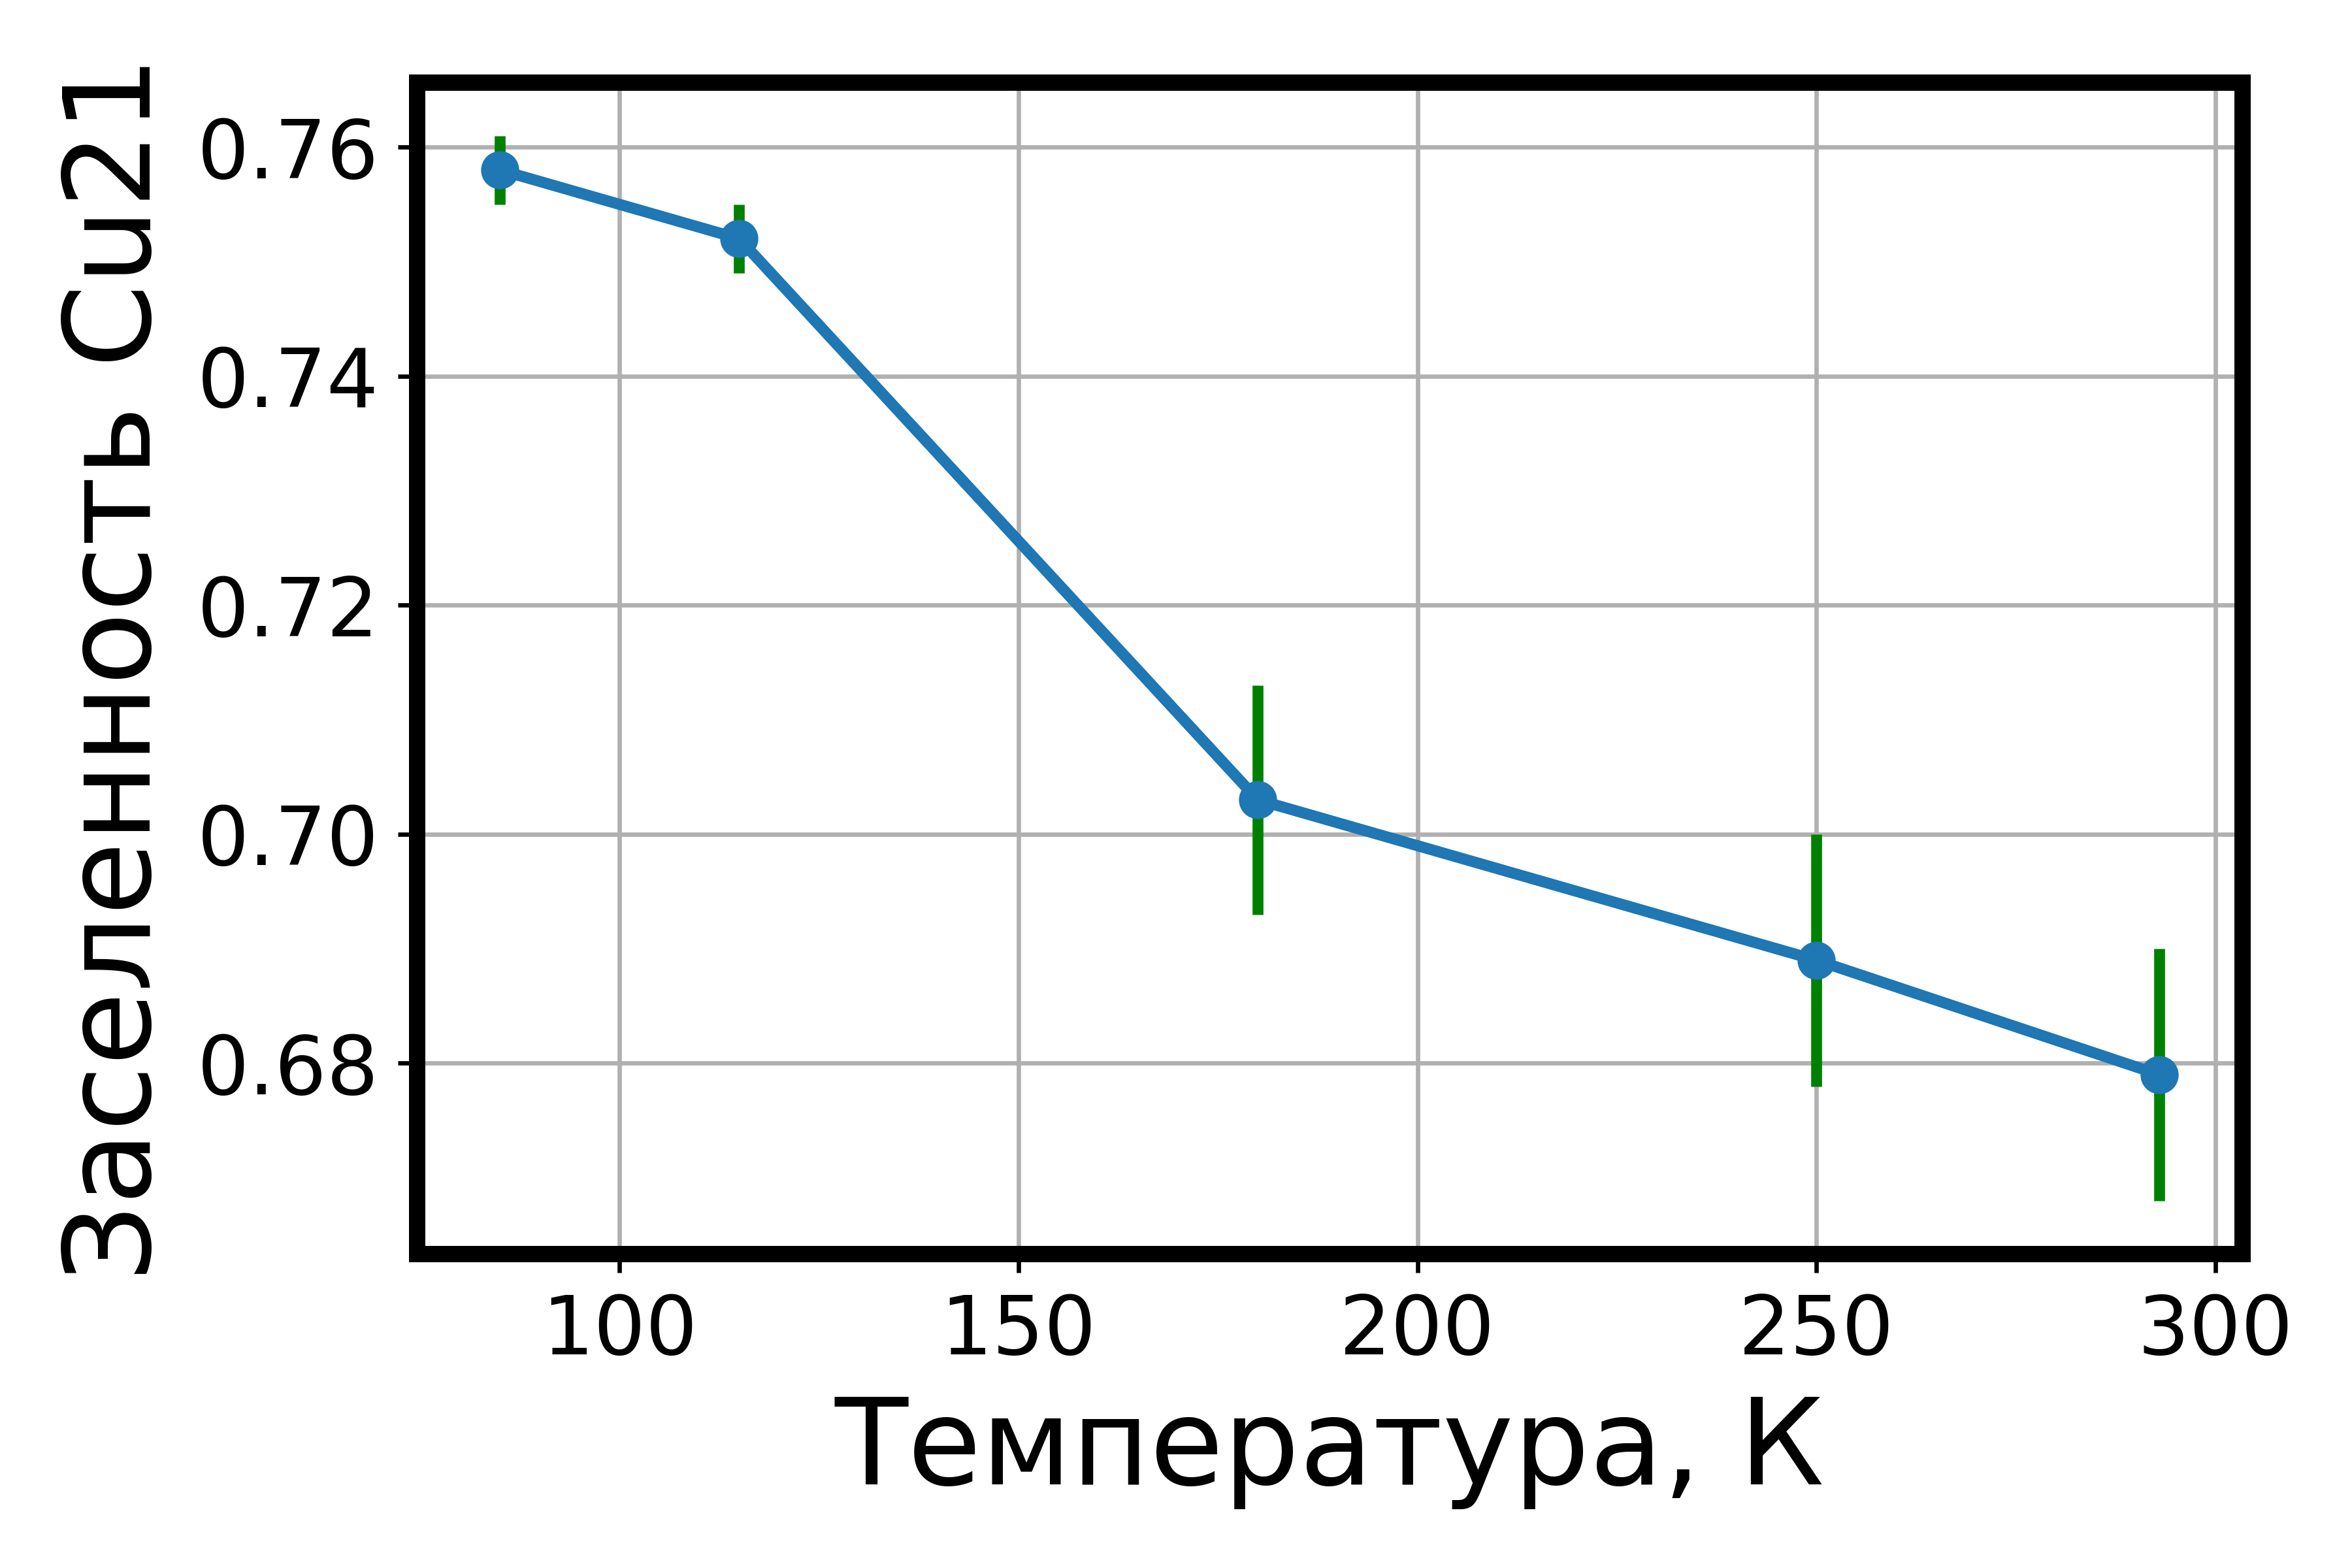
\includegraphics[width=0.9\linewidth]{structure_occCu2} \\ а)
  \end{minipage}
  \hfill
  \begin{minipage}[ht]{0.5\linewidth}\centering
    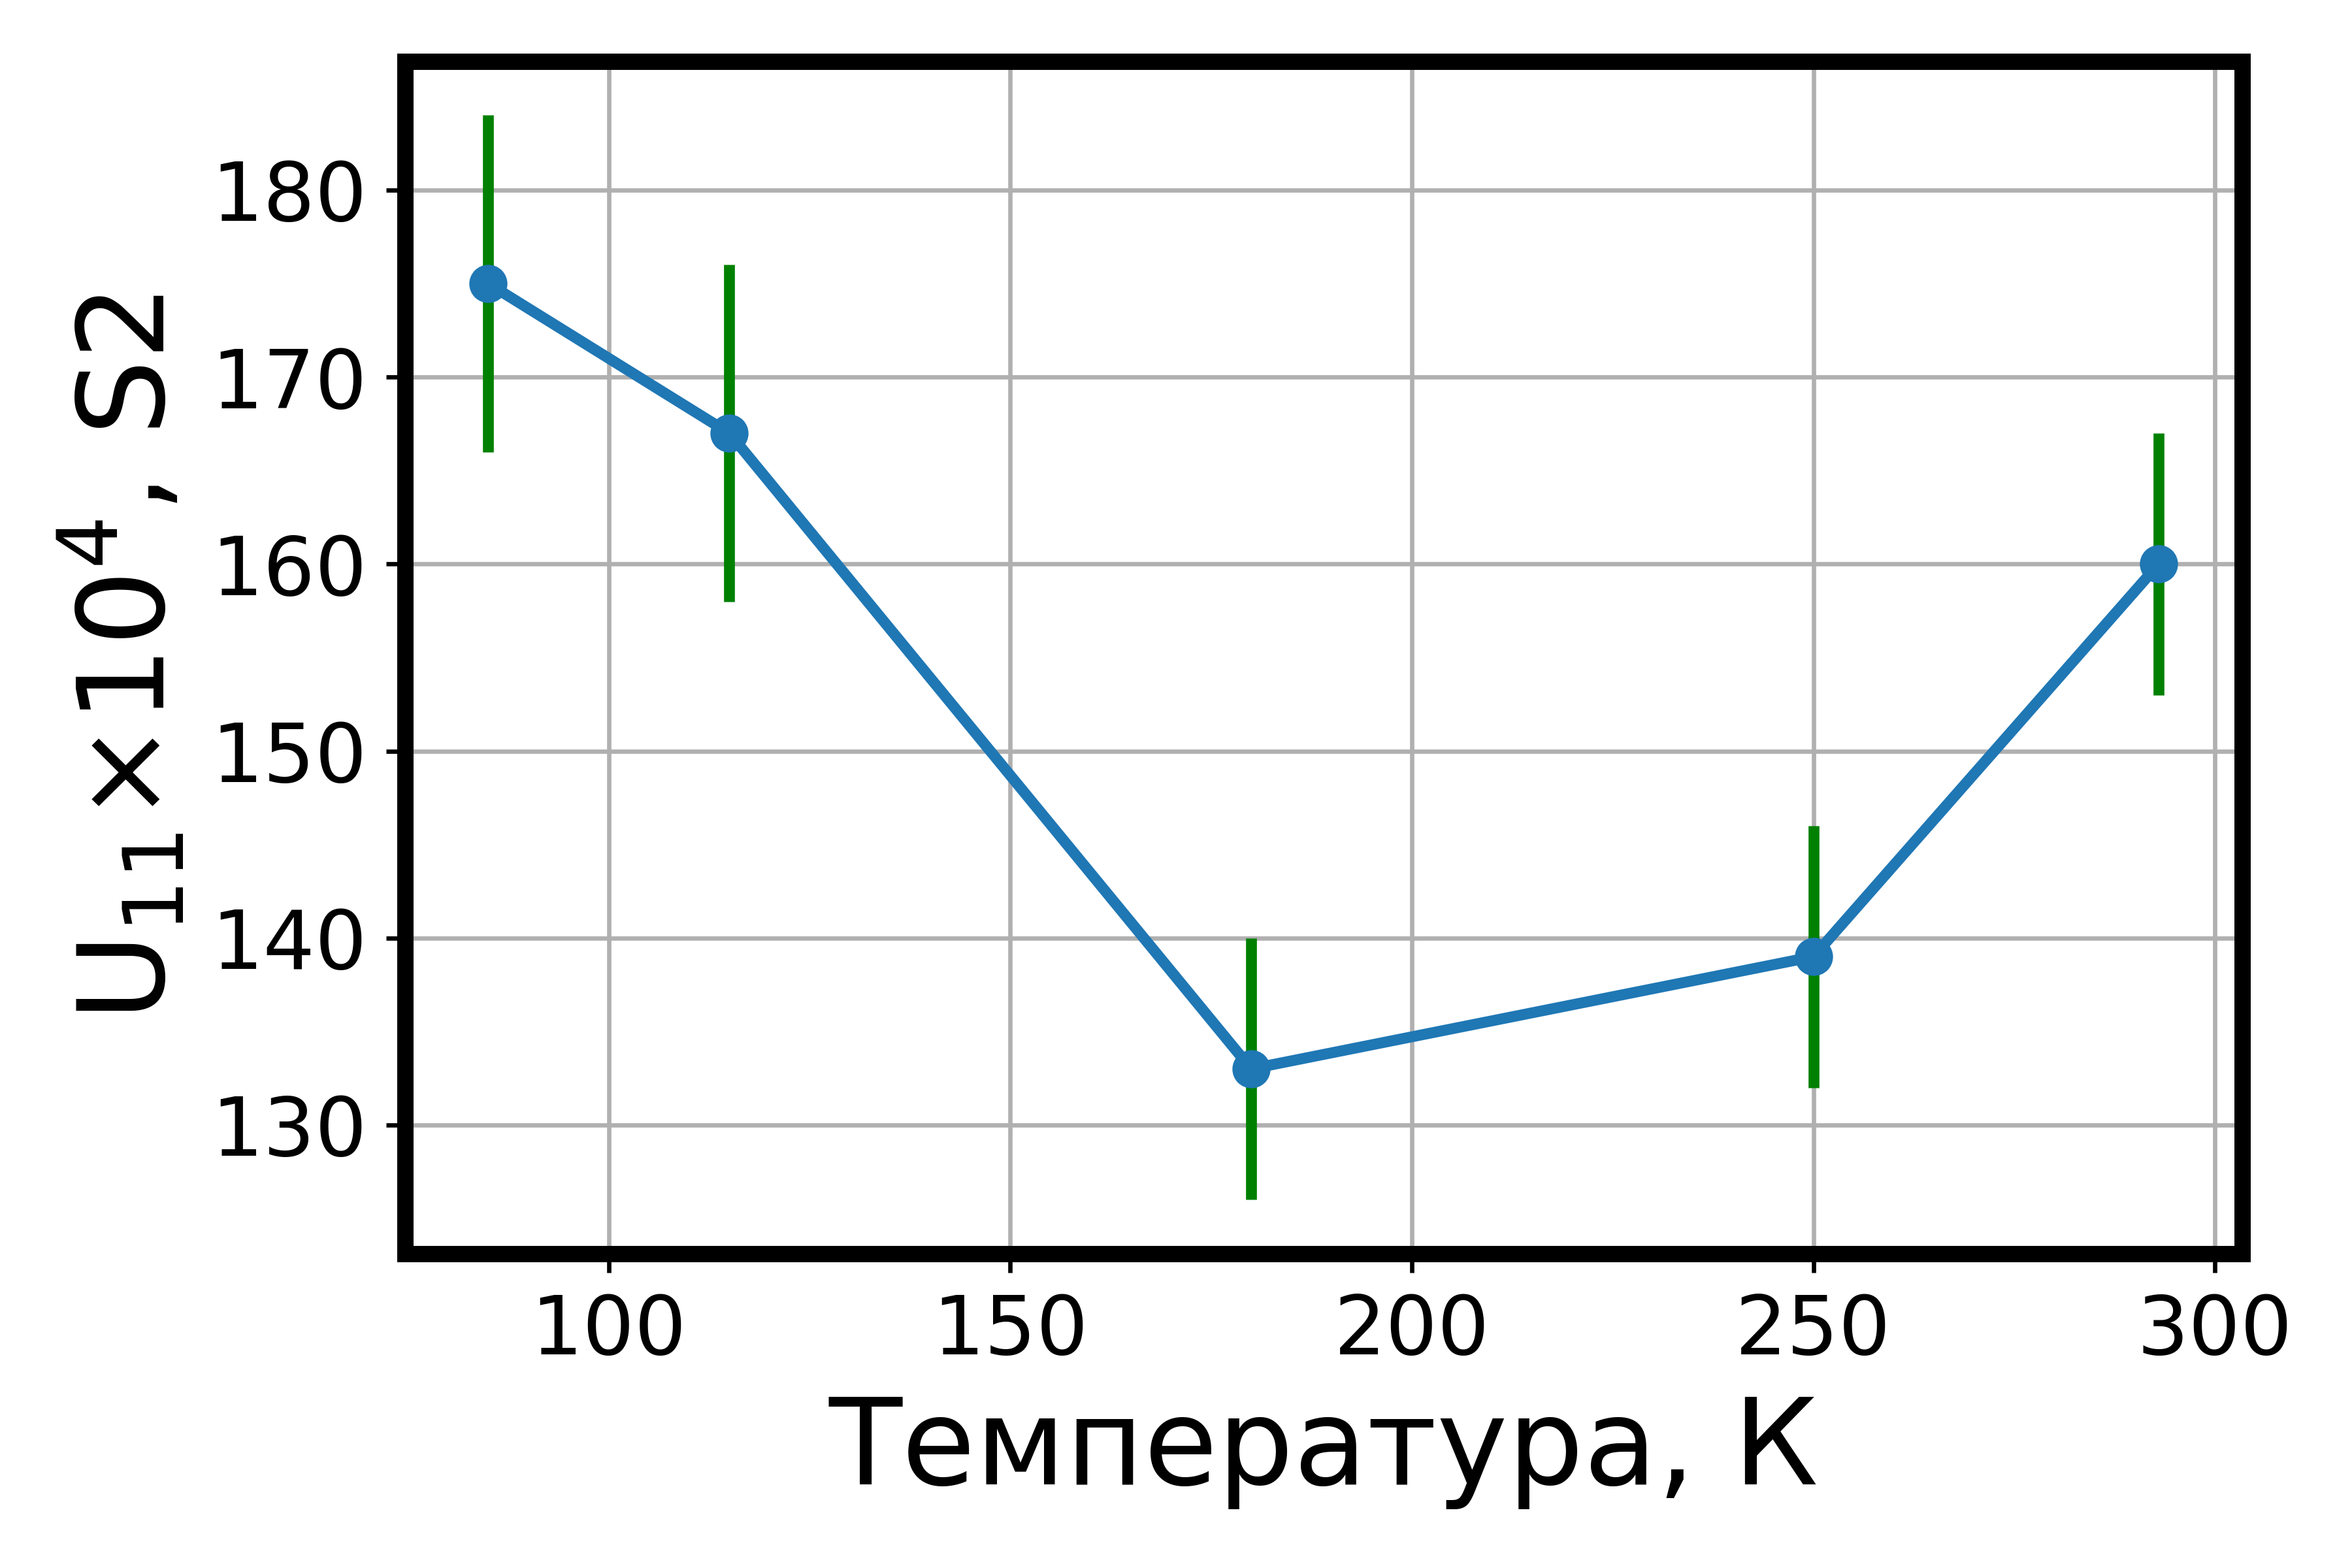
\includegraphics[width=0.9\linewidth]{structure_Ueq} \\ б)
  \end{minipage}

      \caption[Значение заселённости позиции атома Cu2 (а) и изменение значения коэффициента атомарного смещения для позиции атома S2 (б) в диапазоне температур от 85 до 293~К синтетического теннантита Cu\textsubscript{12}As\textsubscript{4}S\textsubscript{13}]{Значение заселённости позиции атома Cu2 (а) и изменение значения коэффициента атомарного смещения для позиции атома S2 (б) в диапазоне температур от 85 до 293~К синтетического теннантита Cu\textsubscript{12}As\textsubscript{4}S\textsubscript{13}}
    \label{img:xray}
\end{figure}

Рисунок \ref{img:xray2} представляет собой изображения распределений электронной плотности синтетического теннантита Cu\textsubscript{12}As\textsubscript{4}S\textsubscript{13} при температуре 293~(а) и 85~(б)~К в плоскости (011). По форме линий электронной плотности видно, что происходит полное разделение позиций Cu2 и Cu21. При комнатной температуре расстояние между Cu2 и Cu21 составляет 1.027(6)~$\angstrom$, при 85~К --- 1.108(5)~$\angstrom$. Расчёт энергий ФМ, АФМ, ПМ и диамагнитного состояний для экспериментально полученных структур показывает, что АФМ упорядочение в экспериментальной структуре при 85~К энергетически более выгодно, чем ферро- или пара- или диамагнитное состояния при этой же температуре. Для экспериментальной структуры при 293~К ФМ, АФМ, ПМ конфигурации имеют одинаковую (до 4 знака) энергию, что указывает на их одинаковую выгодность.

\begin{figure}[ht]
  \begin{minipage}[ht]{0.5\linewidth}\centering
    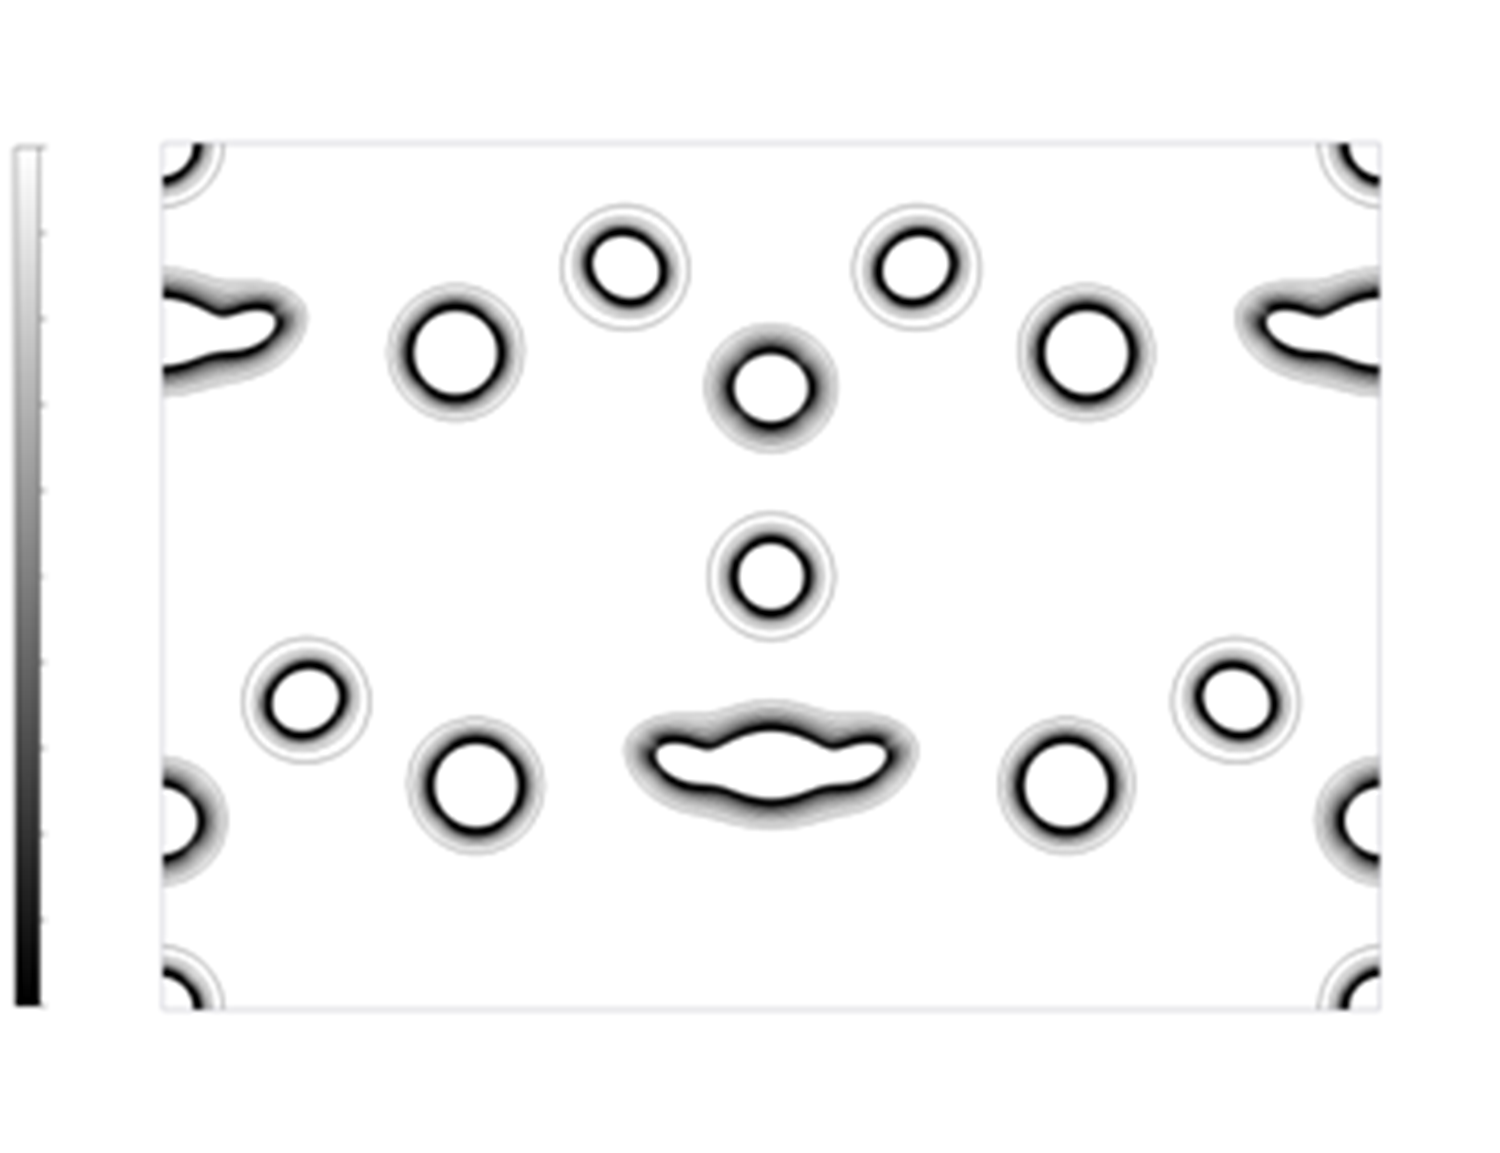
\includegraphics[width=0.9\linewidth]{Electron_density_293.png} \\ а)
  \end{minipage}
  \hfill
  \begin{minipage}[ht]{0.5\linewidth}\centering
    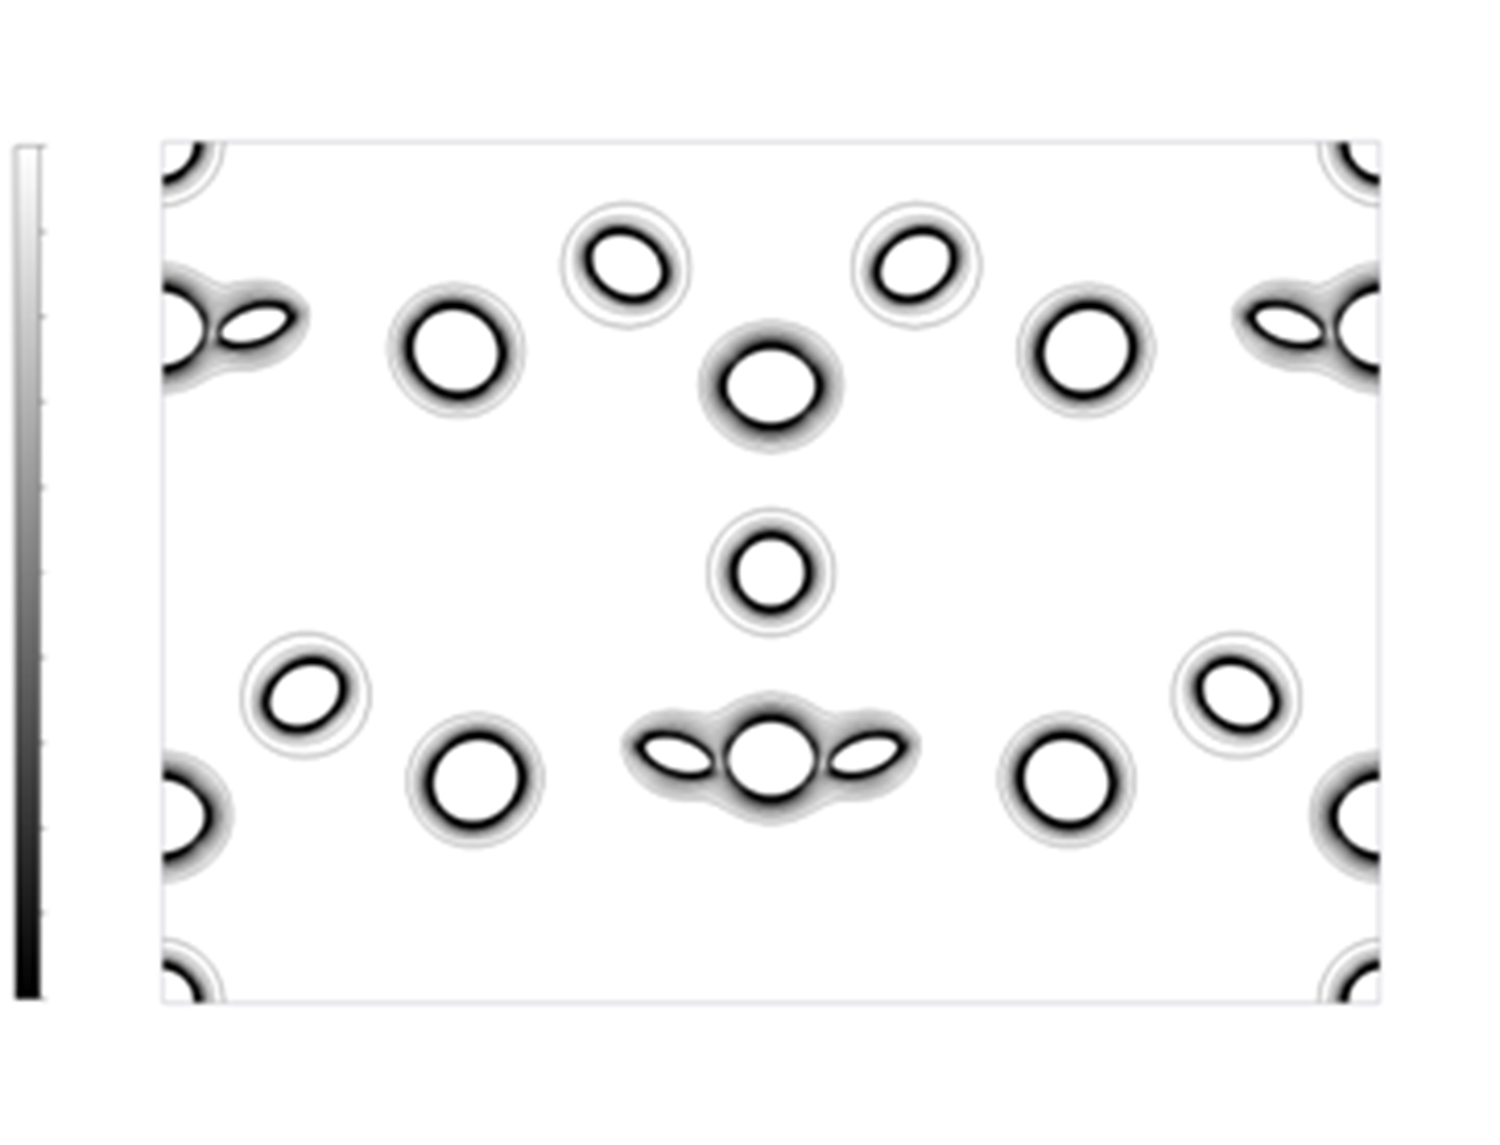
\includegraphics[width=0.9\linewidth]{Electron_density_85.png} \\ б)
  \end{minipage}

      \caption[Распределение электронной плотности при температуре 293~(а) и 85~(б)~К в плоскости (011) синтетического теннантита Cu\textsubscript{12}As\textsubscript{4}S\textsubscript{13}]{Распределение электронной плотности при температуре 293~(а) и 85~(б)~К в плоскости (011) синтетического теннантита Cu\textsubscript{12}As\textsubscript{4}S\textsubscript{13}}
    \label{img:xray2}
\end{figure}


По данным первопринципных расчётов энергий элементарных ячеек для синтетического теннантита Cu\textsubscript{12}As\textsubscript{4}S\textsubscript{13} следует,  что смещение атома меди в лавесовсом полиэдре может приводить как к увеличению энергии ячейки, так и её к уменьшению.
Результаты показывают, что существующее неэквивалентное  окружение атомов меди в позициях Cu21 и Cu2 ведет к возникновению разного химического потенциала для структур с разным расположением атомов меди (анализировались позиции Cu21 и Cu2) и, вероятно, является движущей силой для возникновения позиции Cu21. Расстояние между сдвинутым атомом и его идеальным положением в лавесовсом полиэдре для наиболее энергетически выгодной элементарной ячейки составляет 0.6~$\angstrom$, по экспериментальным данным --- 1.027(6)~$\angstrom$.
Анализ распределения электрических зарядов указывает, что для более выгодных с энергетической точки зрения структур не возникает разной валентности на атомах меди Cu1,
но появляется разность зарядов для позиций атомов Cu2 (Cu21) (варианты структур с 11 по 15). Также стоит отметить, что структуры, где сдвинуты все 6 атомов меди, обладают большей энергией элементарной ячейки в сравнении с энергией идеального полиэдра и представляют не самые энергетически выгодные конфигурации  (варианты 5--10).




%\begin{figure}[p!]
%\centering
 % \begin{minipage}[ht]{0.7\linewidth}\centering
 %   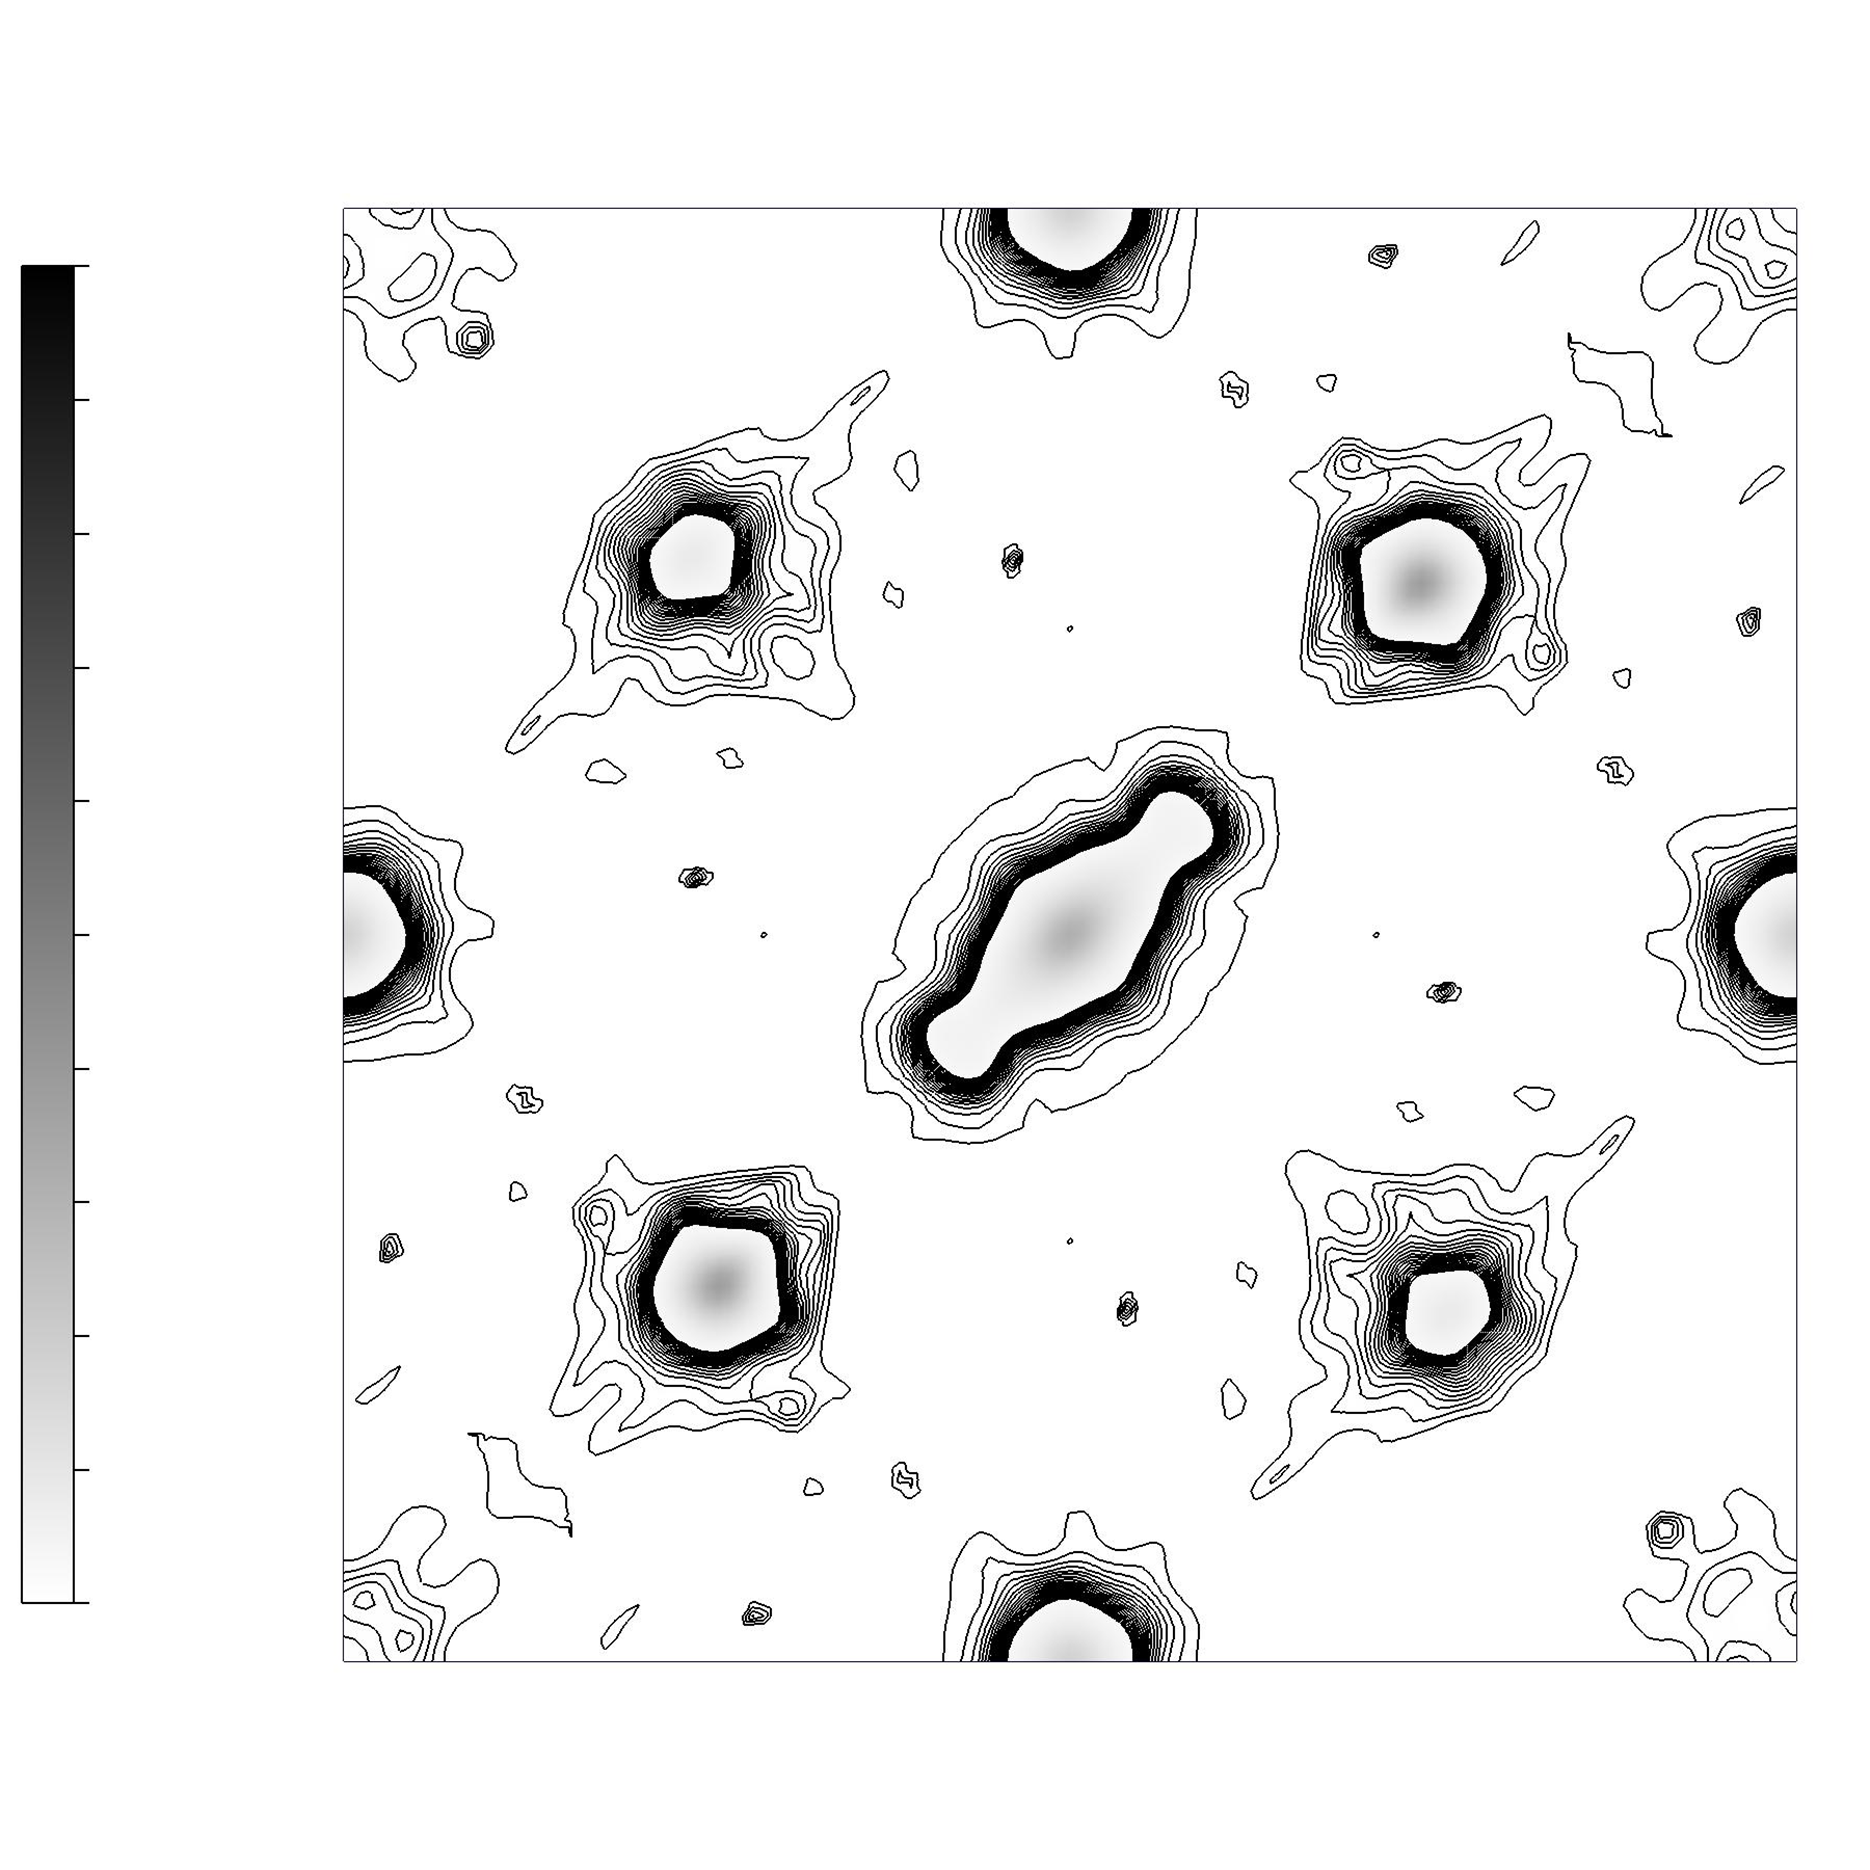
\includegraphics[width=0.9\linewidth]{Electron_density_As} \\ а)
 % \end{minipage}
 % \vfill
 % \begin{minipage}[ht]{0.7\linewidth}\centering
 %   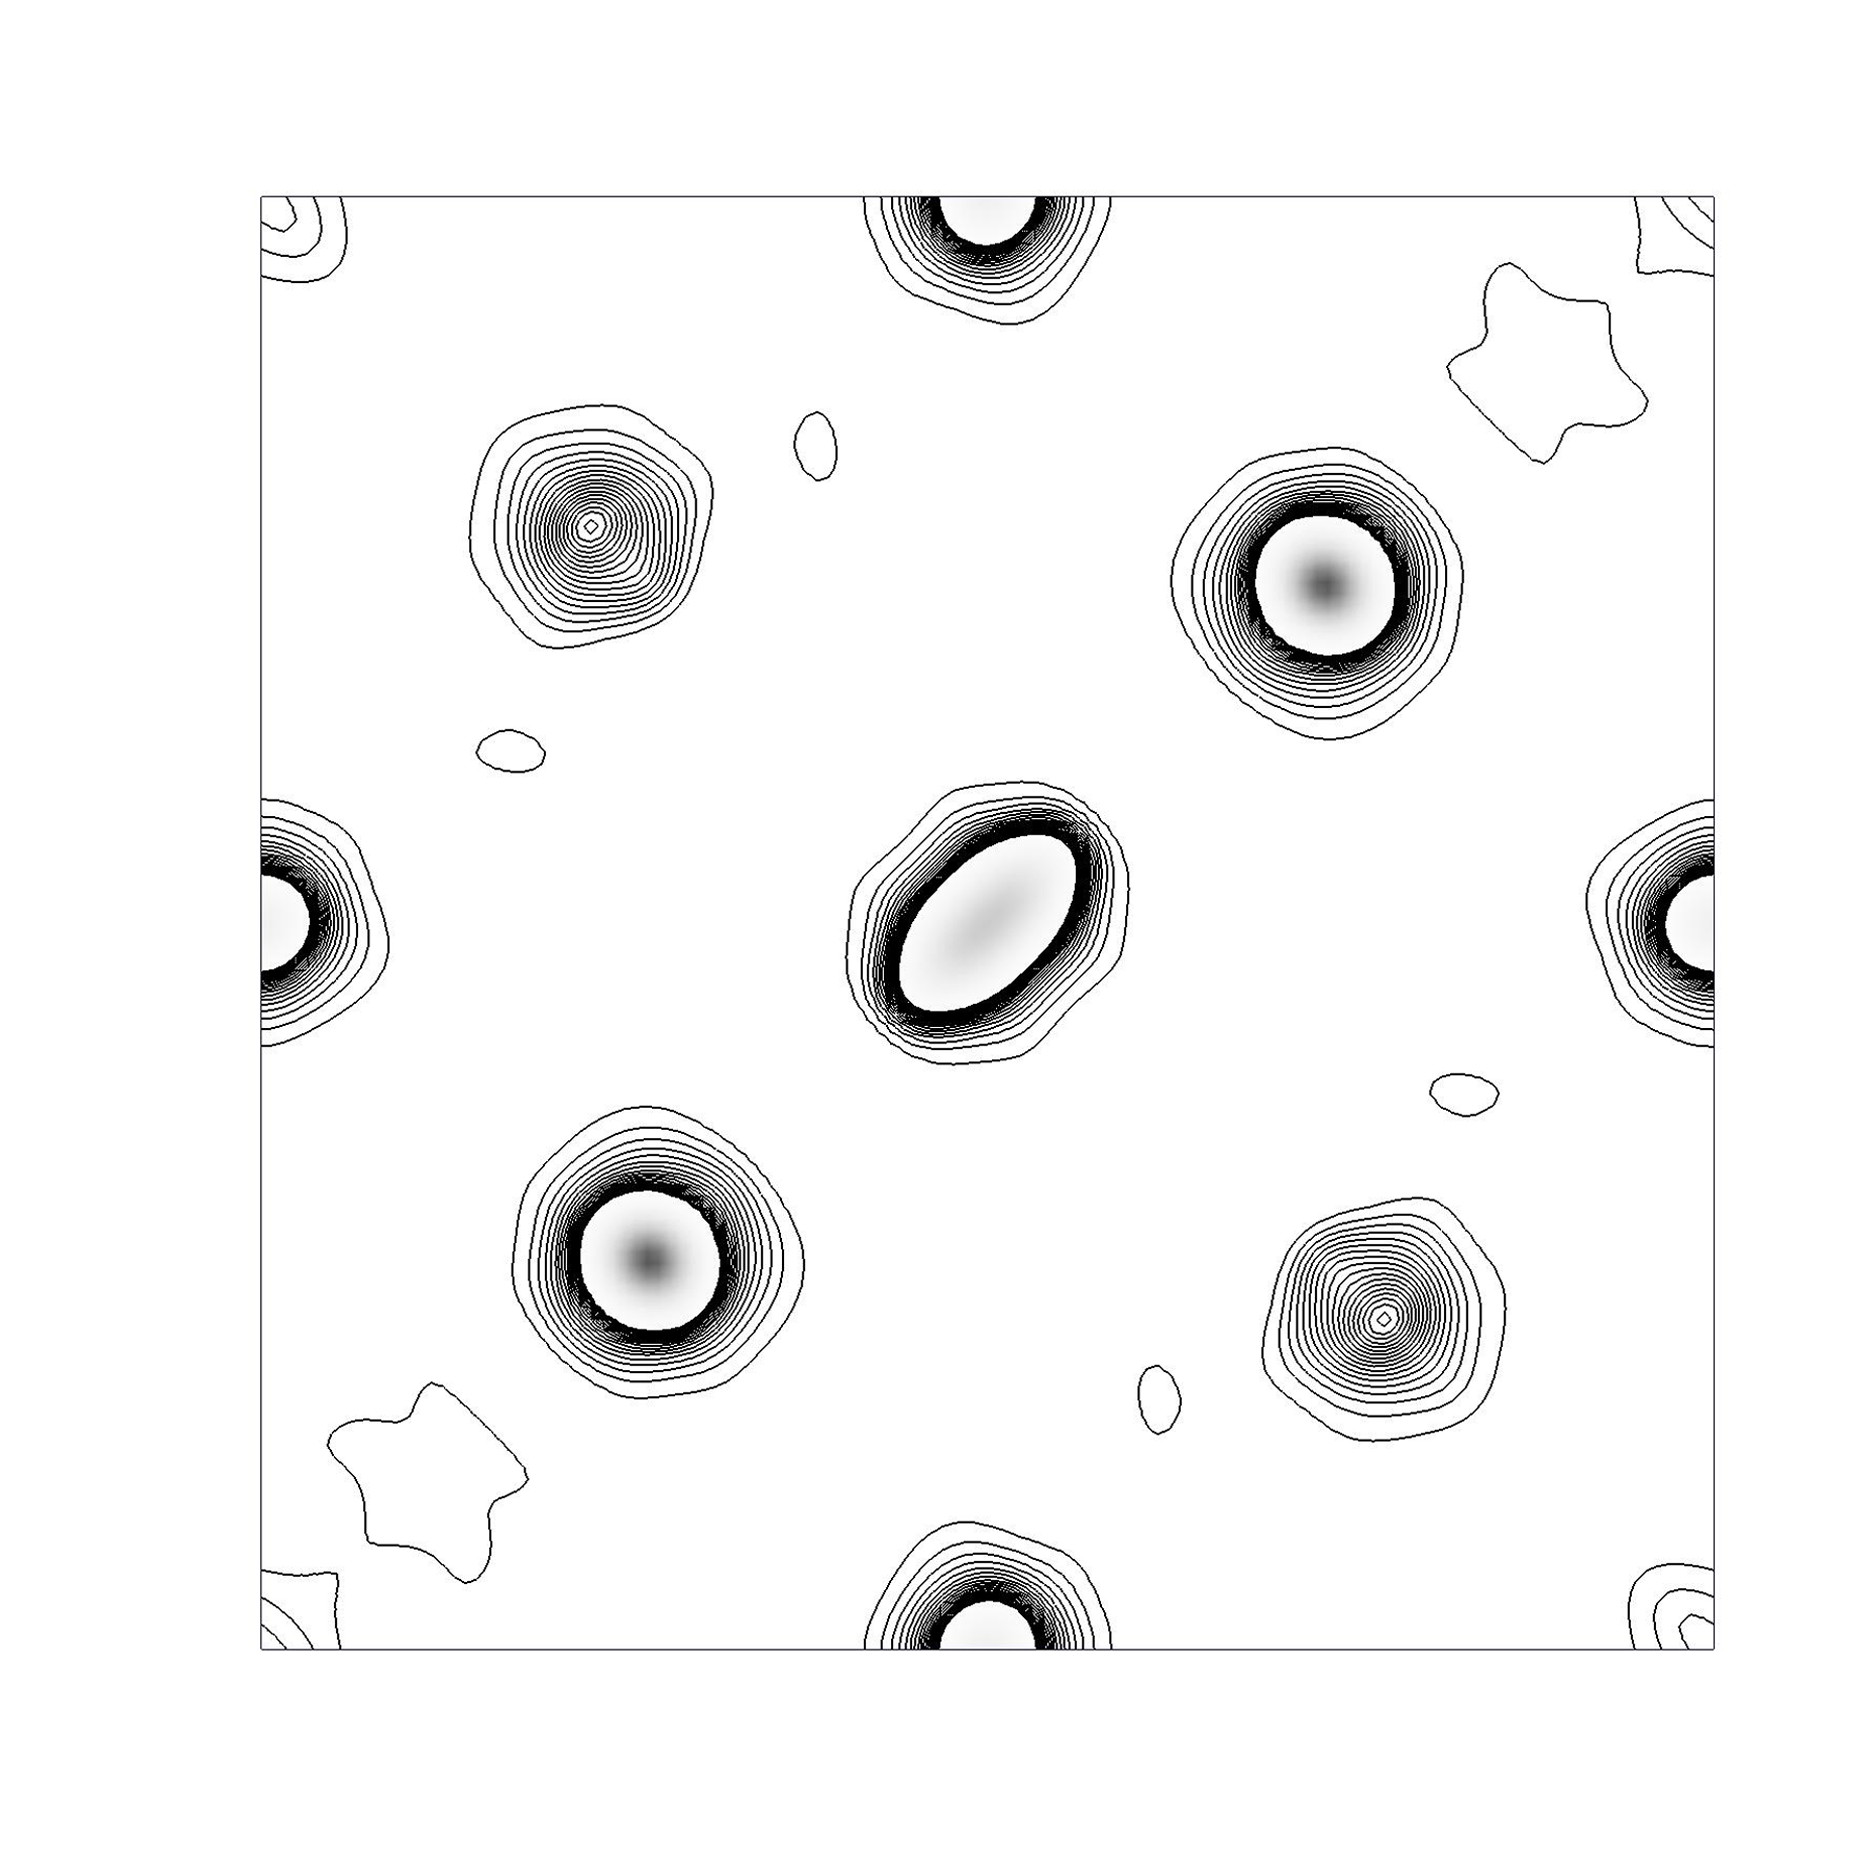
\includegraphics[width=0.9\linewidth]{Electron_density_Sb} \\ б)
 % \end{minipage}
 % \caption[Электронная плотность синтетического теннантита Cu\textsubscript{12}As\textsubscript{4}S\textsubscript{13} и тетраэдрита Cu\textsubscript{12}Sb\textsubscript{4}S\textsubscript{13}]{Электронная плотность синтетического теннантита Cu\textsubscript{12}As\textsubscript{4}S\textsubscript{13} и тетраэдрита Cu\textsubscript{12}Sb\textsubscript{4}S\textsubscript{13}}
  %  \label{img:figure2}
%\end{figure}





\clearpage

\newpage
     % Глава 3
 \chapter{Обсуждение экспериментальных результатов} \label{chapt4}
В данной главе представлены результаты экспериментальных исследований структуры и квантовомеханических расчётов синтетического теннантита Cu\textsubscript{12}As\textsubscript{4}S\textsubscript{13}, исследование зависимостей намагниченности в диапазоне температур от 2 до 350~К и спектров комбинационного рассеяния света для соединений при комнатной температуре Cu\textsubscript{12}As\textsubscript{4}S\textsubscript{13}, Cu\textsubscript{12}Sb\textsubscript{4}S\textsubscript{13}, Cu\textsubscript{3}AsSe\textsubscript{3} и Cu\textsubscript{3}SbSe\textsubscript{3}. А также измерение телоёмкости в диапазоне температур от 4 до 350~К и результаты моделирования теплоёмкости для Cu\textsubscript{12}As\textsubscript{4}S\textsubscript{13} и Cu\textsubscript{3}AsSe\textsubscript{3}.
Экспериментальные результаты рассматриваются в контексте опубликованных научных литературных данных. Кроме того, в главе отмечаются пути дальнейшего исследования синтезированных соединений.

Анализ результатов начинается с обсуждения особенностей структуры синтетического теннантита в диапазоне температур от 100 до 300~К, особенностей экспериментальной и расчётной теплоёмкости в диапазоне температур от 2 до 350~К и закономерностей изменения магнитных свойств при изовалентном замещении в сложных халькогенидах меди в диапазоне температур от 2 до 350~К.

\section{Рентгеноструктурный анализ синтетического теннантита и результаты квантовомеханических расчётов} \label{sect4_1}

По результатам рентгеноструктурного анализа монокристаллического образца синтетического теннантита Cu\textsubscript{12}As\textsubscript{4}S\textsubscript{13} при комнатной температуре обнаружено, что значение суммы заселённостей позиций атомов Cu2 и Cu21 составляет 1, а не 1.04 как опубликовано ранее\cite{Makovicky_2006}.
Полученные результаты показывают, что на структурную формулу синтетического теннантита приходится 12 атомов меди, а не 12.5.
Таким образом, лавесовский полиэдр состоит из 6 атомов меди.
Разное значение эллиптичности рядов, определенное при анализе плоскости (011) атомарного изображения монокристаллического образца синтетического теннантита Cu\textsubscript{12}As\textsubscript{4}S\textsubscript{13} (Рис.~\ref{img:mic}), говорит в пользу существования позиции меди Cu21 в структуре теннантите, что согласуется с результатами рентгеноструктурного анализа описанного выше. Произвести количественный анализ изображения не удалось.



На рисунке~\ref{img:xray} представлены: величина заселенности позиций атома Cu2 и изменение значения коэффициента атомарного смещения для позиции атома S2 в диапазоне температур от 85 до 293~К. Аномальное изменение значения коэффициента атомарного смещения для позиции атома S2, показывает наличие фазового перехода 2 рода в диапазоне от 115 до 180 К.

\begin{figure}[ht]
  \begin{minipage}[ht]{0.5\linewidth}\centering
    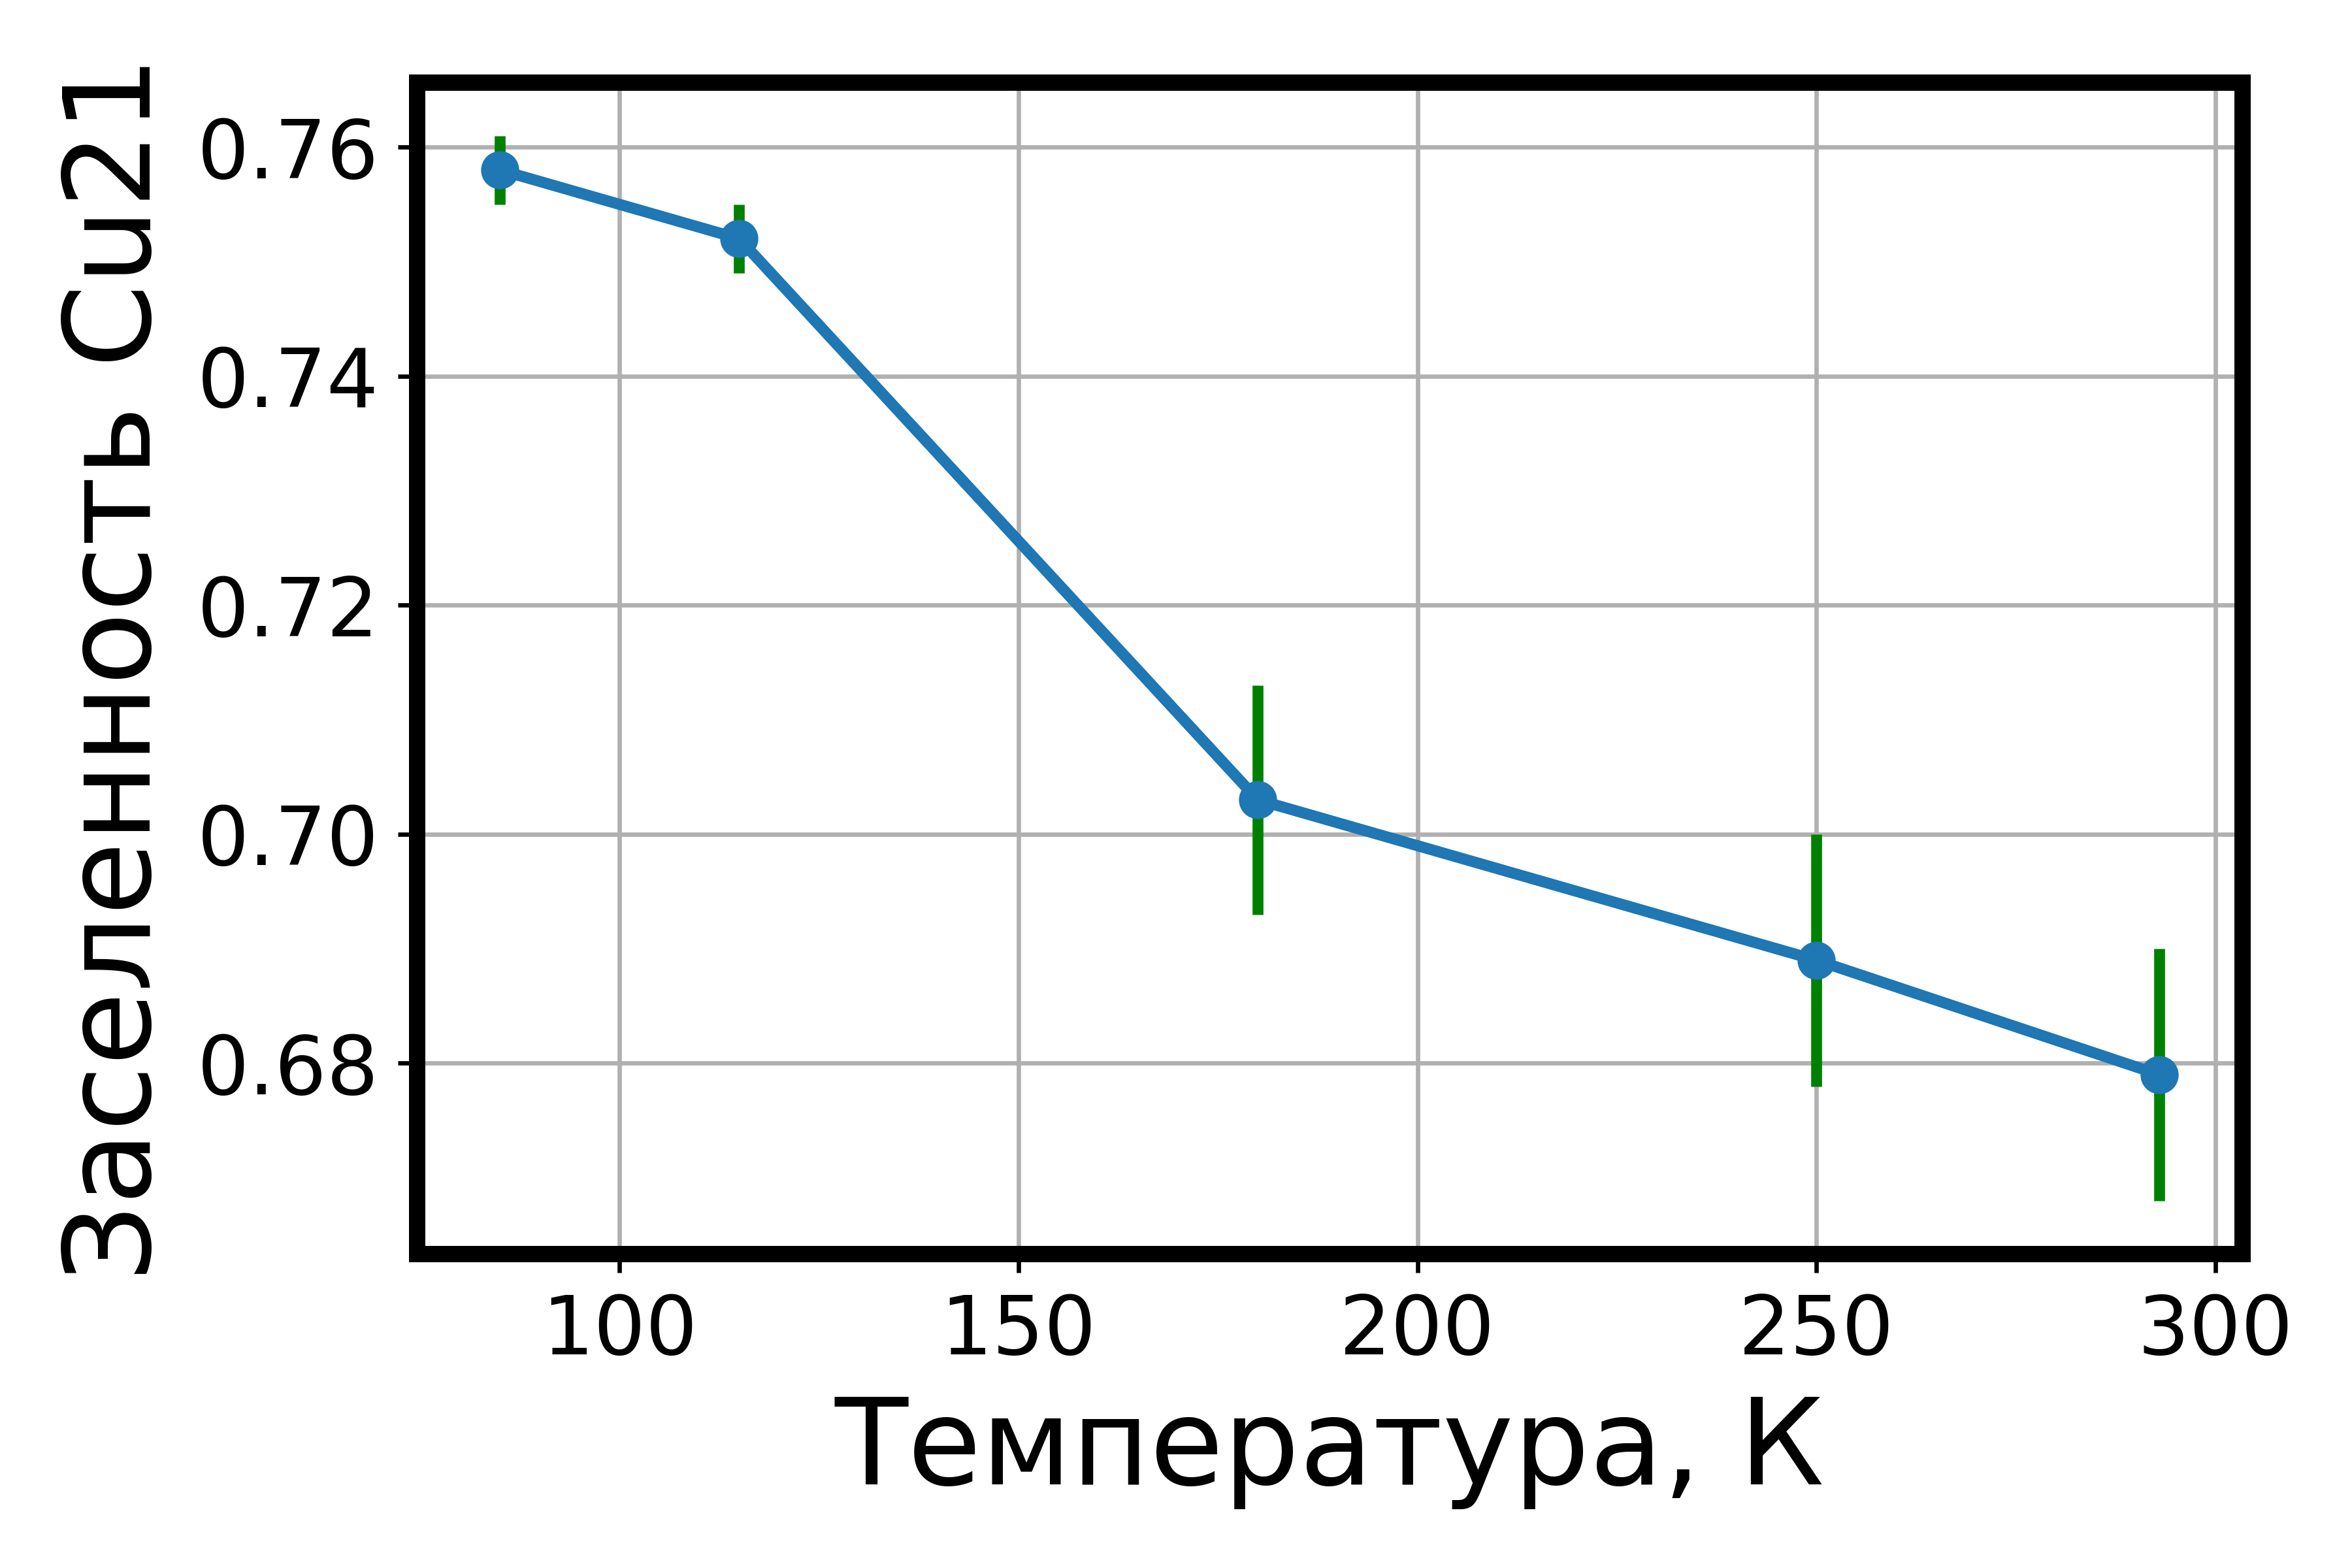
\includegraphics[width=0.9\linewidth]{structure_occCu2} \\ а)
  \end{minipage}
  \hfill
  \begin{minipage}[ht]{0.5\linewidth}\centering
    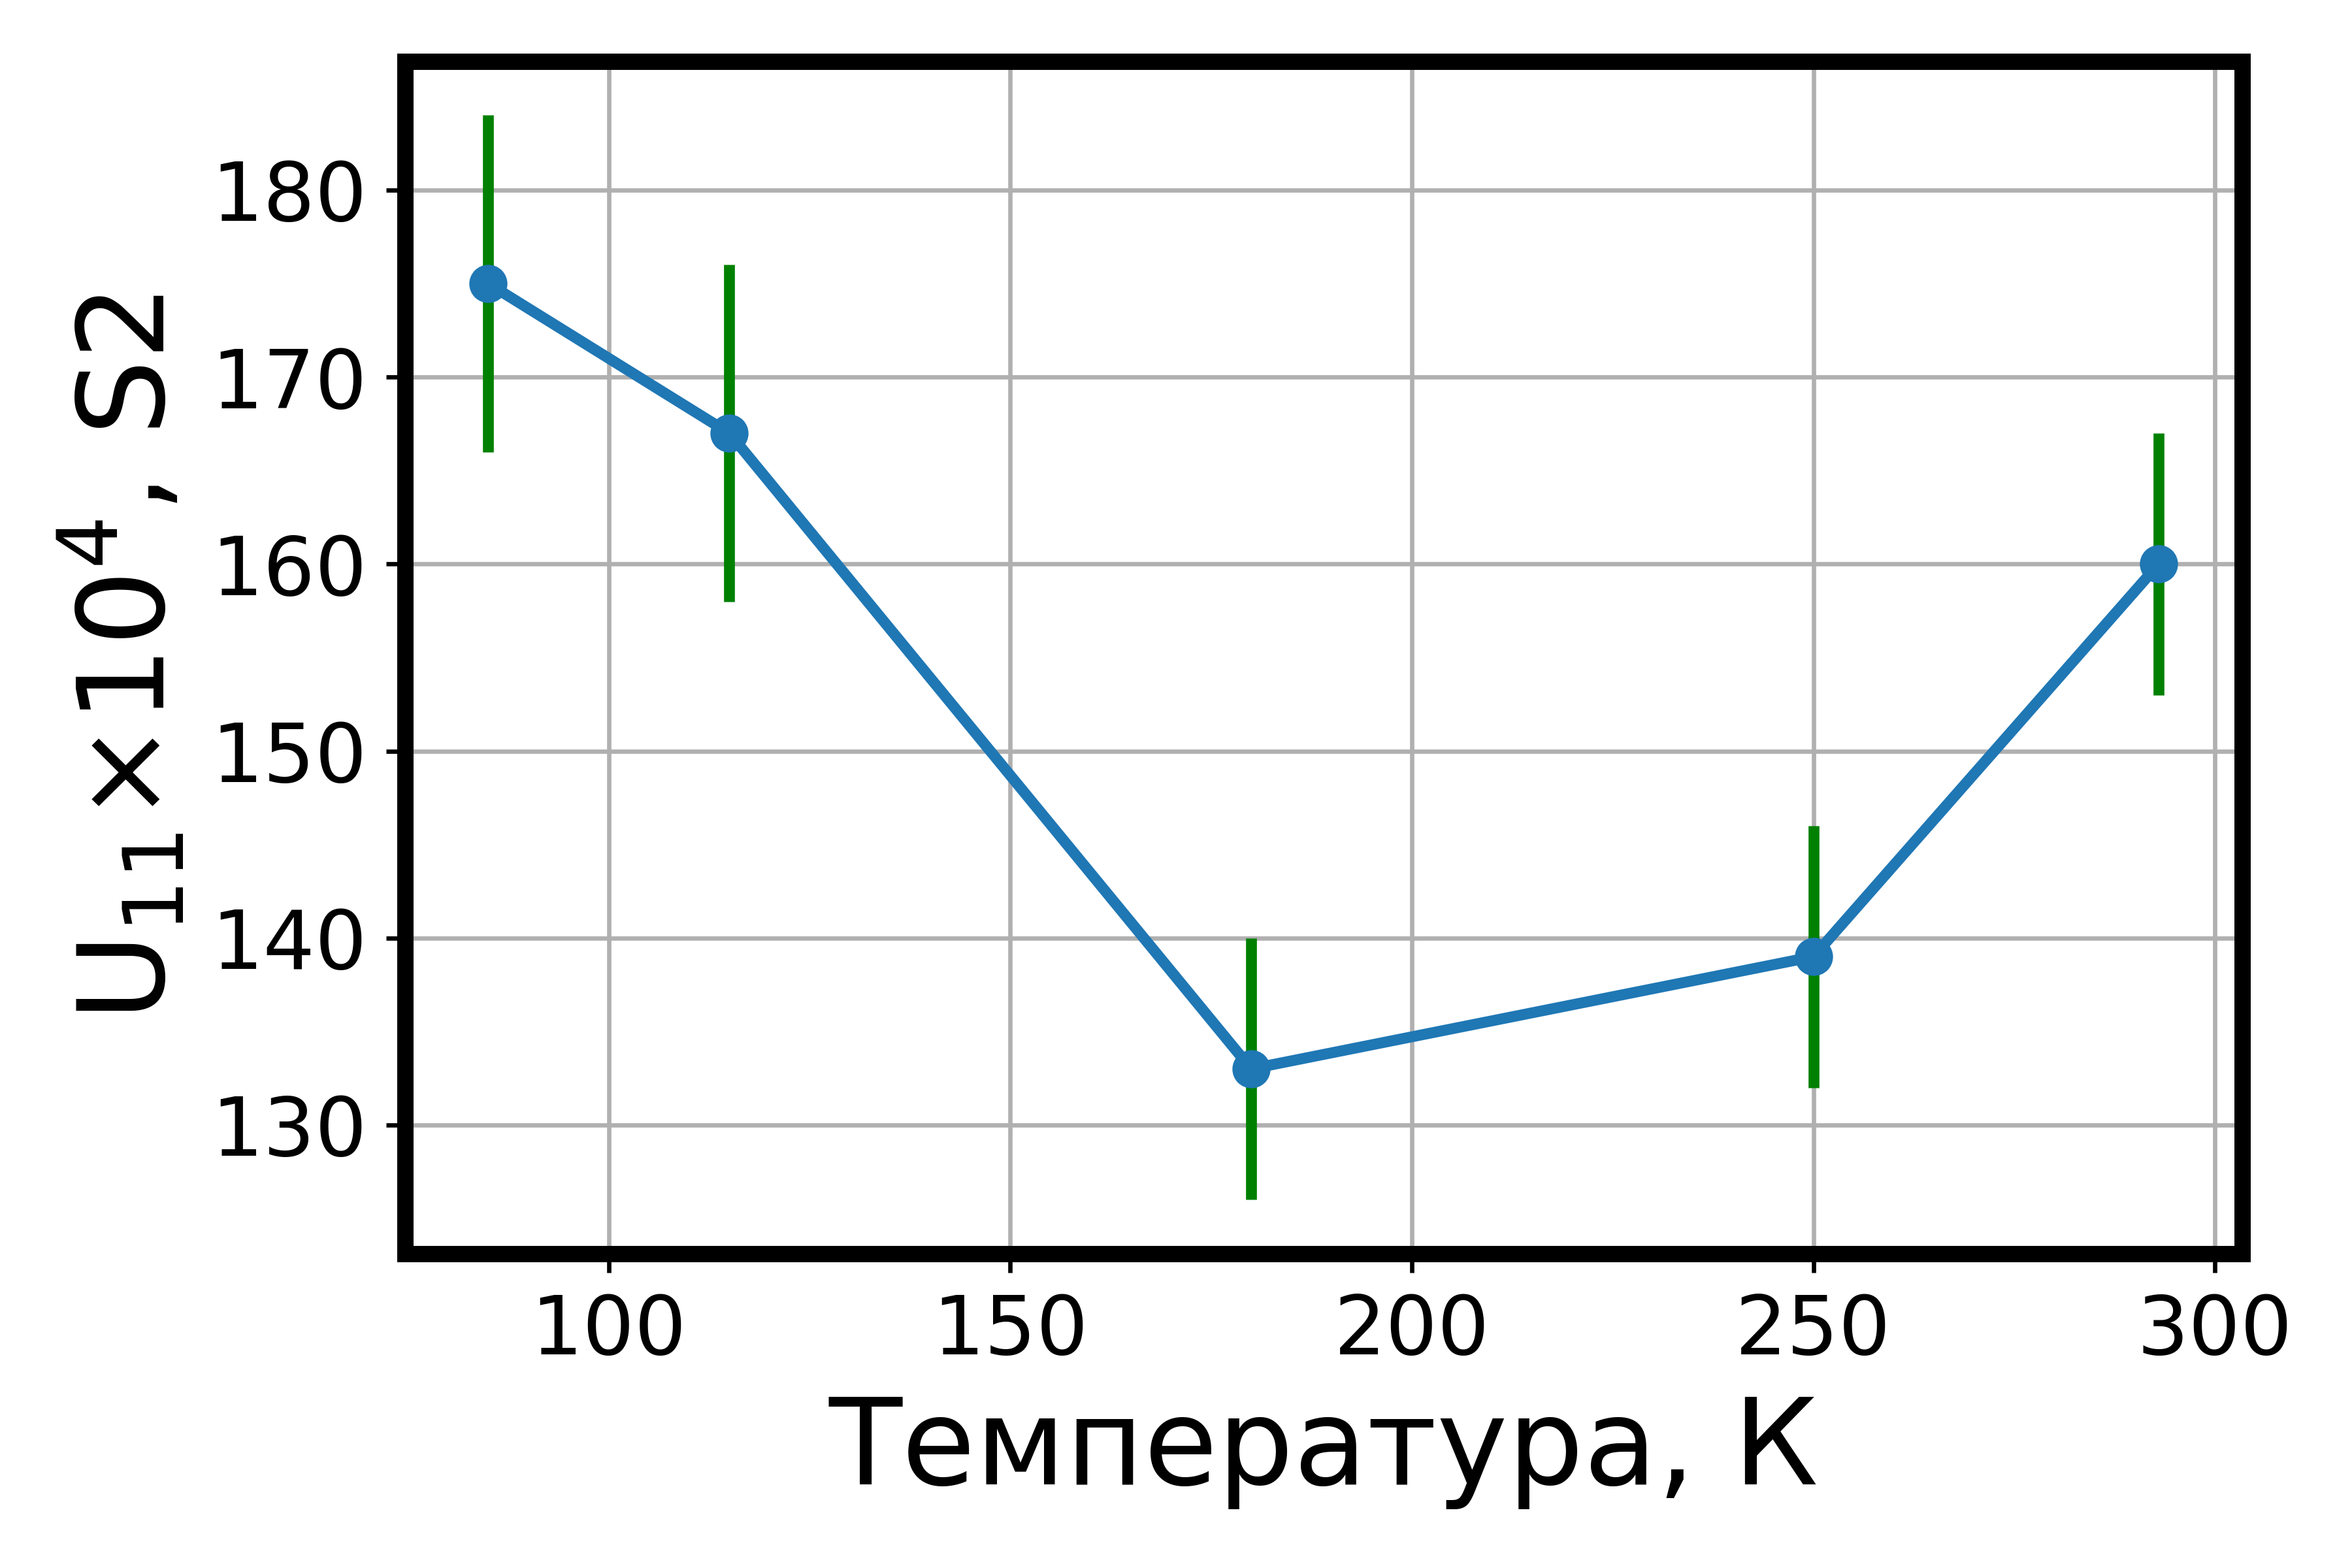
\includegraphics[width=0.9\linewidth]{structure_Ueq} \\ б)
  \end{minipage}

      \caption[Значение заселенности позиции атома Cu2 (а) и изменение значения коэффициента атомарного смещения для позиции атома S2 (б) в диапазоне температур от 85 до 293~К синтетического теннантита Cu\textsubscript{12}As\textsubscript{4}S\textsubscript{13}]{Значение заселенности позиции атома Cu2 (а) и изменение значения коэффициента атомарного смещения для позиции атома S2 (б) в диапазоне температур от 85 до 293~К синтетического теннантита Cu\textsubscript{12}As\textsubscript{4}S\textsubscript{13}}
    \label{img:xray}
\end{figure}

Рисунок \ref{img:xray2} представляет собой изображения распределений электронной плотности синтетического теннантита Cu\textsubscript{12}As\textsubscript{4}S\textsubscript{13} при температуре 293~(а) и 85~(б)~К в плоскости (011). По форме линий электронной плотности видно, что происходит полное разделение позиций Cu2 и Cu21. При комнатной температуре расстояние между Cu2 и Cu21 составляет 1.027(6)~$\angstrom$, при 85~К --- 1.108(5)~$\angstrom$. Расчёт энергий ФМ, АФМ, ПМ и диамагнитного состояний для экспериментально полученных структур показывает, что АФМ упорядочение в экспериментальной структуре при 85~К энергетически более выгодно, чем ферро- или пара- или диамагнитное состояния при этой же температуре. Для экспериментальной структуры при 293~К ФМ, АФМ, ПМ конфигурации имеют одинаковую (до 4 знака) энергию, что указывает на их одинаковую выгодность.

\begin{figure}[ht]
  \begin{minipage}[ht]{0.5\linewidth}\centering
    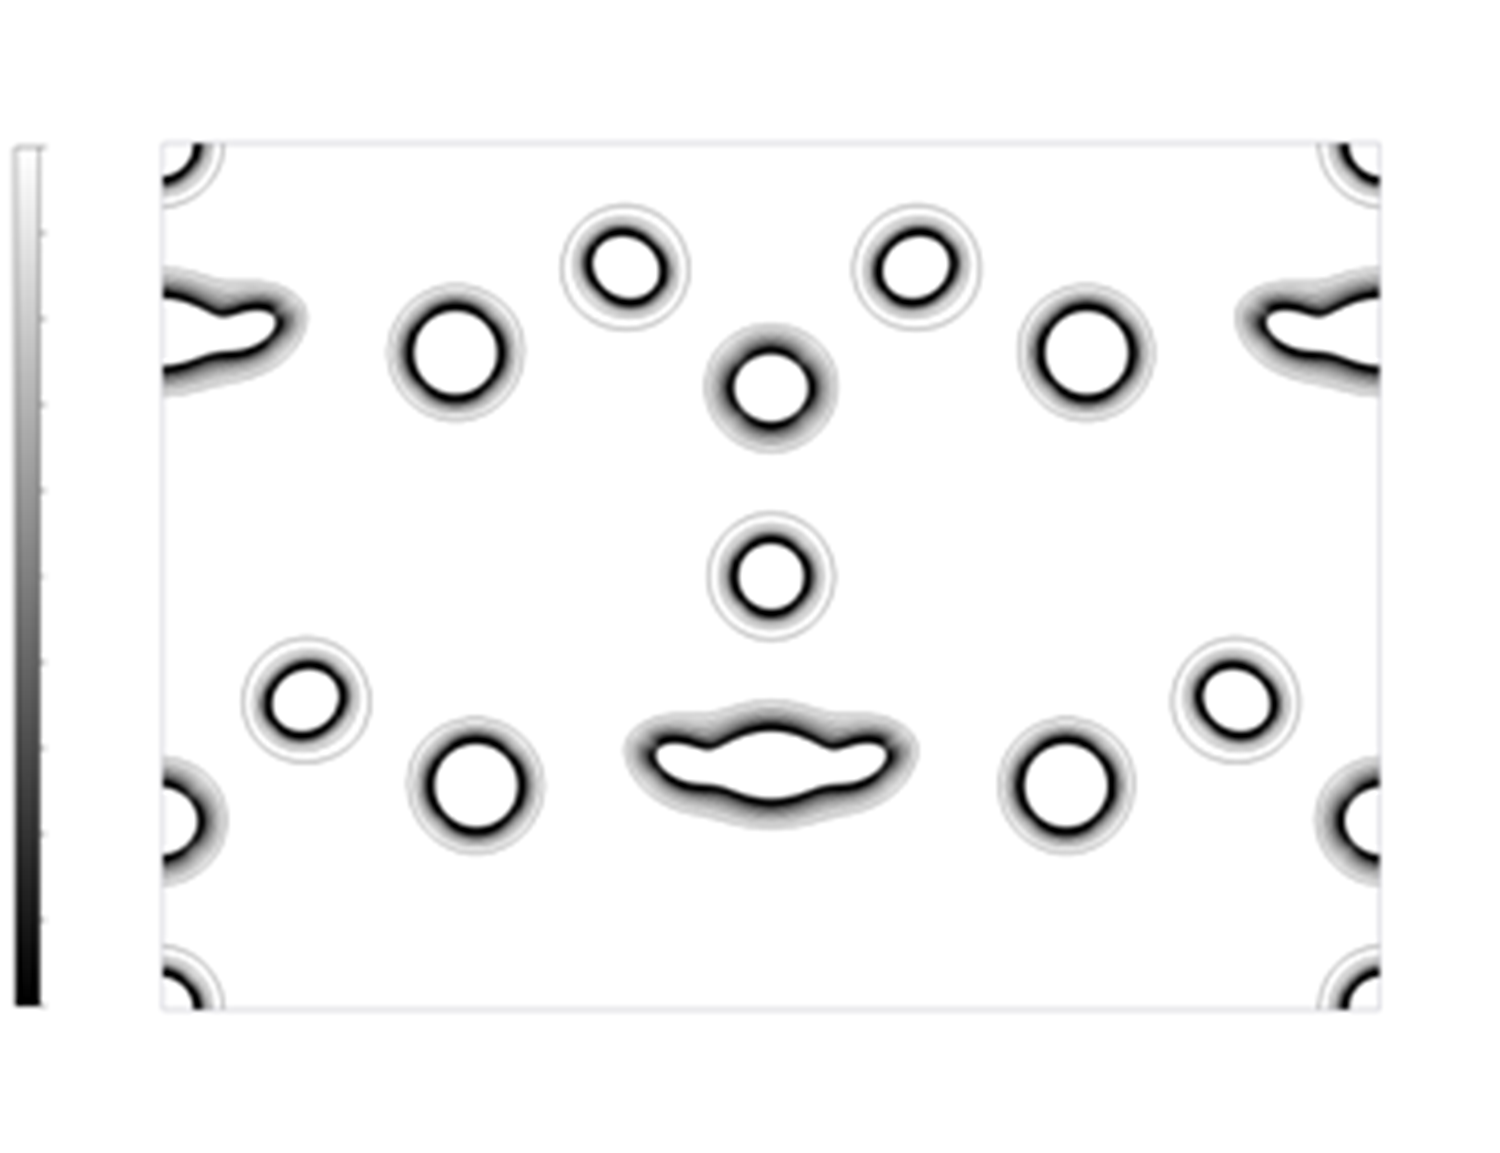
\includegraphics[width=0.9\linewidth]{Electron_density_293.png} \\ а)
  \end{minipage}
  \hfill
  \begin{minipage}[ht]{0.5\linewidth}\centering
    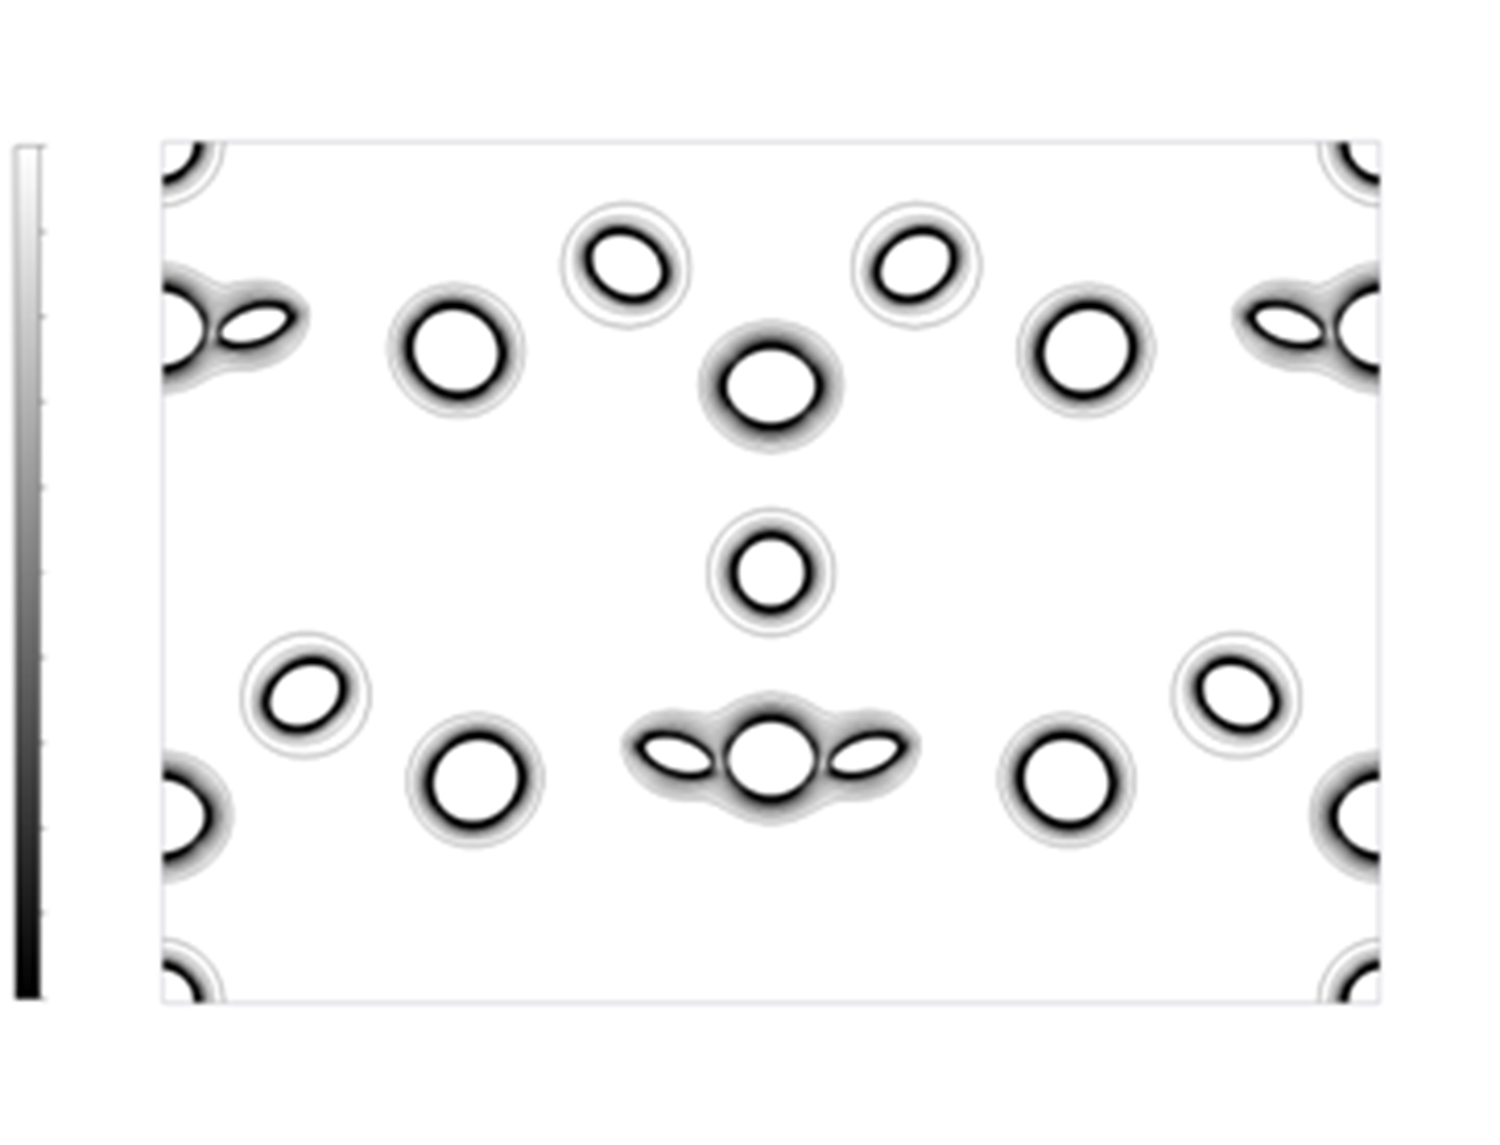
\includegraphics[width=0.9\linewidth]{Electron_density_85.png} \\ б)
  \end{minipage}

      \caption[Распределение электронной плотности при температуре 293~(а) и 85~(б)~К в плоскости (011) синтетического теннантита Cu\textsubscript{12}As\textsubscript{4}S\textsubscript{13}]{Распределение электронной плотности при температуре 293~(а) и 85~(б)~К в плоскости (011) синтетического теннантита Cu\textsubscript{12}As\textsubscript{4}S\textsubscript{13}}
    \label{img:xray2}
\end{figure}


По данным первопринципных расчётов энергий элементарных ячеек для синтетического теннантита Cu\textsubscript{12}As\textsubscript{4}S\textsubscript{13} следует,  что смещение атома меди в лавесовсом полиэдре может приводить как к увеличению энергии ячейки, так и её к уменьшению.
Результаты показывают, что существующее неэквивалентное  окружение атомов меди в позициях Cu21 и Cu2 ведет к возникновению разного химического потенциала для структур с разным расположением атомов меди (анализировались позиции Cu21 и Cu2) и, вероятно, является движущей силой для возникновения позиции Cu21. Расстояние между сдвинутым атомом и его идеальным положением в лавесовсом полиэдре для наиболее энергетически выгодной элементарной ячейки составляет 0.6~$\angstrom$, по экспериментальным данным --- 1.027(6)~$\angstrom$.
Анализ распределения электрических зарядов указывает, что для более выгодных с энергетической точки зрения структур не возникает разной валентности на атомах меди Cu1,
но появляется разность зарядов для позиций атомов Cu2 (Cu21) (варианты структур с 11 по 15). Также стоит отметить, что структуры, где сдвинуты все 6 атомов меди, обладают большей энергией элементарной ячейки в сравнении с энергией идеального полиэдра и представляют не самые энергетически выгодные конфигурации  (варианты 5--10).




%\begin{figure}[p!]
%\centering
 % \begin{minipage}[ht]{0.7\linewidth}\centering
 %   \includegraphics[width=0.9\linewidth]{Electron_density_As} \\ а)
 % \end{minipage}
 % \vfill
 % \begin{minipage}[ht]{0.7\linewidth}\centering
 %   \includegraphics[width=0.9\linewidth]{Electron_density_Sb} \\ б)
 % \end{minipage}
 % \caption[Электронная плотность синтетического теннантита Cu\textsubscript{12}As\textsubscript{4}S\textsubscript{13} и тетраэдрита Cu\textsubscript{12}Sb\textsubscript{4}S\textsubscript{13}]{Электронная плотность синтетического теннантита Cu\textsubscript{12}As\textsubscript{4}S\textsubscript{13} и тетраэдрита Cu\textsubscript{12}Sb\textsubscript{4}S\textsubscript{13}}
  %  \label{img:figure2}
%\end{figure}



\begin{figure}[pt!]
\centering
  \begin{minipage}[ht]{0.7\linewidth}\centering
    \includegraphics[width=0.9\linewidth]{mic_cu12as4s13_110} \\
  \end{minipage}

  \caption[HAADF изображение и теоретическая форма изображения рядов для образца Cu\textsubscript{12}As\textsubscript{4}S\textsubscript{13}]{HAADF изображение и теоретическая форма изображения рядов для образца Cu\textsubscript{12}As\textsubscript{4}S\textsubscript{13}}
    \label{img:mic3}
\end{figure}

\clearpage

\newpage

\section{Особенности теплоёмкости для образов Cu\textsubscript{12}As\textsubscript{4}S\textsubscript{13} и Cu\textsubscript{3}AsSe\textsubscript{3} } \label{sect3_2}

Данные об аномальном поведении теплоёмкости Cu\textsubscript{12}As\textsubscript{4}S\textsubscript{13} и Cu\textsubscript{3}AsSe\textsubscript{3} согласуются с опубликованными данными \cite{bab_1982,bab_81}.
В указанных работах в этих соединениях наблюдаются аномальное изменение магнитной восприимчивости, температурной зависимости коэффициента упругой податливости и отклонение от нормального хода температурной зависимости параметра кристаллической решетки.
Стоит отметить, что авторы работ \cite{bab_1982,bab_81} подразумевали наличие однофазных соединений и связывают наблюдаемые особенности с возникновением магнитного упорядочения на парамагнитных ионах Cu\textsuperscript{2+}.
Другие работы \cite{Lara-Curzio2014,Nasonova2016} на примере синтетического тетраэдрита рассматривают особенности транспортных свойств  с точки зрения наличия низкоэнергетических фононных мод в соединении. Наличие мод подтверждается на всех исследуемых в работе соединениях, что показано на рисунках \ref{img:raman1} и \ref{img:raman2}.
Авторами работ \cite{Lara-Curzio2014,Nasonova2016} установлено, что при температуре около 90 К происходит переход типа металл--полупроводник. Показано, что смещение атома серы, которое происходит вдоль поверхности октаэдра Cu\textsubscript{6}, и сдвиг атома меди, который осуществляется вдоль треугольника S\textsubscript{3}, связаны с увеличением расстояния между Cu--Sb.

\begin{figure}[p!]
  \begin{minipage}[ht]{0.9\linewidth}\centering
    \includegraphics[width=0.9\linewidth]{Heat_capacity_cu12as4s13_with_eins} \\ а)
  \end{minipage}
  \vfill
  \begin{minipage}[ht]{0.9\linewidth}\centering
    \includegraphics[width=0.9\linewidth]{Heat_capacity_cu3asse3_with_eins} \\ б)
  \end{minipage}

      \caption[Зависимость теплоёмкости образцов Cu\textsubscript{12}As\textsubscript{4}S\textsubscript{13}(а) и Cu\textsubscript{3}AsS\textsubscript{3}(б) от температуры. Точки "--- экспериментальные данные, сплошная линия "--- модельные значения теплоёмкости]{Зависимость теплоёмкости образцов Cu\textsubscript{12}As\textsubscript{4}S\textsubscript{13}(а) и Cu\textsubscript{3}AsS\textsubscript{3}(б) от температуры. Точки "--- экспериментальные данные, сплошная линия "--- модельные значения теплоёмкости}
    \label{img:heat_en}
\end{figure}


Авторы \cite{Lara-Curzio2014} отмечают, что фазовый переход в синтетическом тетраэдрите при 85~K значительно  влияет на транспортные свойства соединения: зарегистрировано резкое возрастание электрического сопротивления и максимум термоэлектрического выхода ниже фазового перехода. Особенности физических свойств объясняются со статистически разориентированной позицией меди Cu(II). В температурном структурном эксперименте для теннантита статически разориентированную позицию меди Cu(II), описанную авторами предыдущей работы, может быть описана позициями меди Cu2 и Cu21 в синтетическом теннантиче, что подтверждается изменением коэффициента атомарного смещения с понижением температуры (Рис. \ref{img:xray}б).
Полученные в работе температурные  зависимости теплоёмкости обладают особенностями при тех же температурах, что и в опубликованных работах. 
Полученные экспериментальные зависимости описываются расчётной зависимостью теплоёмкости Дебая с дополнительными осцилляторами Эйнштейна.
Полученные подбором температуры Эйнштейна для теннантита согласуются со значениями температур Эйнштейна, полученных для атомов из структурного эксперимента.
Подобные дополнительные осцилляторы Эйнштейна, характеризующие смягчение фононных мод в кристалле\cite{bab_81}, позволяют описать полученную зависимость теплоёмкости.
По данным рентгеноструктурного анализа и квантовомеханического моделирования структура синтетического теннантита не обладает политипными модификациями. Таким образом наблюдаемые аномалии в экспериментальных зависимостях теплоёмкостей, которые трактуются как смягчение фононных мод, представляют собой следствие суперпозиции фононных вкладов от атомов с высокими значениями коэффициентов атомарного смещения.
Также наличие атомов с разными коэффициентами атомарного смещения может трактоваться как возникновение спонтанной деформации\cite{bab_1982,bab_81}.
На рисунке \ref{img:heat_en} представлены зависимости расчётной и экспериментальной теплоёмкостей для  Cu\textsubscript{12}As\textsubscript{4}S\textsubscript{13} и Cu\textsubscript{3}AsS\textsubscript{3}.
Температура Дебая для Cu\textsubscript{12}As\textsubscript{4}S\textsubscript{13} составляет 623~К, для Cu\textsubscript{3}AsS\textsubscript{3} "--- 500~К.
Дополнительно на каждом графике отмечены характерные температуры эйнштейновских осцилляторов, которые составляют 65, 124 и 220~К для Cu\textsubscript{12}As\textsubscript{4}S\textsubscript{13} и 42, 186 и 288~К для Cu\textsubscript{3}AsS\textsubscript{3}.
\clearpage

\newpage

\section{Закономерности изменения магнитных свойств и некоторых физических свойств при изовалентном замещении в сложных халькогенидах меди} \label{sect3_3}

Все графики зависимостей магнитной восприимчивости обладают схожими особенностями при изменении температуры. Так, например, для соединения Cu\textsubscript{12}As\textsubscript{4}S\textsubscript{13} магнитное упорядочение происходит около 124~К, для Cu\textsubscript{3}AsSe\textsubscript{3} "--- около 170~К, для Cu\textsubscript{12}Sb\textsubscript{4}S\textsubscript{13}  "--- около 84~К и для Cu\textsubscript{3}SbSe\textsubscript{3}"--- около 170~К.

Как показано в работе и согласно литературным данным\cite{Nasonova2016}, для синтетического теннантита и синтетического тетраэдрита, изменение магнитной восприимчивости вызвано изменением значения коэффициента атомного смещения для позиции S(2). Сдвиг температуры с 124 до 84~К упорядочения может быть вызван изменением локального окружения атома в позиции S(2) при изовалентном замещении As на Sb.
При подобном замещении в соединениях Cu\textsubscript{3}AsSe\textsubscript{3} и Cu\textsubscript{3}SbSe\textsubscript{3} аналогичного изменения не наблюдается. Этот факт может свидетельствовать о другом механизме фазового превращения или о многообразии возможных фазовых превращениях в сложных халькогенидах меди ввиду наличия сложной ионно-ковалентной связи.
В литературе встречаются предложения механизма антиферромагнитного упорядочения в сложных халькогенидах меди. Предложение о существовании антиферромагнитного упорядочения через Cu--S--Cu, вводится по аналогии с антиферромагнитным упорядочением Cu--O--Cu\cite{Crawford1976} c характерным $\phi$~=~96.94\textsuperscript{ $\circ$ }. По данным структурного исследования для синтетического теннантита в структуре возникает характерный $\phi$~=~96.01\textsuperscript{ $\circ$ } для Cu--S--Cu между позициями Cu21, S2 и Cu21. Также в литературе описывается механизм\cite{Gainov2008,Gainov_2006} перепрыгивания спина электрона между CuS\textsubscript{3} через S\textsubscript{2}, который допускает возможность возникновения магнитного упорядочения. По результатам экспериментов, проведенных в рамках диссертационной работы, не удаётся подтвердить или опровергнуть это предположение. По полученным данным структурного исследования синтетического теннантита можно заключить о неоднородности электронной плотности в структуре и, как следствие, наличия парамагнетизма.


Указанное совпадение говорит о том, что в кристаллической структуре образца существуют парамагнитные ионы, в роли которых могут выступать случайно расположенные атомы меди в двух- и одновалентных состояниях.

\begin{table} [htbp]%
    \centering
	\caption{Значение температуры плавления, плотности и микротвёрдости для сложных соединений халькогенидов меди}%
	\label{hard}% label всегда желательно идти после caption
    \renewcommand{\arraystretch}{1.5}
	\begin{tabular}{@{}@{\extracolsep{20pt}}lllll@{}}
        \toprule     %%% верхняя линейка
    	 & Cu\textsubscript{12}As\textsubscript{4}S\textsubscript{13} &Cu\textsubscript{3}AsSe\textsubscript{3}& Cu\textsubscript{12}Sb\textsubscript{4}S\textsubscript{13} &Cu\textsubscript{3}SbSe\textsubscript{3}	\\
        \midrule
    T\textsubscript{пл}, К & 893 & 880												& 773& 753	\\ \hline
    	$ \rho$, г/см 	&  4.78$\pm$0.02	 						& 4.96$\pm$0.02												&5.82$\pm$0.02 	& 6.41$\pm$0.02 \\ \hline
    	H $\times$10\textsuperscript{7}, Н/м\textsuperscript{-2} 	& 154$\pm$18	 						& 134$\pm$10 	& 127$\pm$20			& 82$\pm$8	\\ \hline

        \bottomrule
	\end{tabular}%
\end{table}
В таблице \ref{hard} показано, как при увеличении молекулярного веса температуры плавления и микротвёрдость исследованных соединений уменьшается, а плотность исследованных соединений возрастает. Такое поведение может свидетельствовать об уменьшении сил межатомного взаимодействия и может быть связано с металлизацией химических
связей.

Показано, что для получения соединения Cu\textsubscript{12}V\textsubscript{4}VI\textsubscript{13} предпочтительным является синтез из
исходной шихты с избытком по легколетучему компоненту, с последующей закалкой и
дополнительным отжигом в течении 120 часов при температуре 500 К.
\clearpage

\newpage
      
 \chapter*{Заключение}						% Заголовок
\addcontentsline{toc}{chapter}{Заключение}	% Добавляем его в оглавление

%% Согласно ГОСТ Р 7.0.11-2011:
%% 5.3.3 В заключении диссертации излагают итоги выполненного исследования, рекомендации, перспективы дальнейшей разработки темы.
%% 9.2.3 В заключении автореферата диссертации излагают итоги данного исследования, рекомендации и перспективы дальнейшей разработки темы.
%% Поэтому имеет смысл сделать эту часть общей и загрузить из одного файла в автореферат и в диссертацию:


В рамках диссертационной работы проведены исследования влияния изовалентного замещения в соединениях Cu\textsubscript{12}As\textsubscript{4}S\textsubscript{13}, Cu\textsubscript{12}Sb\textsubscript{4}S\textsubscript{13}, Cu\textsubscript{3}AsSe\textsubscript{3} и Cu\textsubscript{3}SbSe\textsubscript{3} на транспортные и магнитиные свойства этих соединений. 
В работе представлено исследование  синтетического теннантита Cu\textsubscript{12}As\textsubscript{4}S\textsubscript{13} в диапазоне температур от 85 до 300~К методами монокристальной рентгеновской дифрактометрии, высокоразрещающей микроскопии и комбинационного рассеяния света в монокристаллическом образце.

Основные результаты работы заключаются в следующем:
%% Согласно ГОСТ Р 7.0.11-2011:
%% 5.3.3 В заключении диссертации излагают итоги выполненного исследования, рекомендации, перспективы дальнейшей разработки темы.
%% 9.2.3 В заключении автореферата диссертации излагают итоги данного исследования, рекомендации и перспективы дальнейшей разработки темы.
\begin{enumerate}
						\item На основе анализа экспериментальных данных, полученных в рентгеноструктурных температурных экспериментах, элекронной микроскопии и на основе результатов квантомеханического моделирования, установлено, что
						лавесовский полиэдр сформирован шестью атомами меди, которые лежат в неэквивалентных позициях Cu2 и Cu21, а на структурную формулу синтетического теннантита Сu\textsubscript{12}As\textsubscript{4}S\textsubscript{13} приходится 12 атомов меди.
						\item Через сравнение данных расчётной  и  экспериментальной теплоёмкостей, полученной сканирующей дифференциальной калориметрией и спектроскопии комбинационного рассеяния света при комнатной температуре, показано влияние ассиметричной связи As(CuS\textsubscript{3})As, возникающей ввиду наличия неэквивалентных позициий Cu2 и Cu21, на размягчение фононных мод в структуре синтетического теннантита Сu\textsubscript{12}As\textsubscript{4}S\textsubscript{13}.
						\item Методами рентгеноструктурного анализа, сканирующей дифференциальной калориметрии, магнитометрии и первопринципных расчётов обнаружен фазовый переход второго рода в синтетическом теннантите Сu\textsubscript{12}As\textsubscript{4}S\textsubscript{13} при температуре 124 К.
						\item Методами сканирующей дифференциальной калориметрии, магнитометрии и спектроскопии комбинационного рассеяния света выявлены  низкоэнергетические фононные моды (ввиду  ассиметричной связи в (As,Sb)(Cu(S, Se)\textsubscript{3})(As,Sb)) в  соединениях из группы тетраэдритов-теннантитов. Найденные значения энергий фононных мод лежат в диапазоне от 5 до 40~мэВ.
						\item На основе результатов работы и опубликованных литературных данных рассмотрено влияние изовалентного замещения в Cu--(As,Sb)--S на значения температур фазовых переходов второго рода.

\end{enumerate}


Результаты работы и литературные данные показывают, что локальное окружение меди влияет на физические свойства (в частности на магнитные и транспортные). Помимо полученных фундаментальных результатов данная работа, вносит вклад в развитие современного материаловедения и дополняет существующие представления о механизмах формирования физических свойств сложных сульфосолей.



      % Заключение
 \chapter*{Список сокращений и условных обозначений}             % Заголовок
\addcontentsline{toc}{chapter}{Список сокращений и условных обозначений}  % Добавляем его в оглавление



\textbf{HAADF}"---~high-angle annular dark-field imaging

\textbf{STEM}"---~scanning transmission electron microscope

\textbf{ПМ}"---~Парамагнитное

\textbf{ФМ}"---~Ферромагнитное

\textbf{АФМ}"---~Антиферромагнитное

\textbf{PPMS}"---~Physical Property Measurement System 

        % Список сокращений и условных обозначений
 \chapter*{Словарь терминов}             % Заголовок
\addcontentsline{toc}{chapter}{Словарь терминов}  % Добавляем его в оглавление

\textbf{ZT} "---~Значение термоэлектрической эффективности

\textbf{FEI} "---~компания, специализирующаяся на области средств электронной микроскопии

\textbf{quantum Design}"---~компания, специализирующаяся на области создания и производства атоматических устройств для измерения физических свойств при разной температуре и в разном магнитном поле

\textbf{VASP}"---~программа для проведения квантомеханических расчётов       % Словарь терминов
 \clearpage                                  % В том числе гарантирует, что список литературы в оглавлении будет с правильным номером страницы
\phantomsection
\addcontentsline{toc}{chapter}{\bibname}	% Добавляем список литературы в оглавление
%\hypersetup{ urlcolor=black }               % Ссылки делаем чёрными
%\providecommand*{\BibDash}{}                % В стилях ugost2008 отключаем использование тире как разделителя 
\urlstyle{rm}                               % ссылки URL обычным шрифтом
\insertbibliofull                          % Подключаем Bib-базы
\urlstyle{tt}                               % возвращаем установки шрифта ссылок URL
%\hypersetup{ urlcolor={urlcolor} }          % Восстанавливаем цвет ссылок      % Список литературы
 \clearpage
\phantomsection
\addcontentsline{toc}{chapter}{\listfigurename}
\listoffigures									% Список изображений


%%% Список таблиц %%%
% (ГОСТ Р 7.0.11-2011, 5.3.10)
\clearpage
\phantomsection
\addcontentsline{toc}{chapter}{\listtablename}
\listoftables									% Список таблиц
\newpage           % Списки таблиц и изображений (иллюстративный материал)
%\appendix
%% Правка оформления ссылок на приложения:
%http://tex.stackexchange.com/questions/56839/chaptername-is-used-even-for-appendix-chapters-in-toc
%http://tex.stackexchange.com/questions/59349/table-of-contents-with-chapter-and-appendix
%% требует двойной компиляции
\addtocontents{toc}{\def\protect\cftchappresnum{\appendixname{} }%
\setlength{\cftchapnumwidth}{\widthof{\cftchapfont\appendixname~Ш\cftchapaftersnum}}%
}
%% Оформление заголовков приложений ближе к ГОСТ:
\sectionformat{\chapter}[display]{% Параметры заголовков разделов в тексте
    label=\chaptertitlename\ \thechapter,% (ГОСТ Р 2.105, 4.3.6)
    labelsep=20pt,
}
\renewcommand\thechapter{\Asbuk{chapter}} % Чтобы приложения русскими буквами нумеровались
   % Предварительные настройки для правильного подключения Приложений
\chapter{Примеры вставки листингов программного кода} \label{AppendixA}

Для крупных листингов есть два способа. Первый красивый, но в нём могут быть проблемы с поддержкой кириллицы (у вас может встречаться в комментариях и
печатаемых сообщениях), он представлен на листинге~\ref{list:hwbeauty}.
%\renewcommand\FBbskip{-20pt} % если хотим притянуть что-то к плавающему окружению из floatrow
\begin{ListingEnv}[H]% буква H означает Here, ставим здесь,
    % элементы, которые нежелательно разрывать обычно не ставят
    % посреди страницы: вместо H используется t (top, сверху страницы),
    % или b (bottom) или p (page, на отдельной странице)
%    \captionsetup{format=tablenocaption}% должен стоять до самого caption
%    \thisfloatsetup{\capposition=top}%
    \caption{Программа “Hello, world” на \protect\cpp}
    % далее метка для ссылки:
    \label{list:hwbeauty}
    % окружение учитывает пробелы и табляции и приеняет их в сответсвии с настройкми
    \begin{lstlisting}[language={[ISO]C++}]
	#include <iostream>
	using namespace std;

	int main() //кириллица в комментариях при xelatex и lualatex имеет проблемы с пробелами
	{
		cout << "Hello, world" << endl; //latin letters in commentaries
		system("pause");
		return 0;
	}
    \end{lstlisting}
\end{ListingEnv}%
Второй не такой красивый, но без ограничений (см.~листинг~\ref{list:hwplain}).
\begin{ListingEnv}[H]
    \begin{Verb}
        
        #include <iostream>
        using namespace std;
        
        int main() //кириллица в комментариях
        {
            cout << "Привет, мир" << endl;
        }
    \end{Verb}
    \caption{Программа “Hello, world” без подсветки}
    \label{list:hwplain}
\end{ListingEnv}

Можно использовать первый для вставки небольших фрагментов
внутри текста, а второй для вставки полного
кода в приложении, если таковое имеется.

Если нужно вставить совсем короткий пример кода (одна или две строки), то выделение  линейками и нумерация может смотреться чересчур громоздко. В таких случаях можно использовать окружения \texttt{lstlisting} или \texttt{Verb} без \texttt{ListingEnv}. Приведём такой пример с указанием языка программирования, отличного от заданного по умолчанию:
\begin{lstlisting}[language=Haskell]
fibs = 0 : 1 : zipWith (+) fibs (tail fibs)
\end{lstlisting}
Такое решение~--- со вставкой нумерованных листингов покрупнее
и вставок без выделения для маленьких фрагментов~--- выбрано,
например, в книге Эндрю Таненбаума и Тодда Остина по архитектуре
%компьютера~\autocite{TanAus2013} (см.~рис.~\ref{fig:tan-aus}).

Наконец, для оформления идентификаторов внутри строк
(функция \lstinline{main} и тому подобное) используется
\texttt{lstinline} или, самое простое, моноширинный текст
(\texttt{\textbackslash texttt}).


Пример~\ref{list:internal3}, иллюстрирующий подключение переопределённого языка. Может быть полезным, если подсветка кода работает криво. Без дополнительного окружения, с подписью и ссылкой, реализованной встроенным средством.
\begin{lstlisting}[language={Renhanced},caption={Пример листинга c подписью собственными средствами},label={list:internal3}]
## Caching the Inverse of a Matrix

## Matrix inversion is usually a costly computation and there may be some
## benefit to caching the inverse of a matrix rather than compute it repeatedly
## This is a pair of functions that cache the inverse of a matrix.

## makeCacheMatrix creates a special "matrix" object that can cache its inverse

makeCacheMatrix <- function(x = matrix()) {#кириллица в комментариях при xelatex и lualatex имеет проблемы с пробелами
    i <- NULL
    set <- function(y) {
        x <<- y
        i <<- NULL
    }
    get <- function() x
    setSolved <- function(solve) i <<- solve
    getSolved <- function() i
    list(set = set, get = get,
    setSolved = setSolved,
    getSolved = getSolved)
    
}


## cacheSolve computes the inverse of the special "matrix" returned by
## makeCacheMatrix above. If the inverse has already been calculated (and the
## matrix has not changed), then the cachesolve should retrieve the inverse from
## the cache.

cacheSolve <- function(x, ...) {
    ## Return a matrix that is the inverse of 'x'
    i <- x$getSolved()
    if(!is.null(i)) {
        message("getting cached data")
        return(i)
    }
    data <- x$get()
    i <- solve(data, ...)
    x$setSolved(i)
    i  
}
\end{lstlisting} %$ %Комментарий для корректной подсветки синтаксиса
                 %вне листинга

Листинг~\ref{list:external1} подгружается из внешнего файла. Приходится загружать без окружения дополнительного. Иначе по страницам не переносится.
    \lstinputlisting[lastline=78,language={R},caption={Листинг из внешнего файла},label={list:external1}]{listings/run_analysis.R}






\chapter{Очень длинное название второго приложения, в котором продемонстрирована работа с длинными таблицами} \label{AppendixB}

 \section{Подраздел приложения}\label{AppendixB1}
Вот размещается длинная таблица:
\fontsize{10pt}{10pt}\selectfont
\begin{longtable}[c]{|l|c|l|l|}
% \caption{Описание входных файлов модели}\label{Namelists} 
%\\ 
 \hline
 %\multicolumn{4}{|c|}{\textbf{Файл puma\_namelist}}        \\ \hline
 Параметр & Умолч. & Тип & Описание               \\ \hline
                                              \endfirsthead   \hline
 \multicolumn{4}{|c|}{\small\slshape (продолжение)}        \\ \hline
 Параметр & Умолч. & Тип & Описание               \\ \hline
                                              \endhead        \hline
% \multicolumn{4}{|c|}{\small\slshape (окончание)}        \\ \hline
% Параметр & Умолч. & Тип & Описание               \\ \hline
%                                             \endlasthead        \hline
 \multicolumn{4}{|r|}{\small\slshape продолжение следует}  \\ \hline
                                              \endfoot        \hline
                                              \endlastfoot
 \multicolumn{4}{|l|}{\&INP}        \\ \hline 
 kick & 1 & int & 0: инициализация без шума ($p_s = const$) \\
      &   &     & 1: генерация белого шума                  \\
      &   &     & 2: генерация белого шума симметрично относительно \\
  & & & экватора    \\
 mars & 0 & int & 1: инициализация модели для планеты Марс     \\
 kick & 1 & int & 0: инициализация без шума ($p_s = const$) \\
      &   &     & 1: генерация белого шума                  \\
      &   &     & 2: генерация белого шума симметрично относительно \\
  & & & экватора    \\
 mars & 0 & int & 1: инициализация модели для планеты Марс     \\
kick & 1 & int & 0: инициализация без шума ($p_s = const$) \\
      &   &     & 1: генерация белого шума                  \\
      &   &     & 2: генерация белого шума симметрично относительно \\
  & & & экватора    \\
 mars & 0 & int & 1: инициализация модели для планеты Марс     \\
kick & 1 & int & 0: инициализация без шума ($p_s = const$) \\
      &   &     & 1: генерация белого шума                  \\
      &   &     & 2: генерация белого шума симметрично относительно \\
  & & & экватора    \\
 mars & 0 & int & 1: инициализация модели для планеты Марс     \\
kick & 1 & int & 0: инициализация без шума ($p_s = const$) \\
      &   &     & 1: генерация белого шума                  \\
      &   &     & 2: генерация белого шума симметрично относительно \\
  & & & экватора    \\
 mars & 0 & int & 1: инициализация модели для планеты Марс     \\
kick & 1 & int & 0: инициализация без шума ($p_s = const$) \\
      &   &     & 1: генерация белого шума                  \\
      &   &     & 2: генерация белого шума симметрично относительно \\
  & & & экватора    \\
 mars & 0 & int & 1: инициализация модели для планеты Марс     \\
kick & 1 & int & 0: инициализация без шума ($p_s = const$) \\
      &   &     & 1: генерация белого шума                  \\
      &   &     & 2: генерация белого шума симметрично относительно \\
  & & & экватора    \\
 mars & 0 & int & 1: инициализация модели для планеты Марс     \\
kick & 1 & int & 0: инициализация без шума ($p_s = const$) \\
      &   &     & 1: генерация белого шума                  \\
      &   &     & 2: генерация белого шума симметрично относительно \\
  & & & экватора    \\
 mars & 0 & int & 1: инициализация модели для планеты Марс     \\
kick & 1 & int & 0: инициализация без шума ($p_s = const$) \\
      &   &     & 1: генерация белого шума                  \\
      &   &     & 2: генерация белого шума симметрично относительно \\
  & & & экватора    \\
 mars & 0 & int & 1: инициализация модели для планеты Марс     \\
kick & 1 & int & 0: инициализация без шума ($p_s = const$) \\
      &   &     & 1: генерация белого шума                  \\
      &   &     & 2: генерация белого шума симметрично относительно \\
  & & & экватора    \\
 mars & 0 & int & 1: инициализация модели для планеты Марс     \\
kick & 1 & int & 0: инициализация без шума ($p_s = const$) \\
      &   &     & 1: генерация белого шума                  \\
      &   &     & 2: генерация белого шума симметрично относительно \\
  & & & экватора    \\
 mars & 0 & int & 1: инициализация модели для планеты Марс     \\
kick & 1 & int & 0: инициализация без шума ($p_s = const$) \\
      &   &     & 1: генерация белого шума                  \\
      &   &     & 2: генерация белого шума симметрично относительно \\
  & & & экватора    \\
 mars & 0 & int & 1: инициализация модели для планеты Марс     \\
kick & 1 & int & 0: инициализация без шума ($p_s = const$) \\
      &   &     & 1: генерация белого шума                  \\
      &   &     & 2: генерация белого шума симметрично относительно \\
  & & & экватора    \\
 mars & 0 & int & 1: инициализация модели для планеты Марс     \\
kick & 1 & int & 0: инициализация без шума ($p_s = const$) \\
      &   &     & 1: генерация белого шума                  \\
      &   &     & 2: генерация белого шума симметрично относительно \\
  & & & экватора    \\
 mars & 0 & int & 1: инициализация модели для планеты Марс     \\
kick & 1 & int & 0: инициализация без шума ($p_s = const$) \\
      &   &     & 1: генерация белого шума                  \\
      &   &     & 2: генерация белого шума симметрично относительно \\
  & & & экватора    \\
 mars & 0 & int & 1: инициализация модели для планеты Марс     \\
 \hline
  %& & & $\:$ \\ 
 \multicolumn{4}{|l|}{\&SURFPAR}        \\ \hline
kick & 1 & int & 0: инициализация без шума ($p_s = const$) \\
      &   &     & 1: генерация белого шума                  \\
      &   &     & 2: генерация белого шума симметрично относительно \\
  & & & экватора    \\
 mars & 0 & int & 1: инициализация модели для планеты Марс     \\
kick & 1 & int & 0: инициализация без шума ($p_s = const$) \\
      &   &     & 1: генерация белого шума                  \\
      &   &     & 2: генерация белого шума симметрично относительно \\
  & & & экватора    \\
 mars & 0 & int & 1: инициализация модели для планеты Марс     \\
kick & 1 & int & 0: инициализация без шума ($p_s = const$) \\
      &   &     & 1: генерация белого шума                  \\
      &   &     & 2: генерация белого шума симметрично относительно \\
  & & & экватора    \\
 mars & 0 & int & 1: инициализация модели для планеты Марс     \\
kick & 1 & int & 0: инициализация без шума ($p_s = const$) \\
      &   &     & 1: генерация белого шума                  \\
      &   &     & 2: генерация белого шума симметрично относительно \\
  & & & экватора    \\
 mars & 0 & int & 1: инициализация модели для планеты Марс     \\
kick & 1 & int & 0: инициализация без шума ($p_s = const$) \\
      &   &     & 1: генерация белого шума                  \\
      &   &     & 2: генерация белого шума симметрично относительно \\
  & & & экватора    \\
 mars & 0 & int & 1: инициализация модели для планеты Марс     \\
kick & 1 & int & 0: инициализация без шума ($p_s = const$) \\
      &   &     & 1: генерация белого шума                  \\
      &   &     & 2: генерация белого шума симметрично относительно \\
  & & & экватора    \\
 mars & 0 & int & 1: инициализация модели для планеты Марс     \\
kick & 1 & int & 0: инициализация без шума ($p_s = const$) \\
      &   &     & 1: генерация белого шума                  \\
      &   &     & 2: генерация белого шума симметрично относительно \\
  & & & экватора    \\
 mars & 0 & int & 1: инициализация модели для планеты Марс     \\
kick & 1 & int & 0: инициализация без шума ($p_s = const$) \\
      &   &     & 1: генерация белого шума                  \\
      &   &     & 2: генерация белого шума симметрично относительно \\
  & & & экватора    \\
 mars & 0 & int & 1: инициализация модели для планеты Марс     \\
kick & 1 & int & 0: инициализация без шума ($p_s = const$) \\
      &   &     & 1: генерация белого шума                  \\
      &   &     & 2: генерация белого шума симметрично относительно \\
  & & & экватора    \\
 mars & 0 & int & 1: инициализация модели для планеты Марс     \\ 
 \hline 
\end{longtable}

\normalsize% возвращаем шрифт к нормальному
\section{Ещё один подраздел приложения} \label{AppendixB2}

Нужно больше подразделов приложения!

Пример длинной таблицы с записью продолжения по ГОСТ 2.105

    \centering
	\small
    \begin{longtable}[c]{|l|c|l|l|}
	\caption{Наименование таблицы средней длины}%
    \label{tbl:test5}% label всегда желательно идти после caption
    \\
    \hline
     %\multicolumn{4}{|c|}{\textbf{Файл puma\_namelist}}        \\ \hline
     Параметр & Умолч. & Тип & Описание\\ \hline
     \endfirsthead%
%     \multicolumn{4}{|c|}{\small\slshape (продолжение)}        \\ \hline
 \captionsetup{format=tablenocaption,labelformat=continued}% должен стоять до самого caption
    \caption[]{}\\
    \hline
     Параметр & Умолч. & Тип & Описание\\ \hline
      \endhead
      \hline
%     \multicolumn{4}{|r|}{\small\slshape продолжение следует}  \\
%\hline
     \endfoot
         \hline
     \endlastfoot
     \multicolumn{4}{|l|}{\&INP}        \\ \hline 
     kick & 1 & int & 0: инициализация без шума ($p_s = const$) \\
          &   &     & 1: генерация белого шума                  \\
          &   &     & 2: генерация белого шума симметрично относительно \\
      & & & экватора    \\
     mars & 0 & int & 1: инициализация модели для планеты Марс     \\
     kick & 1 & int & 0: инициализация без шума ($p_s = const$) \\
          &   &     & 1: генерация белого шума                  \\
          &   &     & 2: генерация белого шума симметрично относительно \\
      & & & экватора    \\
     mars & 0 & int & 1: инициализация модели для планеты Марс     \\
    kick & 1 & int & 0: инициализация без шума ($p_s = const$) \\
          &   &     & 1: генерация белого шума                  \\
          &   &     & 2: генерация белого шума симметрично относительно \\
      & & & экватора    \\
     mars & 0 & int & 1: инициализация модели для планеты Марс     \\
    kick & 1 & int & 0: инициализация без шума ($p_s = const$) \\
          &   &     & 1: генерация белого шума                  \\
          &   &     & 2: генерация белого шума симметрично относительно \\
      & & & экватора    \\
     mars & 0 & int & 1: инициализация модели для планеты Марс     \\
    kick & 1 & int & 0: инициализация без шума ($p_s = const$) \\
          &   &     & 1: генерация белого шума                  \\
          &   &     & 2: генерация белого шума симметрично относительно \\
      & & & экватора    \\
     mars & 0 & int & 1: инициализация модели для планеты Марс     \\
    kick & 1 & int & 0: инициализация без шума ($p_s = const$) \\
          &   &     & 1: генерация белого шума                  \\
          &   &     & 2: генерация белого шума симметрично относительно \\
      & & & экватора    \\
     mars & 0 & int & 1: инициализация модели для планеты Марс     \\
    kick & 1 & int & 0: инициализация без шума ($p_s = const$) \\
          &   &     & 1: генерация белого шума                  \\
          &   &     & 2: генерация белого шума симметрично относительно \\
      & & & экватора    \\
     mars & 0 & int & 1: инициализация модели для планеты Марс     \\
    kick & 1 & int & 0: инициализация без шума ($p_s = const$) \\
          &   &     & 1: генерация белого шума                  \\
          &   &     & 2: генерация белого шума симметрично относительно \\
      & & & экватора    \\
     mars & 0 & int & 1: инициализация модели для планеты Марс     \\
    kick & 1 & int & 0: инициализация без шума ($p_s = const$) \\
          &   &     & 1: генерация белого шума                  \\
          &   &     & 2: генерация белого шума симметрично относительно \\
      & & & экватора    \\
     mars & 0 & int & 1: инициализация модели для планеты Марс     \\
    kick & 1 & int & 0: инициализация без шума ($p_s = const$) \\
          &   &     & 1: генерация белого шума                  \\
          &   &     & 2: генерация белого шума симметрично относительно \\
      & & & экватора    \\
     mars & 0 & int & 1: инициализация модели для планеты Марс     \\
    kick & 1 & int & 0: инициализация без шума ($p_s = const$) \\
          &   &     & 1: генерация белого шума                  \\
          &   &     & 2: генерация белого шума симметрично относительно \\
      & & & экватора    \\
     mars & 0 & int & 1: инициализация модели для планеты Марс     \\
    kick & 1 & int & 0: инициализация без шума ($p_s = const$) \\
          &   &     & 1: генерация белого шума                  \\
          &   &     & 2: генерация белого шума симметрично относительно \\
      & & & экватора    \\
     mars & 0 & int & 1: инициализация модели для планеты Марс     \\
    kick & 1 & int & 0: инициализация без шума ($p_s = const$) \\
          &   &     & 1: генерация белого шума                  \\
          &   &     & 2: генерация белого шума симметрично относительно \\
      & & & экватора    \\
     mars & 0 & int & 1: инициализация модели для планеты Марс     \\
    kick & 1 & int & 0: инициализация без шума ($p_s = const$) \\
          &   &     & 1: генерация белого шума                  \\
          &   &     & 2: генерация белого шума симметрично относительно \\
      & & & экватора    \\
     mars & 0 & int & 1: инициализация модели для планеты Марс     \\
    kick & 1 & int & 0: инициализация без шума ($p_s = const$) \\
          &   &     & 1: генерация белого шума                  \\
          &   &     & 2: генерация белого шума симметрично относительно \\
      & & & экватора    \\
     mars & 0 & int & 1: инициализация модели для планеты Марс     \\
     \hline
      %& & & $\:$ \\ 
     \multicolumn{4}{|l|}{\&SURFPAR}        \\ \hline
    kick & 1 & int & 0: инициализация без шума ($p_s = const$) \\
          &   &     & 1: генерация белого шума                  \\
          &   &     & 2: генерация белого шума симметрично относительно \\
      & & & экватора    \\
     mars & 0 & int & 1: инициализация модели для планеты Марс     \\
    kick & 1 & int & 0: инициализация без шума ($p_s = const$) \\
          &   &     & 1: генерация белого шума                  \\
          &   &     & 2: генерация белого шума симметрично относительно \\
      & & & экватора    \\
     mars & 0 & int & 1: инициализация модели для планеты Марс     \\
    kick & 1 & int & 0: инициализация без шума ($p_s = const$) \\
          &   &     & 1: генерация белого шума                  \\
          &   &     & 2: генерация белого шума симметрично относительно \\
      & & & экватора    \\
     mars & 0 & int & 1: инициализация модели для планеты Марс     \\
    kick & 1 & int & 0: инициализация без шума ($p_s = const$) \\
          &   &     & 1: генерация белого шума                  \\
          &   &     & 2: генерация белого шума симметрично относительно \\
      & & & экватора    \\
     mars & 0 & int & 1: инициализация модели для планеты Марс     \\
    kick & 1 & int & 0: инициализация без шума ($p_s = const$) \\
          &   &     & 1: генерация белого шума                  \\
          &   &     & 2: генерация белого шума симметрично относительно \\
      & & & экватора    \\
     mars & 0 & int & 1: инициализация модели для планеты Марс     \\
    kick & 1 & int & 0: инициализация без шума ($p_s = const$) \\
          &   &     & 1: генерация белого шума                  \\
          &   &     & 2: генерация белого шума симметрично относительно \\
      & & & экватора    \\
     mars & 0 & int & 1: инициализация модели для планеты Марс     \\
    kick & 1 & int & 0: инициализация без шума ($p_s = const$) \\
          &   &     & 1: генерация белого шума                  \\
          &   &     & 2: генерация белого шума симметрично относительно \\
      & & & экватора    \\
     mars & 0 & int & 1: инициализация модели для планеты Марс     \\
    kick & 1 & int & 0: инициализация без шума ($p_s = const$) \\
          &   &     & 1: генерация белого шума                  \\
          &   &     & 2: генерация белого шума симметрично относительно \\
      & & & экватора    \\
     mars & 0 & int & 1: инициализация модели для планеты Марс     \\
    kick & 1 & int & 0: инициализация без шума ($p_s = const$) \\
          &   &     & 1: генерация белого шума                  \\
          &   &     & 2: генерация белого шума симметрично относительно \\
      & & & экватора    \\
     mars & 0 & int & 1: инициализация модели для планеты Марс     \\ 
%     \hline 
    \end{longtable}
\normalsize% возвращаем шрифт к нормальному
\section{Очередной подраздел приложения} \label{AppendixB3}

Нужно больше подразделов приложения!

\section{И ещё один подраздел приложения} \label{AppendixB4}

Нужно больше подразделов приложения!

        % Приложения

\end{document}
